\subsection{Latlon dataset of ATM\_SURFACE\_TEMP\_HUM\_WIND\_PRES}
\newp
\subsubsection{Overview}
This dataset provides 2D fields of atmosphere surface temperature, humidity, wind, and pressure interpolated to a regular 0.5-degree grid from the ECCO Version 4 Release 4 (V4r4) ocean and sea-ice state estimate. The dataset is provided on daily-average and monthly-average time resolution. 
\begin{longtable}{|m{0.15\textwidth}|m{0.64\textwidth}|m{0.12\textwidth}|}
\caption{Coordinates and Variables in the dataset ATM\_SURFACE\_TEMP\_HUM\_WIND\_PRES}
\label{tab:table-ATM_SURFACE_TEMP_HUM_WIND_PRES-fields} \\ 
\hline \endhead \hline \endfoot
\rowcolor{lightgray} \multicolumn{1}{|c|}{\textbf{Coordinates}} & \multicolumn{1}{|c|}{\textbf{Description of data coordinates}} &  \multicolumn{1}{|c|}{\textbf{Unit}}\\ \hline
time &Center time of averaging period &--none--  \\ \hline
latitude &Latitude at grid cell center &degrees\_north  \\ \hline
longitude &Longitude at grid cell center &degrees\_east  \\ \hline
time\_bnds &Time bounds of averaging period &--none--  \\ \hline
latitude\_bnds &Latitude bounds grid cells &--none--  \\ \hline
longitude\_bnds &Longitude bounds grid cells &--none--  \\ \hline
\rowcolor{lightgray} \multicolumn{1}{|c|}{\textbf{Variables}} & \multicolumn{1}{|c|}{\textbf{Description of data variables}} &  \multicolumn{1}{|c|}{\textbf{Unit}}\\ \hline
EXFatemp &Atmosphere surface (2 m) air temperature  &degree\_K  \\ \hline
EXFaqh &Atmosphere surface (2 m) specific humidity  &kg kg-1  \\ \hline
EXFewind &Zonal (east-west) wind speed &m s-1  \\ \hline
EXFnwind &Meridional (north-south) wind speed &m s-1  \\ \hline
EXFwspee &Wind speed &m s-1  \\ \hline
EXFpress &Atmosphere surface pressure &N m-2  \\ \hline
\end{longtable}

\newp
\pagebreak
\subsubsection{Latlon Variable: EXFaqh}
\begin{longtable}{|m{0.06\textwidth}|m{0.3\textwidth}|m{0.45\textwidth}|m{0.12\textwidth}|}
\caption{Attributes description of the variable 'EXFaqh' from ATM\_SURFACE\_TEMP\_HUM\_WIND\_PRES's  dataset.}
\label{tab:table-ATM_SURFACE_TEMP_HUM_WIND_PRES_EXFaqh} \\ 
\hline \endhead \hline \endfoot
\rowcolor{lightgray} \textbf{Storage Type} & \textbf{Variable Name} & \textbf{Description} & \textbf{Unit} \\ \hline
float32 & EXFaqh & Atmosphere surface (2 m) specific humidity  & kg kg-1 \\ \hline
\multicolumn{4}{|c|}{\cellcolor{lightgray}{\textbf{Description of the variable in Common Data language (CDL)}}} \\ \hline
\multicolumn{4}{|c|}{\fontfamily{lmtt}\selectfont{\makecell{\parbox{.95\textwidth}{\vspace*{0.25cm} \footnotesize{float32 EXFaqh(time, latitude, longitude)\\
\hspace*{0.5cm}EXFaqh: \_FillValue = 9.96921e+36\\
\hspace*{0.5cm}EXFaqh: coordinates = time\\
\hspace*{0.5cm}EXFaqh: coverage\_content\_type = modelResult\\
\hspace*{0.5cm}EXFaqh: long\_name = Atmosphere surface (2 m) specific humidity \\
\hspace*{0.5cm}EXFaqh: standard\_name = surface specific humidity\\
\hspace*{0.5cm}EXFaqh: units = kg kg-1\\
\hspace*{0.5cm}EXFaqh: valid\_max = 0.03014513850212097\\
\hspace*{0.5cm}EXFaqh: valid\_min = -0.0014020215021446347\\
}}}}} \\ \hline
\rowcolor{lightgray} \multicolumn{4}{|c|}{\textbf{Comments}} \\ \hline
\multicolumn{4}{|p{1\textwidth}|}{\footnotesize{{Surface (2 m) specific humidity over open water. note: sum of era-interim surface specific humidity and the control adjustment from ocean state estimation.}}} \\ \hline
\end{longtable}

\begin{figure}[H]
\centering
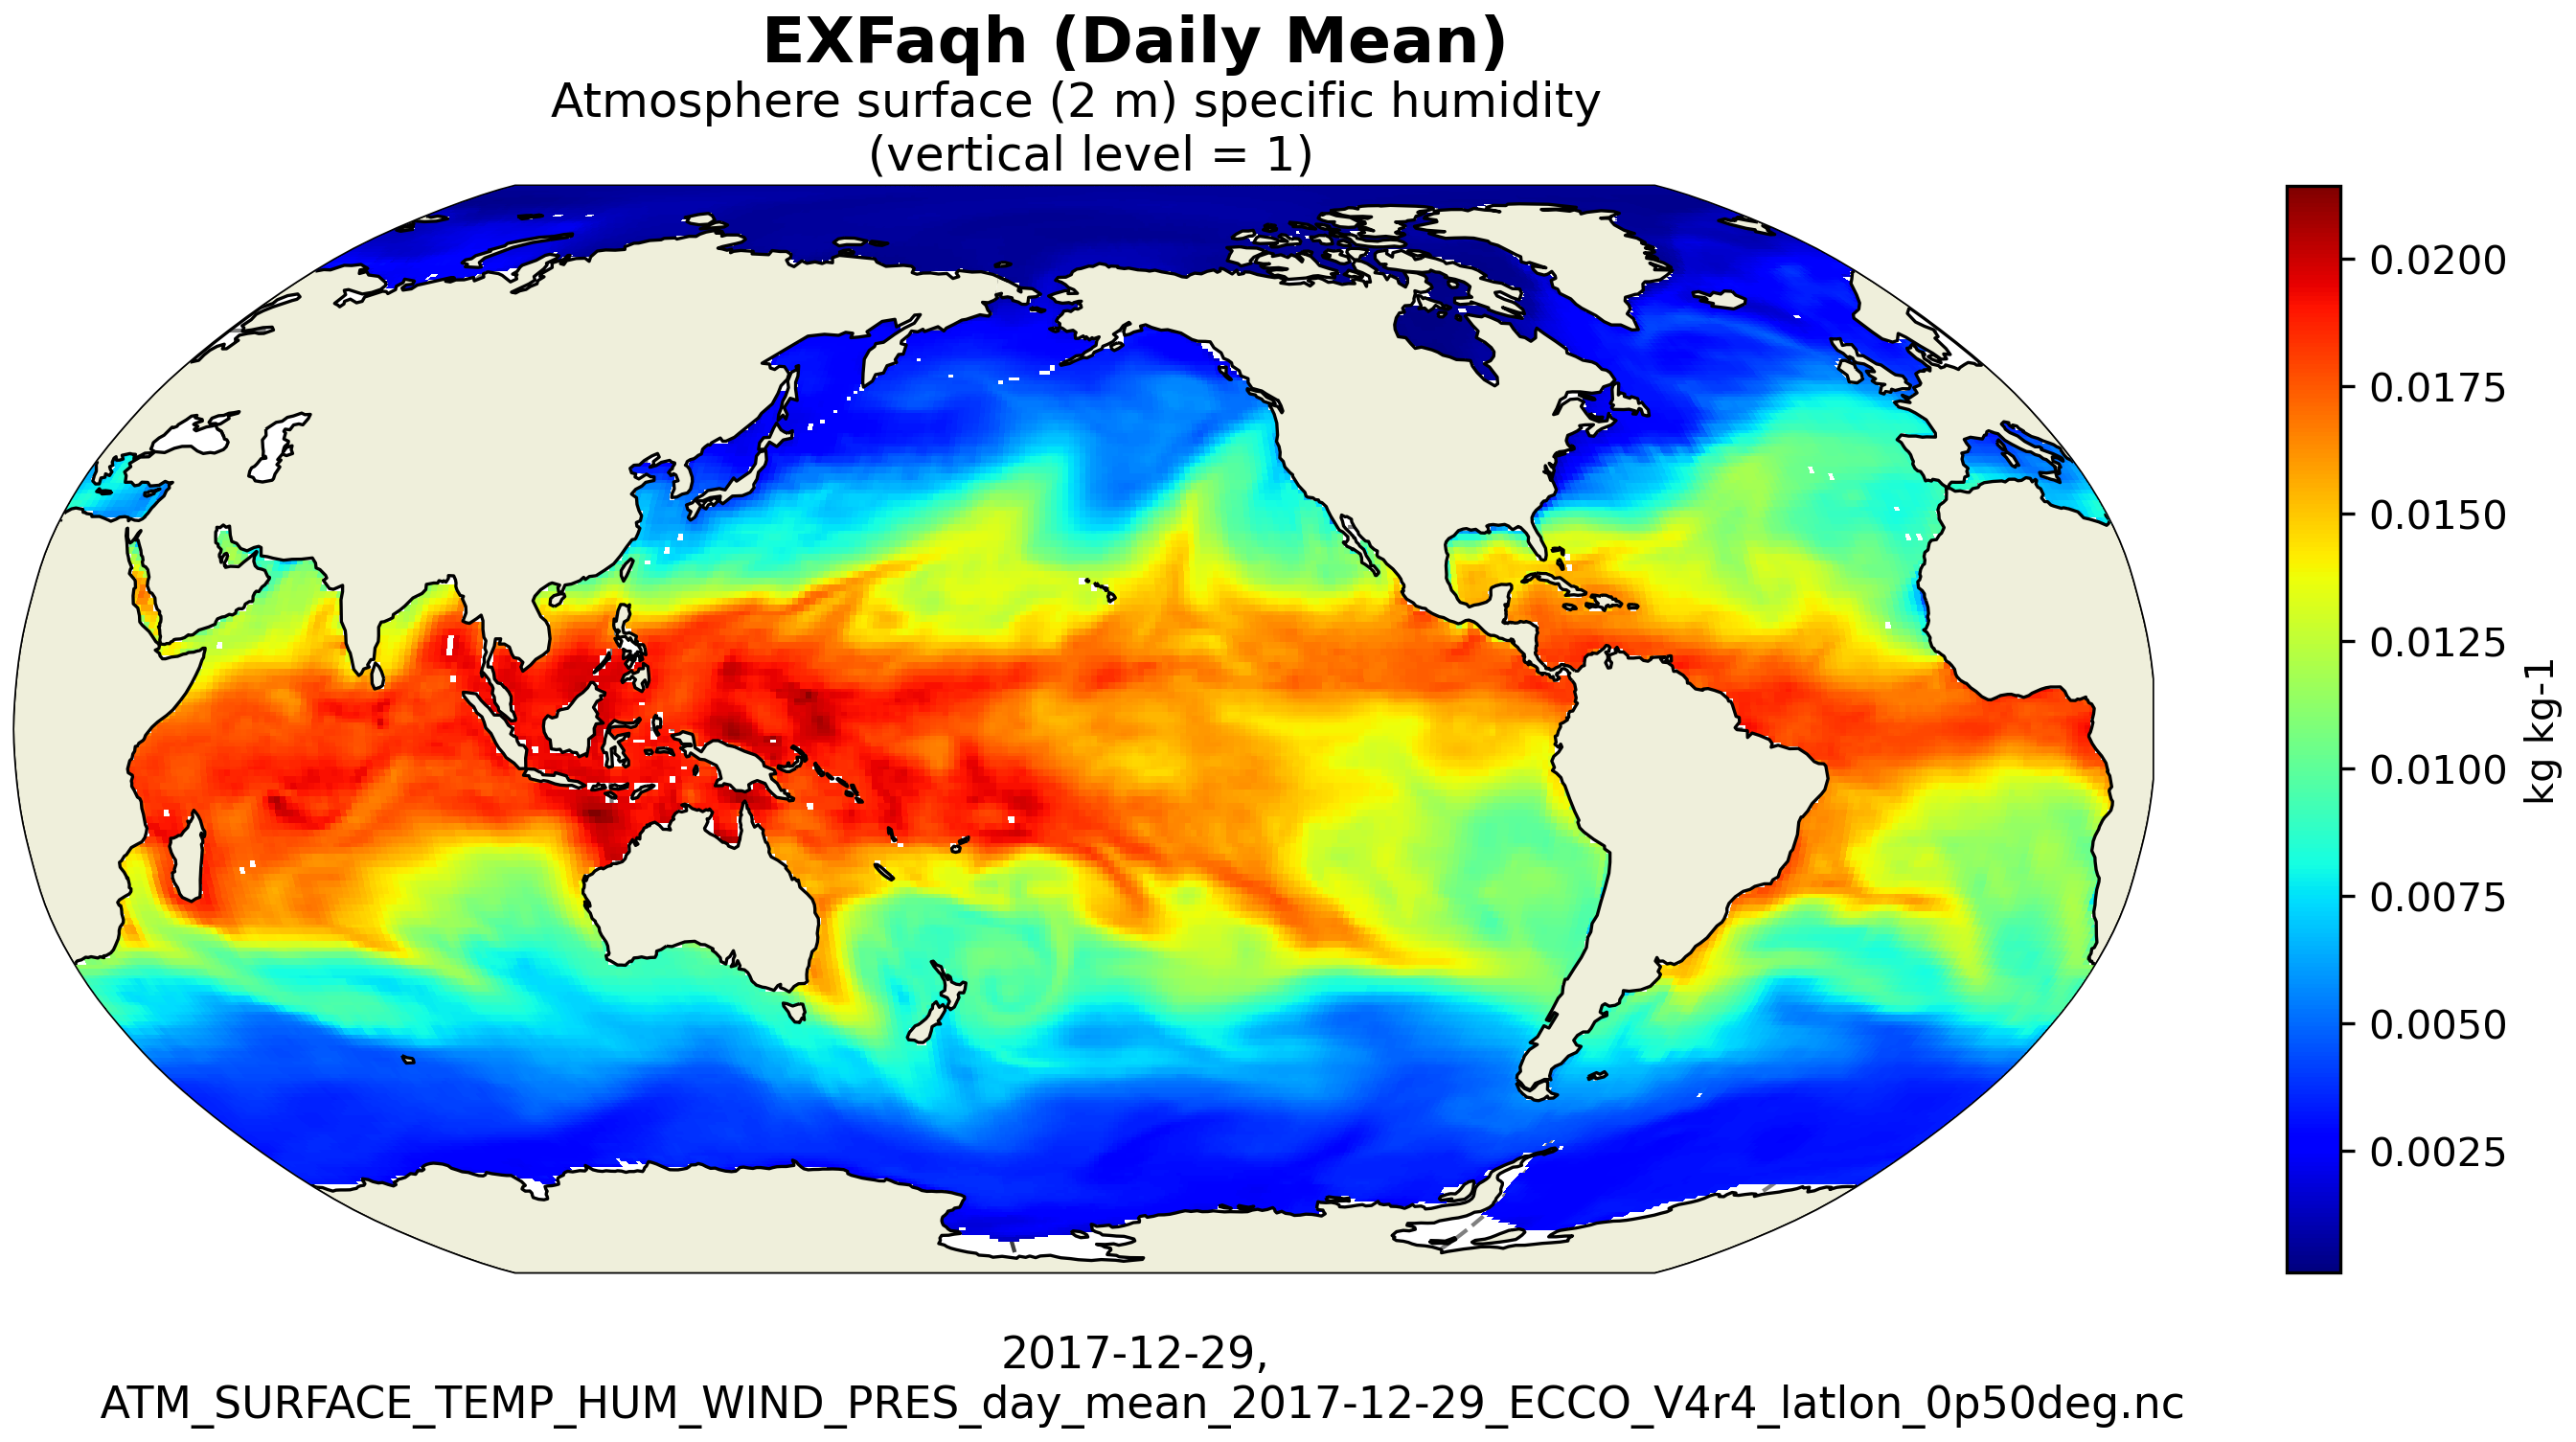
\includegraphics[scale=0.55]{../images/plots/v4r4/latlon_plots/Atmosphere_Surface_Temperature_Humidity_Wind_and_Pressure/EXFaqh.png}
\caption{Dataset: ATM\_SURFACE\_TEMP\_HUM\_WIND\_PRES, Variable: EXFaqh}
\label{tab:table-ATM_SURFACE_TEMP_HUM_WIND_PRES_EXFaqh-Plot}
\end{figure}
\newpage
\pagebreak
\subsubsection{Latlon Variable: EXFatemp}
\begin{longtable}{|m{0.06\textwidth}|m{0.3\textwidth}|m{0.45\textwidth}|m{0.12\textwidth}|}
\caption{Attributes description of the variable 'EXFatemp' from ATM\_SURFACE\_TEMP\_HUM\_WIND\_PRES's  dataset.}
\label{tab:table-ATM_SURFACE_TEMP_HUM_WIND_PRES_EXFatemp} \\ 
\hline \endhead \hline \endfoot
\rowcolor{lightgray} \textbf{Storage Type} & \textbf{Variable Name} & \textbf{Description} & \textbf{Unit} \\ \hline
float32 & EXFatemp & Atmosphere surface (2 m) air temperature  & degree\_K \\ \hline
\multicolumn{4}{|c|}{\cellcolor{lightgray}{\textbf{Description of the variable in Common Data language (CDL)}}} \\ \hline
\multicolumn{4}{|c|}{\fontfamily{lmtt}\selectfont{\makecell{\parbox{.95\textwidth}{\vspace*{0.25cm} \footnotesize{float32 EXFatemp(time, latitude, longitude)\\
\hspace*{0.5cm}EXFatemp: \_FillValue = 9.96921e+36\\
\hspace*{0.5cm}EXFatemp: coordinates = time\\
\hspace*{0.5cm}EXFatemp: coverage\_content\_type = modelResult\\
\hspace*{0.5cm}EXFatemp: long\_name = Atmosphere surface (2 m) air temperature \\
\hspace*{0.5cm}EXFatemp: standard\_name = air temperature\\
\hspace*{0.5cm}EXFatemp: units = degree K\\
\hspace*{0.5cm}EXFatemp: valid\_max = 312.8451232910156\\
\hspace*{0.5cm}EXFatemp: valid\_min = 195.37054443359375\\
}}}}} \\ \hline
\rowcolor{lightgray} \multicolumn{4}{|c|}{\textbf{Comments}} \\ \hline
\multicolumn{4}{|p{1\textwidth}|}{\footnotesize{{Surface (2 m) air temperature over open water. note: sum of era-interim surface air temperature and the control adjustment from ocean state estimation.}}} \\ \hline
\end{longtable}

\begin{figure}[H]
\centering
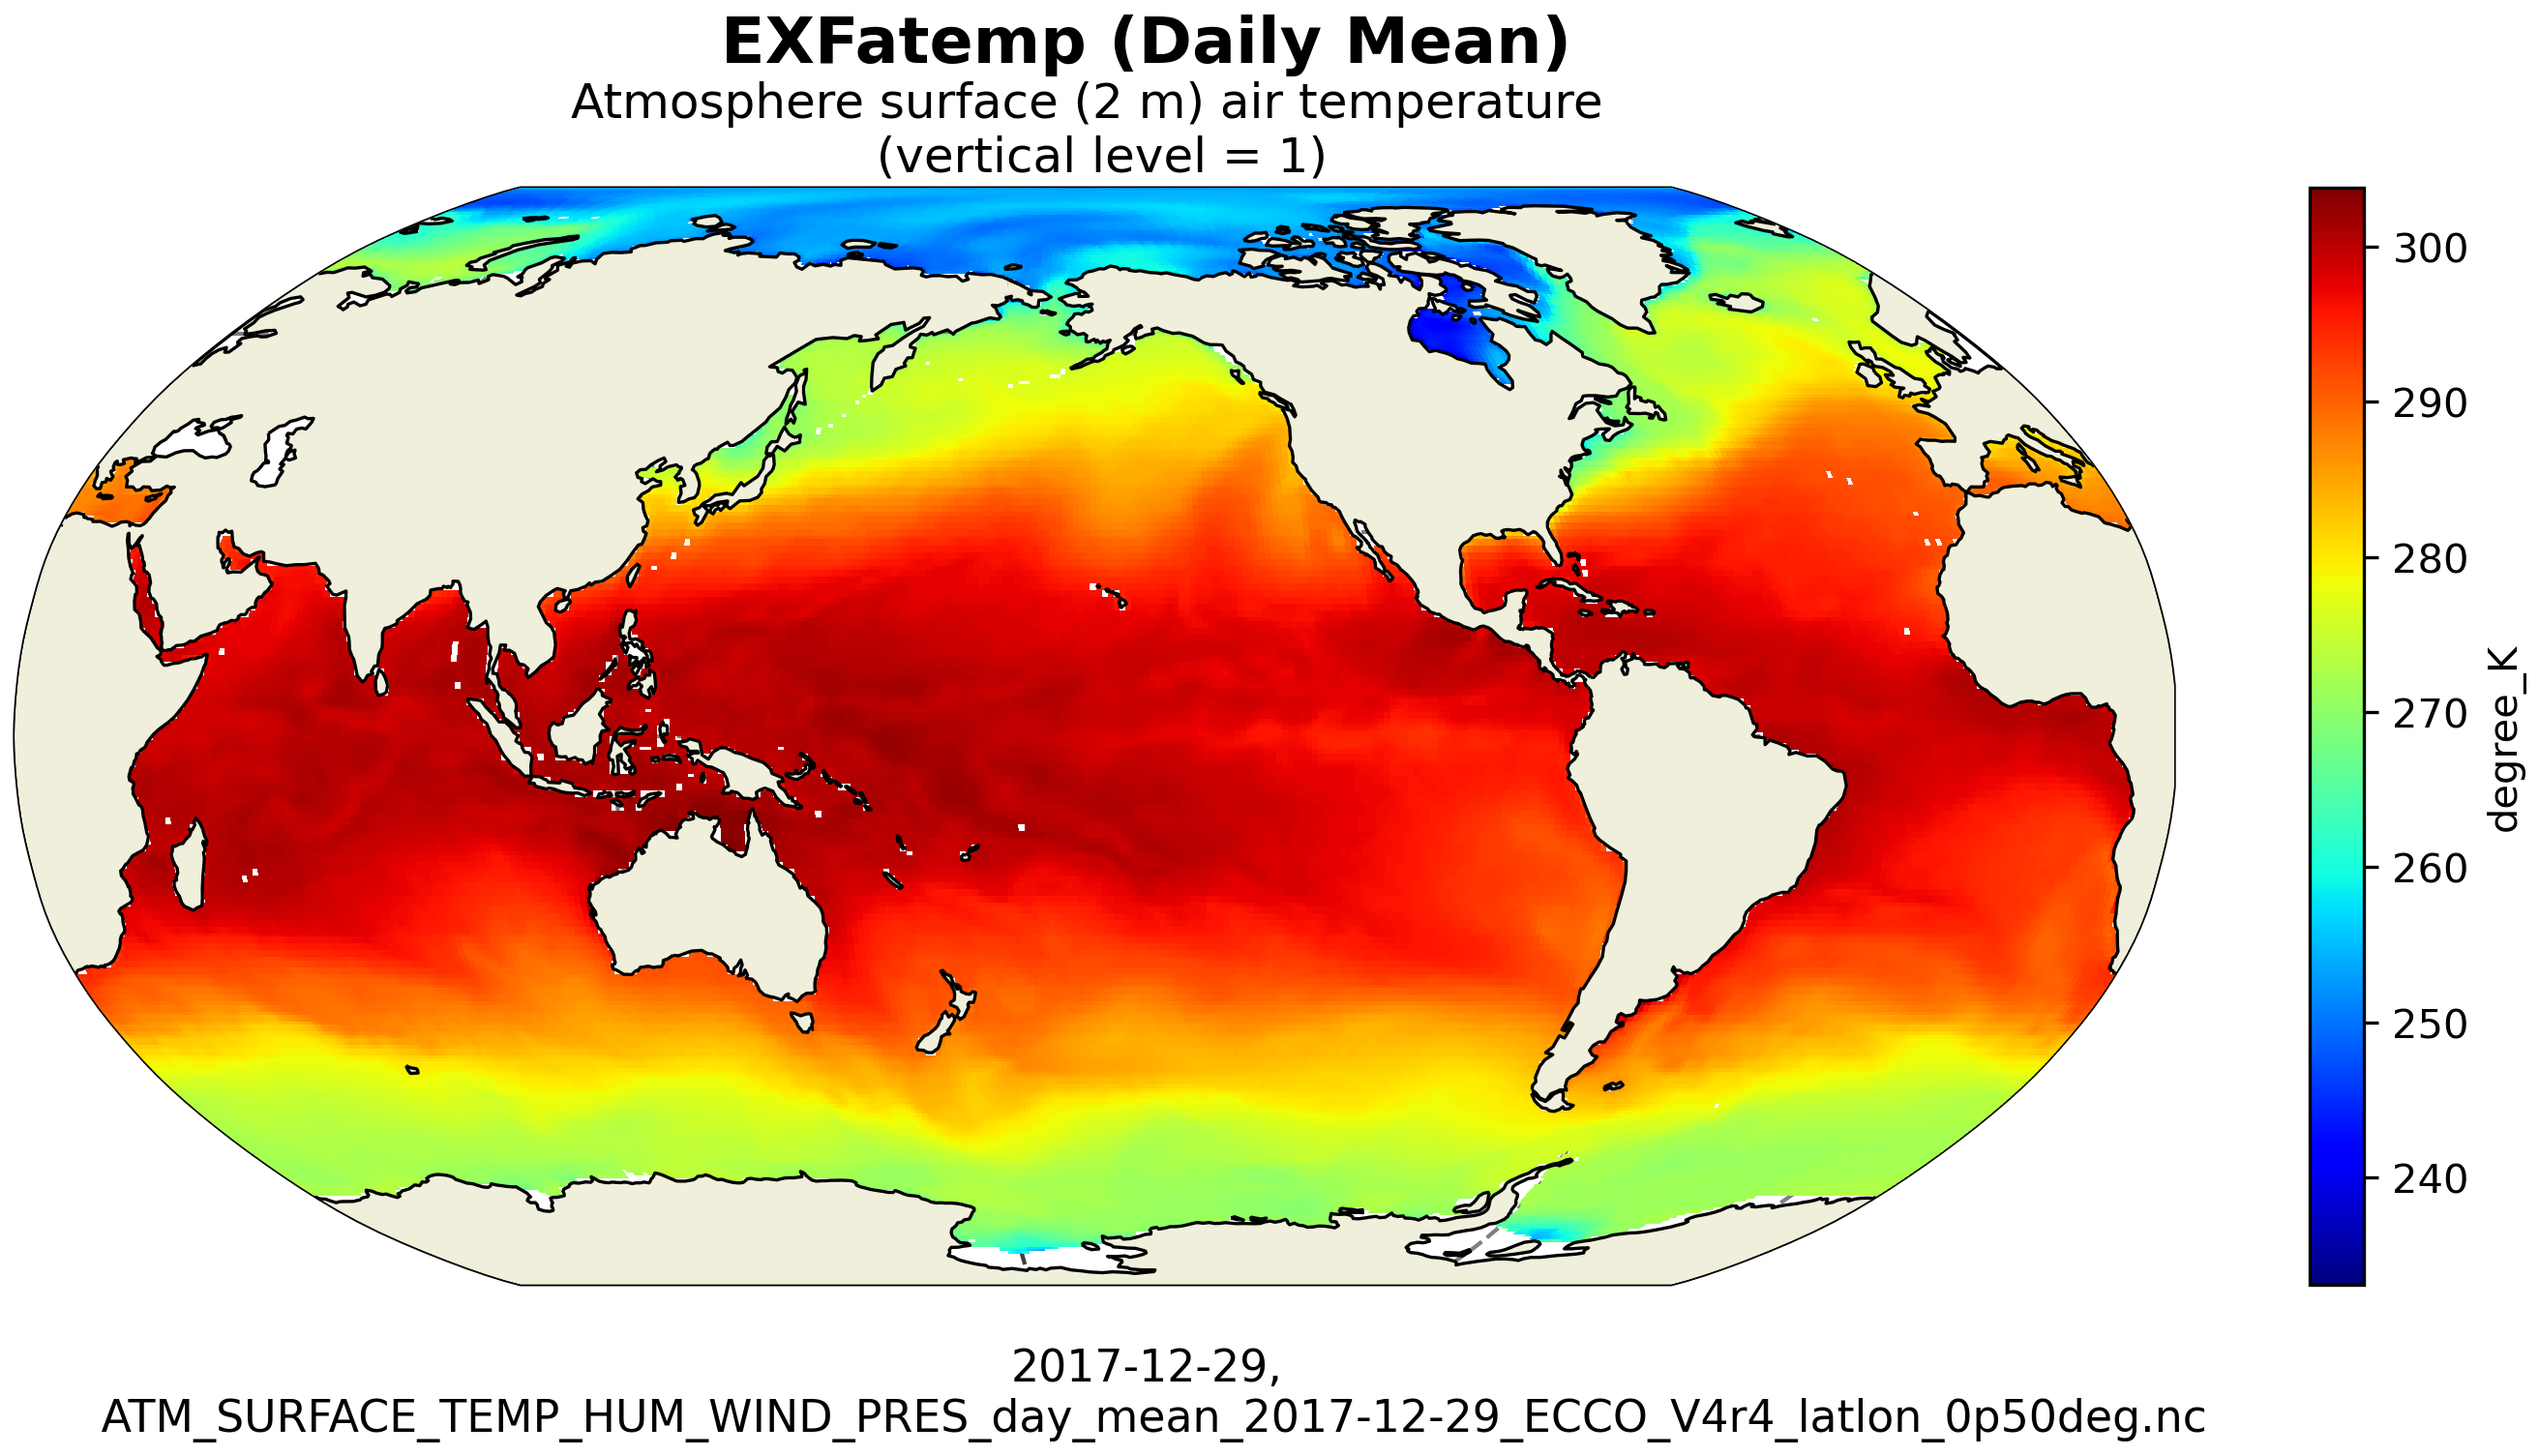
\includegraphics[scale=0.55]{../images/plots/v4r4/latlon_plots/Atmosphere_Surface_Temperature_Humidity_Wind_and_Pressure/EXFatemp.png}
\caption{Dataset: ATM\_SURFACE\_TEMP\_HUM\_WIND\_PRES, Variable: EXFatemp}
\label{tab:table-ATM_SURFACE_TEMP_HUM_WIND_PRES_EXFatemp-Plot}
\end{figure}
\newpage
\pagebreak
\subsubsection{Latlon Variable: EXFewind}
\begin{longtable}{|m{0.06\textwidth}|m{0.3\textwidth}|m{0.45\textwidth}|m{0.12\textwidth}|}
\caption{Attributes description of the variable 'EXFewind' from ATM\_SURFACE\_TEMP\_HUM\_WIND\_PRES's  dataset.}
\label{tab:table-ATM_SURFACE_TEMP_HUM_WIND_PRES_EXFewind} \\ 
\hline \endhead \hline \endfoot
\rowcolor{lightgray} \textbf{Storage Type} & \textbf{Variable Name} & \textbf{Description} & \textbf{Unit} \\ \hline
float32 & EXFewind & Zonal (east-west) wind speed & m s-1 \\ \hline
\multicolumn{4}{|c|}{\cellcolor{lightgray}{\textbf{Description of the variable in Common Data language (CDL)}}} \\ \hline
\multicolumn{4}{|c|}{\fontfamily{lmtt}\selectfont{\makecell{\parbox{.95\textwidth}{\vspace*{0.25cm} \footnotesize{float32 EXFewind(time, latitude, longitude)\\
\hspace*{0.5cm}EXFewind: \_FillValue = 9.96921e+36\\
\hspace*{0.5cm}EXFewind: coordinates = time\\
\hspace*{0.5cm}EXFewind: coverage\_content\_type = modelResult\\
\hspace*{0.5cm}EXFewind: long\_name = Zonal (east-west) wind speed\\
\hspace*{0.5cm}EXFewind: standard\_name = eastward wind\\
\hspace*{0.5cm}EXFewind: units = m s-1\\
\hspace*{0.5cm}EXFewind: valid\_max = 39.48556900024414\\
\hspace*{0.5cm}EXFewind: valid\_min = -33.524742126464844\\
}}}}} \\ \hline
\rowcolor{lightgray} \multicolumn{4}{|c|}{\textbf{Comments}} \\ \hline
\multicolumn{4}{|p{1\textwidth}|}{\footnotesize{{Zonal (east-west) component of ocean surface wind. note: exfewind is calculated by interpolating the model's x and y components of wind velocity (exfuwind and exfvwind) to tracer cell centers and then finding the zonal component of the interpolated vectors. ecco v4r4 is forced with wind stress (see exftaux, exftauy), not vector winds + bulk formulae. exfewind is calculated by converting wind stress to vector wind using bulk formulae.}}} \\ \hline
\end{longtable}

\begin{figure}[H]
\centering
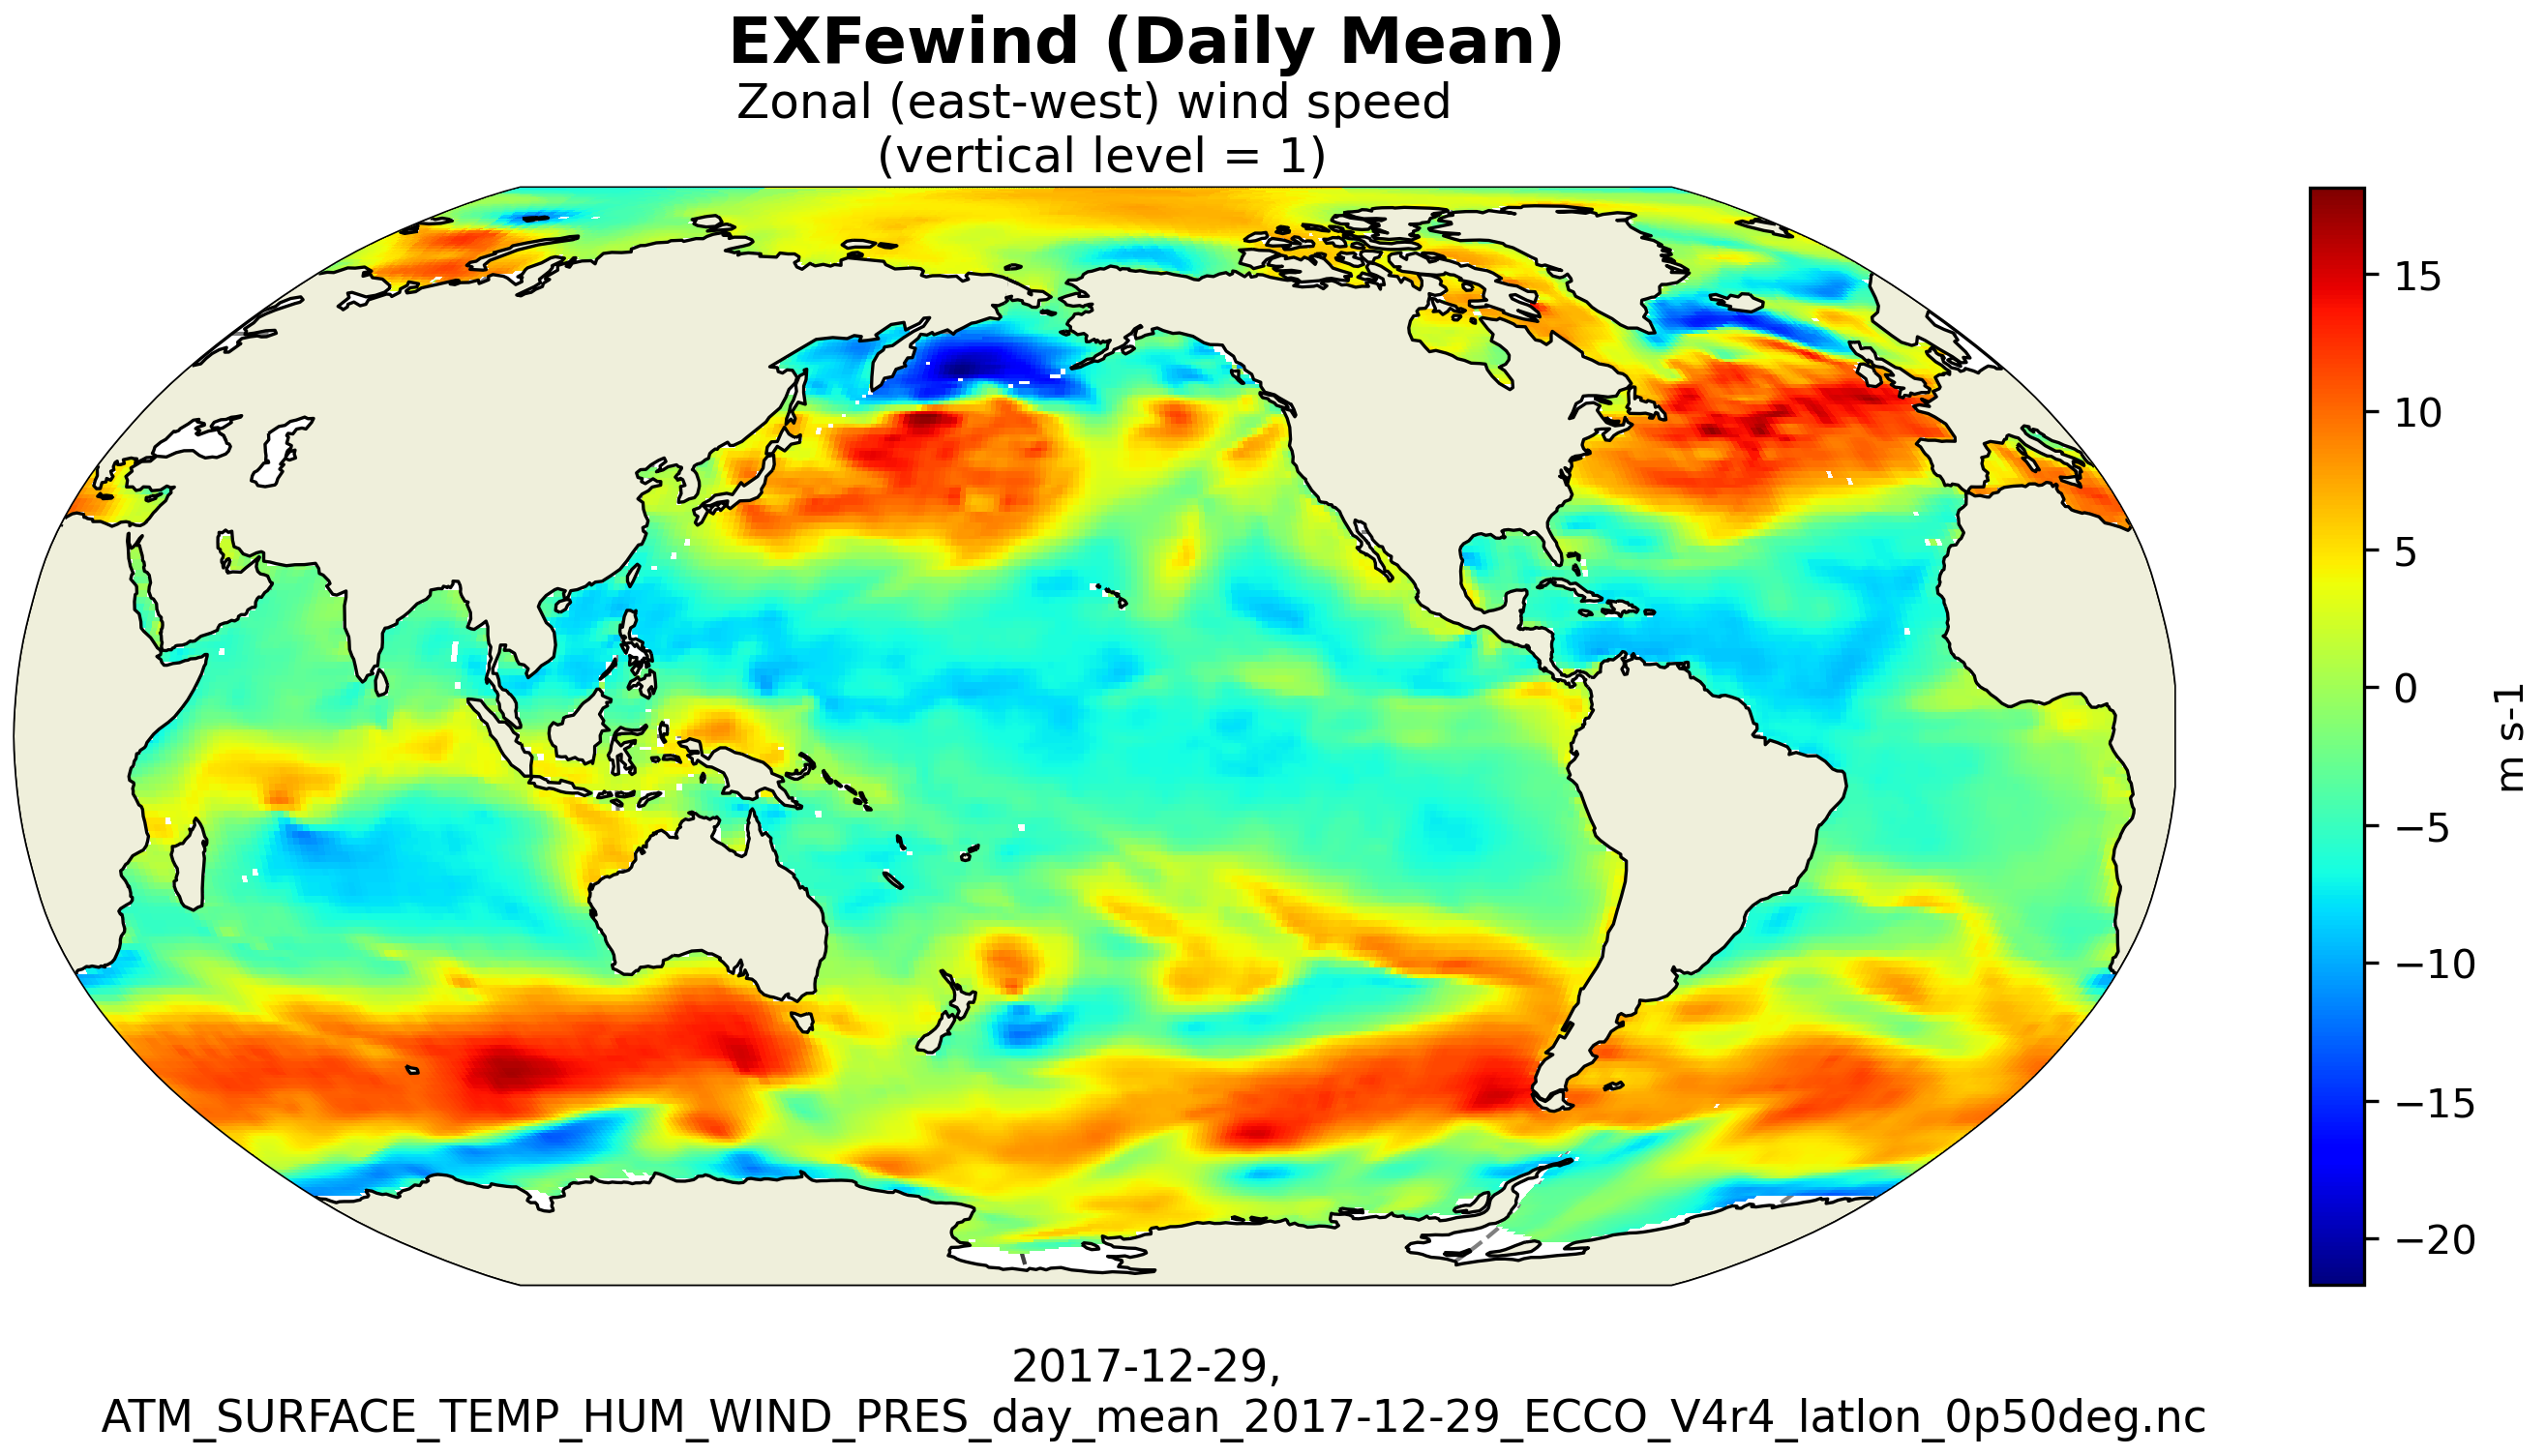
\includegraphics[scale=0.55]{../images/plots/v4r4/latlon_plots/Atmosphere_Surface_Temperature_Humidity_Wind_and_Pressure/EXFewind.png}
\caption{Dataset: ATM\_SURFACE\_TEMP\_HUM\_WIND\_PRES, Variable: EXFewind}
\label{tab:table-ATM_SURFACE_TEMP_HUM_WIND_PRES_EXFewind-Plot}
\end{figure}
\newpage
\pagebreak
\subsubsection{Latlon Variable: EXFnwind}
\begin{longtable}{|m{0.06\textwidth}|m{0.3\textwidth}|m{0.45\textwidth}|m{0.12\textwidth}|}
\caption{Attributes description of the variable 'EXFnwind' from ATM\_SURFACE\_TEMP\_HUM\_WIND\_PRES's  dataset.}
\label{tab:table-ATM_SURFACE_TEMP_HUM_WIND_PRES_EXFnwind} \\ 
\hline \endhead \hline \endfoot
\rowcolor{lightgray} \textbf{Storage Type} & \textbf{Variable Name} & \textbf{Description} & \textbf{Unit} \\ \hline
float32 & EXFnwind & Meridional (north-south) wind speed & m s-1 \\ \hline
\multicolumn{4}{|c|}{\cellcolor{lightgray}{\textbf{Description of the variable in Common Data language (CDL)}}} \\ \hline
\multicolumn{4}{|c|}{\fontfamily{lmtt}\selectfont{\makecell{\parbox{.95\textwidth}{\vspace*{0.25cm} \footnotesize{float32 EXFnwind(time, latitude, longitude)\\
\hspace*{0.5cm}EXFnwind: \_FillValue = 9.96921e+36\\
\hspace*{0.5cm}EXFnwind: coordinates = time\\
\hspace*{0.5cm}EXFnwind: coverage\_content\_type = modelResult\\
\hspace*{0.5cm}EXFnwind: long\_name = Meridional (north-south) wind speed\\
\hspace*{0.5cm}EXFnwind: standard\_name = northward wind\\
\hspace*{0.5cm}EXFnwind: units = m s-1\\
\hspace*{0.5cm}EXFnwind: valid\_max = 33.95014190673828\\
\hspace*{0.5cm}EXFnwind: valid\_min = -30.042686462402344\\
}}}}} \\ \hline
\rowcolor{lightgray} \multicolumn{4}{|c|}{\textbf{Comments}} \\ \hline
\multicolumn{4}{|p{1\textwidth}|}{\footnotesize{{Meridional (north-south) component of ocean surface wind. note: exfnwind is calculated by interpolating the model's x and y components of wind velocity (exfuwind and exfvwind) to tracer cell centers and then finding the meridional component of the interpolated vectors. ecco v4r4 is forced with wind stress (see exftaux, exftauy), not vector winds + bulk formulae.  exfnwind is calculated by converting wind stress to vector wind using bulk formulae.}}} \\ \hline
\end{longtable}

\begin{figure}[H]
\centering
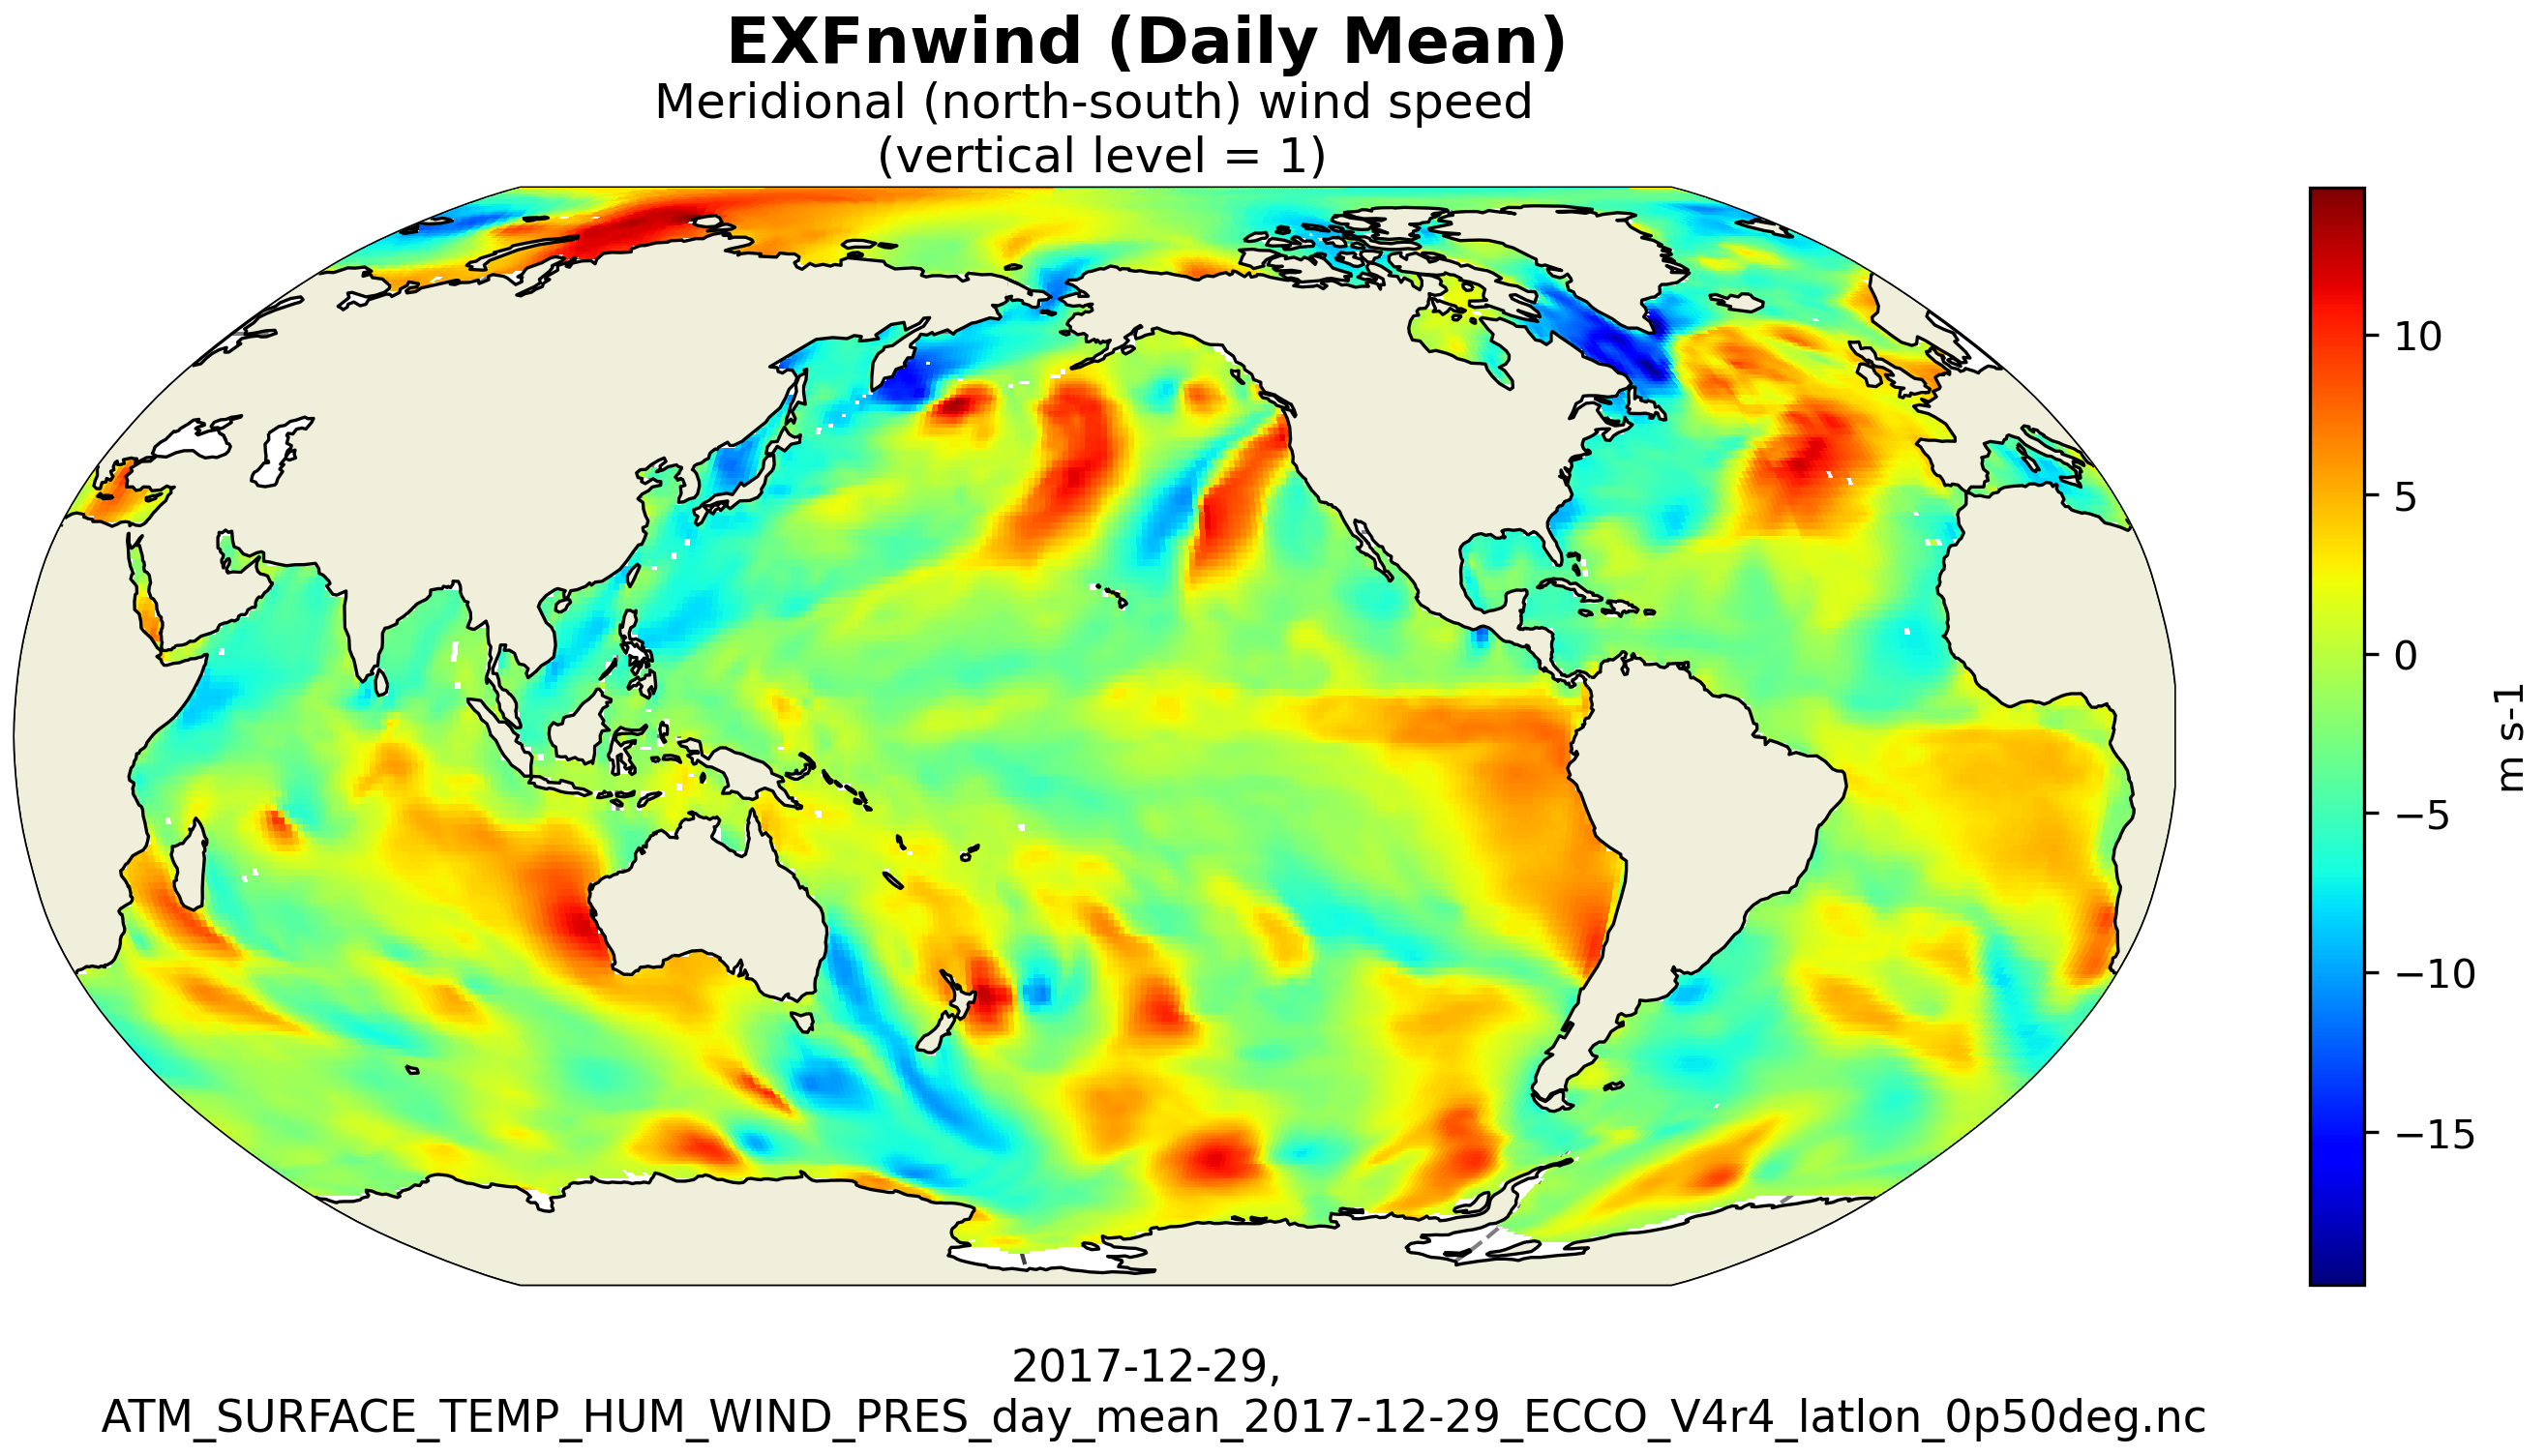
\includegraphics[scale=0.55]{../images/plots/v4r4/latlon_plots/Atmosphere_Surface_Temperature_Humidity_Wind_and_Pressure/EXFnwind.png}
\caption{Dataset: ATM\_SURFACE\_TEMP\_HUM\_WIND\_PRES, Variable: EXFnwind}
\label{tab:table-ATM_SURFACE_TEMP_HUM_WIND_PRES_EXFnwind-Plot}
\end{figure}
\newpage
\pagebreak
\subsubsection{Latlon Variable: EXFpress}
\begin{longtable}{|m{0.06\textwidth}|m{0.3\textwidth}|m{0.45\textwidth}|m{0.12\textwidth}|}
\caption{Attributes description of the variable 'EXFpress' from ATM\_SURFACE\_TEMP\_HUM\_WIND\_PRES's  dataset.}
\label{tab:table-ATM_SURFACE_TEMP_HUM_WIND_PRES_EXFpress} \\ 
\hline \endhead \hline \endfoot
\rowcolor{lightgray} \textbf{Storage Type} & \textbf{Variable Name} & \textbf{Description} & \textbf{Unit} \\ \hline
float32 & EXFpress & Atmosphere surface pressure & N m-2 \\ \hline
\multicolumn{4}{|c|}{\cellcolor{lightgray}{\textbf{Description of the variable in Common Data language (CDL)}}} \\ \hline
\multicolumn{4}{|c|}{\fontfamily{lmtt}\selectfont{\makecell{\parbox{.95\textwidth}{\vspace*{0.25cm} \footnotesize{float32 EXFpress(time, latitude, longitude)\\
\hspace*{0.5cm}EXFpress: \_FillValue = 9.96921e+36\\
\hspace*{0.5cm}EXFpress: coordinates = time\\
\hspace*{0.5cm}EXFpress: coverage\_content\_type = modelResult\\
\hspace*{0.5cm}EXFpress: long\_name = Atmosphere surface pressure\\
\hspace*{0.5cm}EXFpress: standard\_name = surface air pressure\\
\hspace*{0.5cm}EXFpress: units = N m-2\\
\hspace*{0.5cm}EXFpress: valid\_max = 106314.7734375\\
\hspace*{0.5cm}EXFpress: valid\_min = 92090.3125\\
}}}}} \\ \hline
\rowcolor{lightgray} \multicolumn{4}{|c|}{\textbf{Comments}} \\ \hline
\multicolumn{4}{|p{1\textwidth}|}{\footnotesize{{Atmospheric pressure field at sea level. note: era-interim atmospheric pressure, with air tides removed using a variety of methods. not adjusted by the ocean state estimation.}}} \\ \hline
\end{longtable}

\begin{figure}[H]
\centering
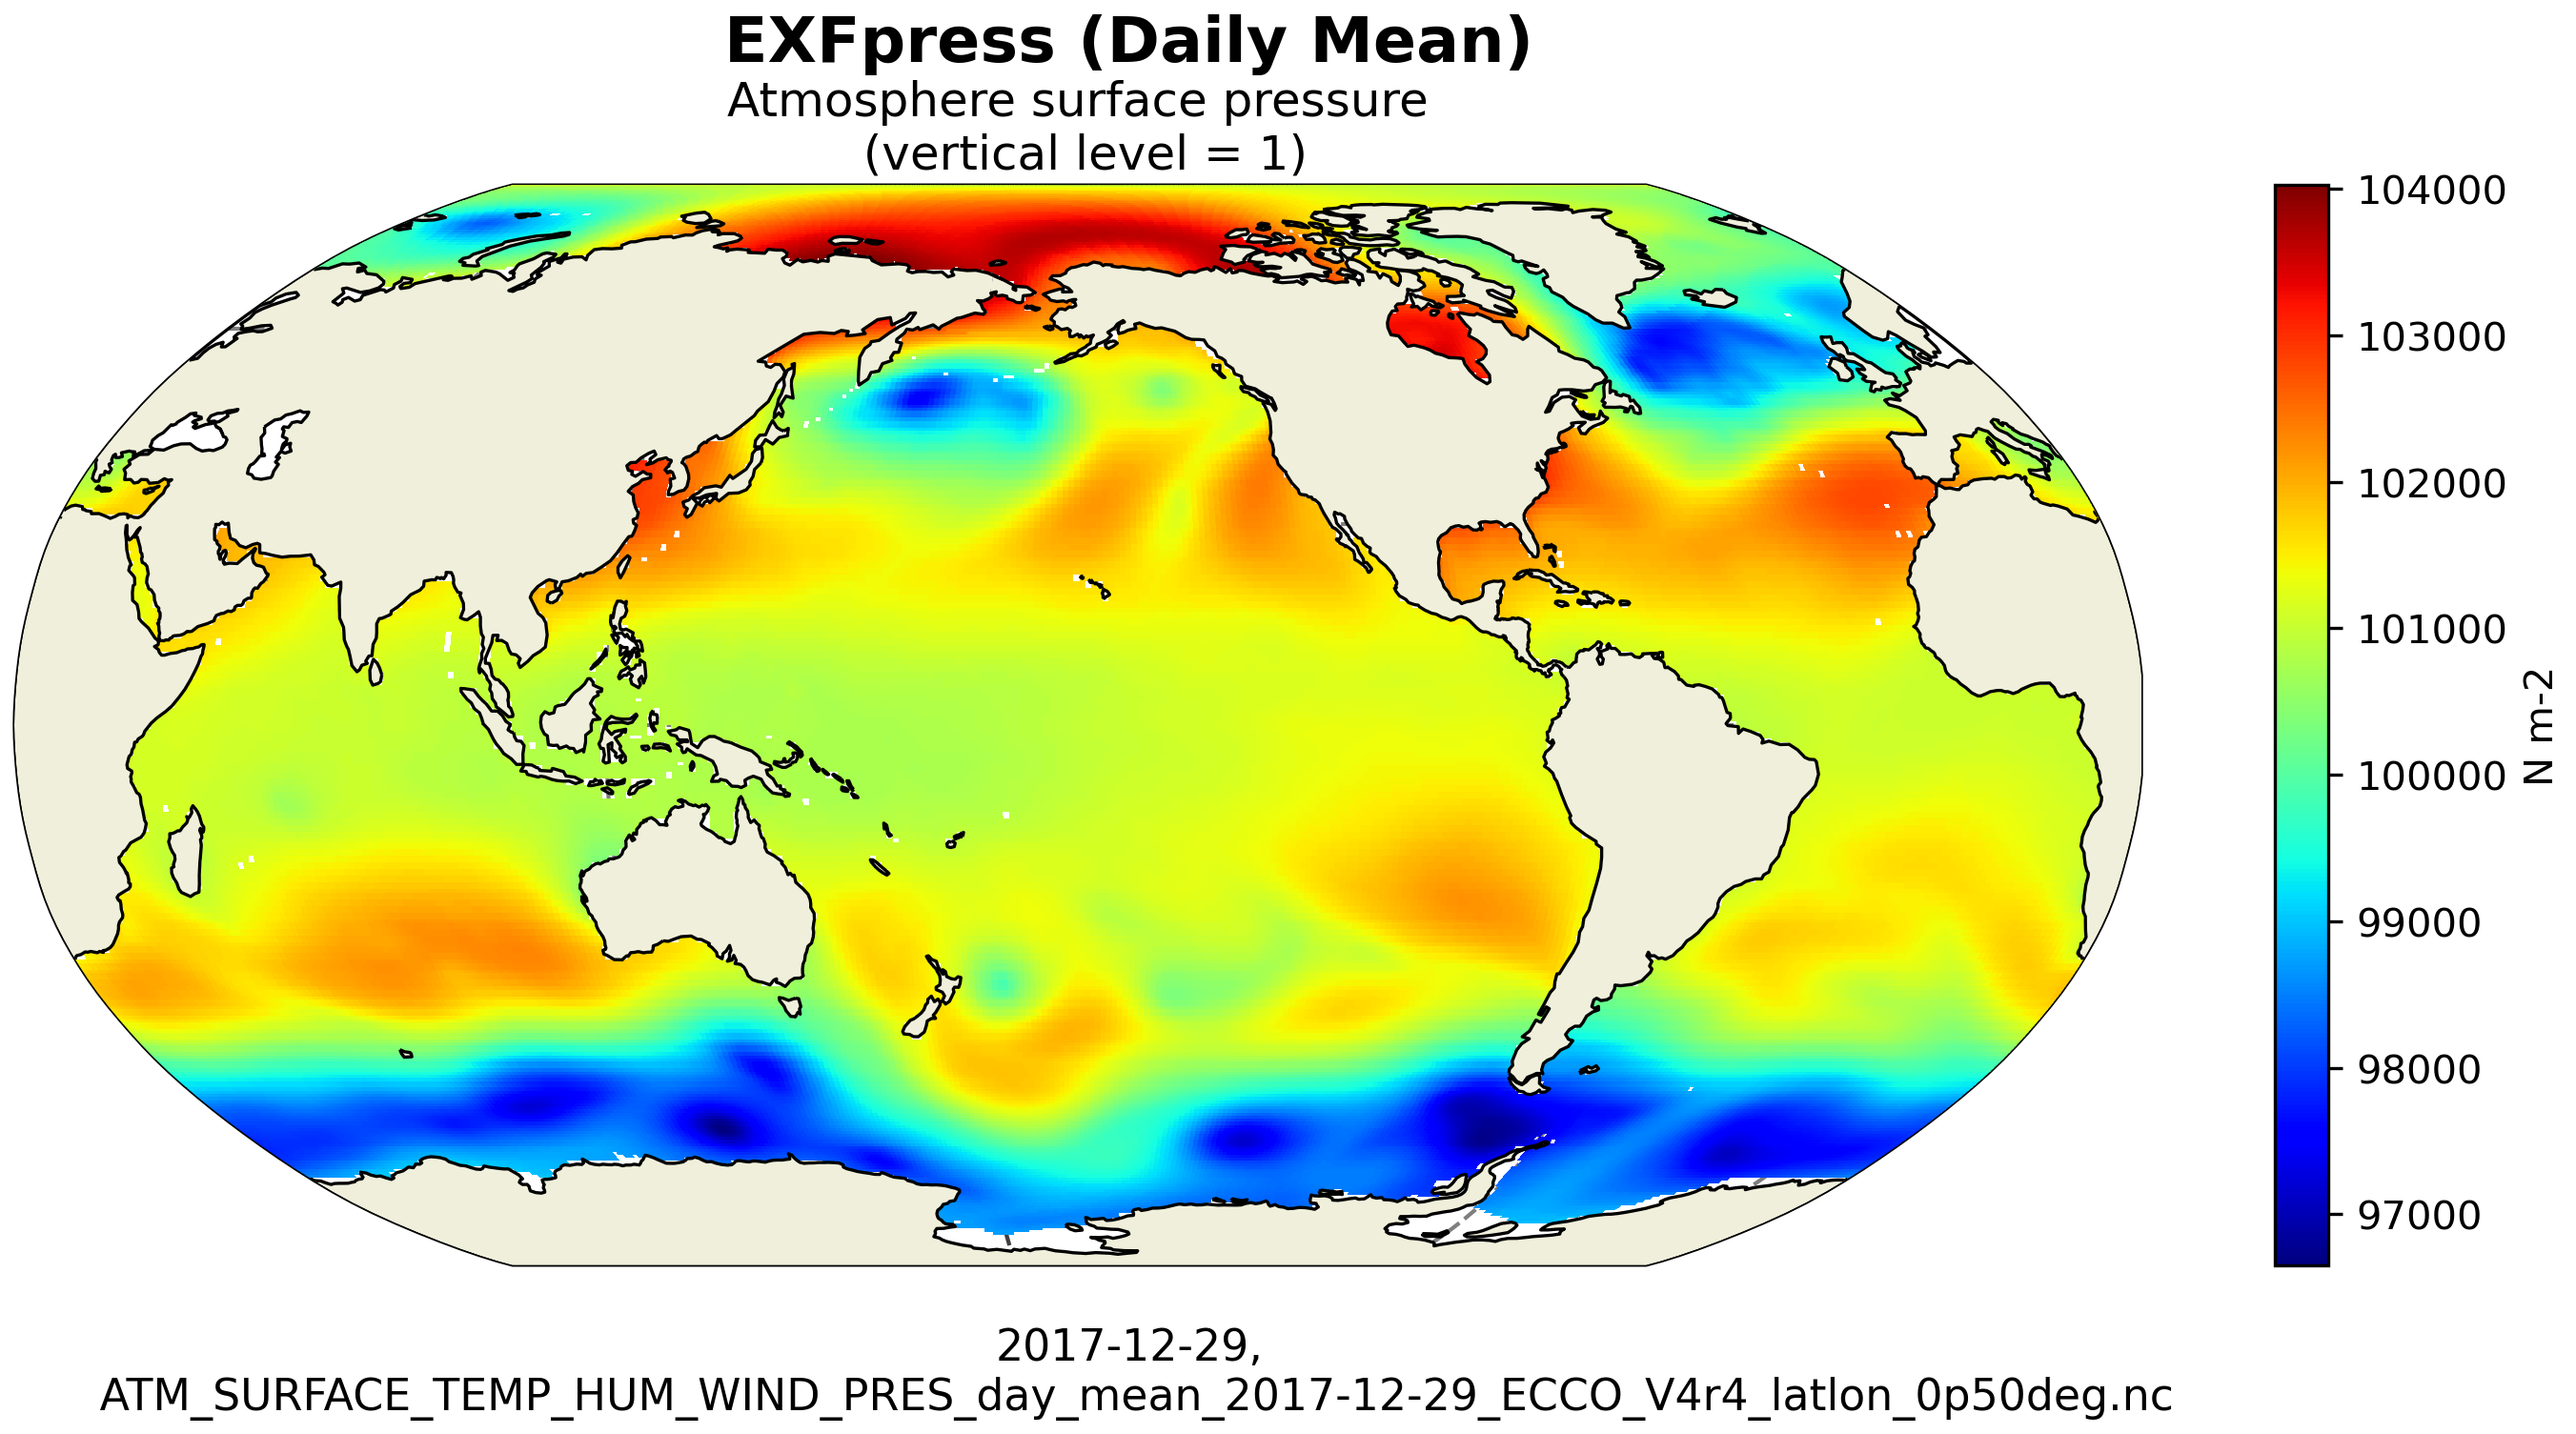
\includegraphics[scale=0.55]{../images/plots/v4r4/latlon_plots/Atmosphere_Surface_Temperature_Humidity_Wind_and_Pressure/EXFpress.png}
\caption{Dataset: ATM\_SURFACE\_TEMP\_HUM\_WIND\_PRES, Variable: EXFpress}
\label{tab:table-ATM_SURFACE_TEMP_HUM_WIND_PRES_EXFpress-Plot}
\end{figure}
\newpage
\pagebreak
\subsubsection{Latlon Variable: EXFwspee}
\begin{longtable}{|m{0.06\textwidth}|m{0.3\textwidth}|m{0.45\textwidth}|m{0.12\textwidth}|}
\caption{Attributes description of the variable 'EXFwspee' from ATM\_SURFACE\_TEMP\_HUM\_WIND\_PRES's  dataset.}
\label{tab:table-ATM_SURFACE_TEMP_HUM_WIND_PRES_EXFwspee} \\ 
\hline \endhead \hline \endfoot
\rowcolor{lightgray} \textbf{Storage Type} & \textbf{Variable Name} & \textbf{Description} & \textbf{Unit} \\ \hline
float32 & EXFwspee & Wind speed & m s-1 \\ \hline
\multicolumn{4}{|c|}{\cellcolor{lightgray}{\textbf{Description of the variable in Common Data language (CDL)}}} \\ \hline
\multicolumn{4}{|c|}{\fontfamily{lmtt}\selectfont{\makecell{\parbox{.95\textwidth}{\vspace*{0.25cm} \footnotesize{float32 EXFwspee(time, latitude, longitude)\\
\hspace*{0.5cm}EXFwspee: \_FillValue = 9.96921e+36\\
\hspace*{0.5cm}EXFwspee: coordinates = time\\
\hspace*{0.5cm}EXFwspee: coverage\_content\_type = modelResult\\
\hspace*{0.5cm}EXFwspee: long\_name = Wind speed\\
\hspace*{0.5cm}EXFwspee: standard\_name = wind speed\\
\hspace*{0.5cm}EXFwspee: units = m s-1\\
\hspace*{0.5cm}EXFwspee: valid\_max = 45.87086486816406\\
\hspace*{0.5cm}EXFwspee: valid\_min = 0.27271032333374023\\
}}}}} \\ \hline
\rowcolor{lightgray} \multicolumn{4}{|c|}{\textbf{Comments}} \\ \hline
\multicolumn{4}{|p{1\textwidth}|}{\footnotesize{{10-m wind speed magnitude (>= 0 ) over open water. only used for the calculation of air-sea fluxes using bulk formulae. note: not adjusted by the ocean state estimation and not necesarily consistent with exfuwind and exfvwind because exfuwind and exfvwind are calculated from exftaux and exftauy using bulk formulae. exfwspee != sqrt(exfuwind**2 + exfvwind**2.}}} \\ \hline
\end{longtable}

\begin{figure}[H]
\centering
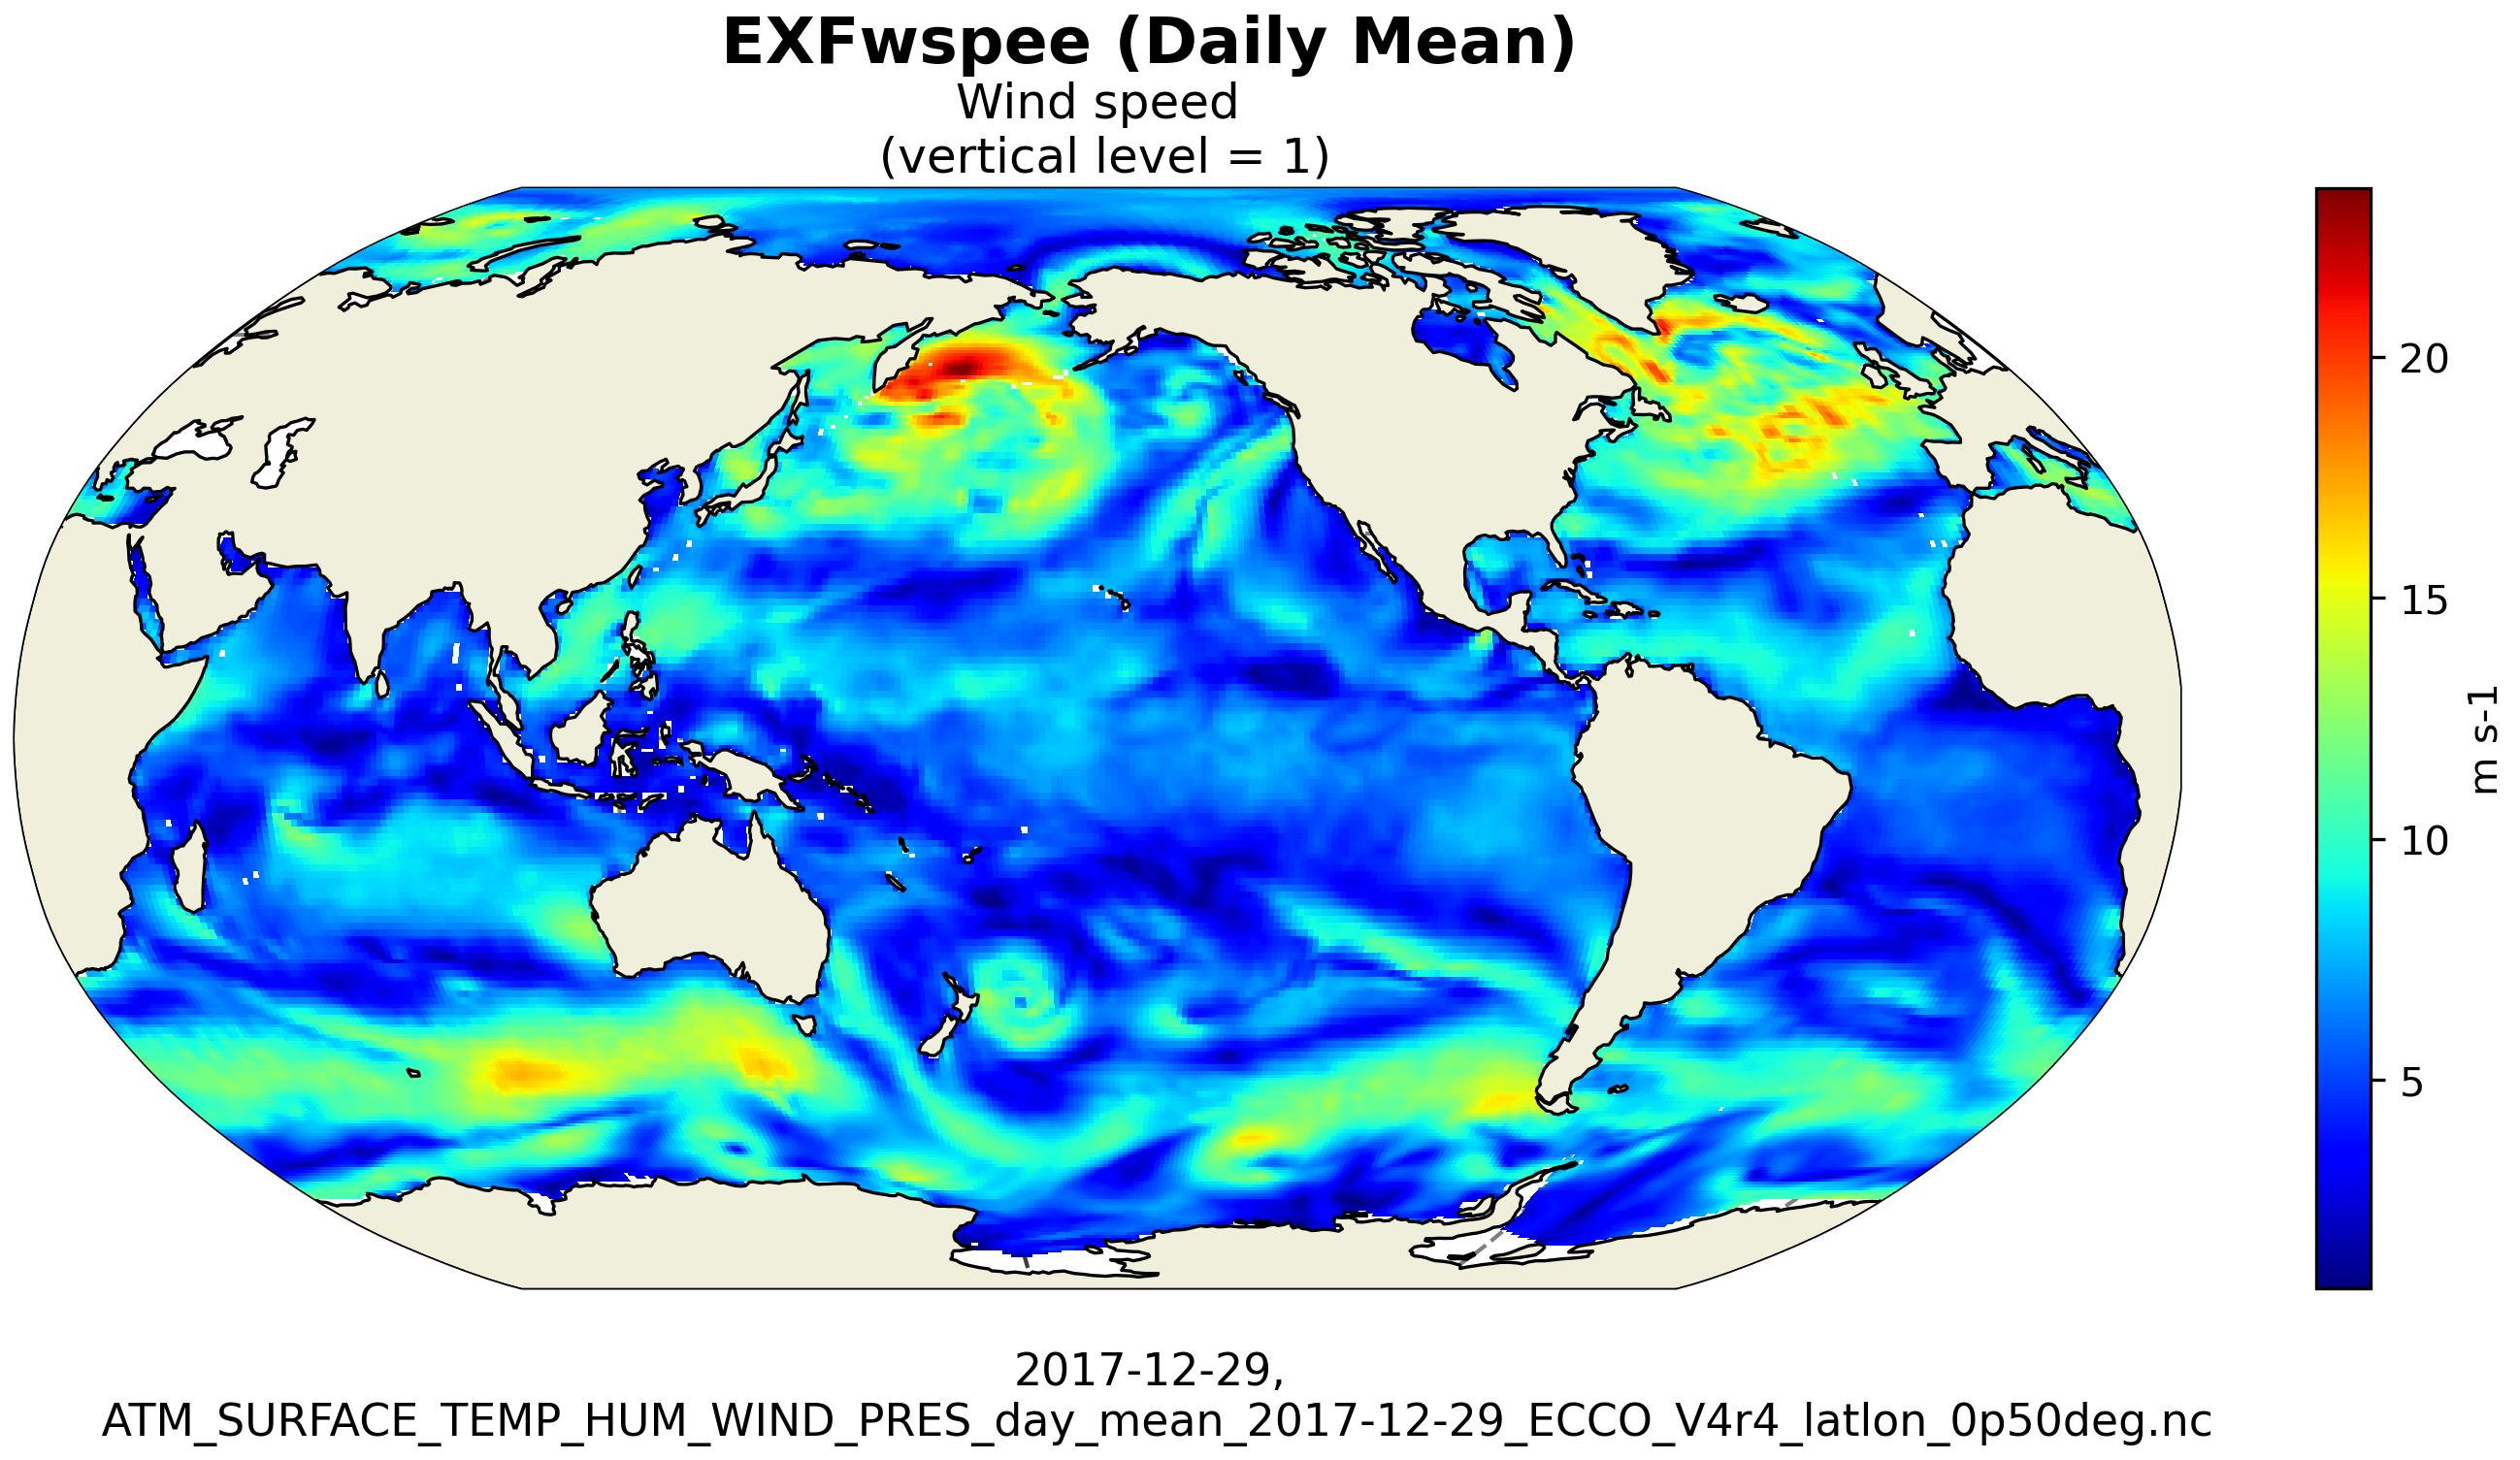
\includegraphics[scale=0.55]{../images/plots/v4r4/latlon_plots/Atmosphere_Surface_Temperature_Humidity_Wind_and_Pressure/EXFwspee.png}
\caption{Dataset: ATM\_SURFACE\_TEMP\_HUM\_WIND\_PRES, Variable: EXFwspee}
\label{tab:table-ATM_SURFACE_TEMP_HUM_WIND_PRES_EXFwspee-Plot}
\end{figure}
\newpage
\subsection{Latlon dataset of OCEAN\_AND\_ICE\_SURFACE\_FW\_FLUX}
\newp
\subsubsection{Overview}
This dataset provides 2D fields of ocean and sea-ice surface freshwater fluxes interpolated to a regular 0.5-degree grid from the ECCO Version 4 Release 4 (V4r4) ocean and sea-ice state estimate. The dataset is provided on daily-average and monthly-average time resolution. 
\begin{longtable}{|m{0.15\textwidth}|m{0.64\textwidth}|m{0.12\textwidth}|}
\caption{Coordinates and Variables in the dataset OCEAN\_AND\_ICE\_SURFACE\_FW\_FLUX}
\label{tab:table-OCEAN_AND_ICE_SURFACE_FW_FLUX-fields} \\ 
\hline \endhead \hline \endfoot
\rowcolor{lightgray} \multicolumn{1}{|c|}{\textbf{Coordinates}} & \multicolumn{1}{|c|}{\textbf{Description of data coordinates}} &  \multicolumn{1}{|c|}{\textbf{Unit}}\\ \hline
time &Center time of averaging period &--none--  \\ \hline
latitude &Latitude at grid cell center &degrees\_north  \\ \hline
longitude &Longitude at grid cell center &degrees\_east  \\ \hline
time\_bnds &Time bounds of averaging period &--none--  \\ \hline
latitude\_bnds &Latitude bounds grid cells &--none--  \\ \hline
longitude\_bnds &Longitude bounds grid cells &--none--  \\ \hline
\rowcolor{lightgray} \multicolumn{1}{|c|}{\textbf{Variables}} & \multicolumn{1}{|c|}{\textbf{Description of data variables}} &  \multicolumn{1}{|c|}{\textbf{Unit}}\\ \hline
EXFpreci &Precipitation rate &m s-1  \\ \hline
EXFevap &Open ocean evaporation rate &m s-1  \\ \hline
EXFroff &River runoff &m s-1  \\ \hline
SIsnPrcp &Snow precipitation on sea-ice &kg m-2 s-1  \\ \hline
EXFempmr &Open ocean net surface freshwater flux from precipitation, evaporation, and runoff &m s-1  \\ \hline
oceFWflx &Net freshwater flux into the ocean &kg m-2 s-1  \\ \hline
SIatmFW &Net freshwater flux into the open ocean, sea-ice, and snow &kg m-2 s-1  \\ \hline
SFLUX &Rate of change of total ocean salinity per m2 accounting for mass fluxes. &g m-2 s-1  \\ \hline
SIacSubl &Freshwater flux to the atmosphere due to sublimation-deposition of snow or ice &kg m-2 s-1  \\ \hline
SIrsSubl &Residual sublimation freshwater flux &kg m-2 s-1  \\ \hline
SIfwThru &Precipitation through sea-ice &kg m-2 s-1  \\ \hline
\end{longtable}

\newp
\pagebreak
\subsubsection{Latlon Variable: EXFempmr}
\begin{longtable}{|m{0.06\textwidth}|m{0.3\textwidth}|m{0.45\textwidth}|m{0.12\textwidth}|}
\caption{Attributes description of the variable 'EXFempmr' from OCEAN\_AND\_ICE\_SURFACE\_FW\_FLUX's  dataset.}
\label{tab:table-OCEAN_AND_ICE_SURFACE_FW_FLUX_EXFempmr} \\ 
\hline \endhead \hline \endfoot
\rowcolor{lightgray} \textbf{Storage Type} & \textbf{Variable Name} & \textbf{Description} & \textbf{Unit} \\ \hline
float32 & EXFempmr & Open ocean net surface freshwater flux from precipitation, evaporation, and runoff & m s-1 \\ \hline
\multicolumn{4}{|c|}{\cellcolor{lightgray}{\textbf{Description of the variable in Common Data language (CDL)}}} \\ \hline
\multicolumn{4}{|c|}{\fontfamily{lmtt}\selectfont{\makecell{\parbox{.95\textwidth}{\vspace*{0.25cm} \footnotesize{float32 EXFempmr(time, latitude, longitude)\\
\hspace*{0.5cm}EXFempmr: \_FillValue = 9.96921e+36\\
\hspace*{0.5cm}EXFempmr: coordinates = time\\
\hspace*{0.5cm}EXFempmr: coverage\_content\_type = modelResult\\
\hspace*{0.5cm}EXFempmr: direction = >0 increases salinity (SALT)\\
\hspace*{0.5cm}EXFempmr: long\_name = Open ocean net surface freshwater flux from precipitation, evaporation, and runoff\\
\hspace*{0.5cm}EXFempmr: units = m s-1\\
\hspace*{0.5cm}EXFempmr: valid\_max = 5.400421514423215e-07\\
\hspace*{0.5cm}EXFempmr: valid\_min = -8.299433829961345e-06\\
}}}}} \\ \hline
\rowcolor{lightgray} \multicolumn{4}{|c|}{\textbf{Comments}} \\ \hline
\multicolumn{4}{|p{1\textwidth}|}{\footnotesize{{Net surface freshwater flux from precipitation, evaporation, and runoff per unit area in open water (not covered by sea-ice). excludes freshwater fluxes involving sea-ice and snow. note: calculated as exfevap-exfpreci-exfroff.}}} \\ \hline
\end{longtable}

\begin{figure}[H]
\centering
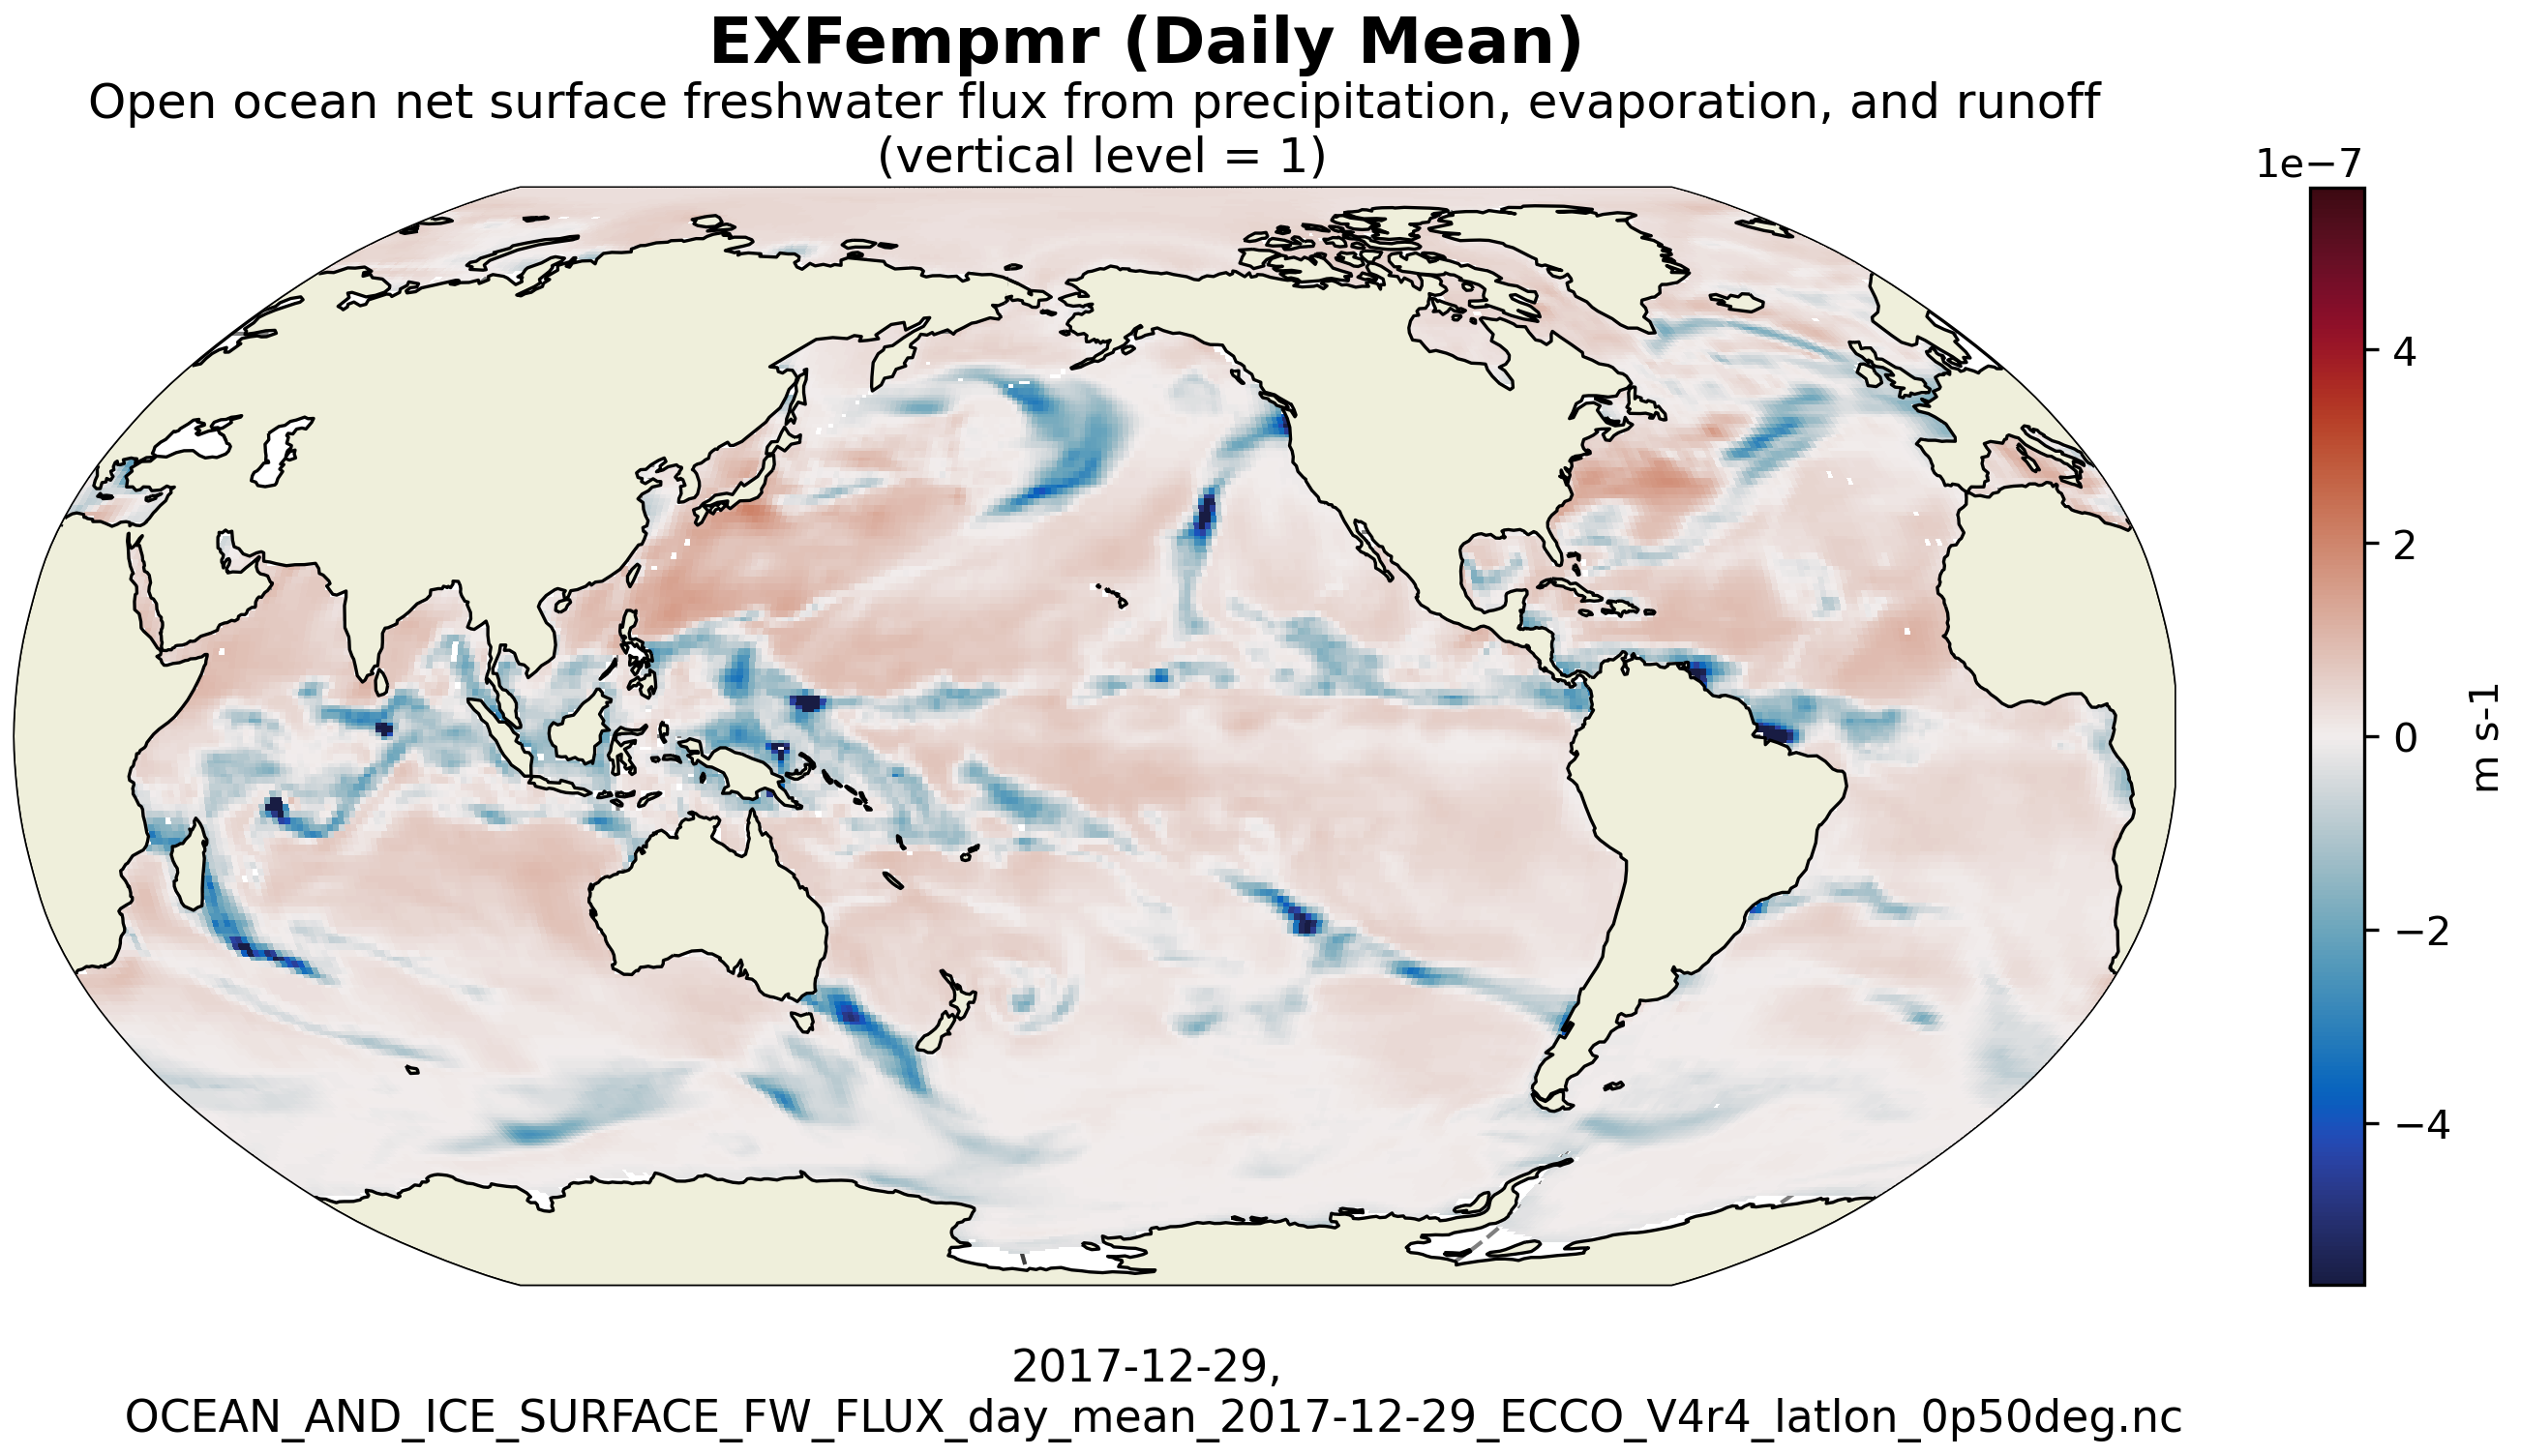
\includegraphics[scale=0.55]{../images/plots/v4r4/latlon_plots/Ocean_and_Sea-Ice_Surface_Freshwater_Fluxes/EXFempmr.png}
\caption{Dataset: OCEAN\_AND\_ICE\_SURFACE\_FW\_FLUX, Variable: EXFempmr}
\label{tab:table-OCEAN_AND_ICE_SURFACE_FW_FLUX_EXFempmr-Plot}
\end{figure}
\newpage
\pagebreak
\subsubsection{Latlon Variable: EXFevap}
\begin{longtable}{|m{0.06\textwidth}|m{0.3\textwidth}|m{0.45\textwidth}|m{0.12\textwidth}|}
\caption{Attributes description of the variable 'EXFevap' from OCEAN\_AND\_ICE\_SURFACE\_FW\_FLUX's  dataset.}
\label{tab:table-OCEAN_AND_ICE_SURFACE_FW_FLUX_EXFevap} \\ 
\hline \endhead \hline \endfoot
\rowcolor{lightgray} \textbf{Storage Type} & \textbf{Variable Name} & \textbf{Description} & \textbf{Unit} \\ \hline
float32 & EXFevap & Open ocean evaporation rate & m s-1 \\ \hline
\multicolumn{4}{|c|}{\cellcolor{lightgray}{\textbf{Description of the variable in Common Data language (CDL)}}} \\ \hline
\multicolumn{4}{|c|}{\fontfamily{lmtt}\selectfont{\makecell{\parbox{.95\textwidth}{\vspace*{0.25cm} \footnotesize{float32 EXFevap(time, latitude, longitude)\\
\hspace*{0.5cm}EXFevap: \_FillValue = 9.96921e+36\\
\hspace*{0.5cm}EXFevap: coordinates = time\\
\hspace*{0.5cm}EXFevap: coverage\_content\_type = modelResult\\
\hspace*{0.5cm}EXFevap: direction = >0 increases salinity (SALT)\\
\hspace*{0.5cm}EXFevap: long\_name = Open ocean evaporation rate\\
\hspace*{0.5cm}EXFevap: standard\_name = lwe water evaporation rate\\
\hspace*{0.5cm}EXFevap: units = m s-1\\
\hspace*{0.5cm}EXFevap: valid\_max = 7.090054623404285e-07\\
\hspace*{0.5cm}EXFevap: valid\_min = -1.0958113705328287e-07\\
}}}}} \\ \hline
\rowcolor{lightgray} \multicolumn{4}{|c|}{\textbf{Comments}} \\ \hline
\multicolumn{4}{|p{1\textwidth}|}{\footnotesize{{Evaporation rate per unit area of open water (not covered by sea-ice). note: calculated using the bulk formula following large and yeager (2004) ncar/tn-460+str.}}} \\ \hline
\end{longtable}

\begin{figure}[H]
\centering
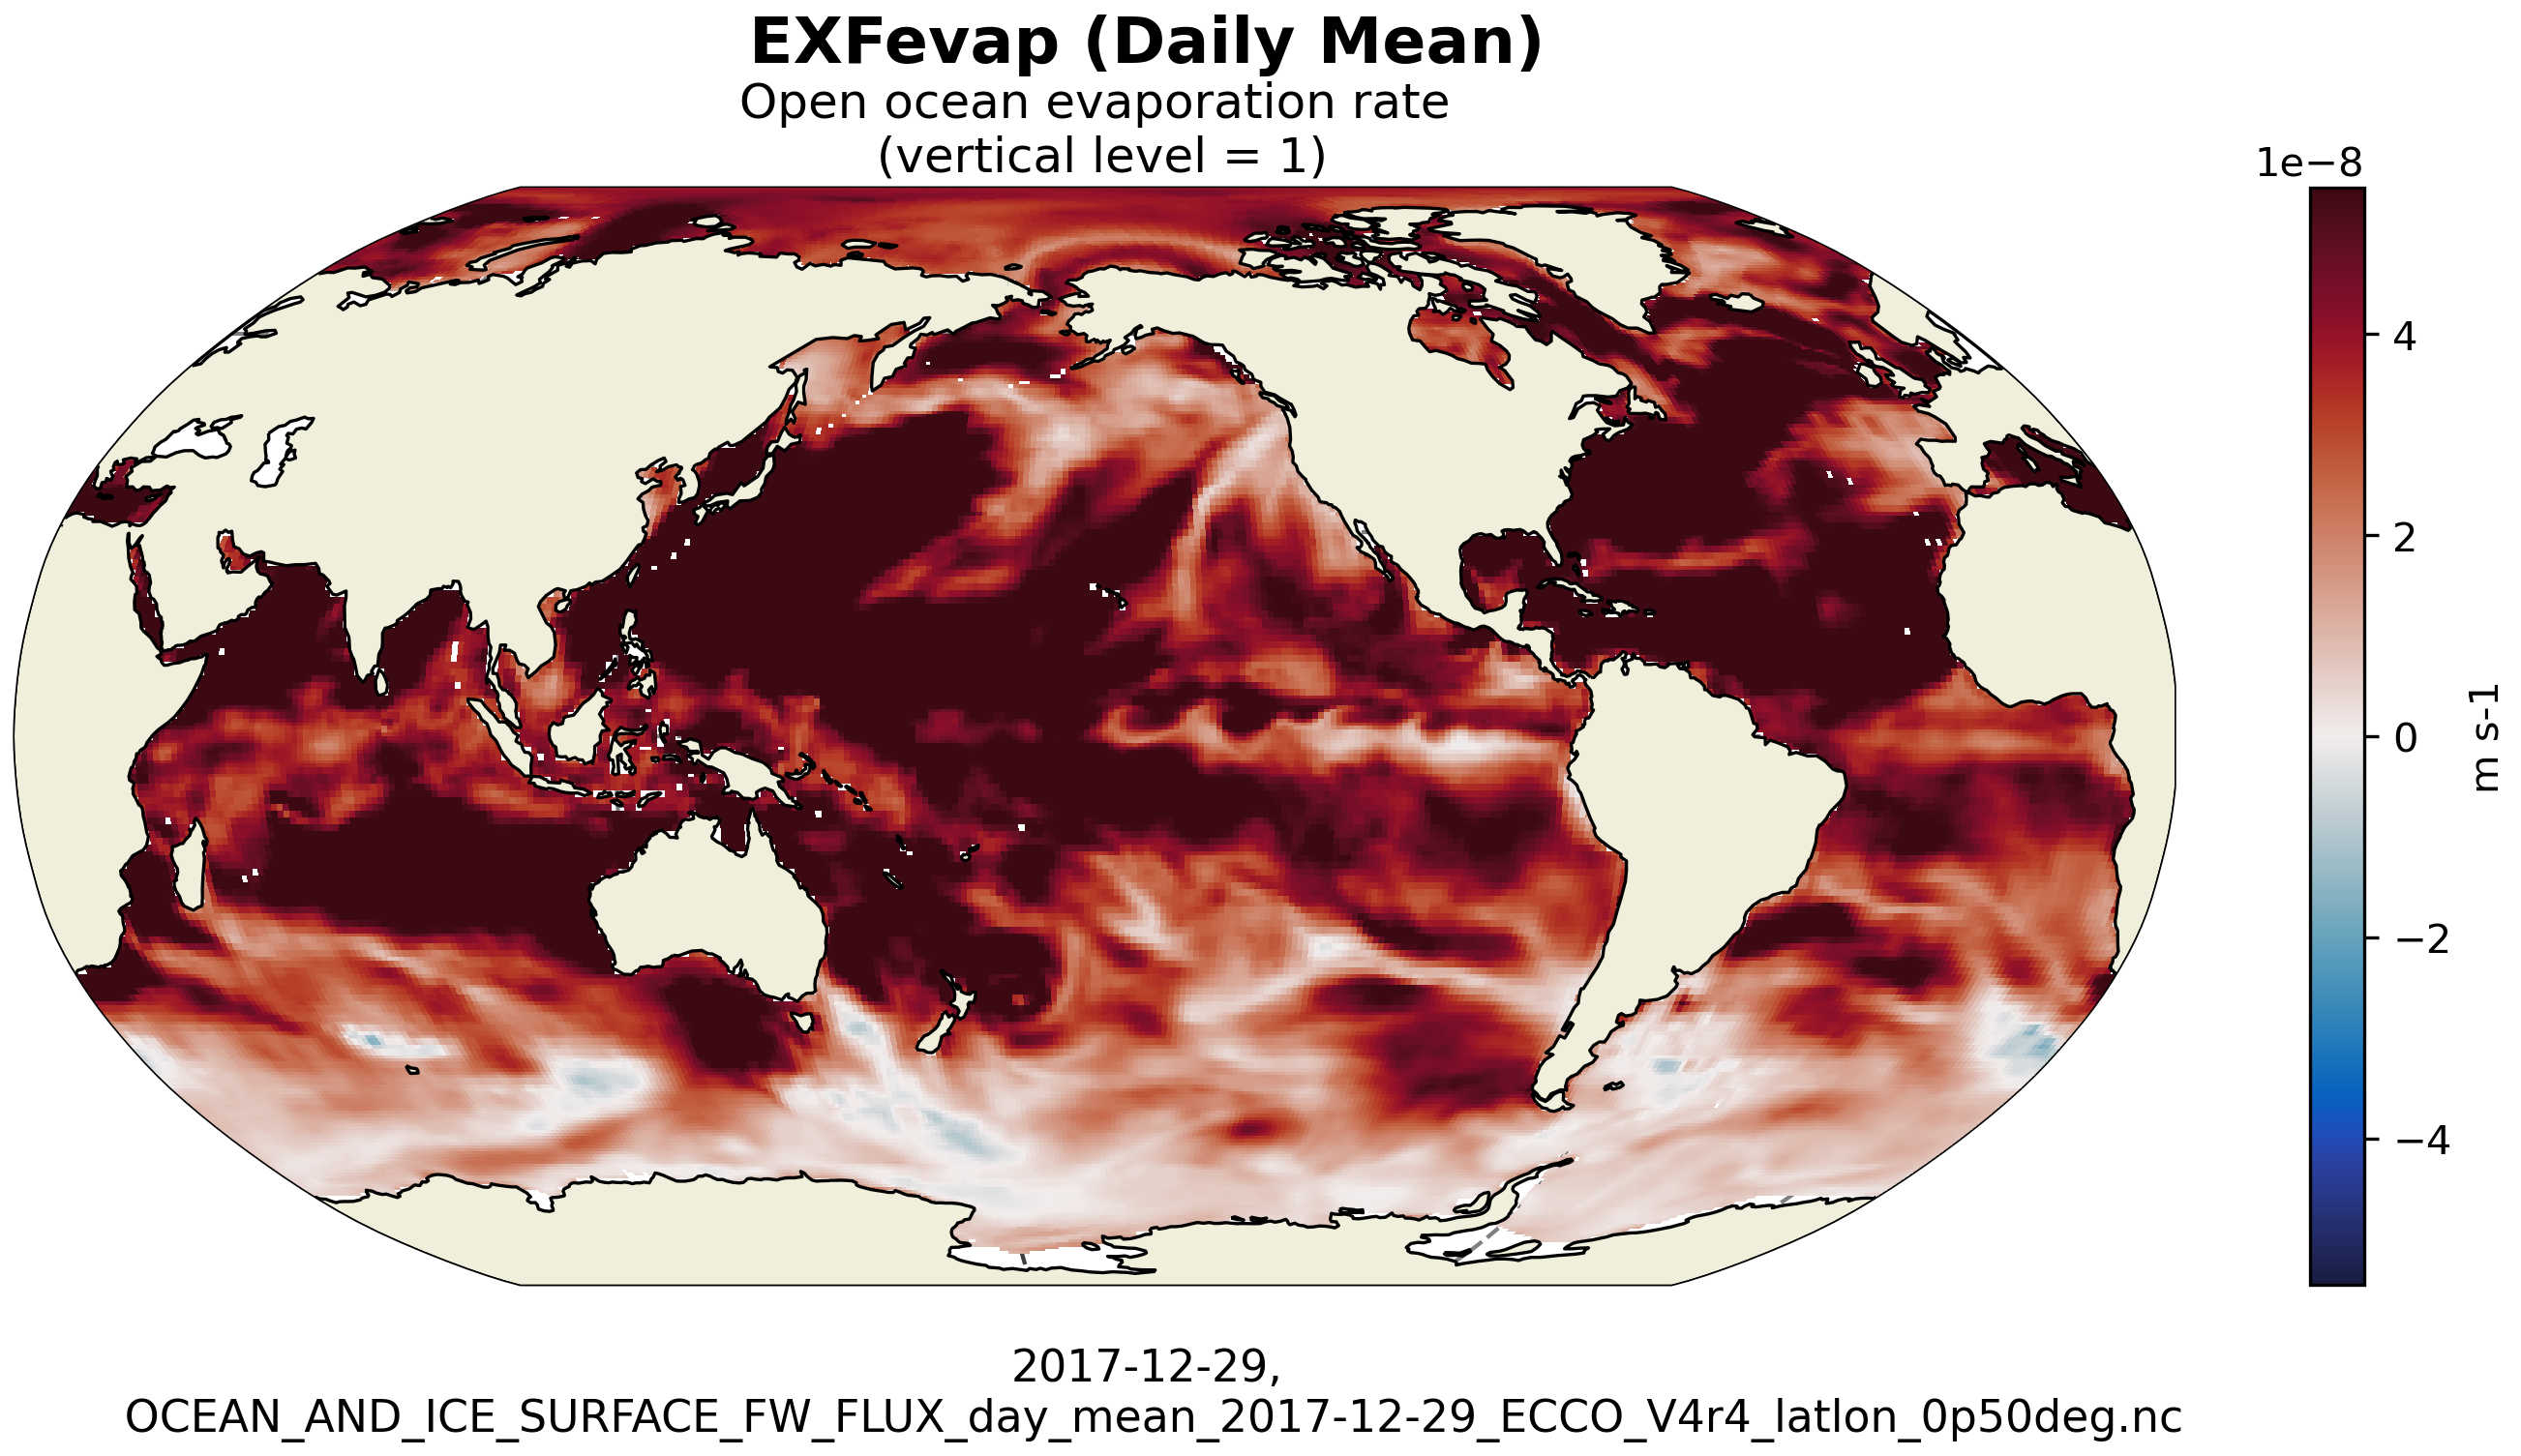
\includegraphics[scale=0.55]{../images/plots/v4r4/latlon_plots/Ocean_and_Sea-Ice_Surface_Freshwater_Fluxes/EXFevap.png}
\caption{Dataset: OCEAN\_AND\_ICE\_SURFACE\_FW\_FLUX, Variable: EXFevap}
\label{tab:table-OCEAN_AND_ICE_SURFACE_FW_FLUX_EXFevap-Plot}
\end{figure}
\newpage
\pagebreak
\subsubsection{Latlon Variable: EXFpreci}
\begin{longtable}{|m{0.06\textwidth}|m{0.3\textwidth}|m{0.45\textwidth}|m{0.12\textwidth}|}
\caption{Attributes description of the variable 'EXFpreci' from OCEAN\_AND\_ICE\_SURFACE\_FW\_FLUX's  dataset.}
\label{tab:table-OCEAN_AND_ICE_SURFACE_FW_FLUX_EXFpreci} \\ 
\hline \endhead \hline \endfoot
\rowcolor{lightgray} \textbf{Storage Type} & \textbf{Variable Name} & \textbf{Description} & \textbf{Unit} \\ \hline
float32 & EXFpreci & Precipitation rate & m s-1 \\ \hline
\multicolumn{4}{|c|}{\cellcolor{lightgray}{\textbf{Description of the variable in Common Data language (CDL)}}} \\ \hline
\multicolumn{4}{|c|}{\fontfamily{lmtt}\selectfont{\makecell{\parbox{.95\textwidth}{\vspace*{0.25cm} \footnotesize{float32 EXFpreci(time, latitude, longitude)\\
\hspace*{0.5cm}EXFpreci: \_FillValue = 9.96921e+36\\
\hspace*{0.5cm}EXFpreci: coordinates = time\\
\hspace*{0.5cm}EXFpreci: coverage\_content\_type = modelResult\\
\hspace*{0.5cm}EXFpreci: direction = >0 increases salinity (SALT)\\
\hspace*{0.5cm}EXFpreci: long\_name = Precipitation rate\\
\hspace*{0.5cm}EXFpreci: standard\_name = lwe precipitation rate\\
\hspace*{0.5cm}EXFpreci: units = m s-1\\
\hspace*{0.5cm}EXFpreci: valid\_max = 8.317776519106701e-06\\
\hspace*{0.5cm}EXFpreci: valid\_min = -1.4860395936011628e-07\\
}}}}} \\ \hline
\rowcolor{lightgray} \multicolumn{4}{|c|}{\textbf{Comments}} \\ \hline
\multicolumn{4}{|p{1\textwidth}|}{\footnotesize{{Precipitation rate. note: sum of era-interim precipitation and the control adjustment from ocean state estimation.}}} \\ \hline
\end{longtable}

\begin{figure}[H]
\centering
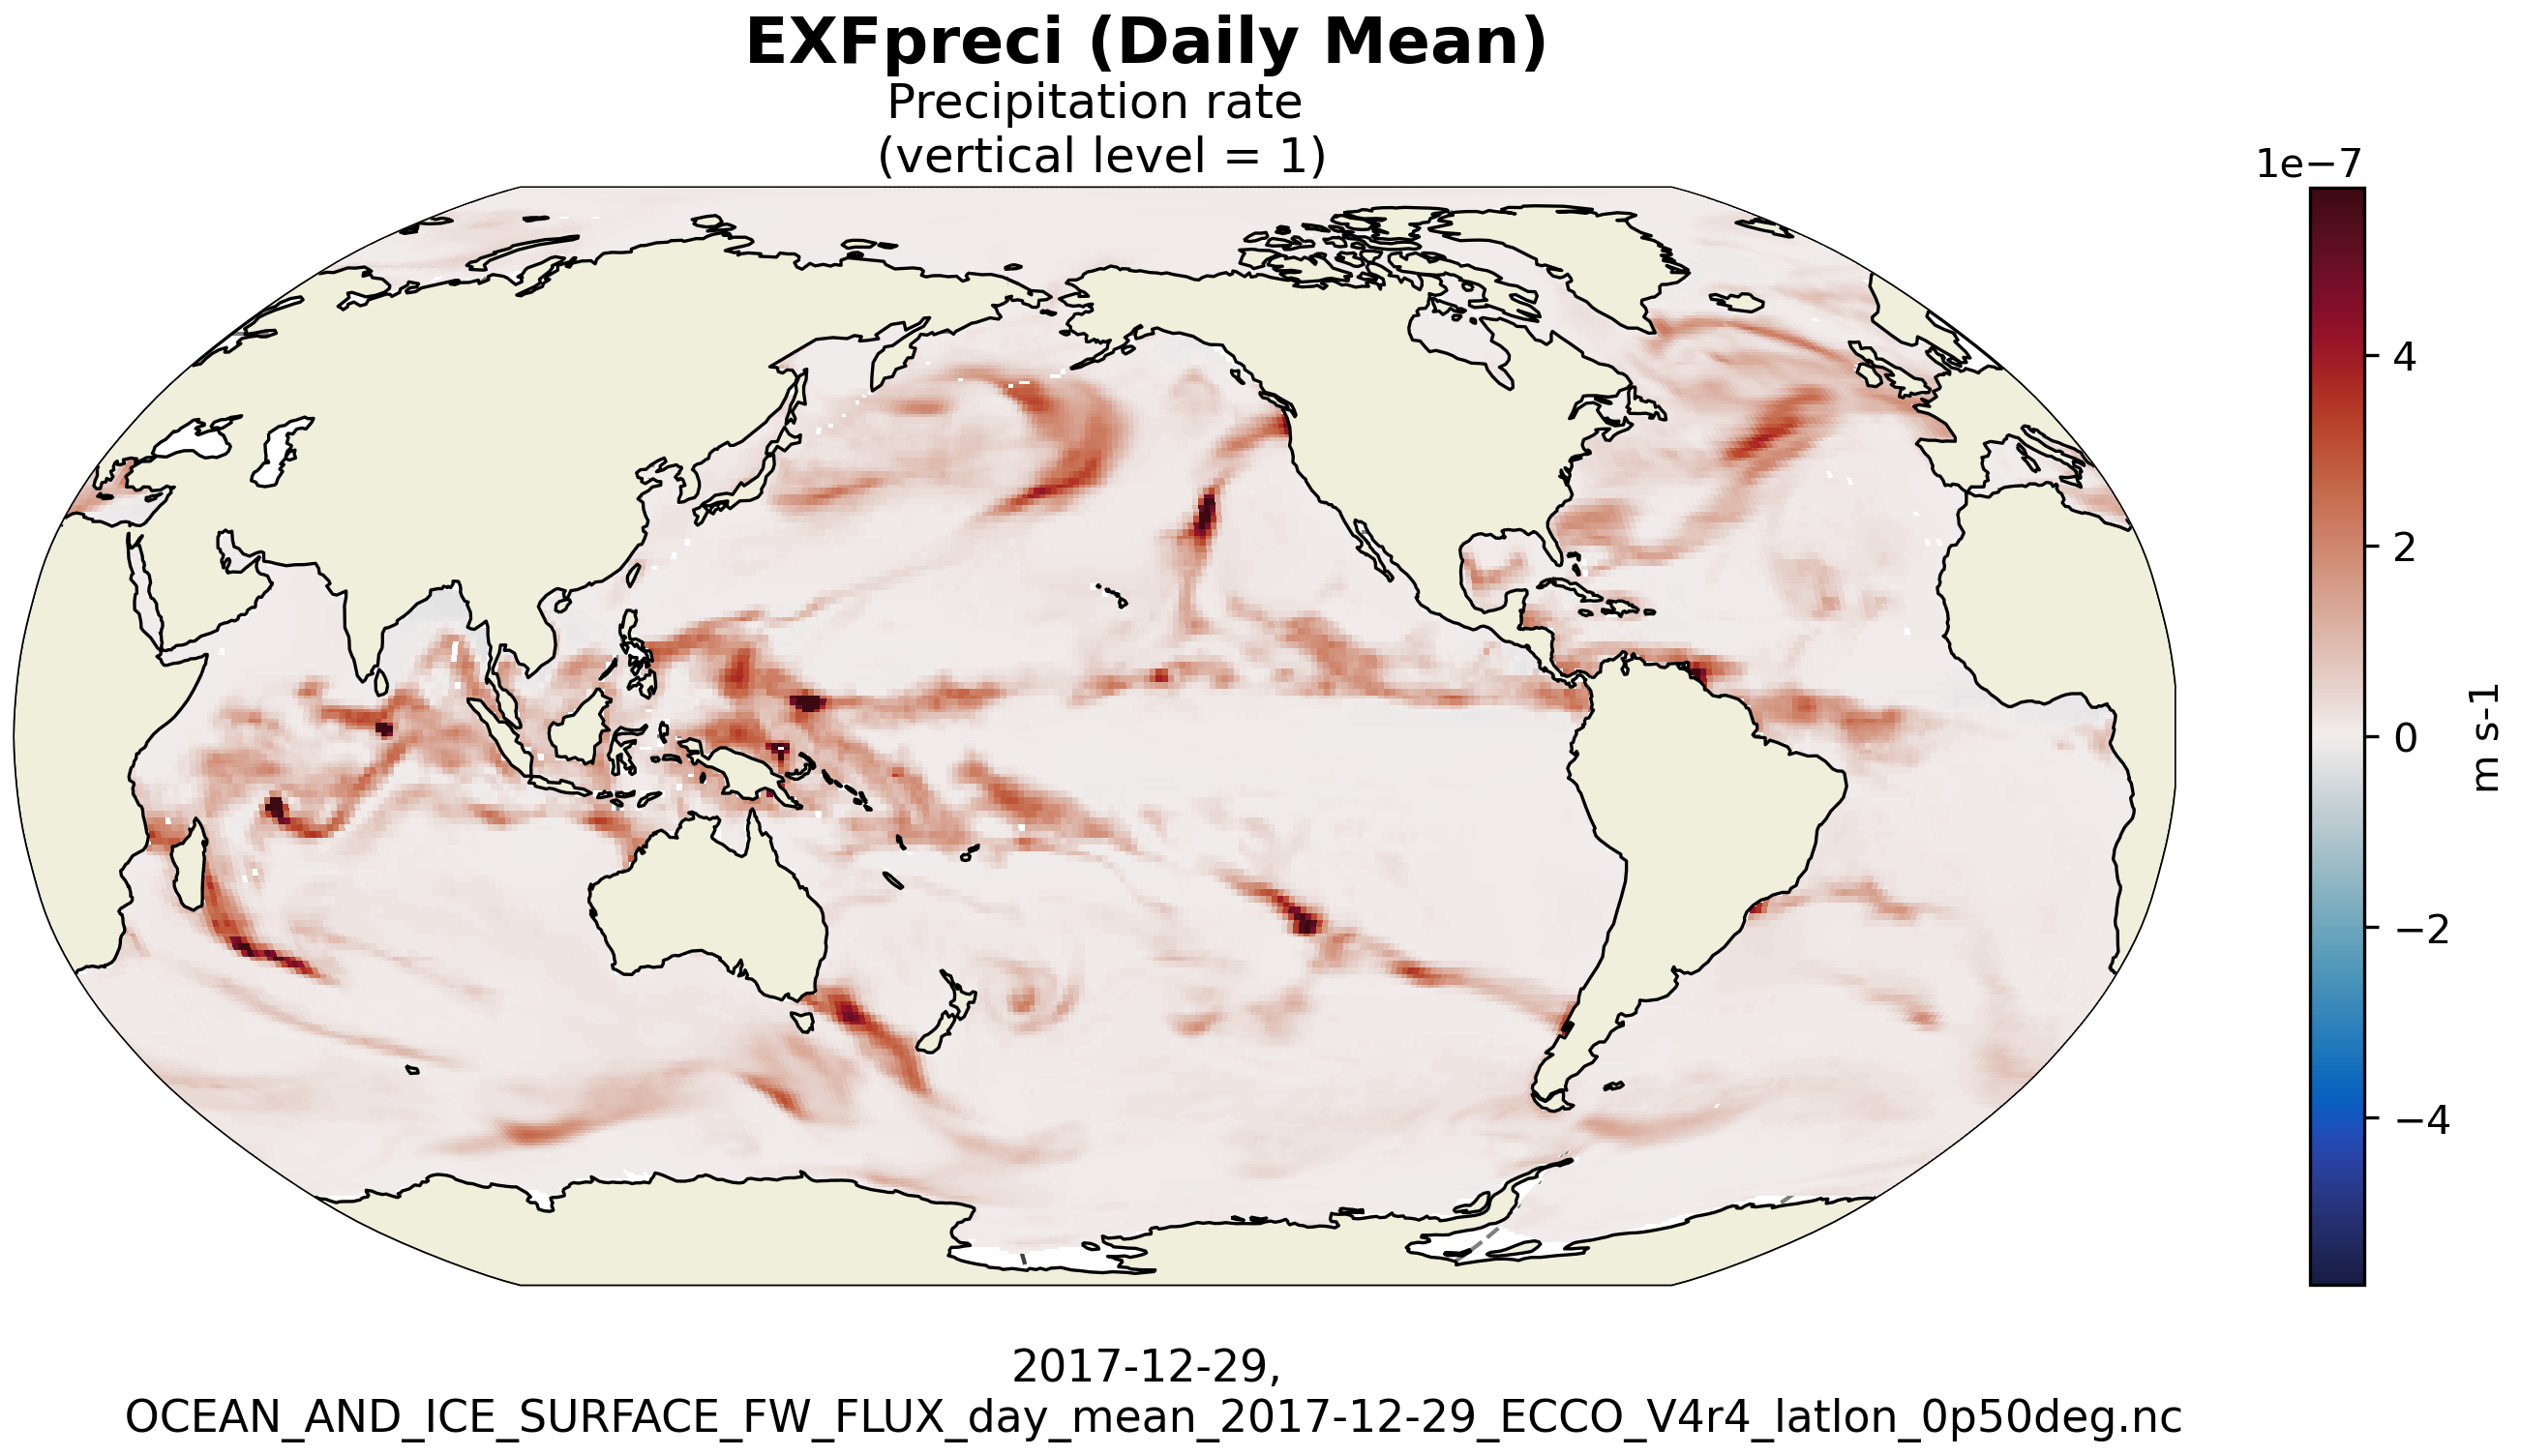
\includegraphics[scale=0.55]{../images/plots/v4r4/latlon_plots/Ocean_and_Sea-Ice_Surface_Freshwater_Fluxes/EXFpreci.png}
\caption{Dataset: OCEAN\_AND\_ICE\_SURFACE\_FW\_FLUX, Variable: EXFpreci}
\label{tab:table-OCEAN_AND_ICE_SURFACE_FW_FLUX_EXFpreci-Plot}
\end{figure}
\newpage
\pagebreak
\subsubsection{Latlon Variable: EXFroff}
\begin{longtable}{|m{0.06\textwidth}|m{0.3\textwidth}|m{0.45\textwidth}|m{0.12\textwidth}|}
\caption{Attributes description of the variable 'EXFroff' from OCEAN\_AND\_ICE\_SURFACE\_FW\_FLUX's  dataset.}
\label{tab:table-OCEAN_AND_ICE_SURFACE_FW_FLUX_EXFroff} \\ 
\hline \endhead \hline \endfoot
\rowcolor{lightgray} \textbf{Storage Type} & \textbf{Variable Name} & \textbf{Description} & \textbf{Unit} \\ \hline
float32 & EXFroff & River runoff & m s-1 \\ \hline
\multicolumn{4}{|c|}{\cellcolor{lightgray}{\textbf{Description of the variable in Common Data language (CDL)}}} \\ \hline
\multicolumn{4}{|c|}{\fontfamily{lmtt}\selectfont{\makecell{\parbox{.95\textwidth}{\vspace*{0.25cm} \footnotesize{float32 EXFroff(time, latitude, longitude)\\
\hspace*{0.5cm}EXFroff: \_FillValue = 9.96921e+36\\
\hspace*{0.5cm}EXFroff: coordinates = time\\
\hspace*{0.5cm}EXFroff: coverage\_content\_type = modelResult\\
\hspace*{0.5cm}EXFroff: direction = >0 increases salinity (SALT)\\
\hspace*{0.5cm}EXFroff: long\_name = River runoff\\
\hspace*{0.5cm}EXFroff: standard\_name = surface runoff flux\\
\hspace*{0.5cm}EXFroff: units = m s-1\\
\hspace*{0.5cm}EXFroff: valid\_max = 4.185612397122895e-06\\
\hspace*{0.5cm}EXFroff: valid\_min = 0.0\\
}}}}} \\ \hline
\rowcolor{lightgray} \multicolumn{4}{|c|}{\textbf{Comments}} \\ \hline
\multicolumn{4}{|p{1\textwidth}|}{\footnotesize{{River runoff freshwater flux. note: not adjusted by the optimization.}}} \\ \hline
\end{longtable}

\begin{figure}[H]
\centering
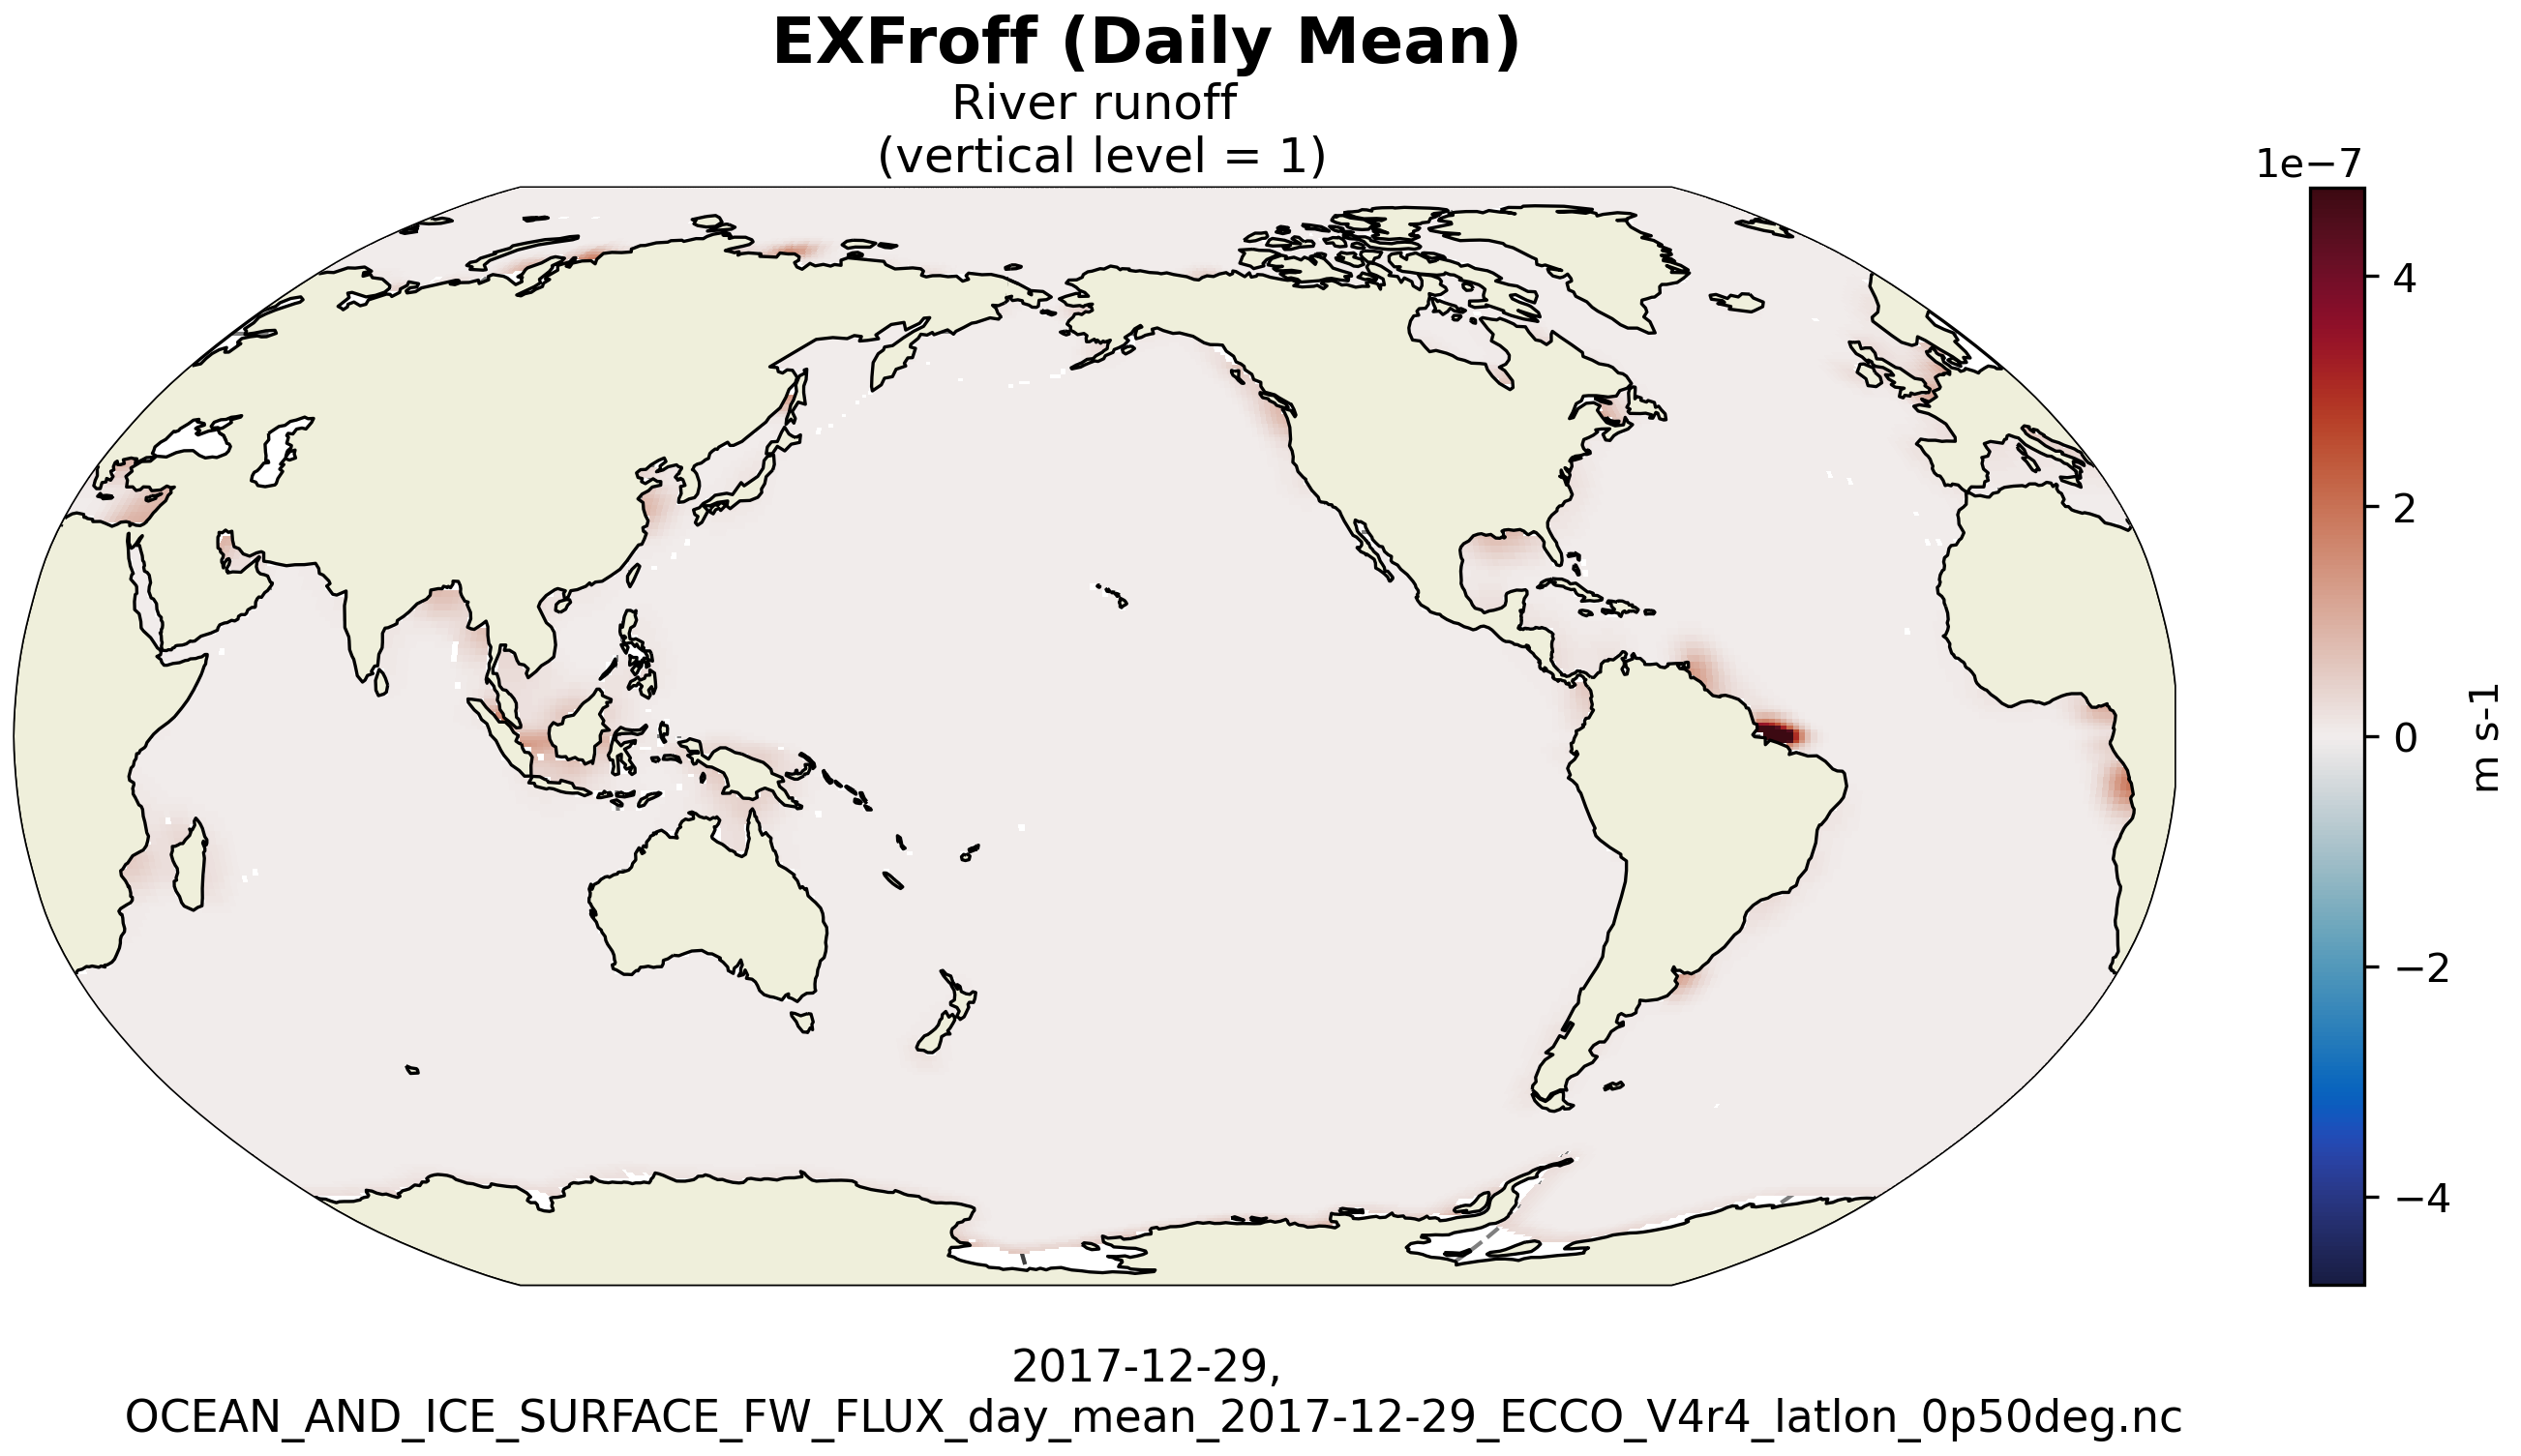
\includegraphics[scale=0.55]{../images/plots/v4r4/latlon_plots/Ocean_and_Sea-Ice_Surface_Freshwater_Fluxes/EXFroff.png}
\caption{Dataset: OCEAN\_AND\_ICE\_SURFACE\_FW\_FLUX, Variable: EXFroff}
\label{tab:table-OCEAN_AND_ICE_SURFACE_FW_FLUX_EXFroff-Plot}
\end{figure}
\newpage
\pagebreak
\subsubsection{Latlon Variable: SFLUX}
\begin{longtable}{|m{0.06\textwidth}|m{0.3\textwidth}|m{0.45\textwidth}|m{0.12\textwidth}|}
\caption{Attributes description of the variable 'SFLUX' from OCEAN\_AND\_ICE\_SURFACE\_FW\_FLUX's  dataset.}
\label{tab:table-OCEAN_AND_ICE_SURFACE_FW_FLUX_SFLUX} \\ 
\hline \endhead \hline \endfoot
\rowcolor{lightgray} \textbf{Storage Type} & \textbf{Variable Name} & \textbf{Description} & \textbf{Unit} \\ \hline
float32 & SFLUX & Rate of change of total ocean salinity per m2 accounting for mass fluxes. & g m-2 s-1 \\ \hline
\multicolumn{4}{|c|}{\cellcolor{lightgray}{\textbf{Description of the variable in Common Data language (CDL)}}} \\ \hline
\multicolumn{4}{|c|}{\fontfamily{lmtt}\selectfont{\makecell{\parbox{.95\textwidth}{\vspace*{0.25cm} \footnotesize{float32 SFLUX(time, latitude, longitude)\\
\hspace*{0.5cm}SFLUX: \_FillValue = 9.96921e+36\\
\hspace*{0.5cm}SFLUX: coordinates = time\\
\hspace*{0.5cm}SFLUX: coverage\_content\_type = modelResult\\
\hspace*{0.5cm}SFLUX: direction = >0 increases salinity (SALT)\\
\hspace*{0.5cm}SFLUX: long\_name = Rate of change of total ocean salinity per m2 accounting for mass fluxes.\\
\hspace*{0.5cm}SFLUX: units = g m-2 s-1\\
\hspace*{0.5cm}SFLUX: valid\_max = 0.010570422746241093\\
\hspace*{0.5cm}SFLUX: valid\_min = -0.06244903802871704\\
}}}}} \\ \hline
\rowcolor{lightgray} \multicolumn{4}{|c|}{\textbf{Comments}} \\ \hline
\multicolumn{4}{|p{1\textwidth}|}{\footnotesize{{The rate of change of total ocean salinity due to freshwater fluxes across the liquid surface and the addition or removal of mass. note: the global area integral of sflux matches the time-derivative of total ocean salinity (psu s-1). unlike ocefwflx, sflux includes the contribution to the total ocean salinity from changing ocean mass (e.g. from the addition or removal of freshwater in ocefwflx). }}} \\ \hline
\end{longtable}

\begin{figure}[H]
\centering
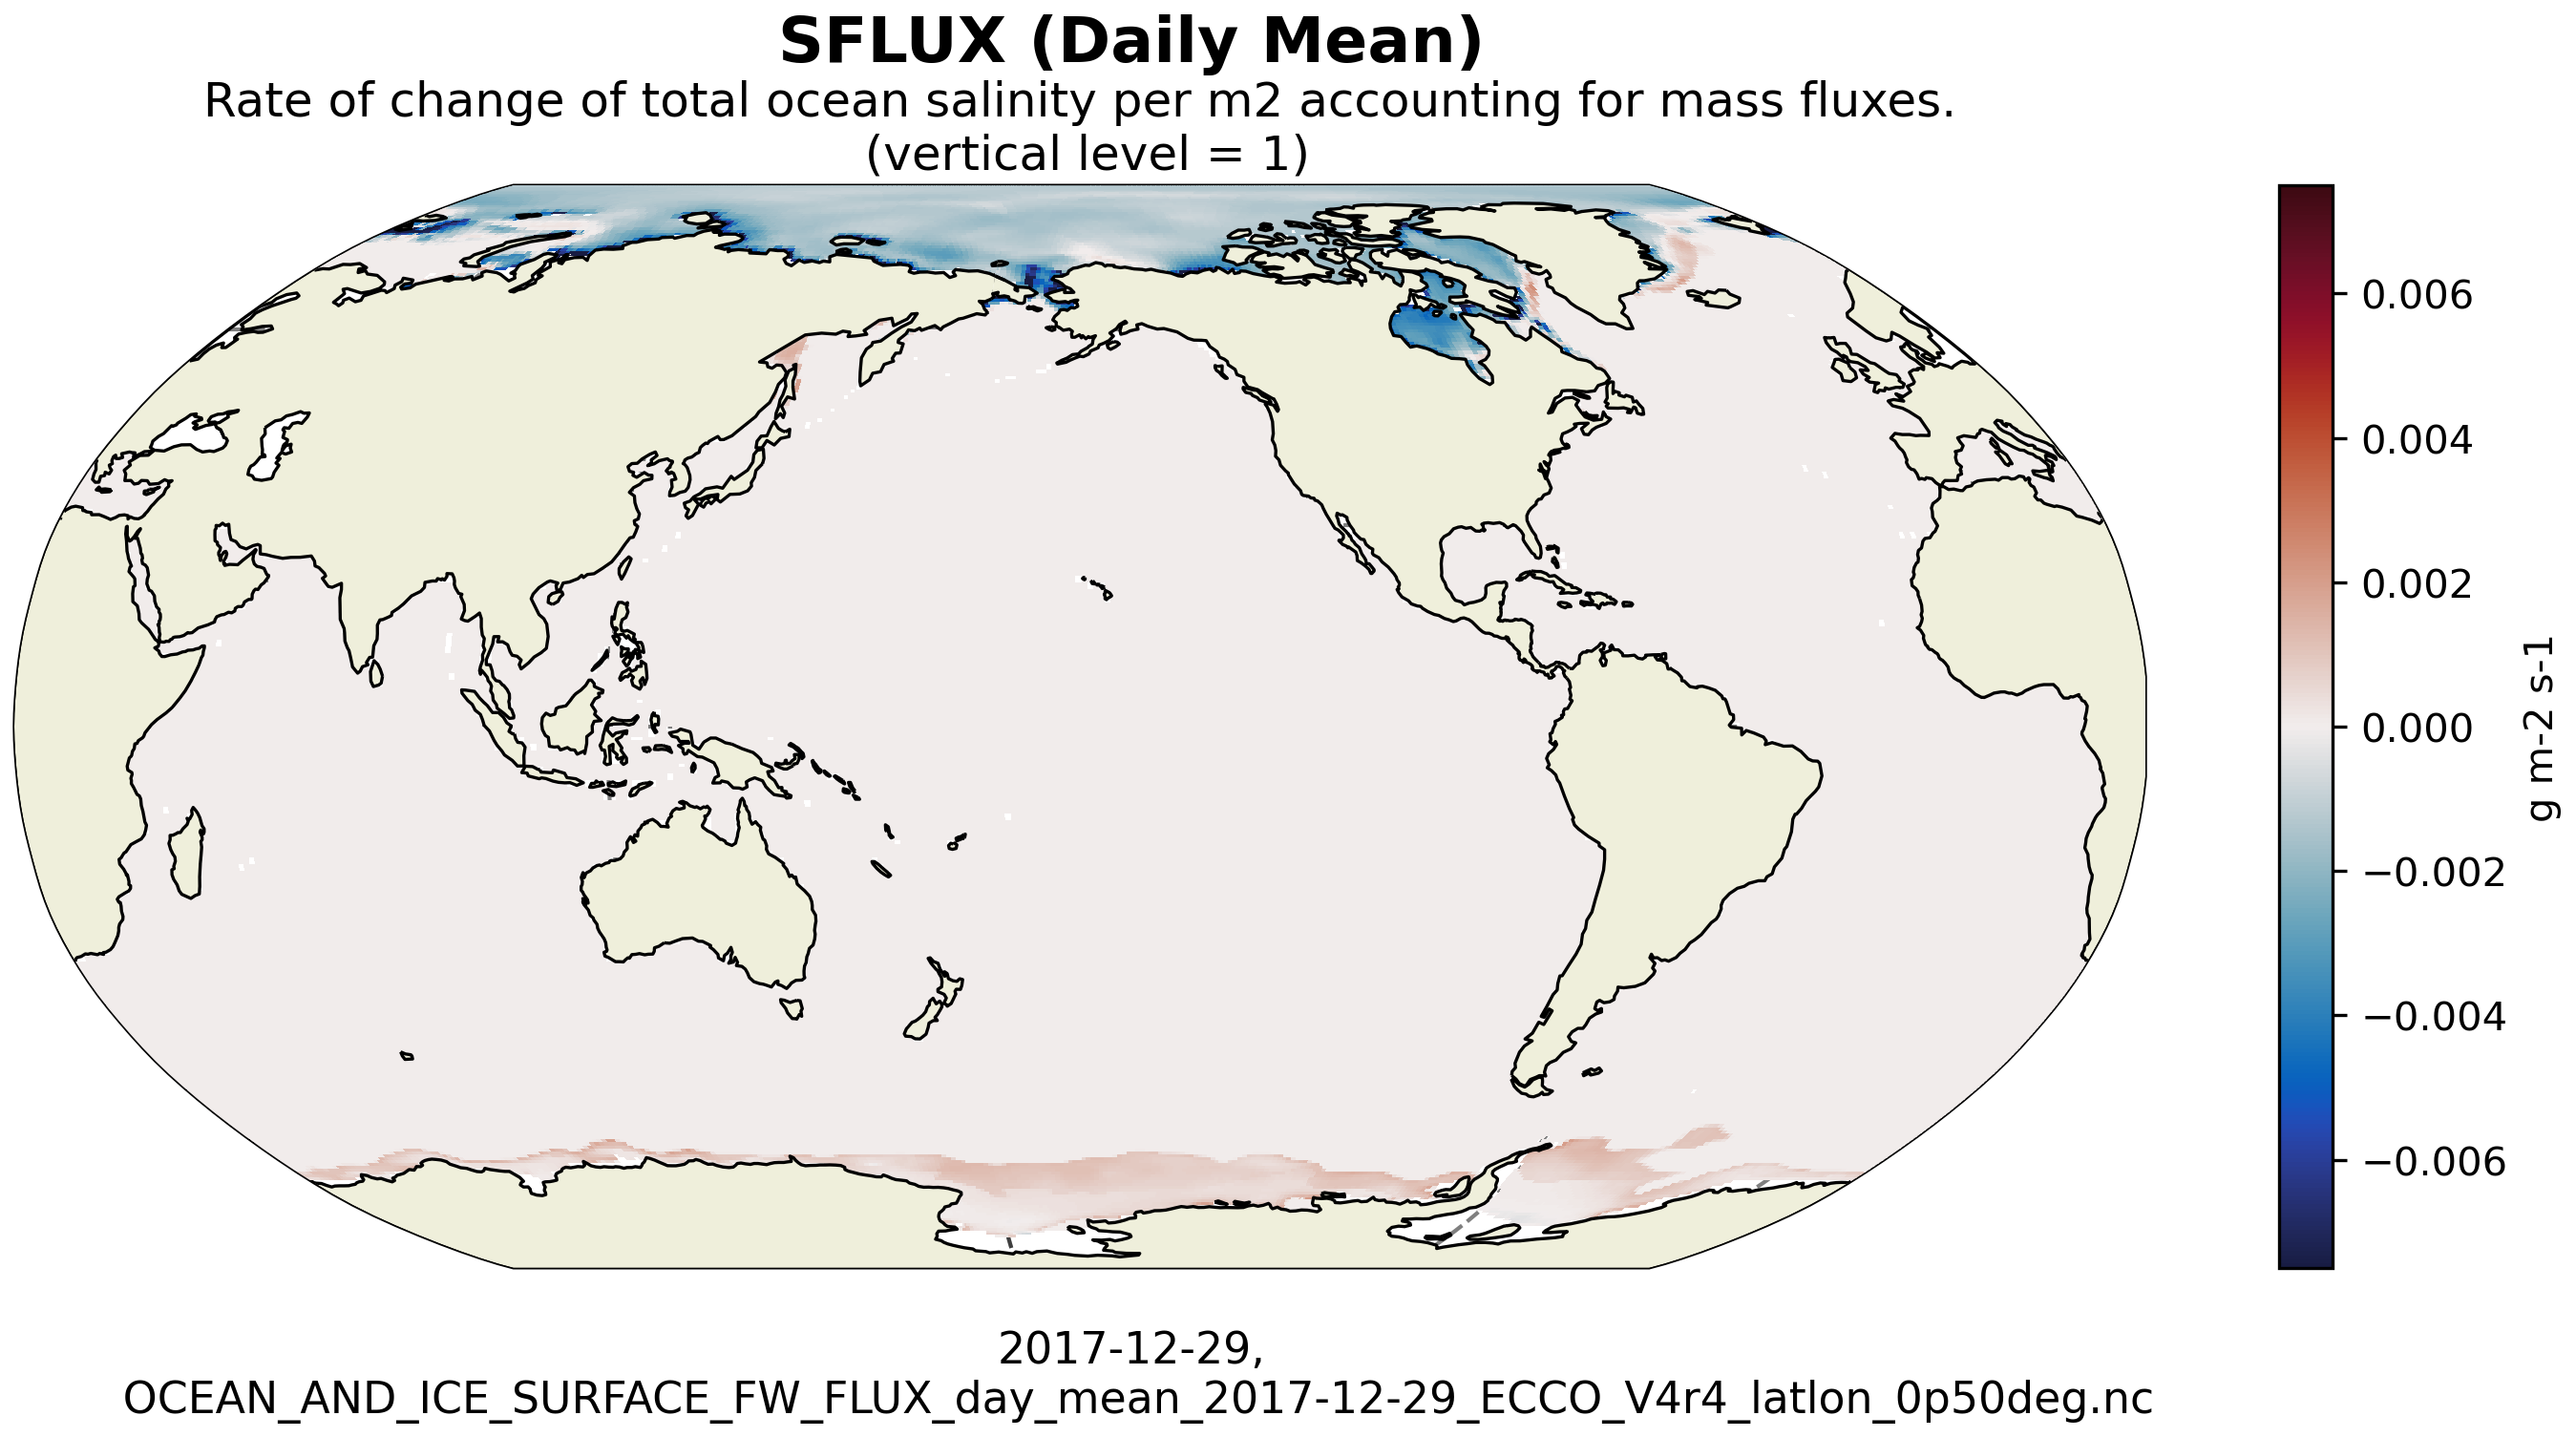
\includegraphics[scale=0.55]{../images/plots/v4r4/latlon_plots/Ocean_and_Sea-Ice_Surface_Freshwater_Fluxes/SFLUX.png}
\caption{Dataset: OCEAN\_AND\_ICE\_SURFACE\_FW\_FLUX, Variable: SFLUX}
\label{tab:table-OCEAN_AND_ICE_SURFACE_FW_FLUX_SFLUX-Plot}
\end{figure}
\newpage
\pagebreak
\subsubsection{Latlon Variable: SIacSubl}
\begin{longtable}{|m{0.06\textwidth}|m{0.3\textwidth}|m{0.45\textwidth}|m{0.12\textwidth}|}
\caption{Attributes description of the variable 'SIacSubl' from OCEAN\_AND\_ICE\_SURFACE\_FW\_FLUX's  dataset.}
\label{tab:table-OCEAN_AND_ICE_SURFACE_FW_FLUX_SIacSubl} \\ 
\hline \endhead \hline \endfoot
\rowcolor{lightgray} \textbf{Storage Type} & \textbf{Variable Name} & \textbf{Description} & \textbf{Unit} \\ \hline
float32 & SIacSubl & Freshwater flux to the atmosphere due to sublimation-deposition of snow or ice & kg m-2 s-1 \\ \hline
\multicolumn{4}{|c|}{\cellcolor{lightgray}{\textbf{Description of the variable in Common Data language (CDL)}}} \\ \hline
\multicolumn{4}{|c|}{\fontfamily{lmtt}\selectfont{\makecell{\parbox{.95\textwidth}{\vspace*{0.25cm} \footnotesize{float32 SIacSubl(time, latitude, longitude)\\
\hspace*{0.5cm}SIacSubl: \_FillValue = 9.96921e+36\\
\hspace*{0.5cm}SIacSubl: coordinates = time\\
\hspace*{0.5cm}SIacSubl: coverage\_content\_type = modelResult\\
\hspace*{0.5cm}SIacSubl: direction = >0 decreases snow or sea-ice thickness (HSNOW or HEFF)\\
\hspace*{0.5cm}SIacSubl: long\_name = Freshwater flux to the atmosphere due to sublimation-deposition of snow or ice\\
\hspace*{0.5cm}SIacSubl: standard\_name = water sublimation flux\\
\hspace*{0.5cm}SIacSubl: units = kg m-2 s-1\\
\hspace*{0.5cm}SIacSubl: valid\_max = 7.735946564935148e-05\\
\hspace*{0.5cm}SIacSubl: valid\_min = 0.0\\
}}}}} \\ \hline
\rowcolor{lightgray} \multicolumn{4}{|c|}{\textbf{Comments}} \\ \hline
\multicolumn{4}{|p{1\textwidth}|}{\footnotesize{{Freshwater flux to the atmosphere due to sublimation-deposition of snow or ice. positive values imply sublimation from ice/snow to vapor, negative values imply deposition from atmospheric moisture}}} \\ \hline
\end{longtable}

\begin{figure}[H]
\centering
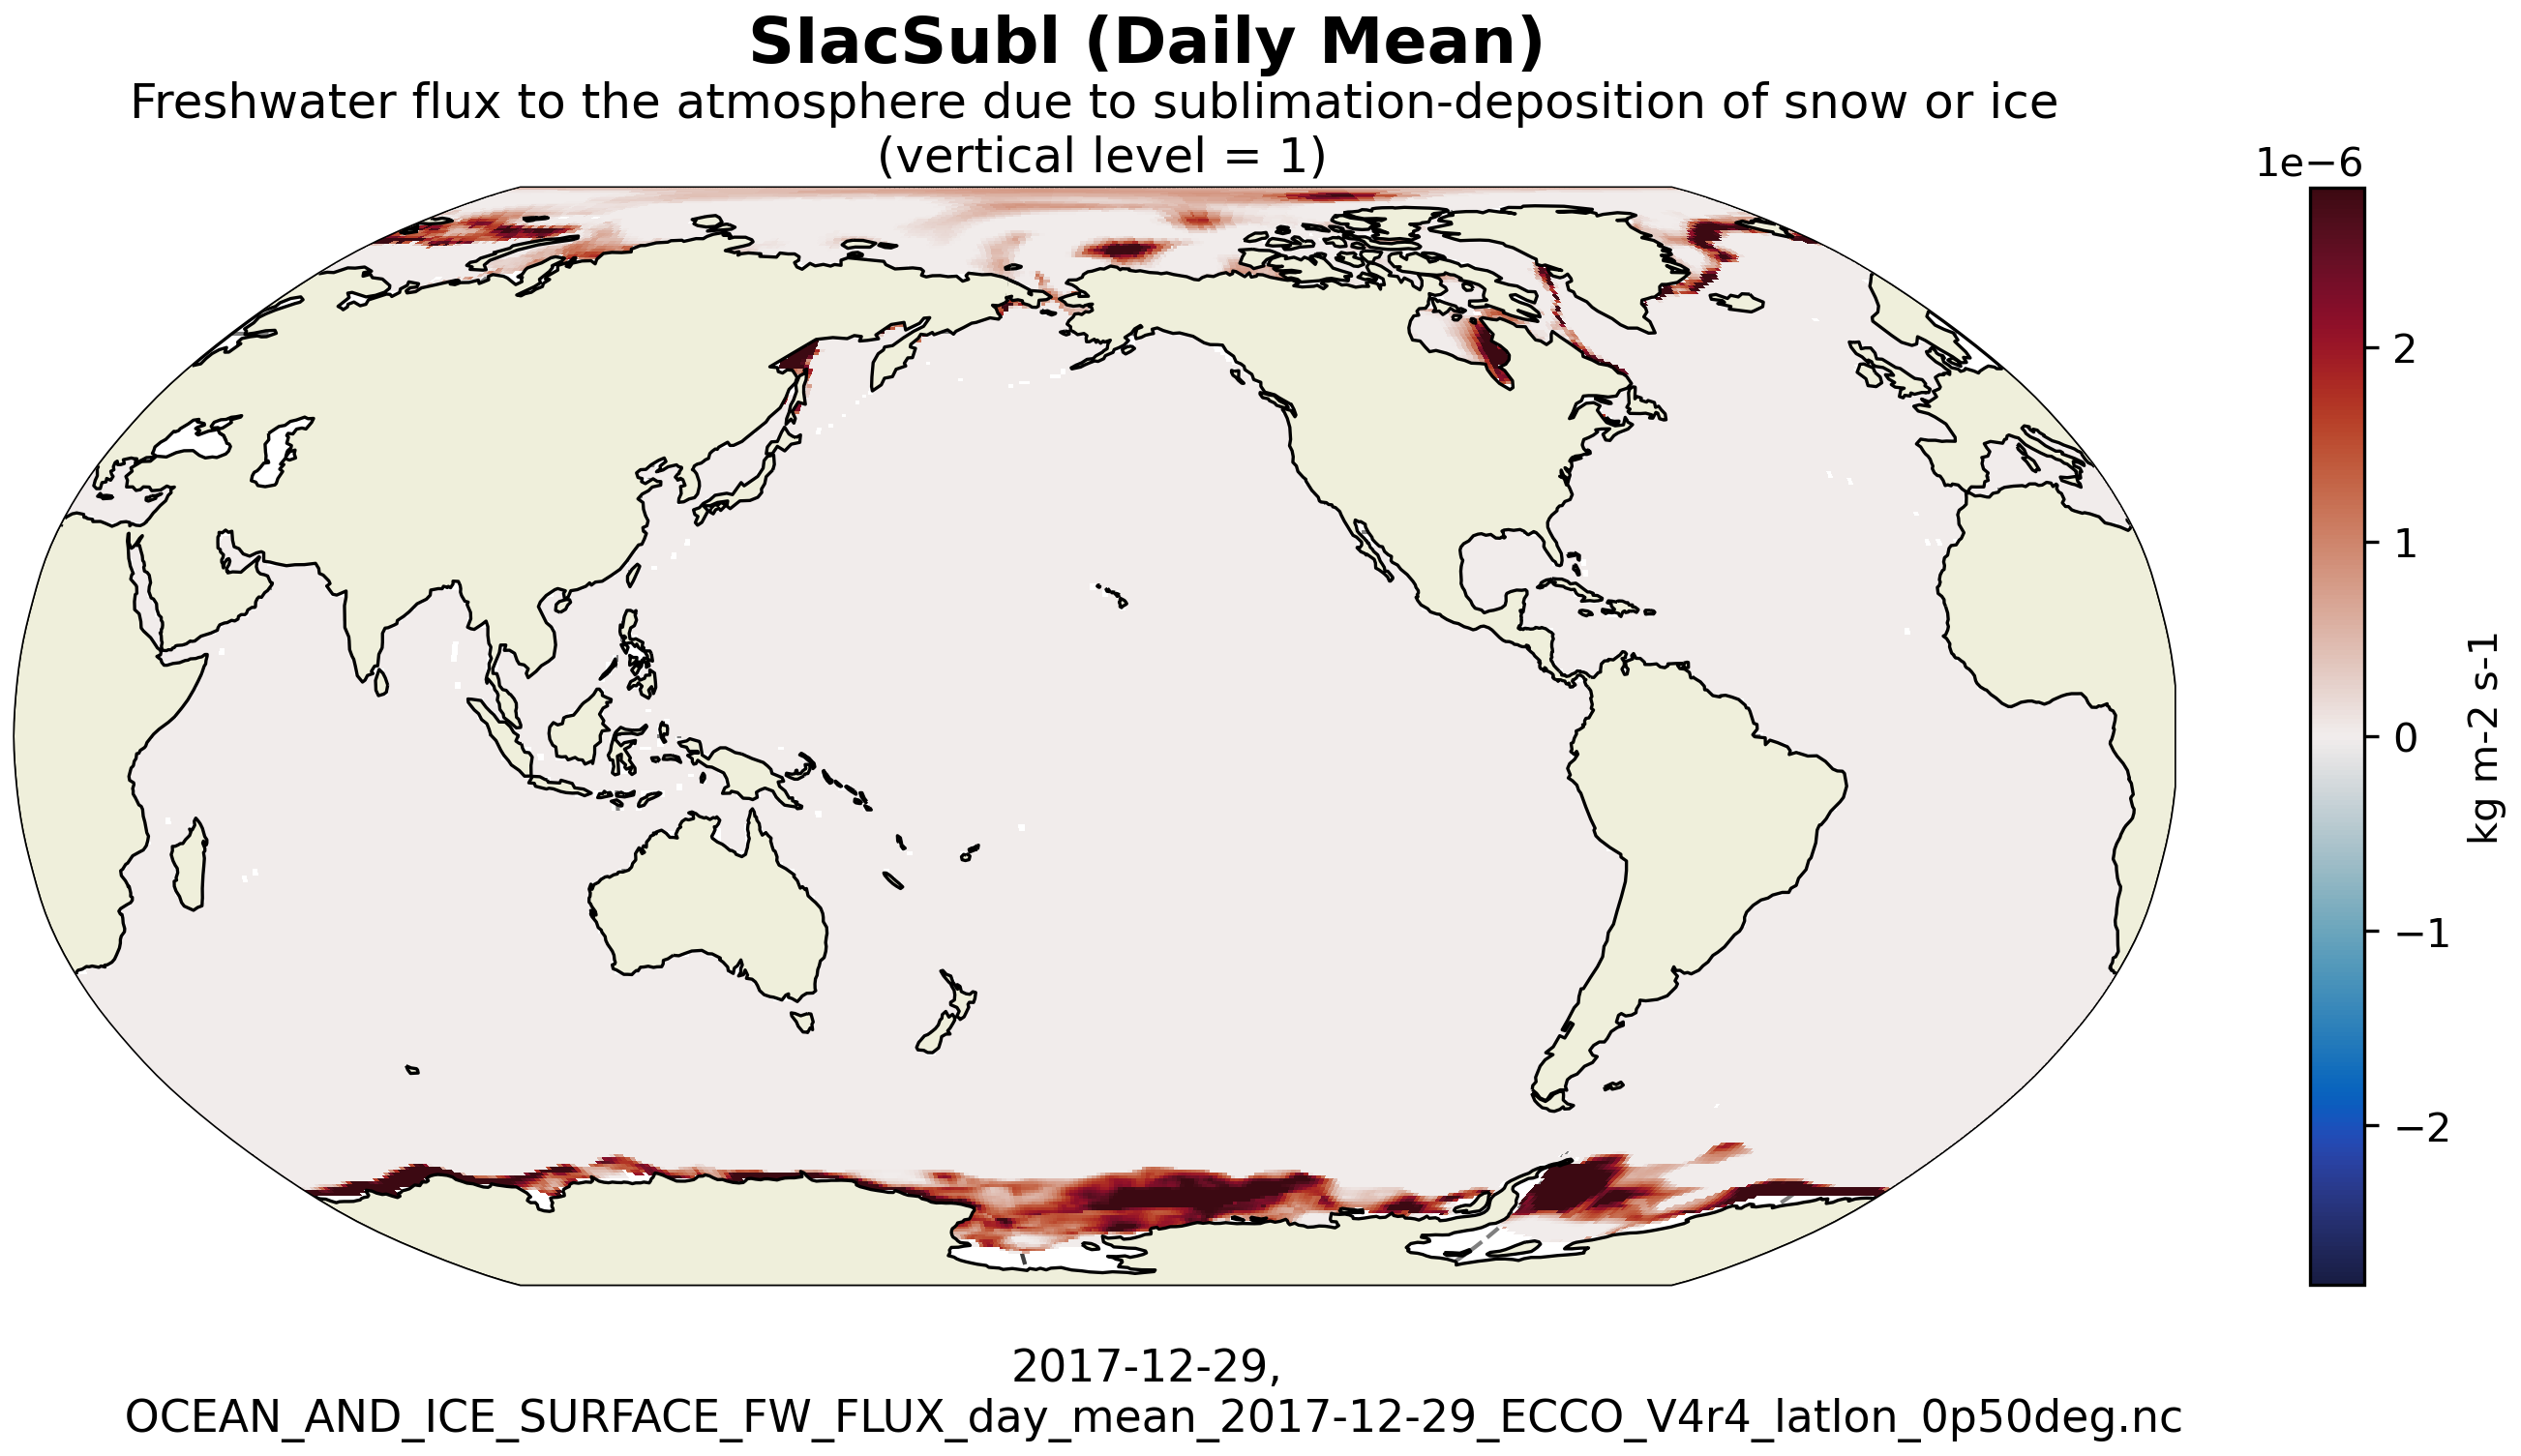
\includegraphics[scale=0.55]{../images/plots/v4r4/latlon_plots/Ocean_and_Sea-Ice_Surface_Freshwater_Fluxes/SIacSubl.png}
\caption{Dataset: OCEAN\_AND\_ICE\_SURFACE\_FW\_FLUX, Variable: SIacSubl}
\label{tab:table-OCEAN_AND_ICE_SURFACE_FW_FLUX_SIacSubl-Plot}
\end{figure}
\newpage
\pagebreak
\subsubsection{Latlon Variable: SIatmFW}
\begin{longtable}{|m{0.06\textwidth}|m{0.3\textwidth}|m{0.45\textwidth}|m{0.12\textwidth}|}
\caption{Attributes description of the variable 'SIatmFW' from OCEAN\_AND\_ICE\_SURFACE\_FW\_FLUX's  dataset.}
\label{tab:table-OCEAN_AND_ICE_SURFACE_FW_FLUX_SIatmFW} \\ 
\hline \endhead \hline \endfoot
\rowcolor{lightgray} \textbf{Storage Type} & \textbf{Variable Name} & \textbf{Description} & \textbf{Unit} \\ \hline
float32 & SIatmFW & Net freshwater flux into the open ocean, sea-ice, and snow & kg m-2 s-1 \\ \hline
\multicolumn{4}{|c|}{\cellcolor{lightgray}{\textbf{Description of the variable in Common Data language (CDL)}}} \\ \hline
\multicolumn{4}{|c|}{\fontfamily{lmtt}\selectfont{\makecell{\parbox{.95\textwidth}{\vspace*{0.25cm} \footnotesize{float32 SIatmFW(time, latitude, longitude)\\
\hspace*{0.5cm}SIatmFW: \_FillValue = 9.96921e+36\\
\hspace*{0.5cm}SIatmFW: coordinates = time\\
\hspace*{0.5cm}SIatmFW: coverage\_content\_type = modelResult\\
\hspace*{0.5cm}SIatmFW: direction = >0 decreases salinity (SALT)\\
\hspace*{0.5cm}SIatmFW: long\_name = Net freshwater flux into the open ocean, sea-ice, and snow\\
\hspace*{0.5cm}SIatmFW: standard\_name = surface downward water flux\\
\hspace*{0.5cm}SIatmFW: units = kg m-2 s-1\\
\hspace*{0.5cm}SIatmFW: valid\_max = 0.008299433626234531\\
\hspace*{0.5cm}SIatmFW: valid\_min = -0.00043017856660299003\\
}}}}} \\ \hline
\rowcolor{lightgray} \multicolumn{4}{|c|}{\textbf{Comments}} \\ \hline
\multicolumn{4}{|p{1\textwidth}|}{\footnotesize{{Net freshwater flux into the combined liquid ocean, sea-ice, and snow reservoirs from the atmosphere and runoff. note: freshwater fluxes between the liquid ocean and sea-ice or snow reservoirs do not contribute to siatmfw. siatmfw counts all fluxes to/from the atmosphere that change the total freshwater stored in the combined liquid ocean, sea-ice, and snow reservoirs.}}} \\ \hline
\end{longtable}

\begin{figure}[H]
\centering
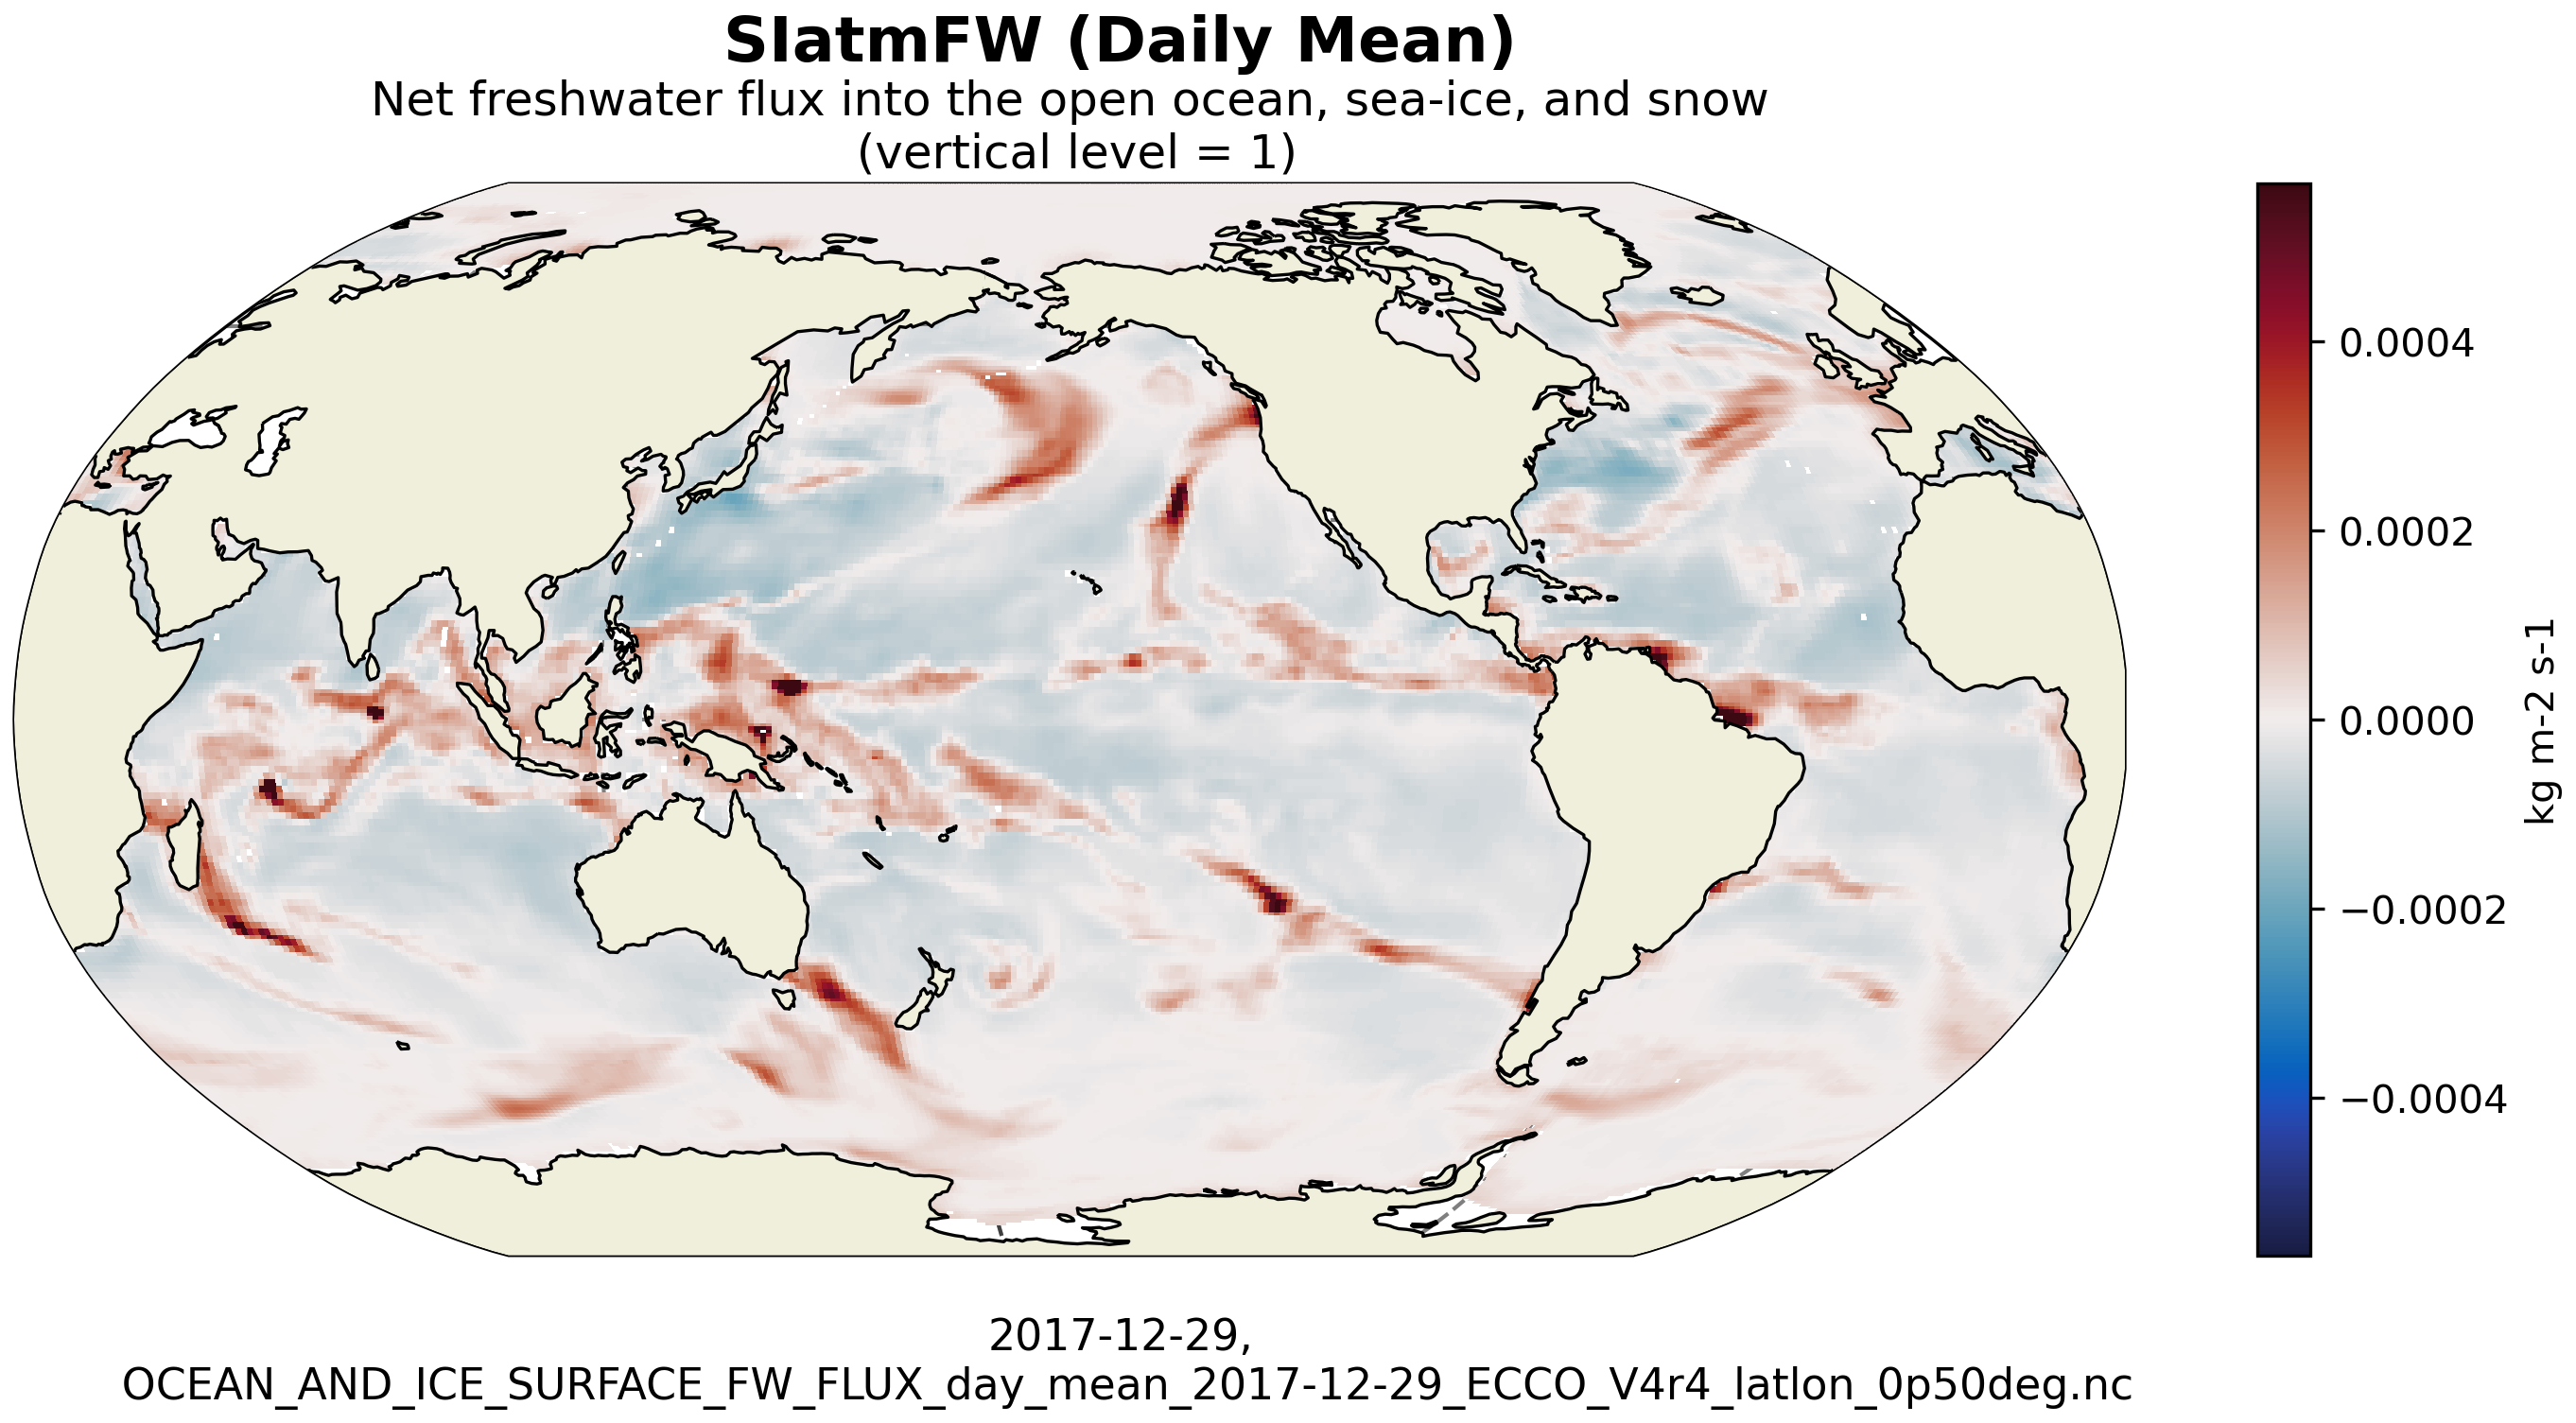
\includegraphics[scale=0.55]{../images/plots/v4r4/latlon_plots/Ocean_and_Sea-Ice_Surface_Freshwater_Fluxes/SIatmFW.png}
\caption{Dataset: OCEAN\_AND\_ICE\_SURFACE\_FW\_FLUX, Variable: SIatmFW}
\label{tab:table-OCEAN_AND_ICE_SURFACE_FW_FLUX_SIatmFW-Plot}
\end{figure}
\newpage
\pagebreak
\subsubsection{Latlon Variable: SIfwThru}
\begin{longtable}{|m{0.06\textwidth}|m{0.3\textwidth}|m{0.45\textwidth}|m{0.12\textwidth}|}
\caption{Attributes description of the variable 'SIfwThru' from OCEAN\_AND\_ICE\_SURFACE\_FW\_FLUX's  dataset.}
\label{tab:table-OCEAN_AND_ICE_SURFACE_FW_FLUX_SIfwThru} \\ 
\hline \endhead \hline \endfoot
\rowcolor{lightgray} \textbf{Storage Type} & \textbf{Variable Name} & \textbf{Description} & \textbf{Unit} \\ \hline
float32 & SIfwThru & Precipitation through sea-ice & kg m-2 s-1 \\ \hline
\multicolumn{4}{|c|}{\cellcolor{lightgray}{\textbf{Description of the variable in Common Data language (CDL)}}} \\ \hline
\multicolumn{4}{|c|}{\fontfamily{lmtt}\selectfont{\makecell{\parbox{.95\textwidth}{\vspace*{0.25cm} \footnotesize{float32 SIfwThru(time, latitude, longitude)\\
\hspace*{0.5cm}SIfwThru: \_FillValue = 9.96921e+36\\
\hspace*{0.5cm}SIfwThru: coordinates = time\\
\hspace*{0.5cm}SIfwThru: coverage\_content\_type = modelResult\\
\hspace*{0.5cm}SIfwThru: direction = >0 increases ocean volume\\
\hspace*{0.5cm}SIfwThru: long\_name = Precipitation through sea-ice\\
\hspace*{0.5cm}SIfwThru: units = kg m-2 s-1\\
\hspace*{0.5cm}SIfwThru: valid\_max = 0.0010632629273459315\\
\hspace*{0.5cm}SIfwThru: valid\_min = -1.695218452368863e-05\\
}}}}} \\ \hline
\rowcolor{lightgray} \multicolumn{4}{|c|}{\textbf{Comments}} \\ \hline
\multicolumn{4}{|p{1\textwidth}|}{\footnotesize{{Precipitation over sea-ice covered regions reaching ocean through sea-ice. note: precipitation over sea-ice covered regions that directly reaches ocean through the sea-ice. it is not due to melt of sea-ice/snow.}}} \\ \hline
\end{longtable}

\begin{figure}[H]
\centering
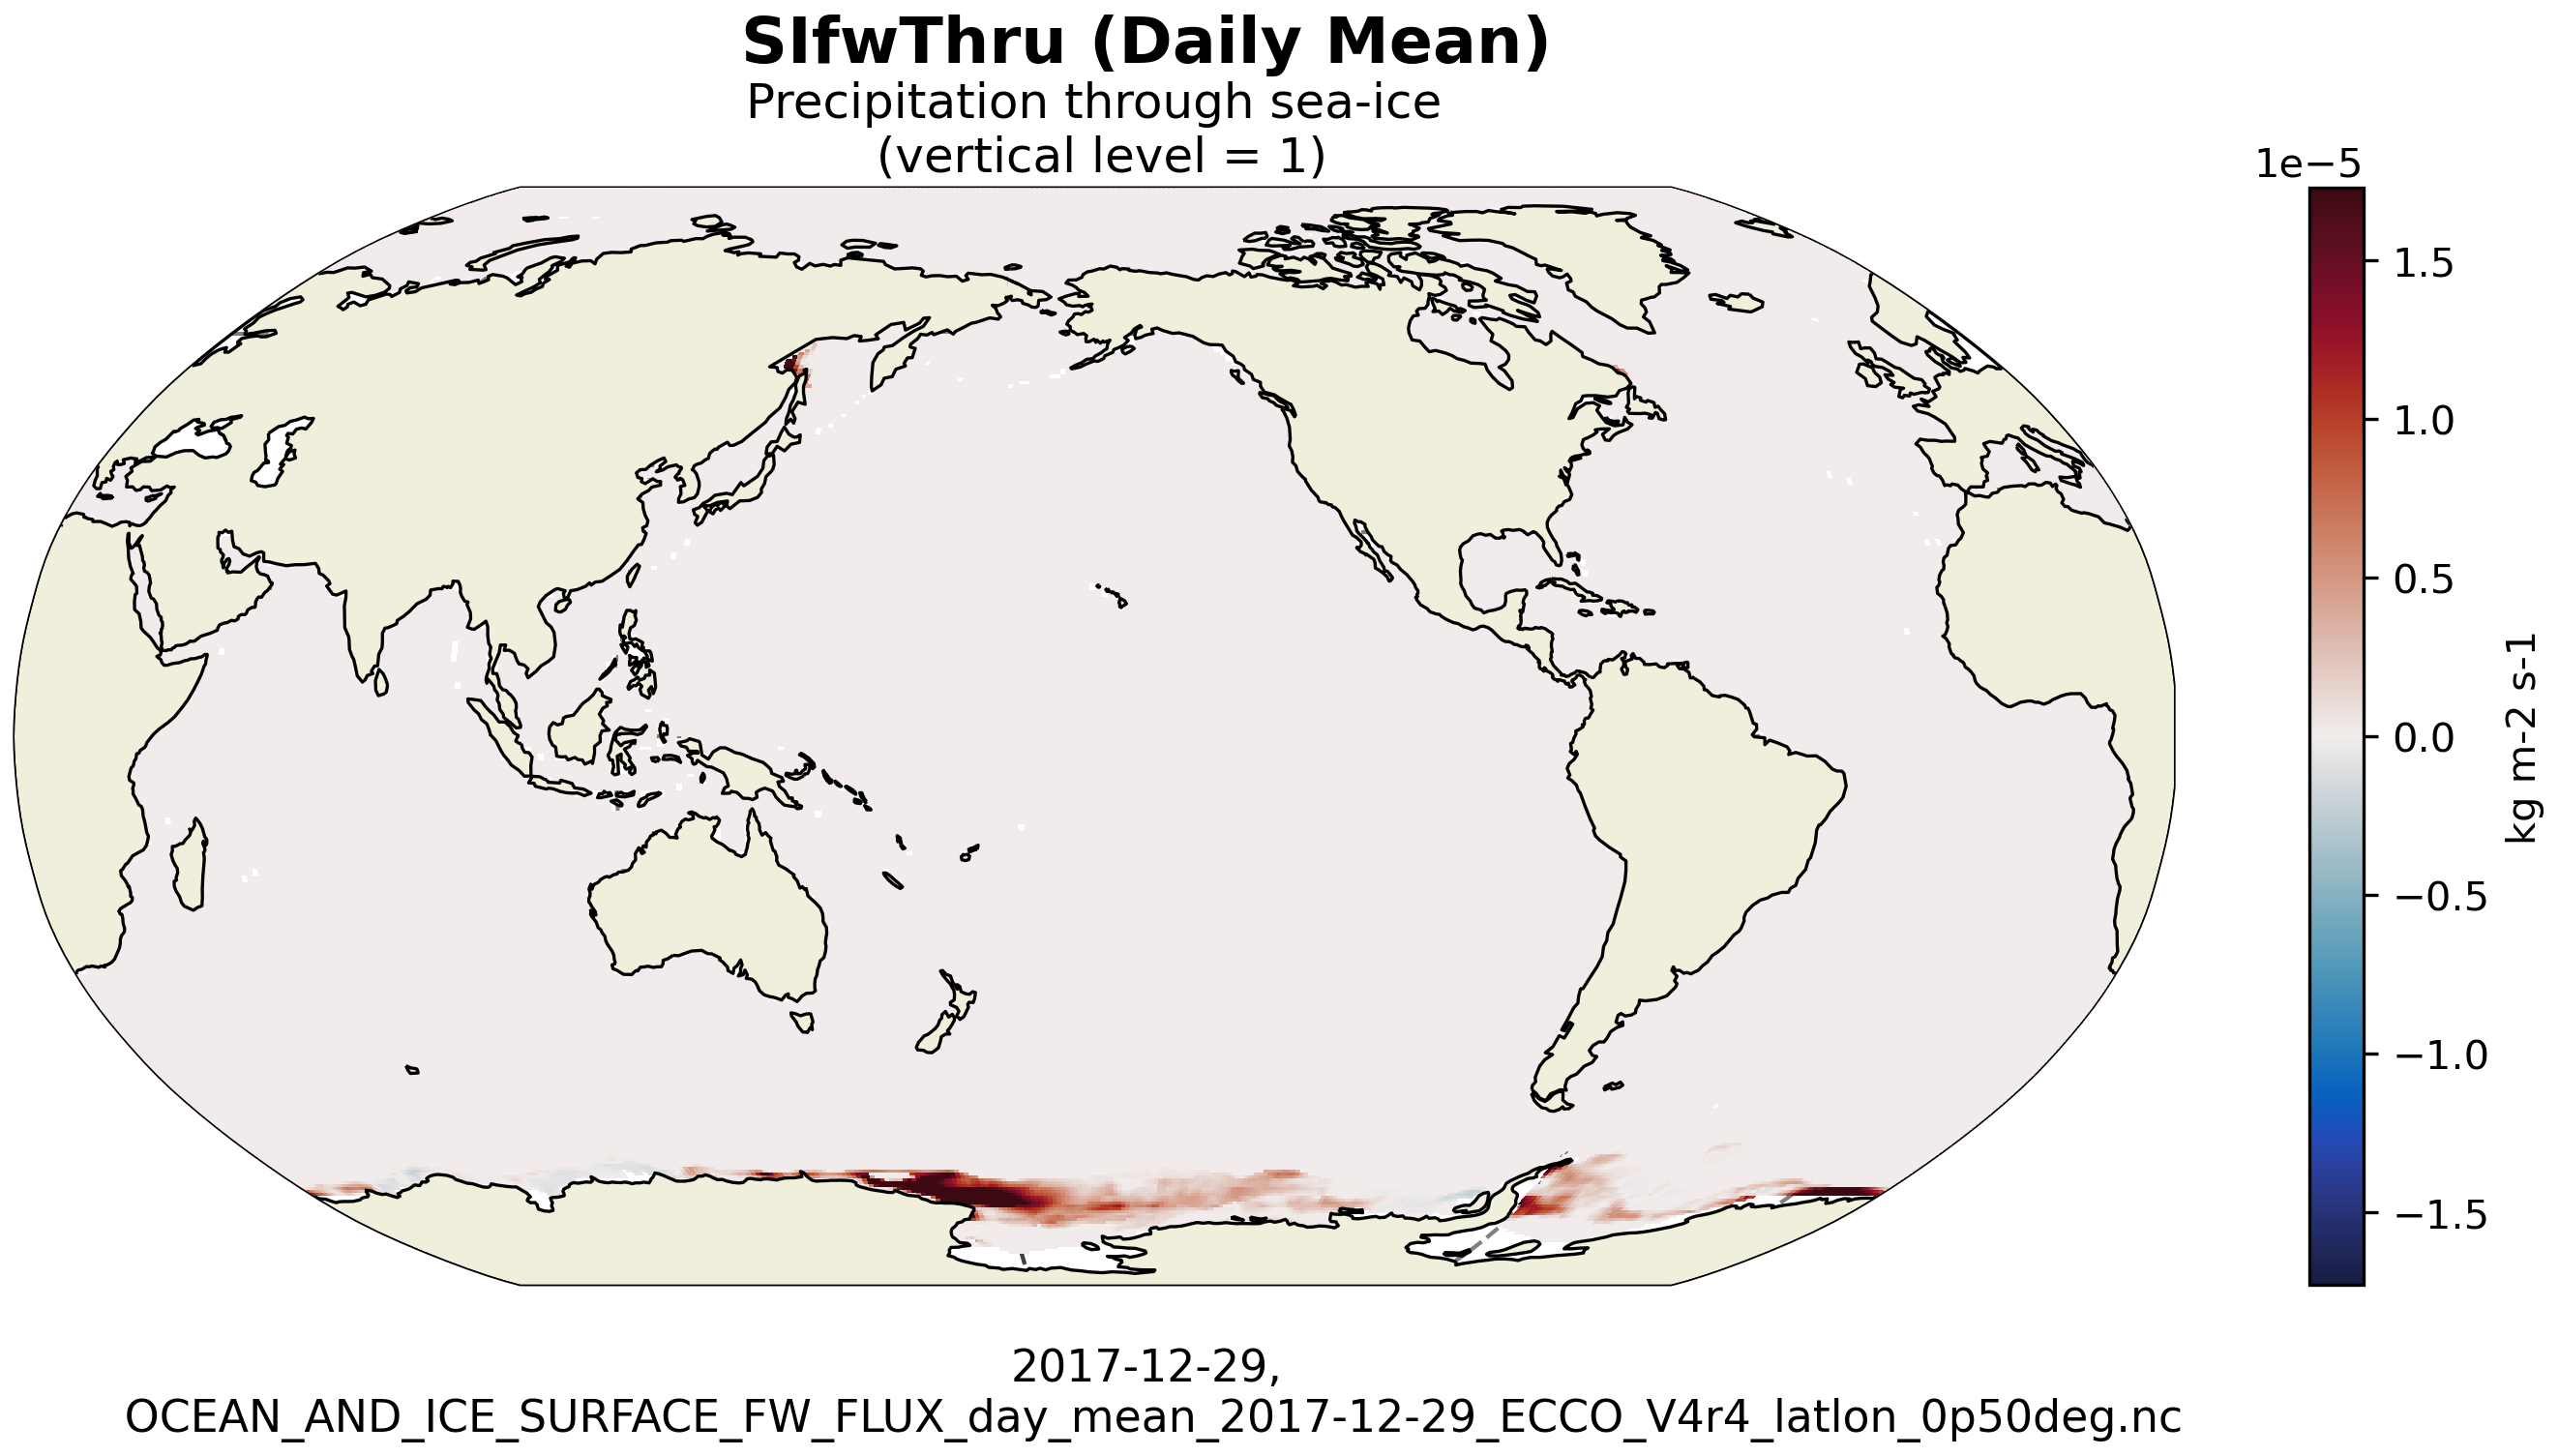
\includegraphics[scale=0.55]{../images/plots/v4r4/latlon_plots/Ocean_and_Sea-Ice_Surface_Freshwater_Fluxes/SIfwThru.png}
\caption{Dataset: OCEAN\_AND\_ICE\_SURFACE\_FW\_FLUX, Variable: SIfwThru}
\label{tab:table-OCEAN_AND_ICE_SURFACE_FW_FLUX_SIfwThru-Plot}
\end{figure}
\newpage
\pagebreak
\subsubsection{Latlon Variable: SIrsSubl}
\begin{longtable}{|m{0.06\textwidth}|m{0.3\textwidth}|m{0.45\textwidth}|m{0.12\textwidth}|}
\caption{Attributes description of the variable 'SIrsSubl' from OCEAN\_AND\_ICE\_SURFACE\_FW\_FLUX's  dataset.}
\label{tab:table-OCEAN_AND_ICE_SURFACE_FW_FLUX_SIrsSubl} \\ 
\hline \endhead \hline \endfoot
\rowcolor{lightgray} \textbf{Storage Type} & \textbf{Variable Name} & \textbf{Description} & \textbf{Unit} \\ \hline
float32 & SIrsSubl & Residual sublimation freshwater flux & kg m-2 s-1 \\ \hline
\multicolumn{4}{|c|}{\cellcolor{lightgray}{\textbf{Description of the variable in Common Data language (CDL)}}} \\ \hline
\multicolumn{4}{|c|}{\fontfamily{lmtt}\selectfont{\makecell{\parbox{.95\textwidth}{\vspace*{0.25cm} \footnotesize{float32 SIrsSubl(time, latitude, longitude)\\
\hspace*{0.5cm}SIrsSubl: \_FillValue = 9.96921e+36\\
\hspace*{0.5cm}SIrsSubl: coordinates = time\\
\hspace*{0.5cm}SIrsSubl: coverage\_content\_type = modelResult\\
\hspace*{0.5cm}SIrsSubl: direction = >0 decreases ocean volume\\
\hspace*{0.5cm}SIrsSubl: long\_name = Residual sublimation freshwater flux\\
\hspace*{0.5cm}SIrsSubl: units = kg m-2 s-1\\
\hspace*{0.5cm}SIrsSubl: valid\_max = 8.640533451398369e-06\\
\hspace*{0.5cm}SIrsSubl: valid\_min = -0.0001067528864950873\\
}}}}} \\ \hline
\rowcolor{lightgray} \multicolumn{4}{|c|}{\textbf{Comments}} \\ \hline
\multicolumn{4}{|p{1\textwidth}|}{\footnotesize{{Residual freshwater flux by sublimation to remove water from or add water to ocean. when implied sublimation freshwater flux siacsubl is larger than availabe sea-ice/snow, sirssubl is positive and water is removed from ocean. note: freshwater flux by sublimation that is to remove water from the ocean when it is positive.}}} \\ \hline
\end{longtable}

\begin{figure}[H]
\centering
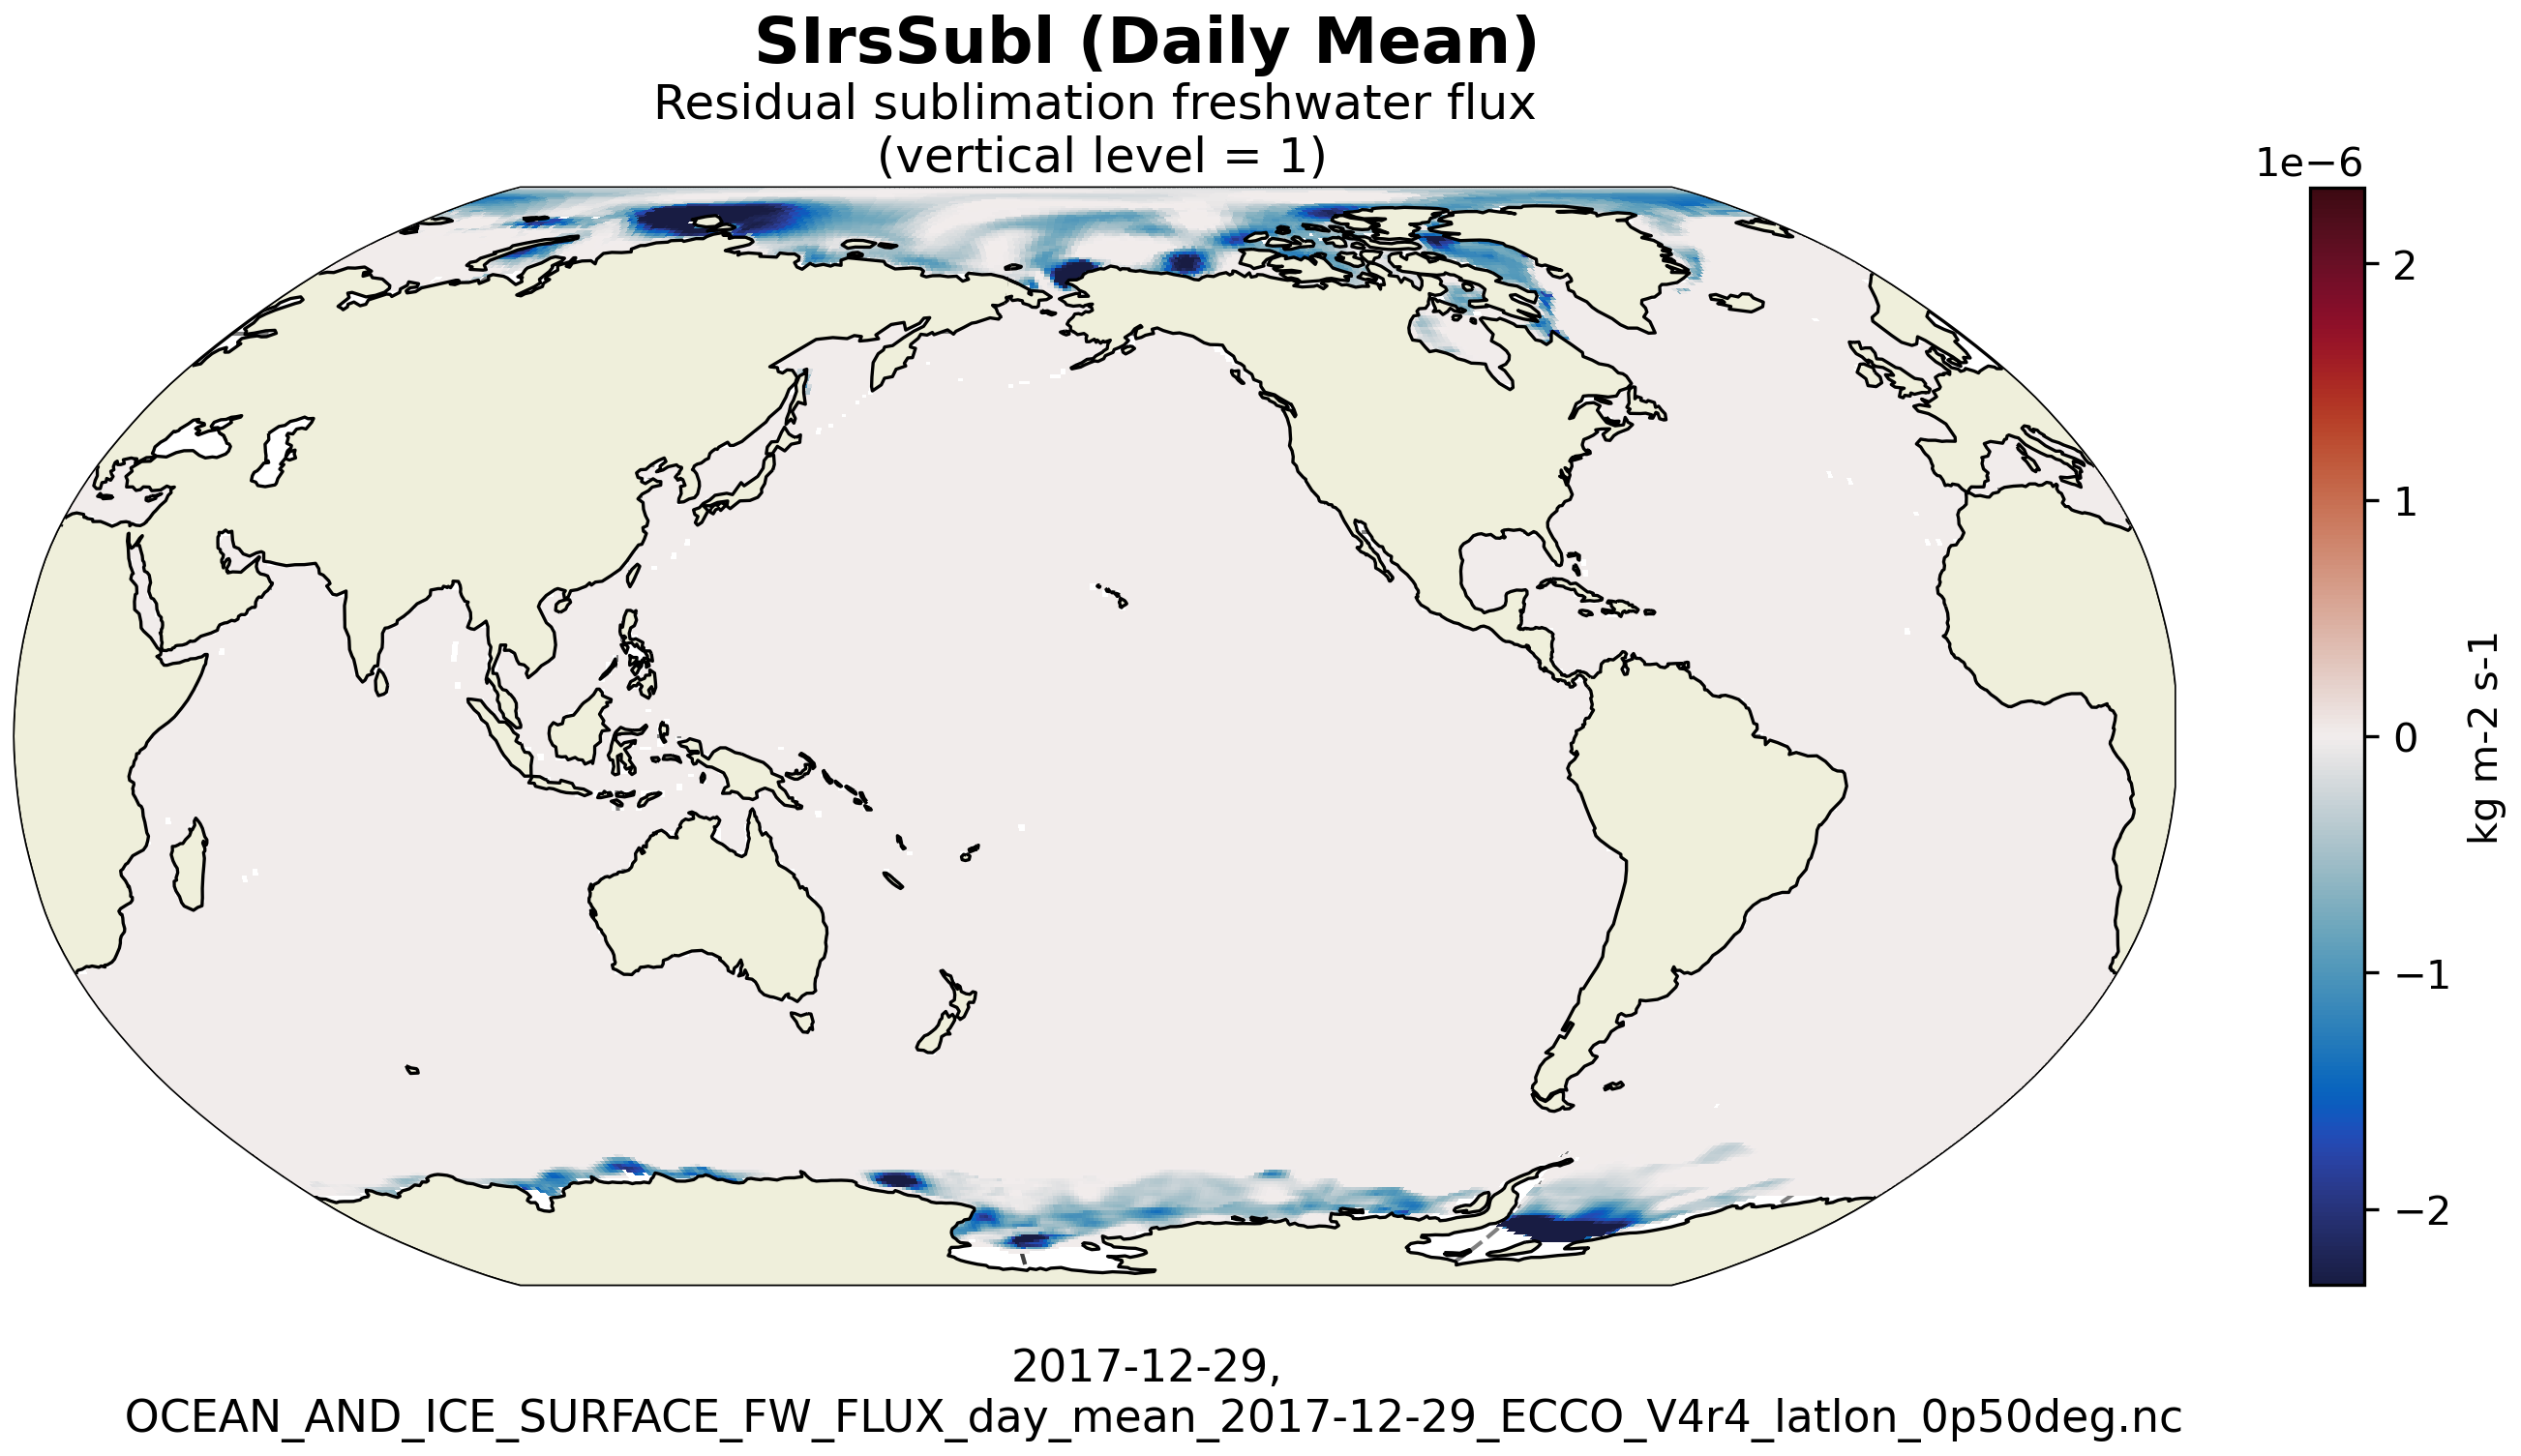
\includegraphics[scale=0.55]{../images/plots/v4r4/latlon_plots/Ocean_and_Sea-Ice_Surface_Freshwater_Fluxes/SIrsSubl.png}
\caption{Dataset: OCEAN\_AND\_ICE\_SURFACE\_FW\_FLUX, Variable: SIrsSubl}
\label{tab:table-OCEAN_AND_ICE_SURFACE_FW_FLUX_SIrsSubl-Plot}
\end{figure}
\newpage
\pagebreak
\subsubsection{Latlon Variable: SIsnPrcp}
\begin{longtable}{|m{0.06\textwidth}|m{0.3\textwidth}|m{0.45\textwidth}|m{0.12\textwidth}|}
\caption{Attributes description of the variable 'SIsnPrcp' from OCEAN\_AND\_ICE\_SURFACE\_FW\_FLUX's  dataset.}
\label{tab:table-OCEAN_AND_ICE_SURFACE_FW_FLUX_SIsnPrcp} \\ 
\hline \endhead \hline \endfoot
\rowcolor{lightgray} \textbf{Storage Type} & \textbf{Variable Name} & \textbf{Description} & \textbf{Unit} \\ \hline
float32 & SIsnPrcp & Snow precipitation on sea-ice & kg m-2 s-1 \\ \hline
\multicolumn{4}{|c|}{\cellcolor{lightgray}{\textbf{Description of the variable in Common Data language (CDL)}}} \\ \hline
\multicolumn{4}{|c|}{\fontfamily{lmtt}\selectfont{\makecell{\parbox{.95\textwidth}{\vspace*{0.25cm} \footnotesize{float32 SIsnPrcp(time, latitude, longitude)\\
\hspace*{0.5cm}SIsnPrcp: \_FillValue = 9.96921e+36\\
\hspace*{0.5cm}SIsnPrcp: coordinates = time\\
\hspace*{0.5cm}SIsnPrcp: coverage\_content\_type = modelResult\\
\hspace*{0.5cm}SIsnPrcp: direction = >0 increases snow thickness (HSNOW)\\
\hspace*{0.5cm}SIsnPrcp: long\_name = Snow precipitation on sea-ice\\
\hspace*{0.5cm}SIsnPrcp: standard\_name = snowfall flux\\
\hspace*{0.5cm}SIsnPrcp: units = kg m-2 s-1\\
\hspace*{0.5cm}SIsnPrcp: valid\_max = 0.0009354020585305989\\
\hspace*{0.5cm}SIsnPrcp: valid\_min = -4.334669574745931e-05\\
}}}}} \\ \hline
\rowcolor{lightgray} \multicolumn{4}{|c|}{\textbf{Comments}} \\ \hline
\multicolumn{4}{|p{1\textwidth}|}{\footnotesize{{Snow precipitation rate over sea-ice, averaged over the entire model grid cell.}}} \\ \hline
\end{longtable}

\begin{figure}[H]
\centering
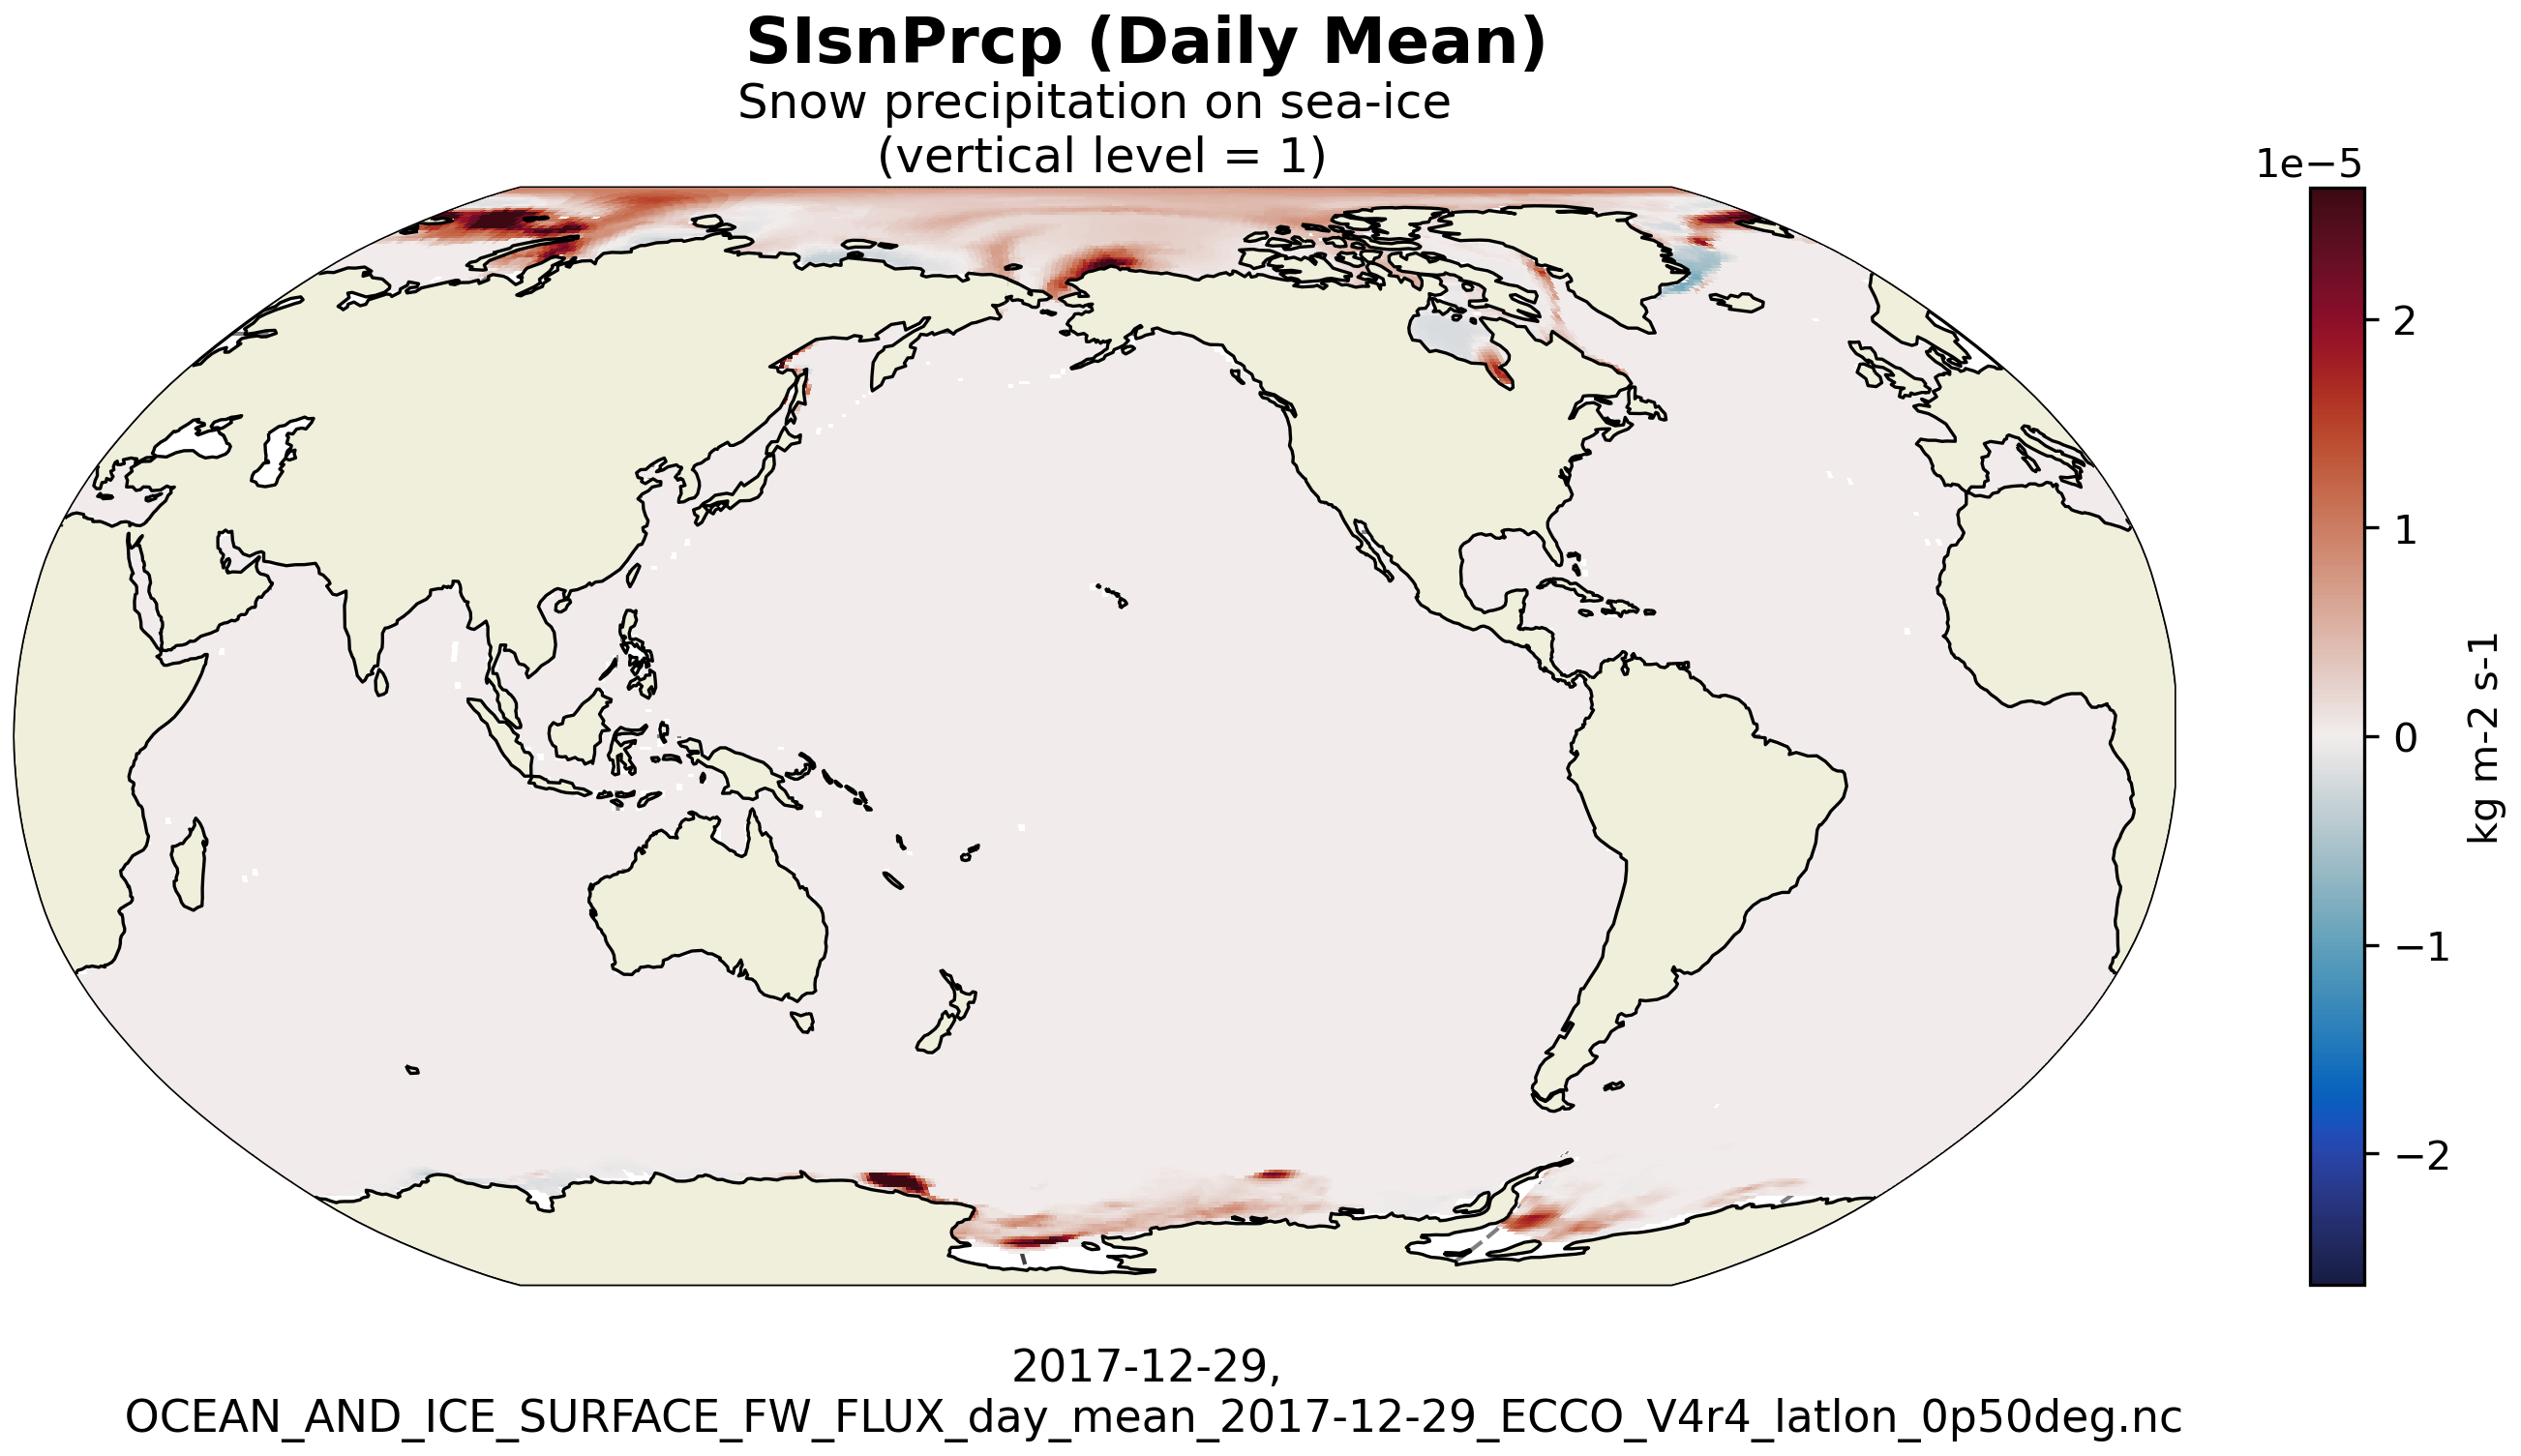
\includegraphics[scale=0.55]{../images/plots/v4r4/latlon_plots/Ocean_and_Sea-Ice_Surface_Freshwater_Fluxes/SIsnPrcp.png}
\caption{Dataset: OCEAN\_AND\_ICE\_SURFACE\_FW\_FLUX, Variable: SIsnPrcp}
\label{tab:table-OCEAN_AND_ICE_SURFACE_FW_FLUX_SIsnPrcp-Plot}
\end{figure}
\newpage
\pagebreak
\subsubsection{Latlon Variable: oceFWflx}
\begin{longtable}{|m{0.06\textwidth}|m{0.3\textwidth}|m{0.45\textwidth}|m{0.12\textwidth}|}
\caption{Attributes description of the variable 'oceFWflx' from OCEAN\_AND\_ICE\_SURFACE\_FW\_FLUX's  dataset.}
\label{tab:table-OCEAN_AND_ICE_SURFACE_FW_FLUX_oceFWflx} \\ 
\hline \endhead \hline \endfoot
\rowcolor{lightgray} \textbf{Storage Type} & \textbf{Variable Name} & \textbf{Description} & \textbf{Unit} \\ \hline
float32 & oceFWflx & Net freshwater flux into the ocean & kg m-2 s-1 \\ \hline
\multicolumn{4}{|c|}{\cellcolor{lightgray}{\textbf{Description of the variable in Common Data language (CDL)}}} \\ \hline
\multicolumn{4}{|c|}{\fontfamily{lmtt}\selectfont{\makecell{\parbox{.95\textwidth}{\vspace*{0.25cm} \footnotesize{float32 oceFWflx(time, latitude, longitude)\\
\hspace*{0.5cm}oceFWflx: \_FillValue = 9.96921e+36\\
\hspace*{0.5cm}oceFWflx: coordinates = time\\
\hspace*{0.5cm}oceFWflx: coverage\_content\_type = modelResult\\
\hspace*{0.5cm}oceFWflx: direction = >0 decreases salinity (SALT)\\
\hspace*{0.5cm}oceFWflx: long\_name = Net freshwater flux into the ocean\\
\hspace*{0.5cm}oceFWflx: standard\_name = water flux into sea water\\
\hspace*{0.5cm}oceFWflx: units = kg m-2 s-1\\
\hspace*{0.5cm}oceFWflx: valid\_max = 0.008299433626234531\\
\hspace*{0.5cm}oceFWflx: valid\_min = -0.0033125500194728374\\
}}}}} \\ \hline
\rowcolor{lightgray} \multicolumn{4}{|c|}{\textbf{Comments}} \\ \hline
\multicolumn{4}{|p{1\textwidth}|}{\footnotesize{{Net freshwater flux into the ocean including contributions from runoff, evaporation, precipitation, and mass exchange with sea-ice due to melting and freezing and snow melting. note: ocefwflx does not include freshwater fluxes between the atmosphere and sea-ice and snow. the variable 'siatmfw' accounts for freshwater fluxes out of the combined ocean+sea-ice+snow reservoir.}}} \\ \hline
\end{longtable}

\begin{figure}[H]
\centering
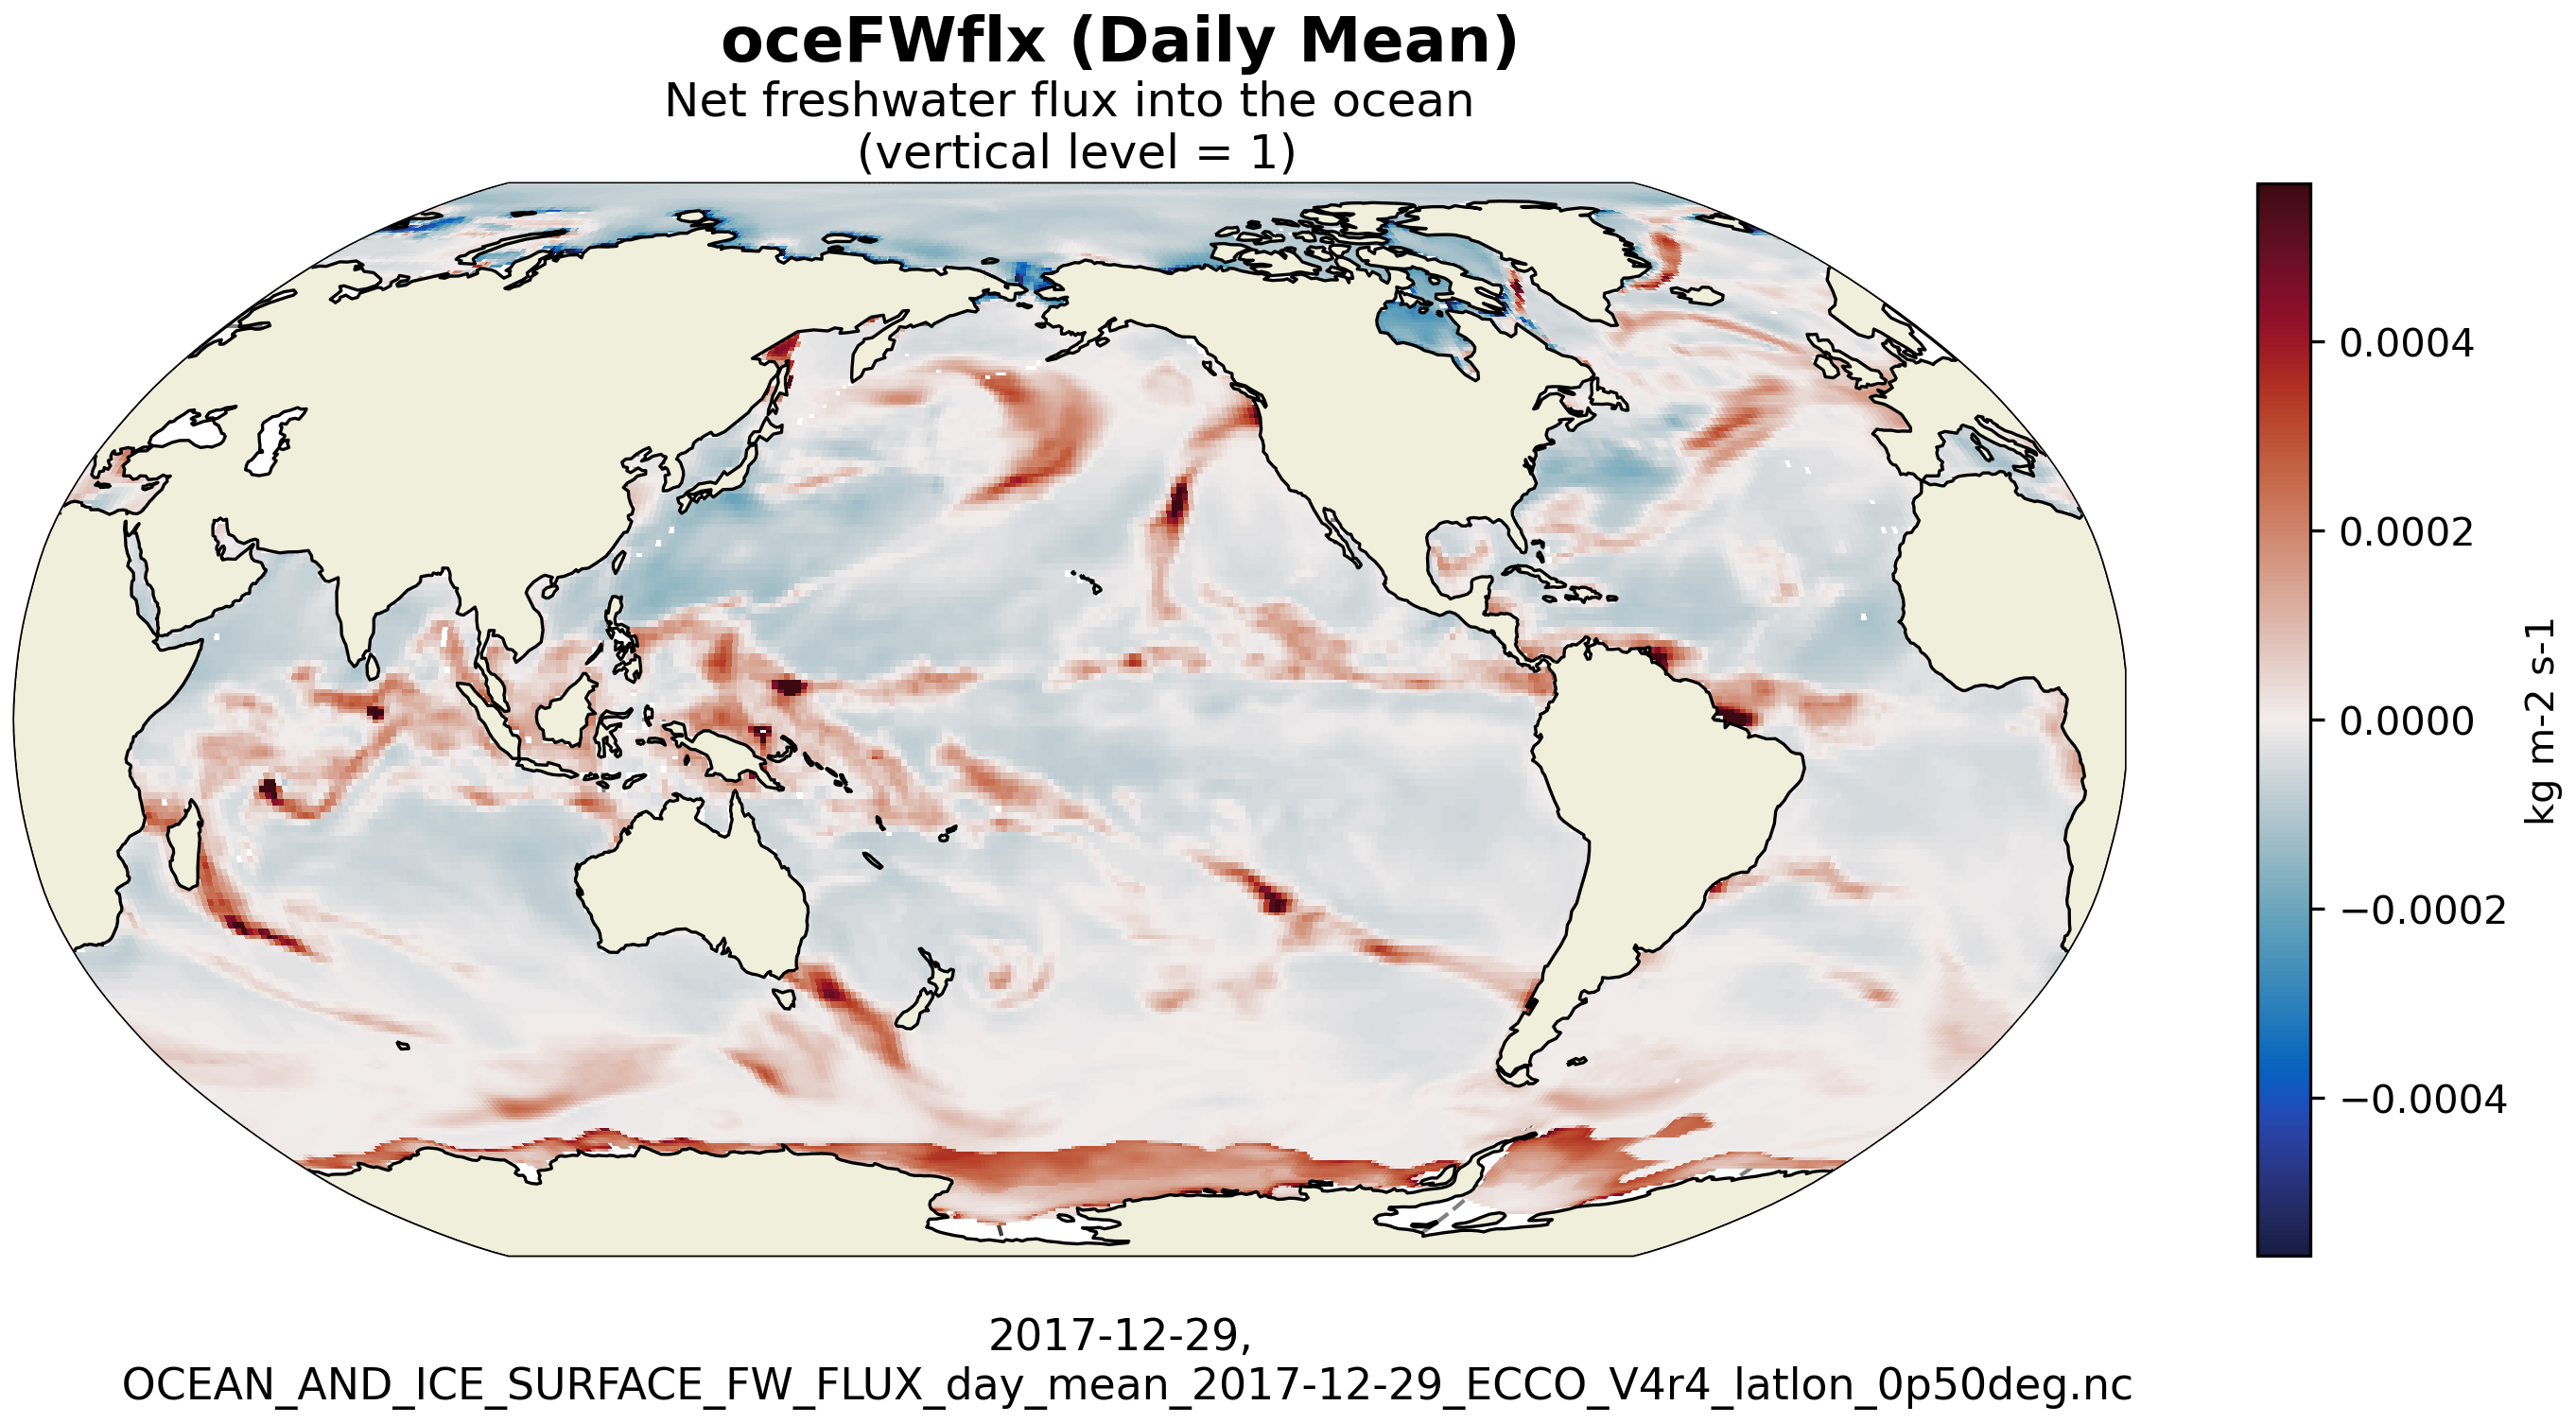
\includegraphics[scale=0.55]{../images/plots/v4r4/latlon_plots/Ocean_and_Sea-Ice_Surface_Freshwater_Fluxes/oceFWflx.png}
\caption{Dataset: OCEAN\_AND\_ICE\_SURFACE\_FW\_FLUX, Variable: oceFWflx}
\label{tab:table-OCEAN_AND_ICE_SURFACE_FW_FLUX_oceFWflx-Plot}
\end{figure}
\newpage
\subsection{Latlon dataset of OCEAN\_AND\_ICE\_SURFACE\_HEAT\_FLUX}
\newp
\subsubsection{Overview}
This dataset provides 2D fields of ocean and sea-ice surface heat fluxes interpolated to a regular 0.5-degree grid from the ECCO Version 4 Release 4 (V4r4) ocean and sea-ice state estimate. The dataset is provided on daily-average and monthly-average time resolution. 
\begin{longtable}{|m{0.15\textwidth}|m{0.64\textwidth}|m{0.12\textwidth}|}
\caption{Coordinates and Variables in the dataset OCEAN\_AND\_ICE\_SURFACE\_HEAT\_FLUX}
\label{tab:table-OCEAN_AND_ICE_SURFACE_HEAT_FLUX-fields} \\ 
\hline \endhead \hline \endfoot
\rowcolor{lightgray} \multicolumn{1}{|c|}{\textbf{Coordinates}} & \multicolumn{1}{|c|}{\textbf{Description of data coordinates}} &  \multicolumn{1}{|c|}{\textbf{Unit}}\\ \hline
time &Center time of averaging period &--none--  \\ \hline
latitude &Latitude at grid cell center &degrees\_north  \\ \hline
longitude &Longitude at grid cell center &degrees\_east  \\ \hline
time\_bnds &Time bounds of averaging period &--none--  \\ \hline
latitude\_bnds &Latitude bounds grid cells &--none--  \\ \hline
longitude\_bnds &Longitude bounds grid cells &--none--  \\ \hline
\rowcolor{lightgray} \multicolumn{1}{|c|}{\textbf{Variables}} & \multicolumn{1}{|c|}{\textbf{Description of data variables}} &  \multicolumn{1}{|c|}{\textbf{Unit}}\\ \hline
EXFhl &Open ocean air-sea latent heat flux &W m-2  \\ \hline
EXFhs &Open ocean air-sea sensible heat flux &W m-2  \\ \hline
EXFlwdn &Downward longwave radiative flux &W m-2  \\ \hline
EXFswdn &Downwelling shortwave radiative flux &W m-2  \\ \hline
EXFqnet &Open ocean net air-sea heat flux &W m-2  \\ \hline
oceQnet &Net heat flux into the ocean surface &W m-2  \\ \hline
SIatmQnt &Net upward heat flux to the atmosphere &W m-2  \\ \hline
TFLUX &Rate of change of ocean heat content per m2 accounting for mass fluxes. &W m-2  \\ \hline
EXFswnet &Open ocean net shortwave radiative flux &W m-2  \\ \hline
EXFlwnet &Net open ocean longwave radiative flux &W m-2  \\ \hline
oceQsw &Net shortwave radiative flux across the ocean surface &W m-2  \\ \hline
SIaaflux &Conservative ocean and sea-ice advective heat flux adjustment &W m-2  \\ \hline
\end{longtable}

\newp
\pagebreak
\subsubsection{Latlon Variable: EXFhl}
\begin{longtable}{|m{0.06\textwidth}|m{0.3\textwidth}|m{0.45\textwidth}|m{0.12\textwidth}|}
\caption{Attributes description of the variable 'EXFhl' from OCEAN\_AND\_ICE\_SURFACE\_HEAT\_FLUX's  dataset.}
\label{tab:table-OCEAN_AND_ICE_SURFACE_HEAT_FLUX_EXFhl} \\ 
\hline \endhead \hline \endfoot
\rowcolor{lightgray} \textbf{Storage Type} & \textbf{Variable Name} & \textbf{Description} & \textbf{Unit} \\ \hline
float32 & EXFhl & Open ocean air-sea latent heat flux & W m-2 \\ \hline
\multicolumn{4}{|c|}{\cellcolor{lightgray}{\textbf{Description of the variable in Common Data language (CDL)}}} \\ \hline
\multicolumn{4}{|c|}{\fontfamily{lmtt}\selectfont{\makecell{\parbox{.95\textwidth}{\vspace*{0.25cm} \footnotesize{float32 EXFhl(time, latitude, longitude)\\
\hspace*{0.5cm}EXFhl: \_FillValue = 9.96921e+36\\
\hspace*{0.5cm}EXFhl: coordinates = time\\
\hspace*{0.5cm}EXFhl: coverage\_content\_type = modelResult\\
\hspace*{0.5cm}EXFhl: direction = >0 increases potential temperature (THETA)\\
\hspace*{0.5cm}EXFhl: long\_name = Open ocean air-sea latent heat flux\\
\hspace*{0.5cm}EXFhl: standard\_name = surface downward latent heat flux\\
\hspace*{0.5cm}EXFhl: units = W m-2\\
\hspace*{0.5cm}EXFhl: valid\_max = 273.9528503417969\\
\hspace*{0.5cm}EXFhl: valid\_min = -1772.513671875\\
}}}}} \\ \hline
\rowcolor{lightgray} \multicolumn{4}{|c|}{\textbf{Comments}} \\ \hline
\multicolumn{4}{|p{1\textwidth}|}{\footnotesize{{Air-sea latent heat flux per unit area of open water (not covered by sea-ice). note: calculated from the bulk formula following large and yeager (2004) ncar/tn-460+str.}}} \\ \hline
\end{longtable}

\begin{figure}[H]
\centering
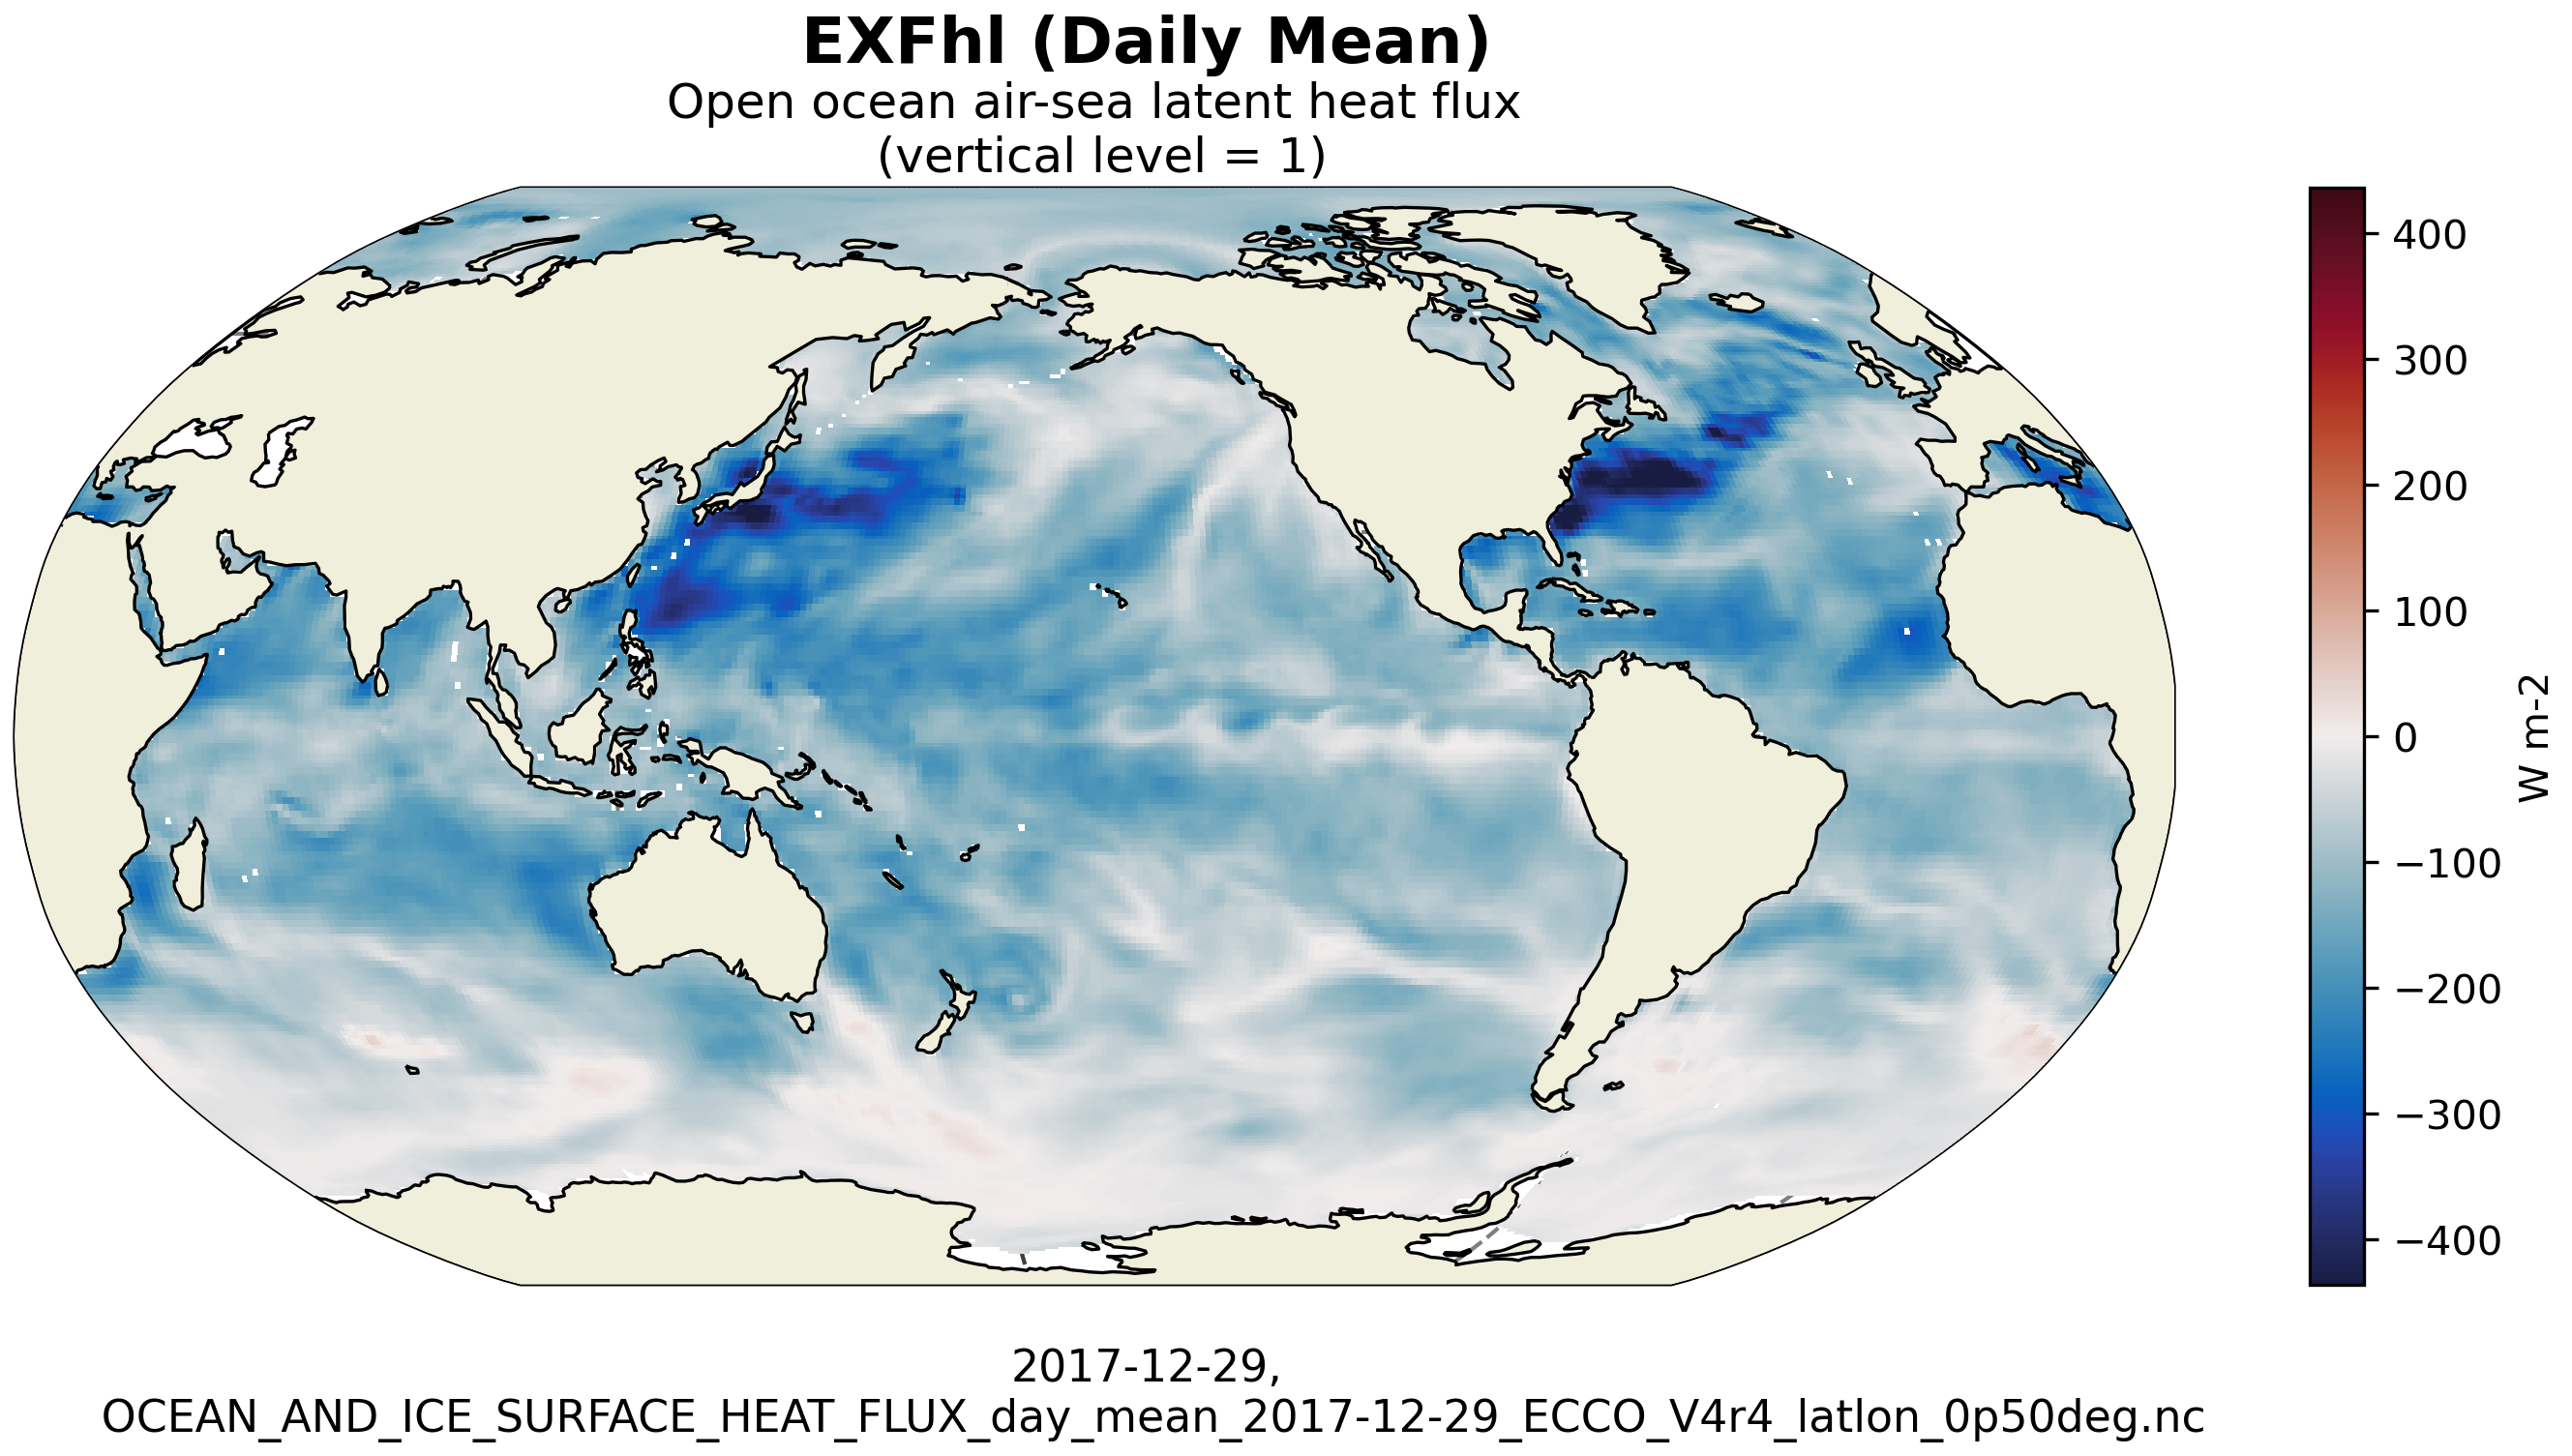
\includegraphics[scale=0.55]{../images/plots/v4r4/latlon_plots/Ocean_and_Sea-Ice_Surface_Heat_Fluxes/EXFhl.png}
\caption{Dataset: OCEAN\_AND\_ICE\_SURFACE\_HEAT\_FLUX, Variable: EXFhl}
\label{tab:table-OCEAN_AND_ICE_SURFACE_HEAT_FLUX_EXFhl-Plot}
\end{figure}
\newpage
\pagebreak
\subsubsection{Latlon Variable: EXFhs}
\begin{longtable}{|m{0.06\textwidth}|m{0.3\textwidth}|m{0.45\textwidth}|m{0.12\textwidth}|}
\caption{Attributes description of the variable 'EXFhs' from OCEAN\_AND\_ICE\_SURFACE\_HEAT\_FLUX's  dataset.}
\label{tab:table-OCEAN_AND_ICE_SURFACE_HEAT_FLUX_EXFhs} \\ 
\hline \endhead \hline \endfoot
\rowcolor{lightgray} \textbf{Storage Type} & \textbf{Variable Name} & \textbf{Description} & \textbf{Unit} \\ \hline
float32 & EXFhs & Open ocean air-sea sensible heat flux & W m-2 \\ \hline
\multicolumn{4}{|c|}{\cellcolor{lightgray}{\textbf{Description of the variable in Common Data language (CDL)}}} \\ \hline
\multicolumn{4}{|c|}{\fontfamily{lmtt}\selectfont{\makecell{\parbox{.95\textwidth}{\vspace*{0.25cm} \footnotesize{float32 EXFhs(time, latitude, longitude)\\
\hspace*{0.5cm}EXFhs: \_FillValue = 9.96921e+36\\
\hspace*{0.5cm}EXFhs: coordinates = time\\
\hspace*{0.5cm}EXFhs: coverage\_content\_type = modelResult\\
\hspace*{0.5cm}EXFhs: direction = >0 increases potential temperature (THETA)\\
\hspace*{0.5cm}EXFhs: long\_name = Open ocean air-sea sensible heat flux\\
\hspace*{0.5cm}EXFhs: standard\_name = surface downward sensible heat flux\\
\hspace*{0.5cm}EXFhs: units = W m-2\\
\hspace*{0.5cm}EXFhs: valid\_max = 357.0105895996094\\
\hspace*{0.5cm}EXFhs: valid\_min = -2478.766357421875\\
}}}}} \\ \hline
\rowcolor{lightgray} \multicolumn{4}{|c|}{\textbf{Comments}} \\ \hline
\multicolumn{4}{|p{1\textwidth}|}{\footnotesize{{Air-sea sensible heat flux per unit area of open water (not covered by sea-ice). note: calculated from the bulk formula following large and yeager (2004) ncar/tn-460+str.}}} \\ \hline
\end{longtable}

\begin{figure}[H]
\centering
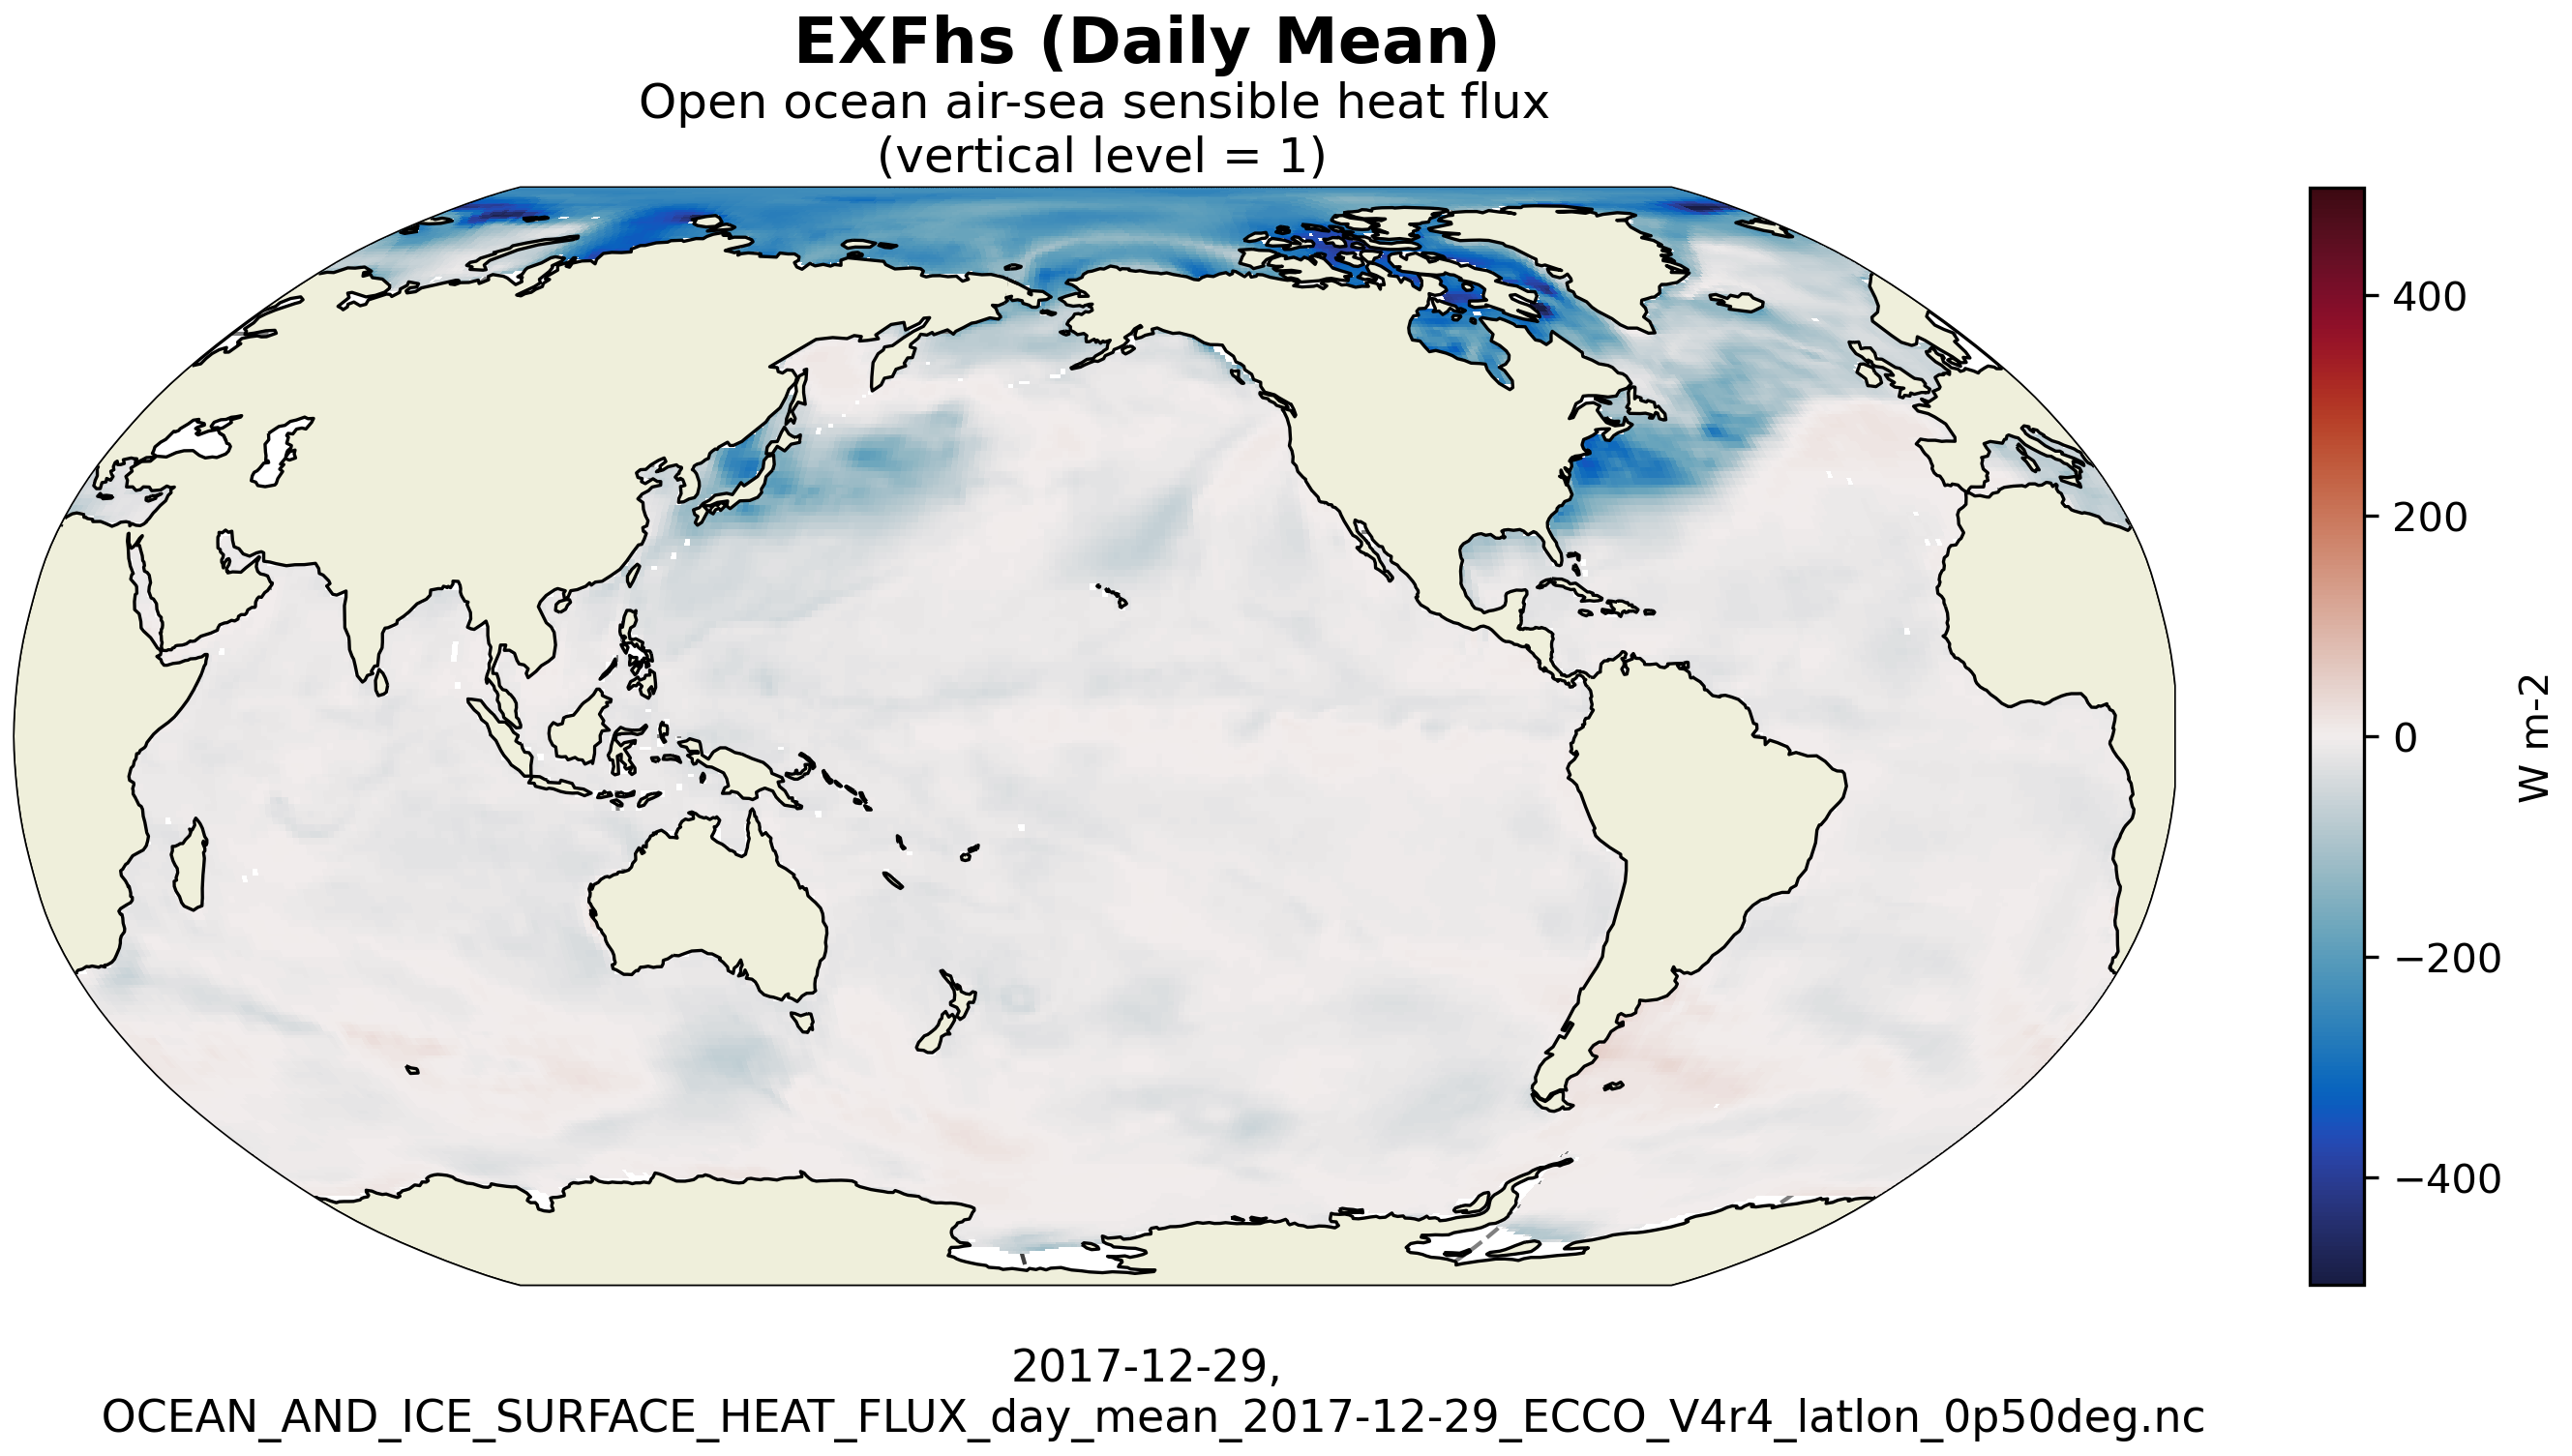
\includegraphics[scale=0.55]{../images/plots/v4r4/latlon_plots/Ocean_and_Sea-Ice_Surface_Heat_Fluxes/EXFhs.png}
\caption{Dataset: OCEAN\_AND\_ICE\_SURFACE\_HEAT\_FLUX, Variable: EXFhs}
\label{tab:table-OCEAN_AND_ICE_SURFACE_HEAT_FLUX_EXFhs-Plot}
\end{figure}
\newpage
\pagebreak
\subsubsection{Latlon Variable: EXFlwdn}
\begin{longtable}{|m{0.06\textwidth}|m{0.3\textwidth}|m{0.45\textwidth}|m{0.12\textwidth}|}
\caption{Attributes description of the variable 'EXFlwdn' from OCEAN\_AND\_ICE\_SURFACE\_HEAT\_FLUX's  dataset.}
\label{tab:table-OCEAN_AND_ICE_SURFACE_HEAT_FLUX_EXFlwdn} \\ 
\hline \endhead \hline \endfoot
\rowcolor{lightgray} \textbf{Storage Type} & \textbf{Variable Name} & \textbf{Description} & \textbf{Unit} \\ \hline
float32 & EXFlwdn & Downward longwave radiative flux & W m-2 \\ \hline
\multicolumn{4}{|c|}{\cellcolor{lightgray}{\textbf{Description of the variable in Common Data language (CDL)}}} \\ \hline
\multicolumn{4}{|c|}{\fontfamily{lmtt}\selectfont{\makecell{\parbox{.95\textwidth}{\vspace*{0.25cm} \footnotesize{float32 EXFlwdn(time, latitude, longitude)\\
\hspace*{0.5cm}EXFlwdn: \_FillValue = 9.96921e+36\\
\hspace*{0.5cm}EXFlwdn: coordinates = time\\
\hspace*{0.5cm}EXFlwdn: coverage\_content\_type = modelResult\\
\hspace*{0.5cm}EXFlwdn: direction = >0 increases potential temperature (THETA)\\
\hspace*{0.5cm}EXFlwdn: long\_name = Downward longwave radiative flux\\
\hspace*{0.5cm}EXFlwdn: standard\_name = surface downwelling longwave flux in air\\
\hspace*{0.5cm}EXFlwdn: units = W m-2\\
\hspace*{0.5cm}EXFlwdn: valid\_max = 513.3919067382812\\
\hspace*{0.5cm}EXFlwdn: valid\_min = 4.188045501708984\\
}}}}} \\ \hline
\rowcolor{lightgray} \multicolumn{4}{|c|}{\textbf{Comments}} \\ \hline
\multicolumn{4}{|p{1\textwidth}|}{\footnotesize{{Downward longwave radiative flux. note: sum of era-interim downward longwave radiation and the control adjustment from ocean state estimation.}}} \\ \hline
\end{longtable}

\begin{figure}[H]
\centering
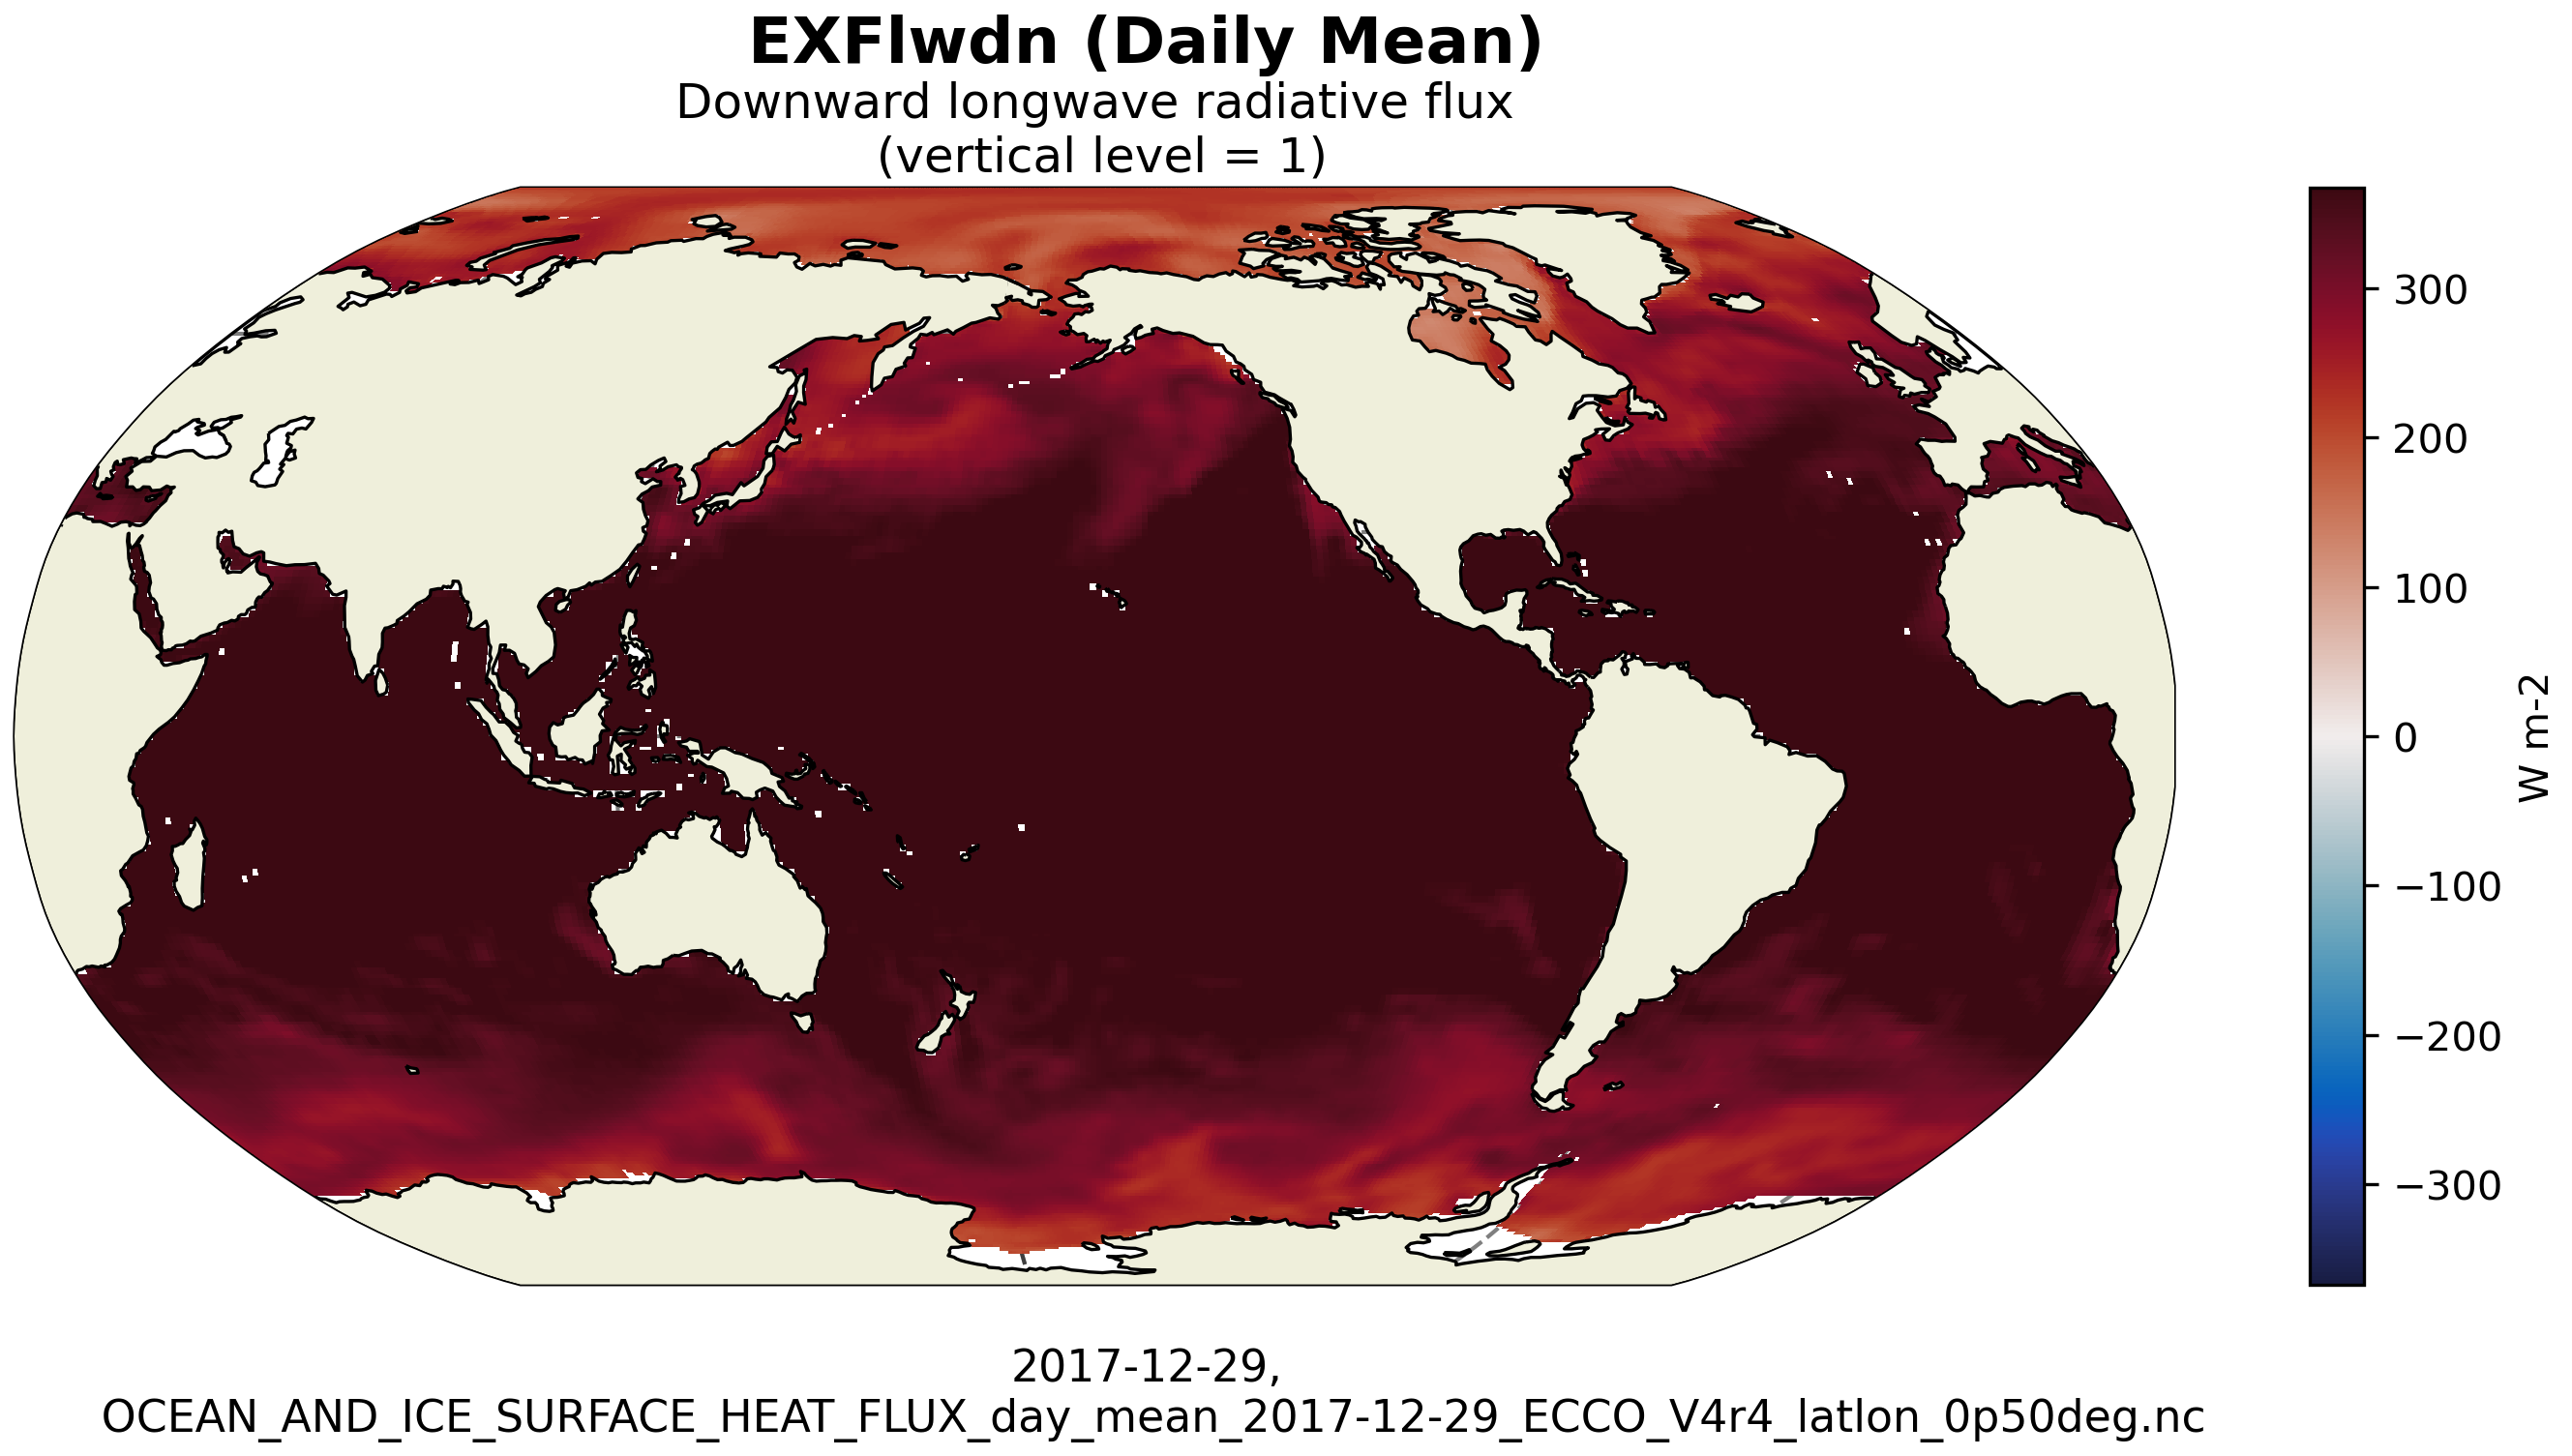
\includegraphics[scale=0.55]{../images/plots/v4r4/latlon_plots/Ocean_and_Sea-Ice_Surface_Heat_Fluxes/EXFlwdn.png}
\caption{Dataset: OCEAN\_AND\_ICE\_SURFACE\_HEAT\_FLUX, Variable: EXFlwdn}
\label{tab:table-OCEAN_AND_ICE_SURFACE_HEAT_FLUX_EXFlwdn-Plot}
\end{figure}
\newpage
\pagebreak
\subsubsection{Latlon Variable: EXFlwnet}
\begin{longtable}{|m{0.06\textwidth}|m{0.3\textwidth}|m{0.45\textwidth}|m{0.12\textwidth}|}
\caption{Attributes description of the variable 'EXFlwnet' from OCEAN\_AND\_ICE\_SURFACE\_HEAT\_FLUX's  dataset.}
\label{tab:table-OCEAN_AND_ICE_SURFACE_HEAT_FLUX_EXFlwnet} \\ 
\hline \endhead \hline \endfoot
\rowcolor{lightgray} \textbf{Storage Type} & \textbf{Variable Name} & \textbf{Description} & \textbf{Unit} \\ \hline
float32 & EXFlwnet & Net open ocean longwave radiative flux & W m-2 \\ \hline
\multicolumn{4}{|c|}{\cellcolor{lightgray}{\textbf{Description of the variable in Common Data language (CDL)}}} \\ \hline
\multicolumn{4}{|c|}{\fontfamily{lmtt}\selectfont{\makecell{\parbox{.95\textwidth}{\vspace*{0.25cm} \footnotesize{float32 EXFlwnet(time, latitude, longitude)\\
\hspace*{0.5cm}EXFlwnet: \_FillValue = 9.96921e+36\\
\hspace*{0.5cm}EXFlwnet: coordinates = time\\
\hspace*{0.5cm}EXFlwnet: coverage\_content\_type = modelResult\\
\hspace*{0.5cm}EXFlwnet: direction = >0 increases potential temperature (THETA)\\
\hspace*{0.5cm}EXFlwnet: long\_name = Net open ocean longwave radiative flux\\
\hspace*{0.5cm}EXFlwnet: standard\_name = surface net downward longwave flux\\
\hspace*{0.5cm}EXFlwnet: units = W m-2\\
\hspace*{0.5cm}EXFlwnet: valid\_max = 293.4114990234375\\
\hspace*{0.5cm}EXFlwnet: valid\_min = -144.3661346435547\\
}}}}} \\ \hline
\rowcolor{lightgray} \multicolumn{4}{|c|}{\textbf{Comments}} \\ \hline
\multicolumn{4}{|p{1\textwidth}|}{\footnotesize{{Net longwave radiative flux per unit area of open water (not covered by sea-ice). note: net longwave radiation over open water calculated from downward longwave radiation (exflwdn) and upward longwave radiation from ocean and sea-ice thermal emission (stefan-boltzman law).}}} \\ \hline
\end{longtable}

\begin{figure}[H]
\centering
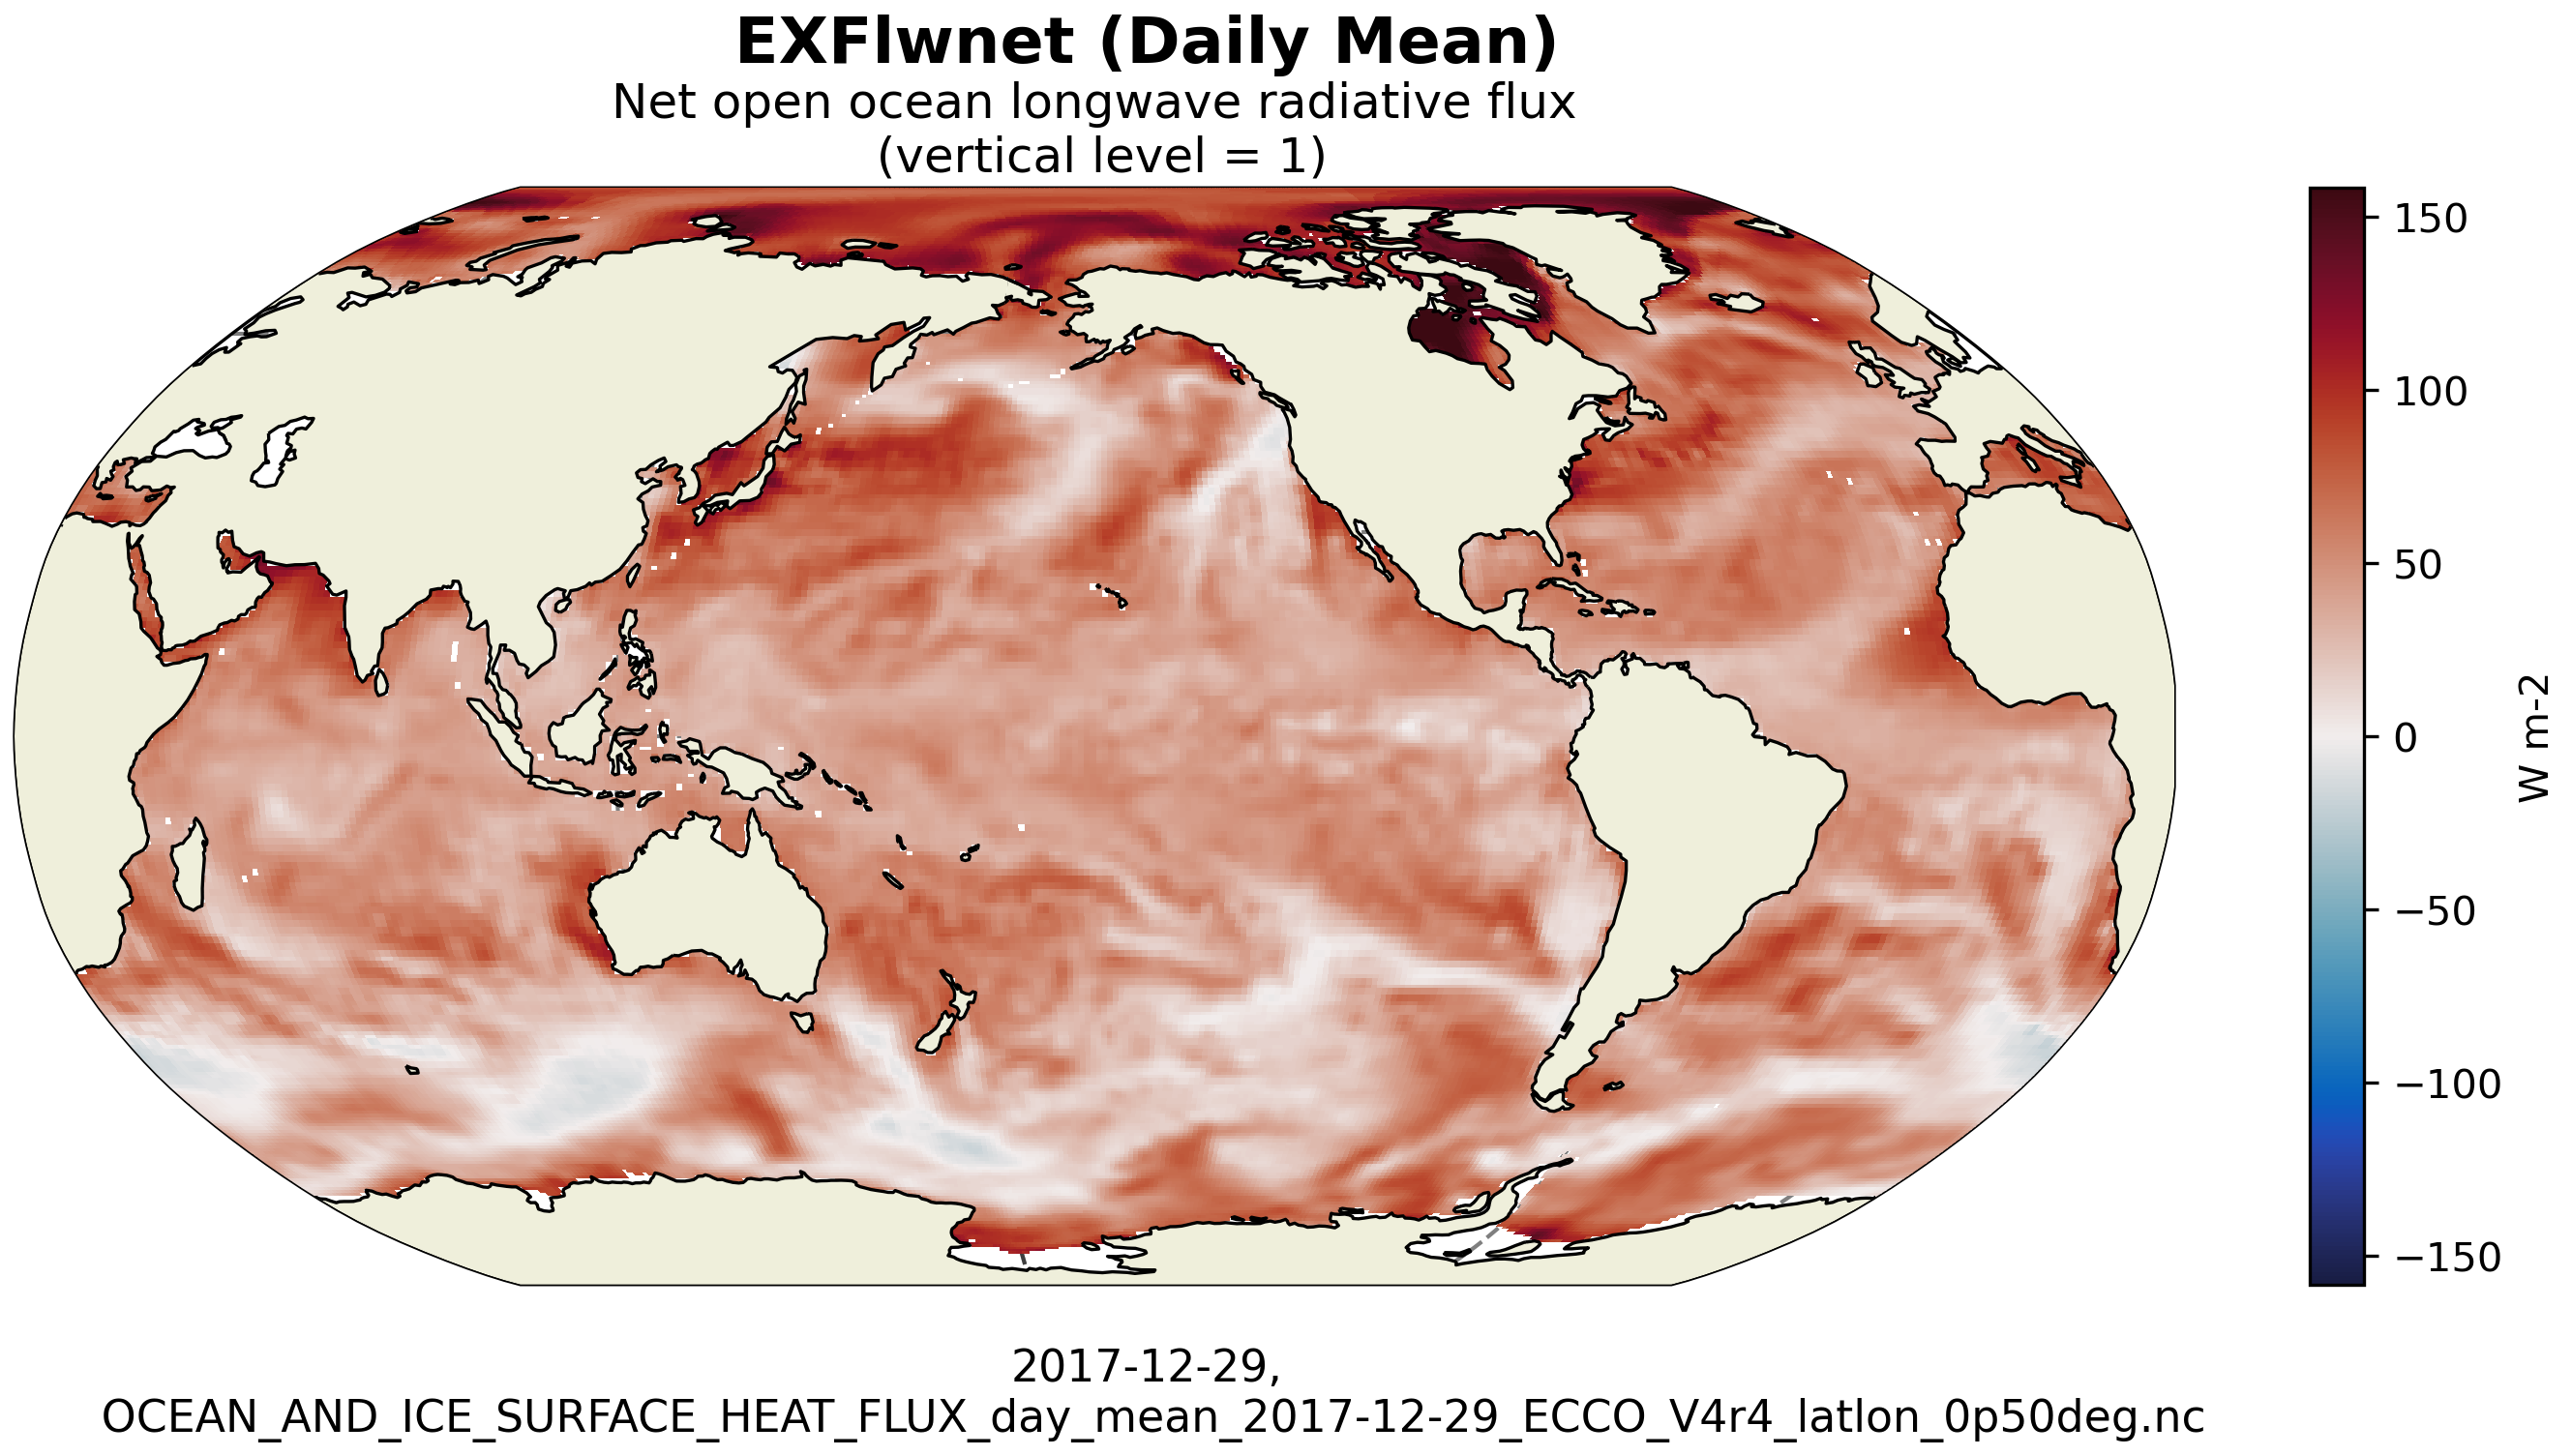
\includegraphics[scale=0.55]{../images/plots/v4r4/latlon_plots/Ocean_and_Sea-Ice_Surface_Heat_Fluxes/EXFlwnet.png}
\caption{Dataset: OCEAN\_AND\_ICE\_SURFACE\_HEAT\_FLUX, Variable: EXFlwnet}
\label{tab:table-OCEAN_AND_ICE_SURFACE_HEAT_FLUX_EXFlwnet-Plot}
\end{figure}
\newpage
\pagebreak
\subsubsection{Latlon Variable: EXFqnet}
\begin{longtable}{|m{0.06\textwidth}|m{0.3\textwidth}|m{0.45\textwidth}|m{0.12\textwidth}|}
\caption{Attributes description of the variable 'EXFqnet' from OCEAN\_AND\_ICE\_SURFACE\_HEAT\_FLUX's  dataset.}
\label{tab:table-OCEAN_AND_ICE_SURFACE_HEAT_FLUX_EXFqnet} \\ 
\hline \endhead \hline \endfoot
\rowcolor{lightgray} \textbf{Storage Type} & \textbf{Variable Name} & \textbf{Description} & \textbf{Unit} \\ \hline
float32 & EXFqnet & Open ocean net air-sea heat flux & W m-2 \\ \hline
\multicolumn{4}{|c|}{\cellcolor{lightgray}{\textbf{Description of the variable in Common Data language (CDL)}}} \\ \hline
\multicolumn{4}{|c|}{\fontfamily{lmtt}\selectfont{\makecell{\parbox{.95\textwidth}{\vspace*{0.25cm} \footnotesize{float32 EXFqnet(time, latitude, longitude)\\
\hspace*{0.5cm}EXFqnet: \_FillValue = 9.96921e+36\\
\hspace*{0.5cm}EXFqnet: coordinates = time\\
\hspace*{0.5cm}EXFqnet: coverage\_content\_type = modelResult\\
\hspace*{0.5cm}EXFqnet: direction = >0 increases potential temperature (THETA)\\
\hspace*{0.5cm}EXFqnet: long\_name = Open ocean net air-sea heat flux\\
\hspace*{0.5cm}EXFqnet: units = W m-2\\
\hspace*{0.5cm}EXFqnet: valid\_max = 3408.977783203125\\
\hspace*{0.5cm}EXFqnet: valid\_min = -687.8736572265625\\
}}}}} \\ \hline
\rowcolor{lightgray} \multicolumn{4}{|c|}{\textbf{Comments}} \\ \hline
\multicolumn{4}{|p{1\textwidth}|}{\footnotesize{{Net air-sea heat flux (turbulent and radiative) per unit area of open water (not covered by sea-ice). note: net upward heat flux over open water, calculated as exflwnet+exfswnet-exflh-exfhs.}}} \\ \hline
\end{longtable}

\begin{figure}[H]
\centering
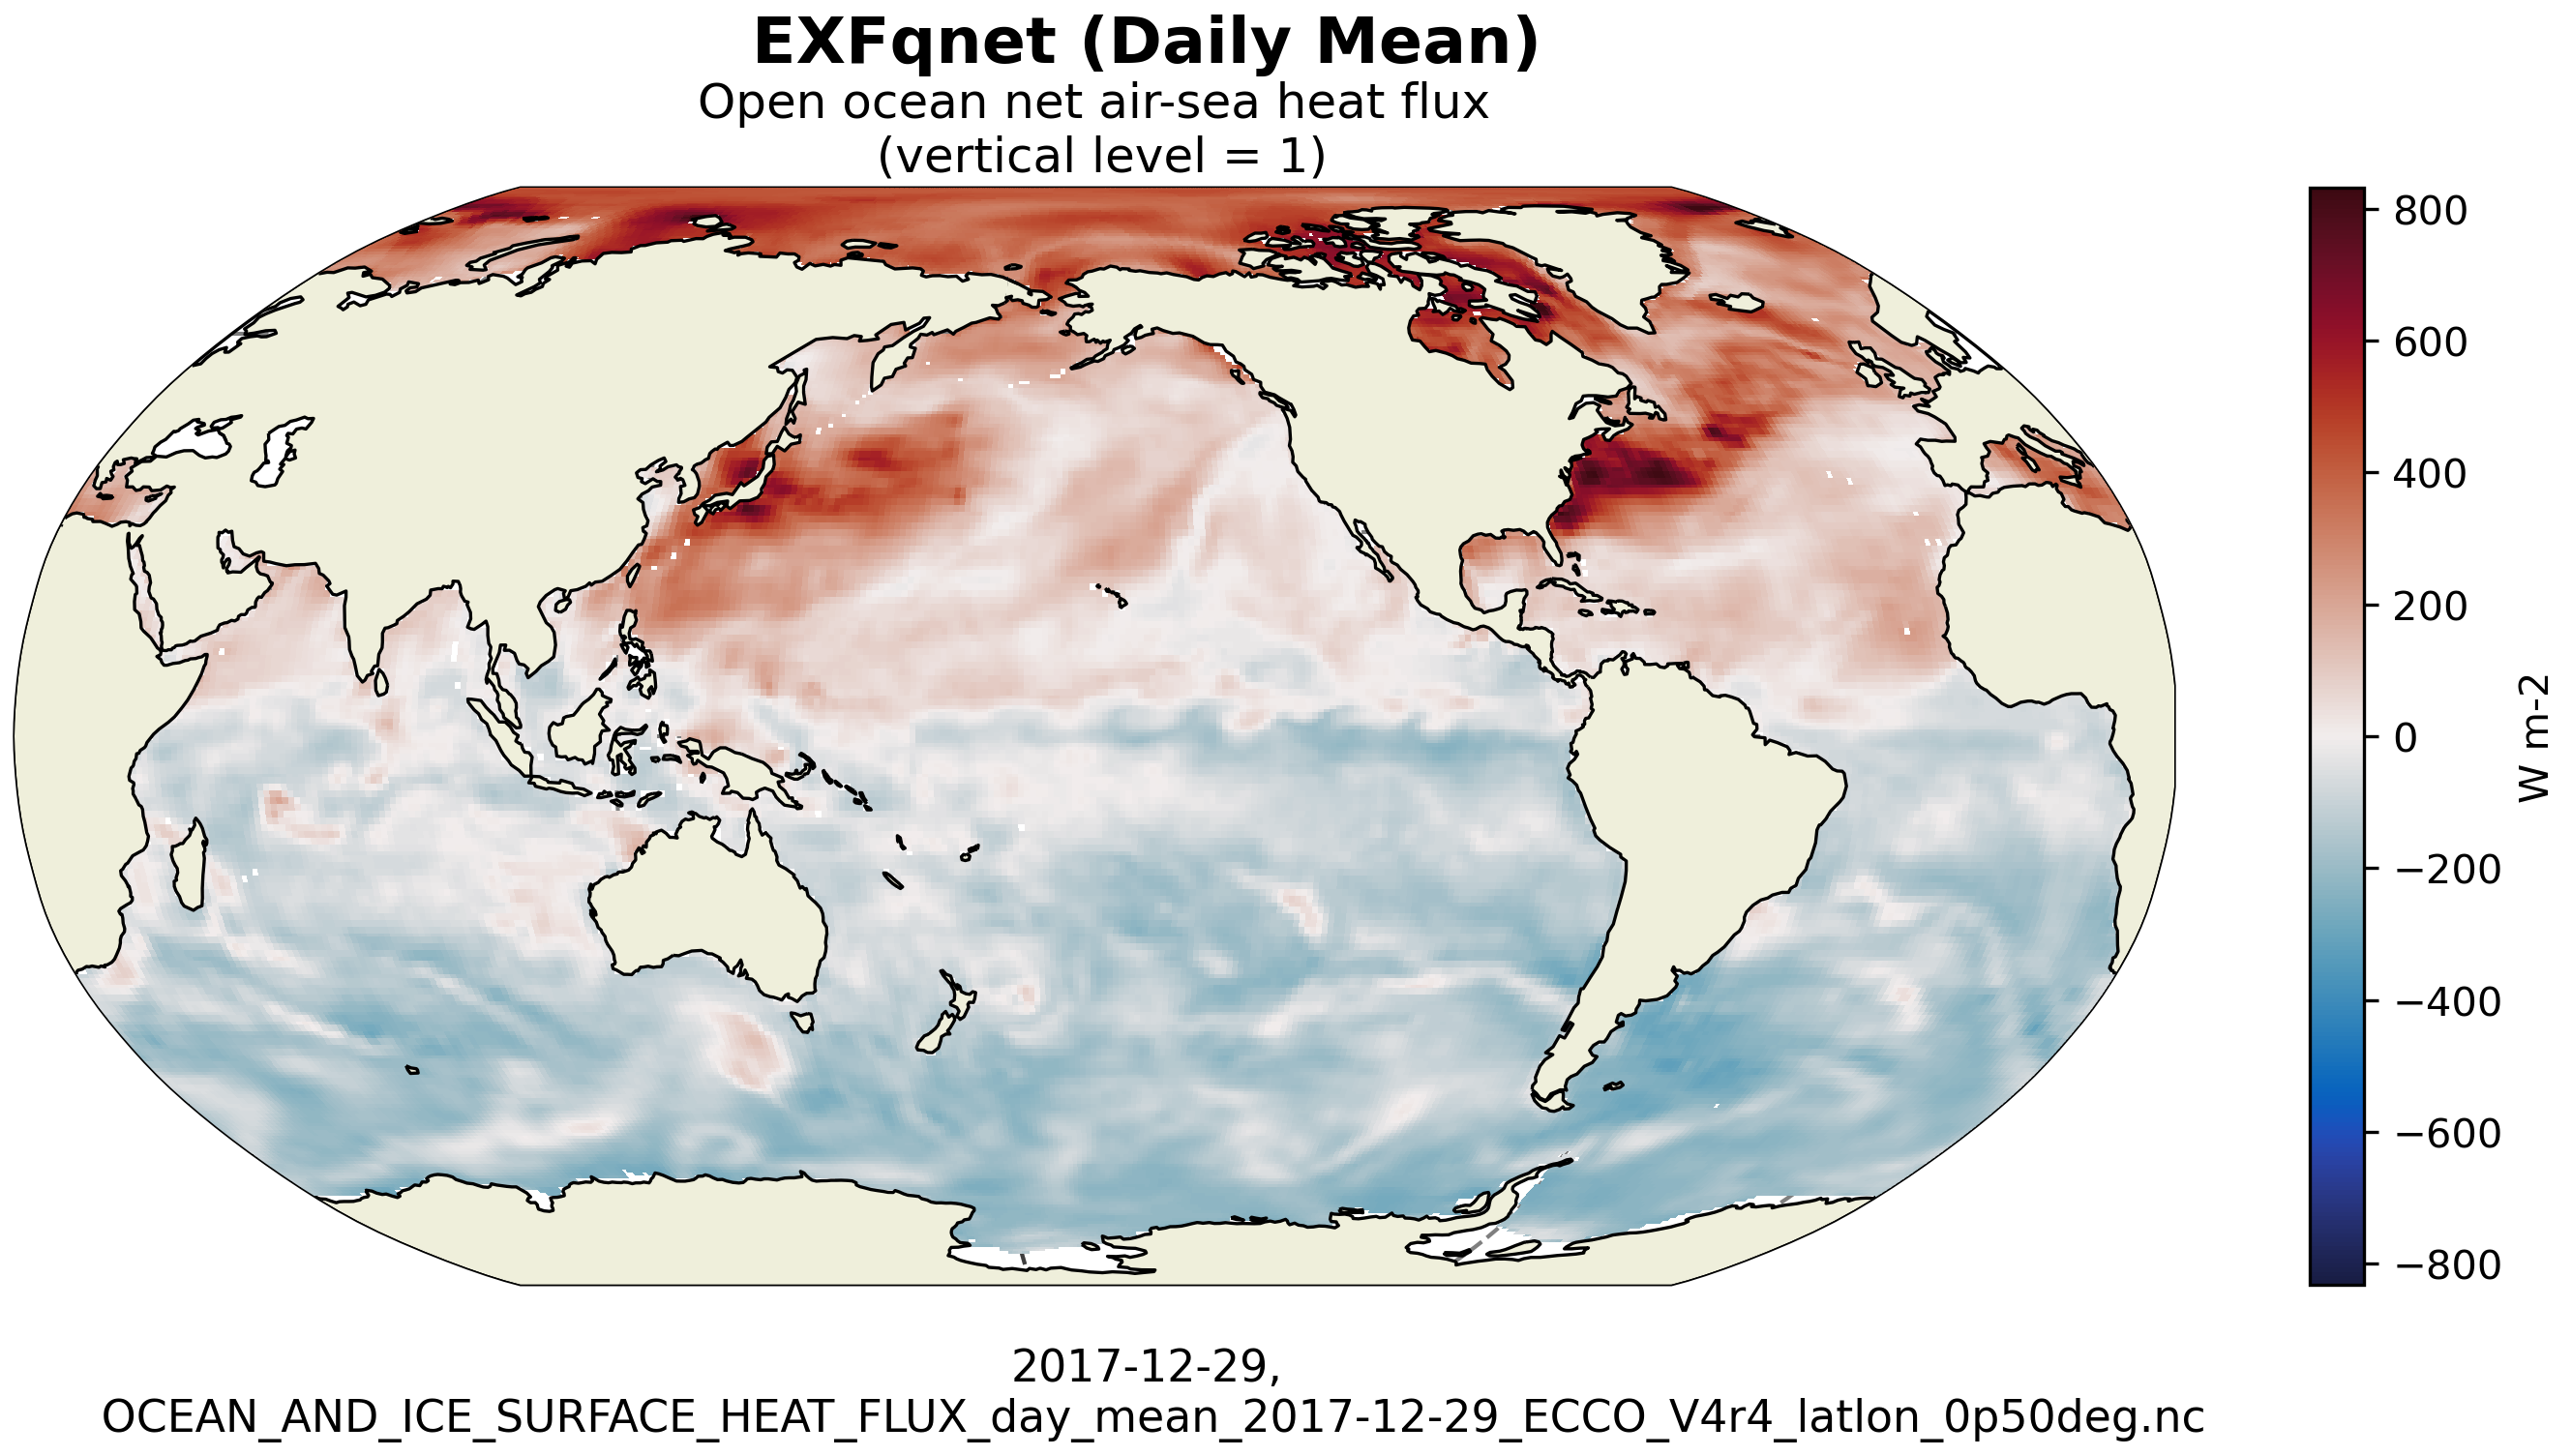
\includegraphics[scale=0.55]{../images/plots/v4r4/latlon_plots/Ocean_and_Sea-Ice_Surface_Heat_Fluxes/EXFqnet.png}
\caption{Dataset: OCEAN\_AND\_ICE\_SURFACE\_HEAT\_FLUX, Variable: EXFqnet}
\label{tab:table-OCEAN_AND_ICE_SURFACE_HEAT_FLUX_EXFqnet-Plot}
\end{figure}
\newpage
\pagebreak
\subsubsection{Latlon Variable: EXFswdn}
\begin{longtable}{|m{0.06\textwidth}|m{0.3\textwidth}|m{0.45\textwidth}|m{0.12\textwidth}|}
\caption{Attributes description of the variable 'EXFswdn' from OCEAN\_AND\_ICE\_SURFACE\_HEAT\_FLUX's  dataset.}
\label{tab:table-OCEAN_AND_ICE_SURFACE_HEAT_FLUX_EXFswdn} \\ 
\hline \endhead \hline \endfoot
\rowcolor{lightgray} \textbf{Storage Type} & \textbf{Variable Name} & \textbf{Description} & \textbf{Unit} \\ \hline
float32 & EXFswdn & Downwelling shortwave radiative flux & W m-2 \\ \hline
\multicolumn{4}{|c|}{\cellcolor{lightgray}{\textbf{Description of the variable in Common Data language (CDL)}}} \\ \hline
\multicolumn{4}{|c|}{\fontfamily{lmtt}\selectfont{\makecell{\parbox{.95\textwidth}{\vspace*{0.25cm} \footnotesize{float32 EXFswdn(time, latitude, longitude)\\
\hspace*{0.5cm}EXFswdn: \_FillValue = 9.96921e+36\\
\hspace*{0.5cm}EXFswdn: coordinates = time\\
\hspace*{0.5cm}EXFswdn: coverage\_content\_type = modelResult\\
\hspace*{0.5cm}EXFswdn: direction = >0 increases potential temperature (THETA)\\
\hspace*{0.5cm}EXFswdn: long\_name = Downwelling shortwave radiative flux\\
\hspace*{0.5cm}EXFswdn: standard\_name = surface downwelling shortwave flux in air\\
\hspace*{0.5cm}EXFswdn: units = W m-2\\
\hspace*{0.5cm}EXFswdn: valid\_max = 707.345947265625\\
\hspace*{0.5cm}EXFswdn: valid\_min = -224.63368225097656\\
}}}}} \\ \hline
\rowcolor{lightgray} \multicolumn{4}{|c|}{\textbf{Comments}} \\ \hline
\multicolumn{4}{|p{1\textwidth}|}{\footnotesize{{Downward shortwave radiative flux. note: sum of era-interim downward shortwave radiation and the control adjustment from ocean state estimation.}}} \\ \hline
\end{longtable}

\begin{figure}[H]
\centering
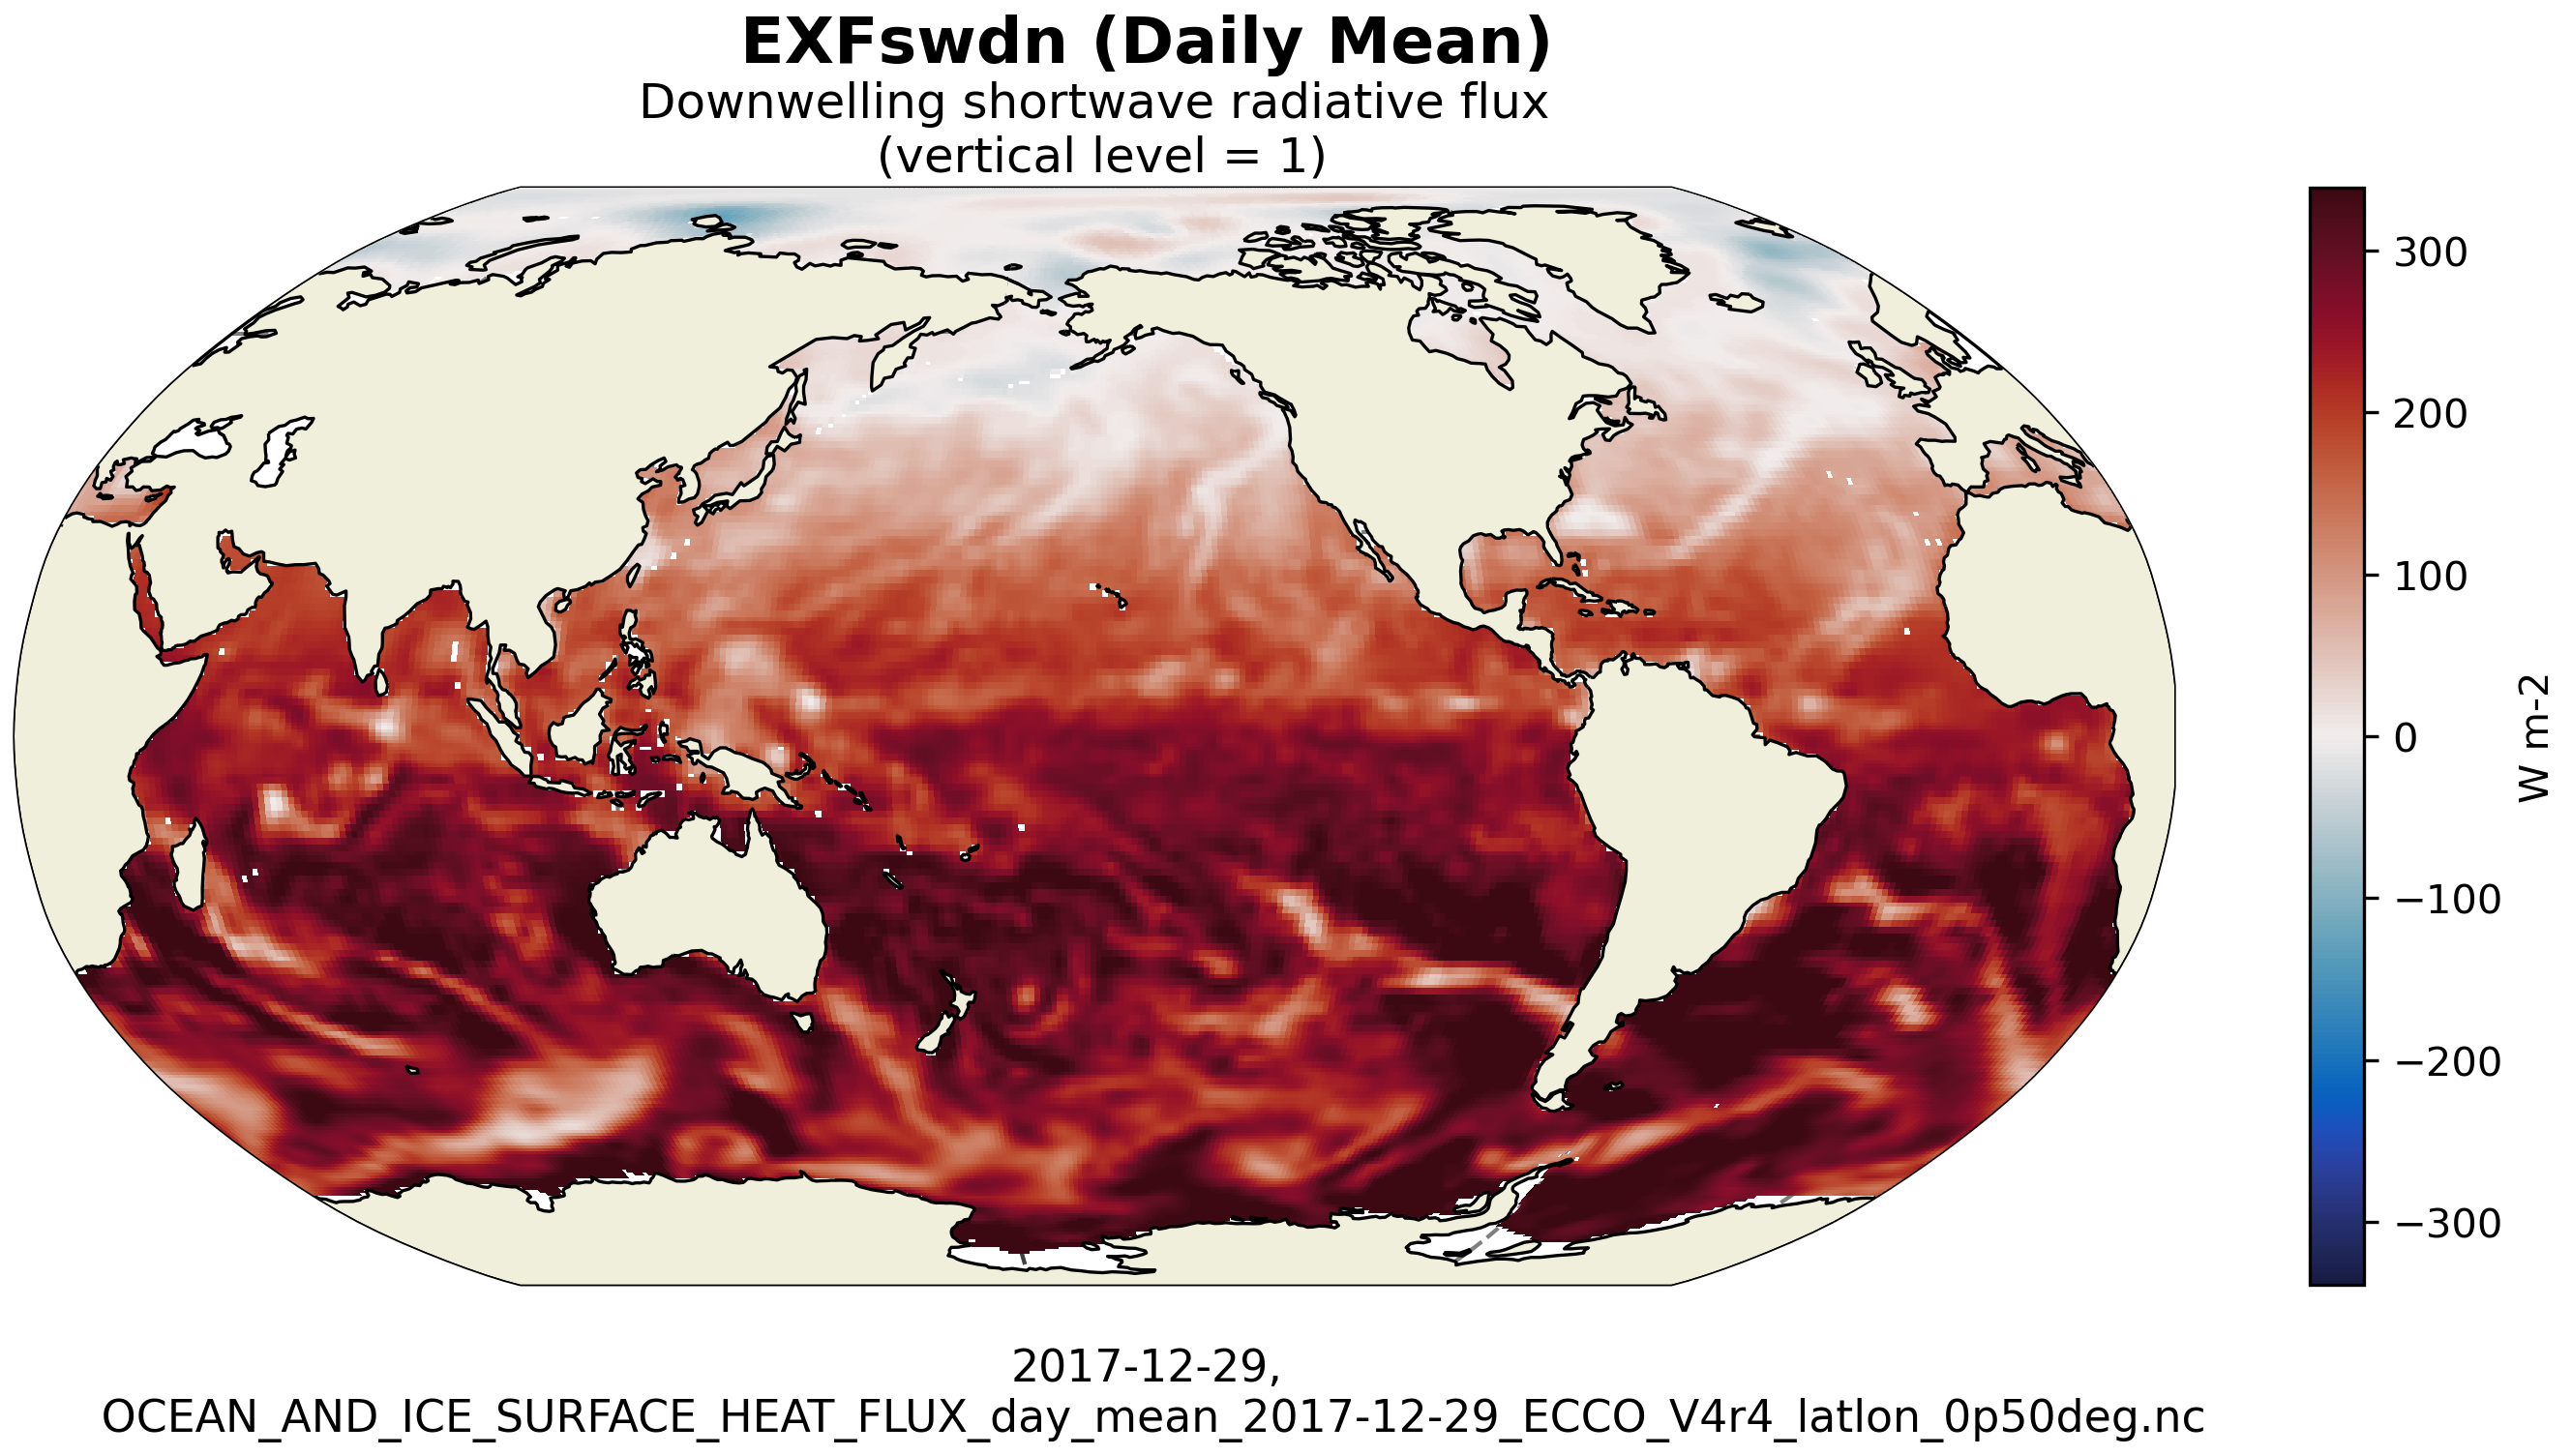
\includegraphics[scale=0.55]{../images/plots/v4r4/latlon_plots/Ocean_and_Sea-Ice_Surface_Heat_Fluxes/EXFswdn.png}
\caption{Dataset: OCEAN\_AND\_ICE\_SURFACE\_HEAT\_FLUX, Variable: EXFswdn}
\label{tab:table-OCEAN_AND_ICE_SURFACE_HEAT_FLUX_EXFswdn-Plot}
\end{figure}
\newpage
\pagebreak
\subsubsection{Latlon Variable: EXFswnet}
\begin{longtable}{|m{0.06\textwidth}|m{0.3\textwidth}|m{0.45\textwidth}|m{0.12\textwidth}|}
\caption{Attributes description of the variable 'EXFswnet' from OCEAN\_AND\_ICE\_SURFACE\_HEAT\_FLUX's  dataset.}
\label{tab:table-OCEAN_AND_ICE_SURFACE_HEAT_FLUX_EXFswnet} \\ 
\hline \endhead \hline \endfoot
\rowcolor{lightgray} \textbf{Storage Type} & \textbf{Variable Name} & \textbf{Description} & \textbf{Unit} \\ \hline
float32 & EXFswnet & Open ocean net shortwave radiative flux & W m-2 \\ \hline
\multicolumn{4}{|c|}{\cellcolor{lightgray}{\textbf{Description of the variable in Common Data language (CDL)}}} \\ \hline
\multicolumn{4}{|c|}{\fontfamily{lmtt}\selectfont{\makecell{\parbox{.95\textwidth}{\vspace*{0.25cm} \footnotesize{float32 EXFswnet(time, latitude, longitude)\\
\hspace*{0.5cm}EXFswnet: \_FillValue = 9.96921e+36\\
\hspace*{0.5cm}EXFswnet: coordinates = time\\
\hspace*{0.5cm}EXFswnet: coverage\_content\_type = modelResult\\
\hspace*{0.5cm}EXFswnet: direction = >0 increases potential temperature (THETA)\\
\hspace*{0.5cm}EXFswnet: long\_name = Open ocean net shortwave radiative flux\\
\hspace*{0.5cm}EXFswnet: standard\_name = surface net downward shortwave flux\\
\hspace*{0.5cm}EXFswnet: units = W m-2\\
\hspace*{0.5cm}EXFswnet: valid\_max = 193.89297485351562\\
\hspace*{0.5cm}EXFswnet: valid\_min = -655.6171264648438\\
}}}}} \\ \hline
\rowcolor{lightgray} \multicolumn{4}{|c|}{\textbf{Comments}} \\ \hline
\multicolumn{4}{|p{1\textwidth}|}{\footnotesize{{Net shortwave radiative flux per unit area of open water (not covered by sea-ice). note: net shortwave radiation over open water calculated from downward shortwave flux (exfswdn) and ocean surface albdeo.}}} \\ \hline
\end{longtable}

\begin{figure}[H]
\centering
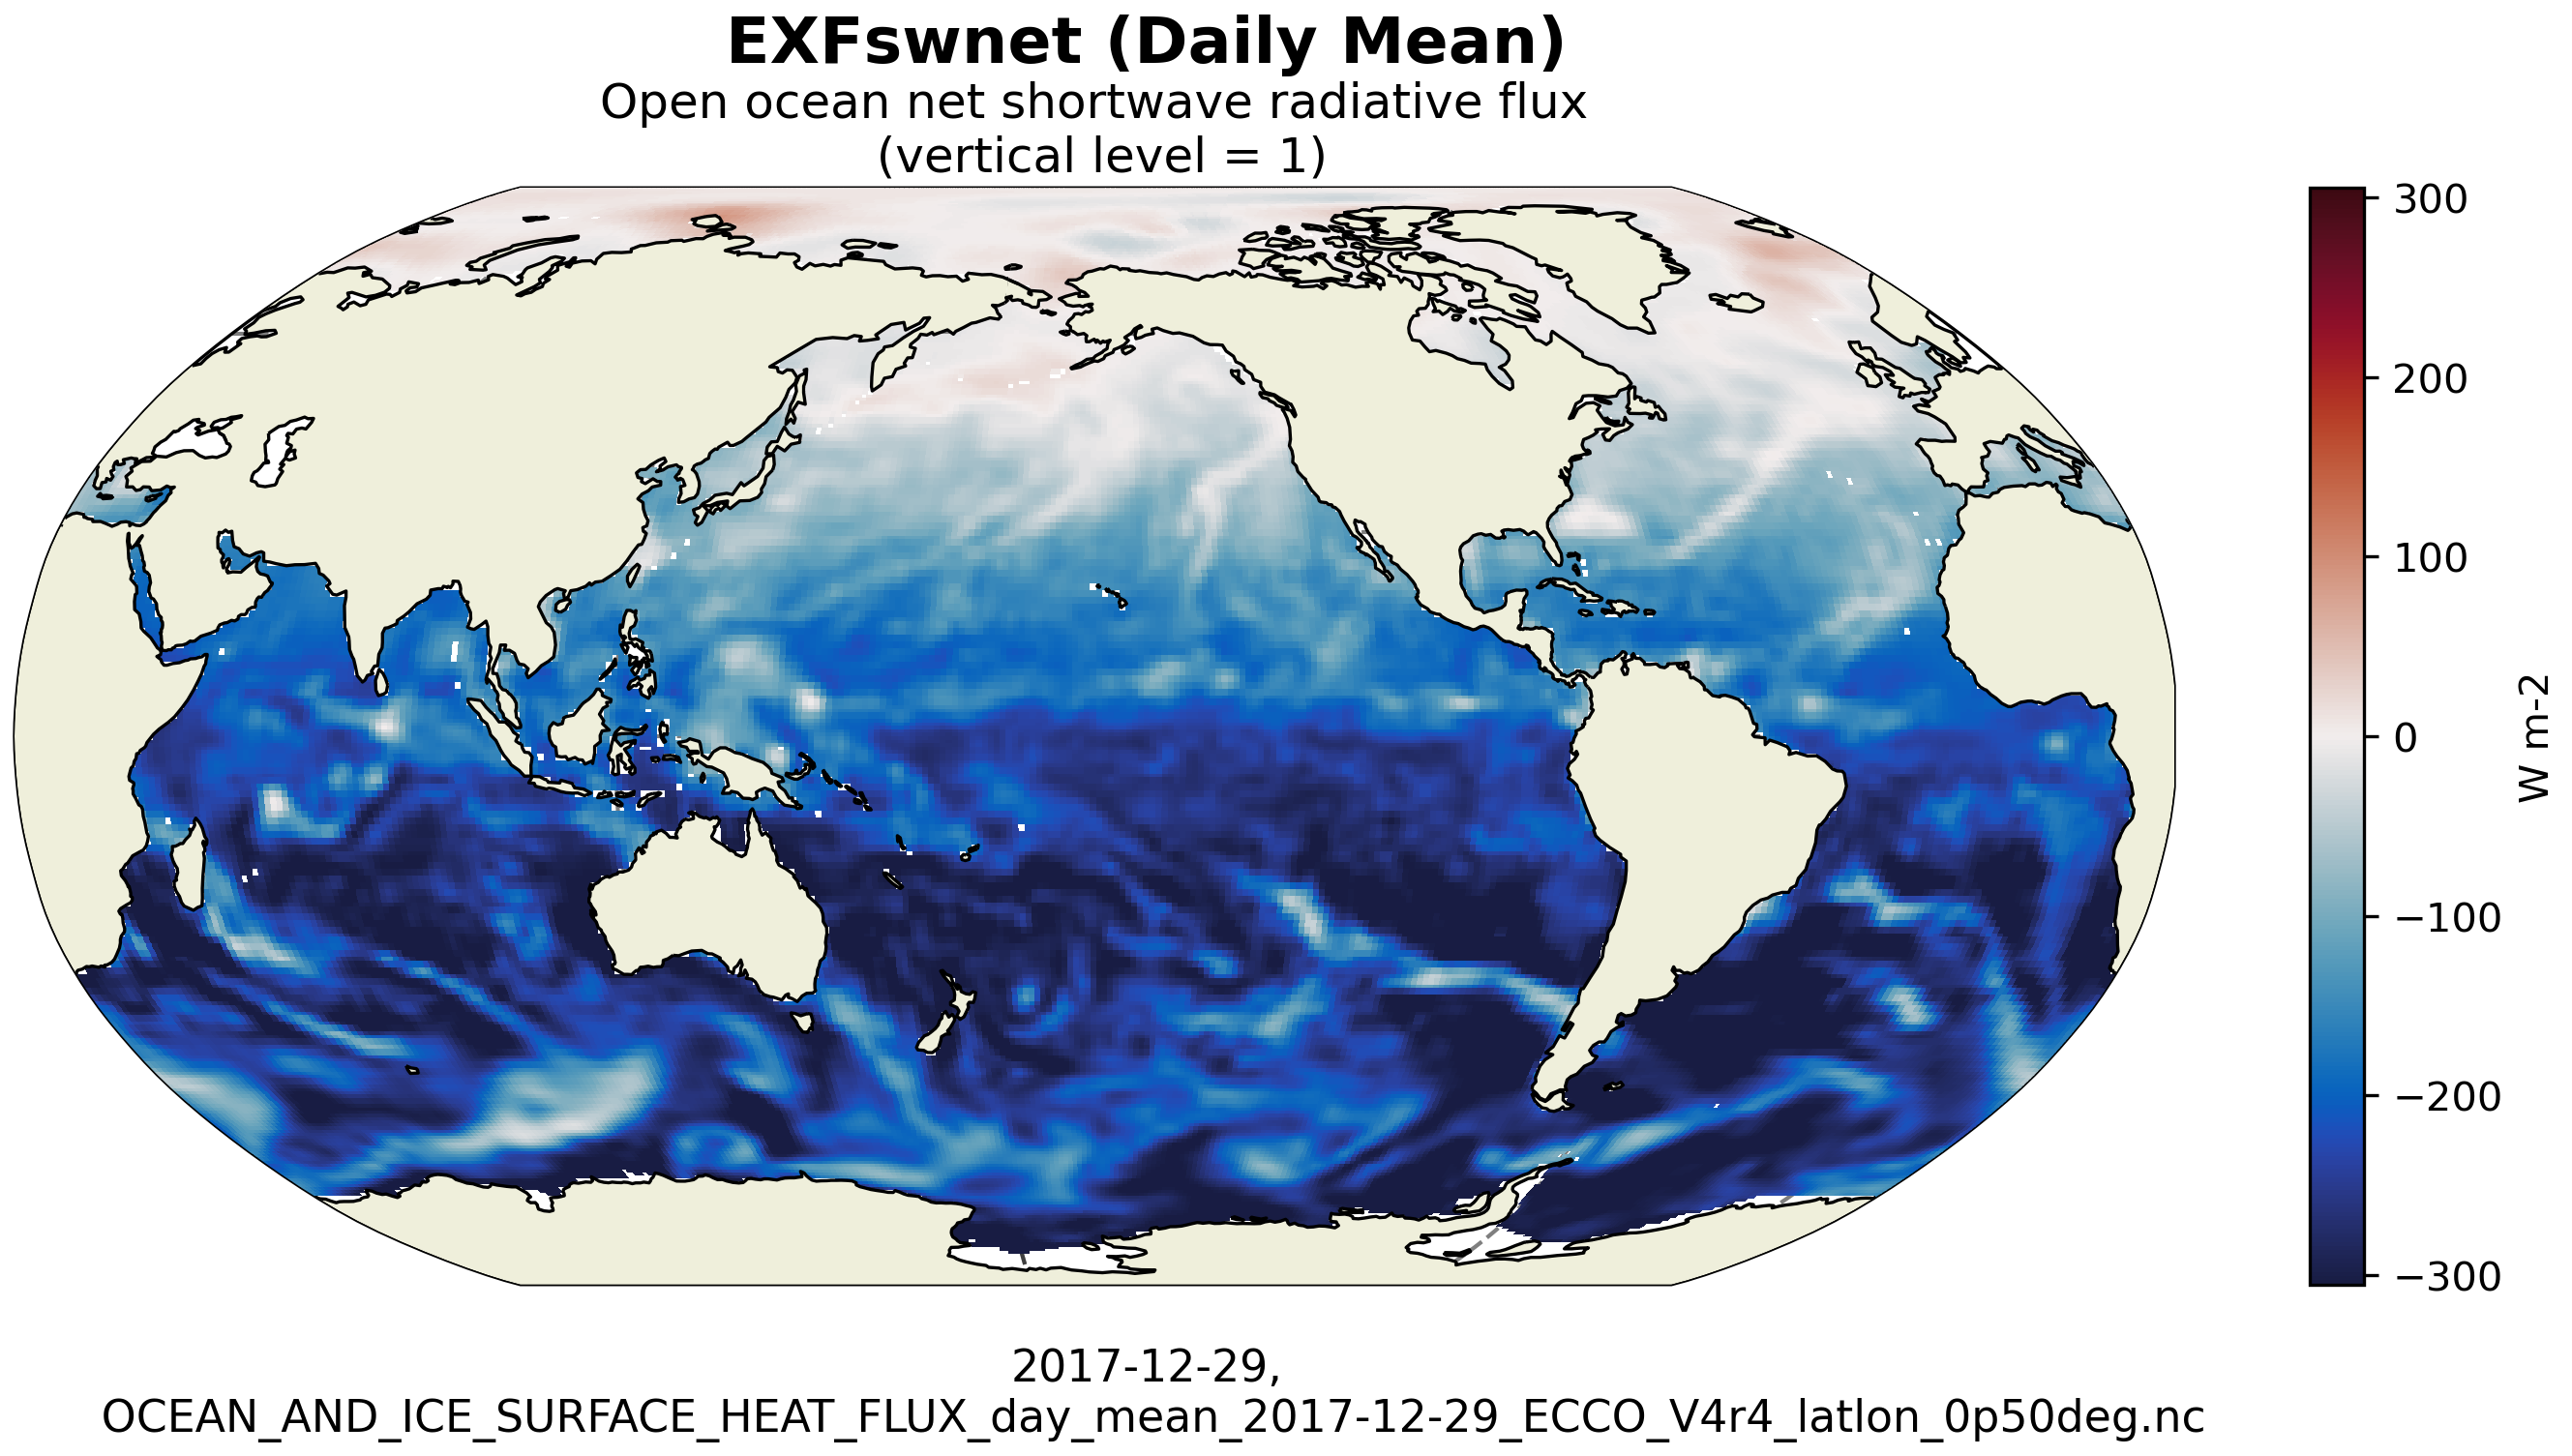
\includegraphics[scale=0.55]{../images/plots/v4r4/latlon_plots/Ocean_and_Sea-Ice_Surface_Heat_Fluxes/EXFswnet.png}
\caption{Dataset: OCEAN\_AND\_ICE\_SURFACE\_HEAT\_FLUX, Variable: EXFswnet}
\label{tab:table-OCEAN_AND_ICE_SURFACE_HEAT_FLUX_EXFswnet-Plot}
\end{figure}
\newpage
\pagebreak
\subsubsection{Latlon Variable: SIaaflux}
\begin{longtable}{|m{0.06\textwidth}|m{0.3\textwidth}|m{0.45\textwidth}|m{0.12\textwidth}|}
\caption{Attributes description of the variable 'SIaaflux' from OCEAN\_AND\_ICE\_SURFACE\_HEAT\_FLUX's  dataset.}
\label{tab:table-OCEAN_AND_ICE_SURFACE_HEAT_FLUX_SIaaflux} \\ 
\hline \endhead \hline \endfoot
\rowcolor{lightgray} \textbf{Storage Type} & \textbf{Variable Name} & \textbf{Description} & \textbf{Unit} \\ \hline
float32 & SIaaflux & Conservative ocean and sea-ice advective heat flux adjustment & W m-2 \\ \hline
\multicolumn{4}{|c|}{\cellcolor{lightgray}{\textbf{Description of the variable in Common Data language (CDL)}}} \\ \hline
\multicolumn{4}{|c|}{\fontfamily{lmtt}\selectfont{\makecell{\parbox{.95\textwidth}{\vspace*{0.25cm} \footnotesize{float32 SIaaflux(time, latitude, longitude)\\
\hspace*{0.5cm}SIaaflux: \_FillValue = 9.96921e+36\\
\hspace*{0.5cm}SIaaflux: coordinates = time\\
\hspace*{0.5cm}SIaaflux: coverage\_content\_type = modelResult\\
\hspace*{0.5cm}SIaaflux: direction = >0 decrease potential temperature (THETA)\\
\hspace*{0.5cm}SIaaflux: long\_name = Conservative ocean and sea-ice advective heat flux adjustment\\
\hspace*{0.5cm}SIaaflux: units = W m-2\\
\hspace*{0.5cm}SIaaflux: valid\_max = 50.35451889038086\\
\hspace*{0.5cm}SIaaflux: valid\_min = -16.214622497558594\\
}}}}} \\ \hline
\rowcolor{lightgray} \multicolumn{4}{|c|}{\textbf{Comments}} \\ \hline
\multicolumn{4}{|p{1\textwidth}|}{\footnotesize{{Heat flux associated with the temperature difference between sea surface temperature and sea-ice (assume 0 degree c in the model). note: heat flux needed to melt/freeze sea-ice at 0 degc to sea water at the ocean surface (at sea surface temperature), excluding the latent heat of fusion.}}} \\ \hline
\end{longtable}

\begin{figure}[H]
\centering
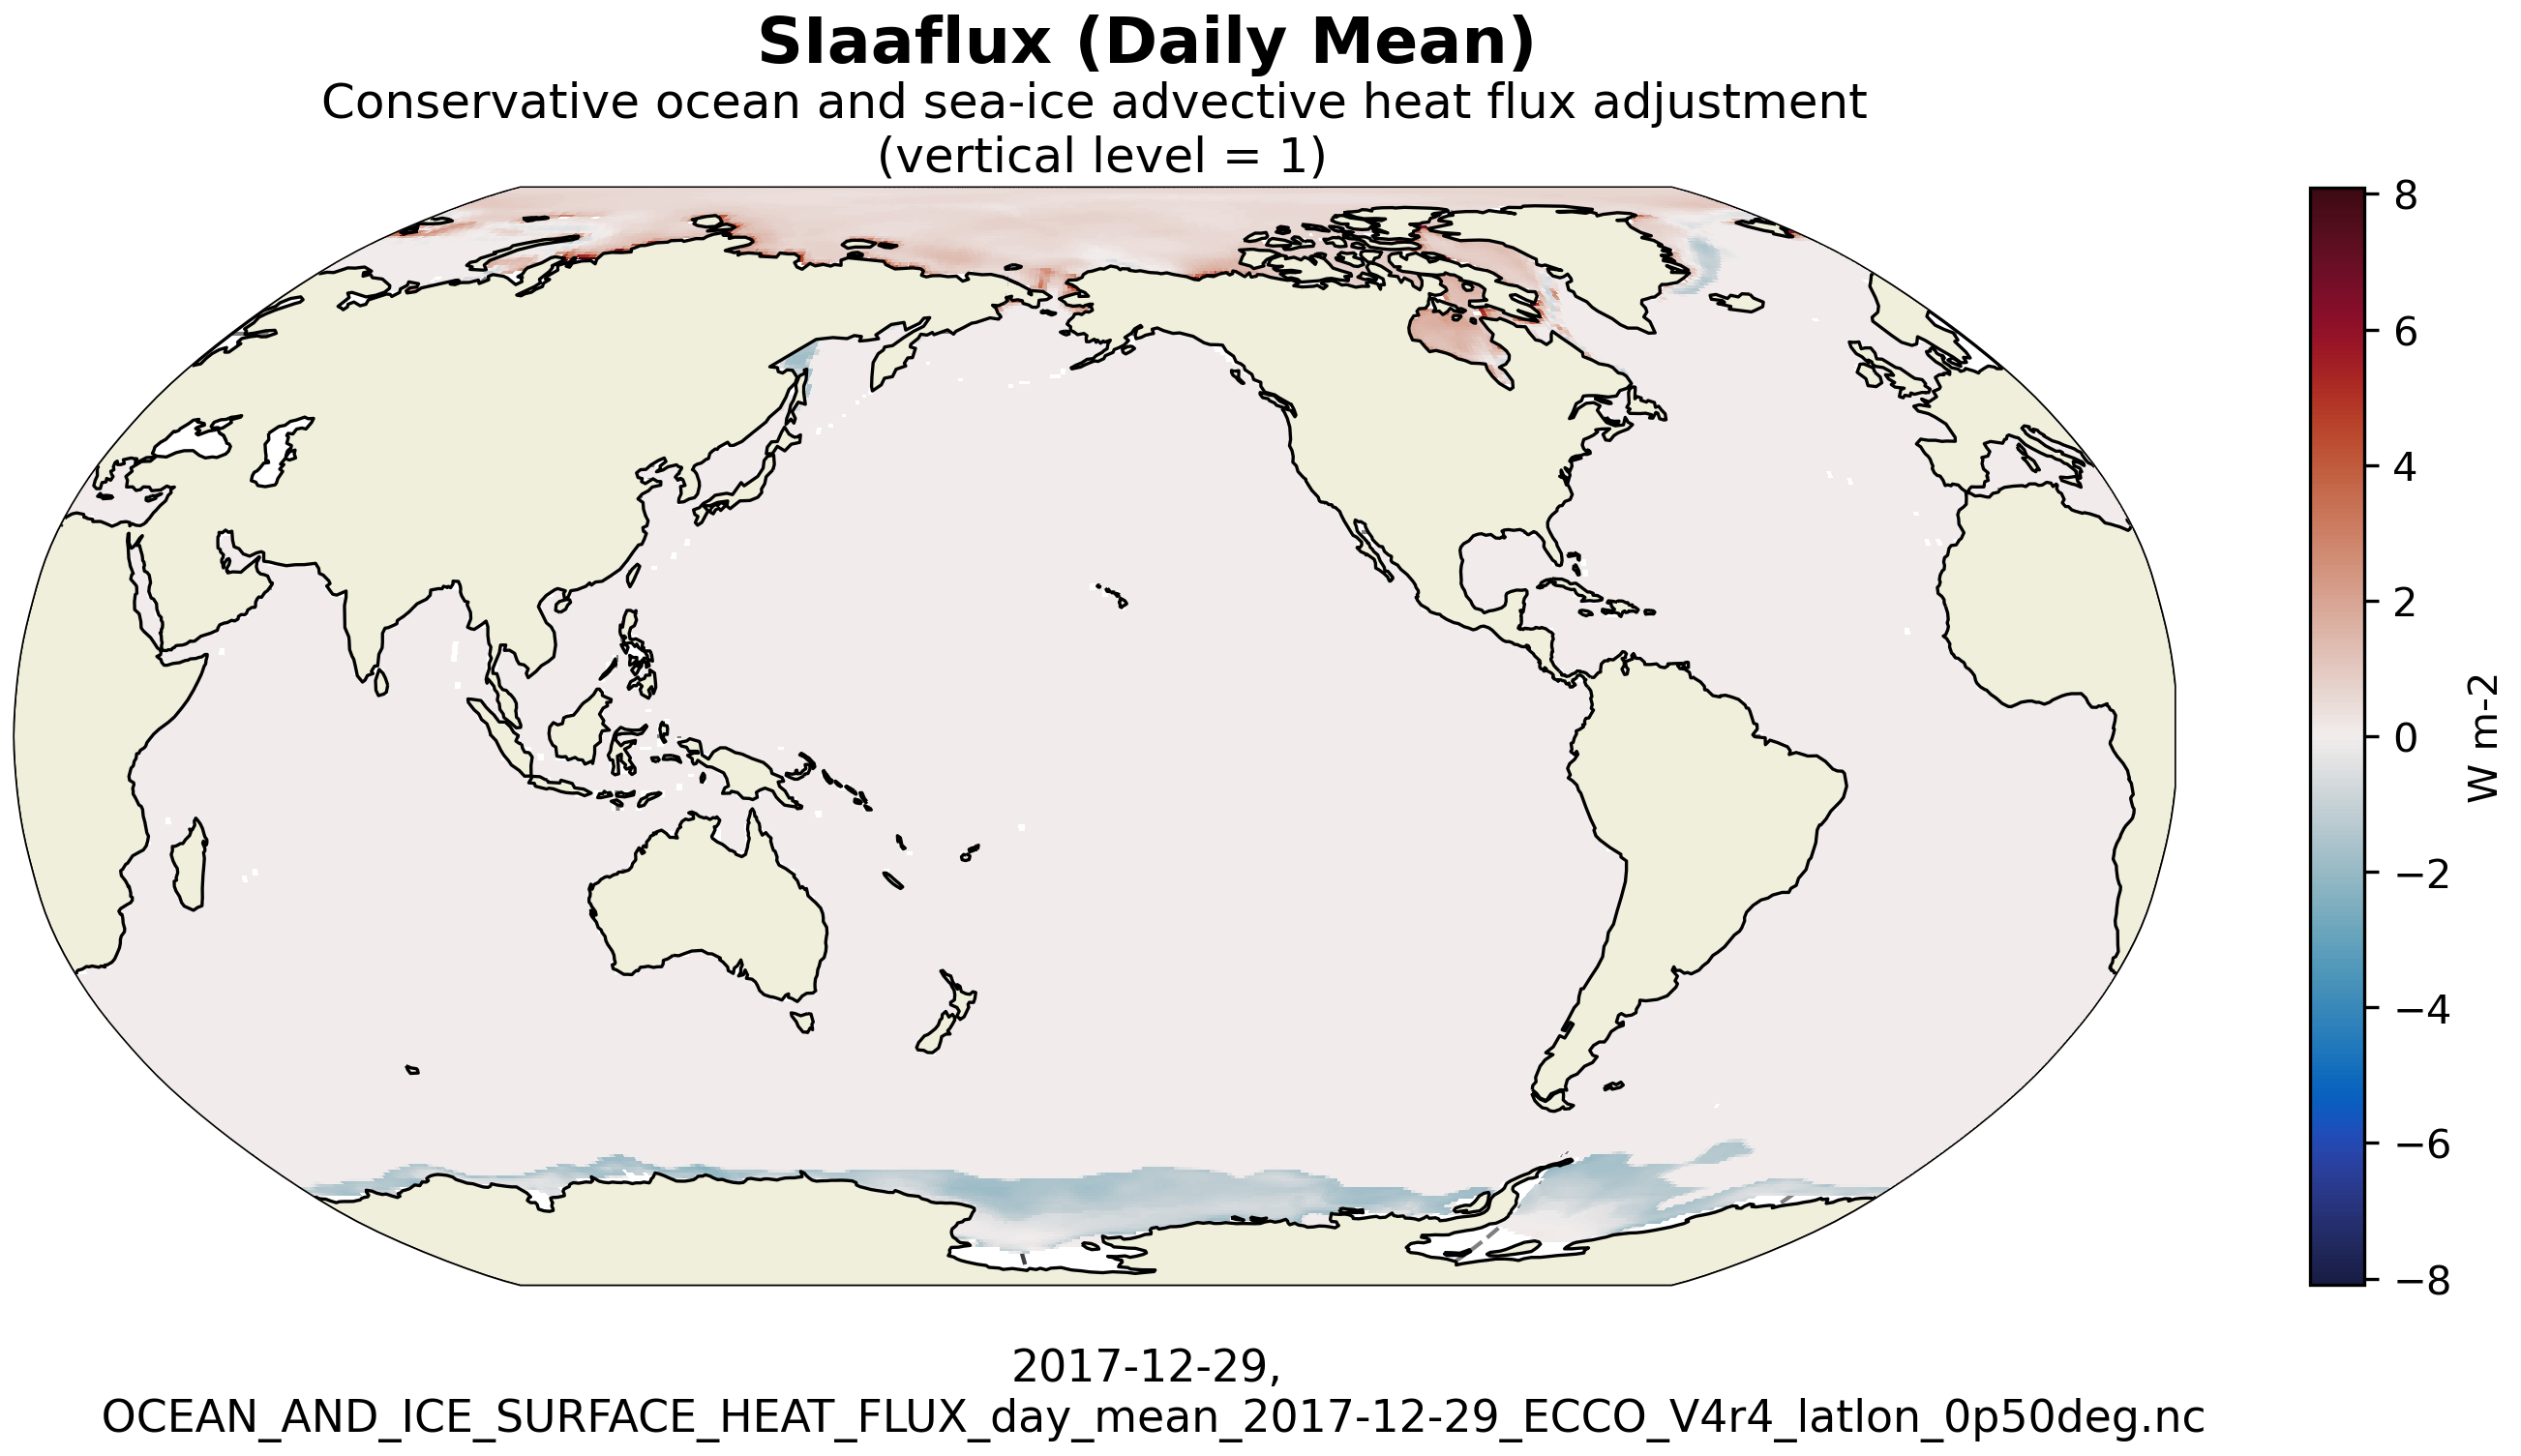
\includegraphics[scale=0.55]{../images/plots/v4r4/latlon_plots/Ocean_and_Sea-Ice_Surface_Heat_Fluxes/SIaaflux.png}
\caption{Dataset: OCEAN\_AND\_ICE\_SURFACE\_HEAT\_FLUX, Variable: SIaaflux}
\label{tab:table-OCEAN_AND_ICE_SURFACE_HEAT_FLUX_SIaaflux-Plot}
\end{figure}
\newpage
\pagebreak
\subsubsection{Latlon Variable: SIatmQnt}
\begin{longtable}{|m{0.06\textwidth}|m{0.3\textwidth}|m{0.45\textwidth}|m{0.12\textwidth}|}
\caption{Attributes description of the variable 'SIatmQnt' from OCEAN\_AND\_ICE\_SURFACE\_HEAT\_FLUX's  dataset.}
\label{tab:table-OCEAN_AND_ICE_SURFACE_HEAT_FLUX_SIatmQnt} \\ 
\hline \endhead \hline \endfoot
\rowcolor{lightgray} \textbf{Storage Type} & \textbf{Variable Name} & \textbf{Description} & \textbf{Unit} \\ \hline
float32 & SIatmQnt & Net upward heat flux to the atmosphere & W m-2 \\ \hline
\multicolumn{4}{|c|}{\cellcolor{lightgray}{\textbf{Description of the variable in Common Data language (CDL)}}} \\ \hline
\multicolumn{4}{|c|}{\fontfamily{lmtt}\selectfont{\makecell{\parbox{.95\textwidth}{\vspace*{0.25cm} \footnotesize{float32 SIatmQnt(time, latitude, longitude)\\
\hspace*{0.5cm}SIatmQnt: \_FillValue = 9.96921e+36\\
\hspace*{0.5cm}SIatmQnt: coordinates = time\\
\hspace*{0.5cm}SIatmQnt: coverage\_content\_type = modelResult\\
\hspace*{0.5cm}SIatmQnt: direction = >0 upward, decreases ocean temperature\\
\hspace*{0.5cm}SIatmQnt: long\_name = Net upward heat flux to the atmosphere\\
\hspace*{0.5cm}SIatmQnt: standard\_name = surface upward heat flux in air\\
\hspace*{0.5cm}SIatmQnt: units = W m-2\\
\hspace*{0.5cm}SIatmQnt: valid\_max = 1704.7703857421875\\
\hspace*{0.5cm}SIatmQnt: valid\_min = -756.0607299804688\\
}}}}} \\ \hline
\rowcolor{lightgray} \multicolumn{4}{|c|}{\textbf{Comments}} \\ \hline
\multicolumn{4}{|p{1\textwidth}|}{\footnotesize{{Net upward heat flux to the atmosphere across open water and sea-ice or snow surfaces. note: nonzero siatmqnt may not be associated with a change in ocean potential temperature due to sea-ice growth or melting. to calculate total ocean heat content changes use the variable tflux which also accounts for changing ocean mass (e.g. ocefwflx).}}} \\ \hline
\end{longtable}

\begin{figure}[H]
\centering
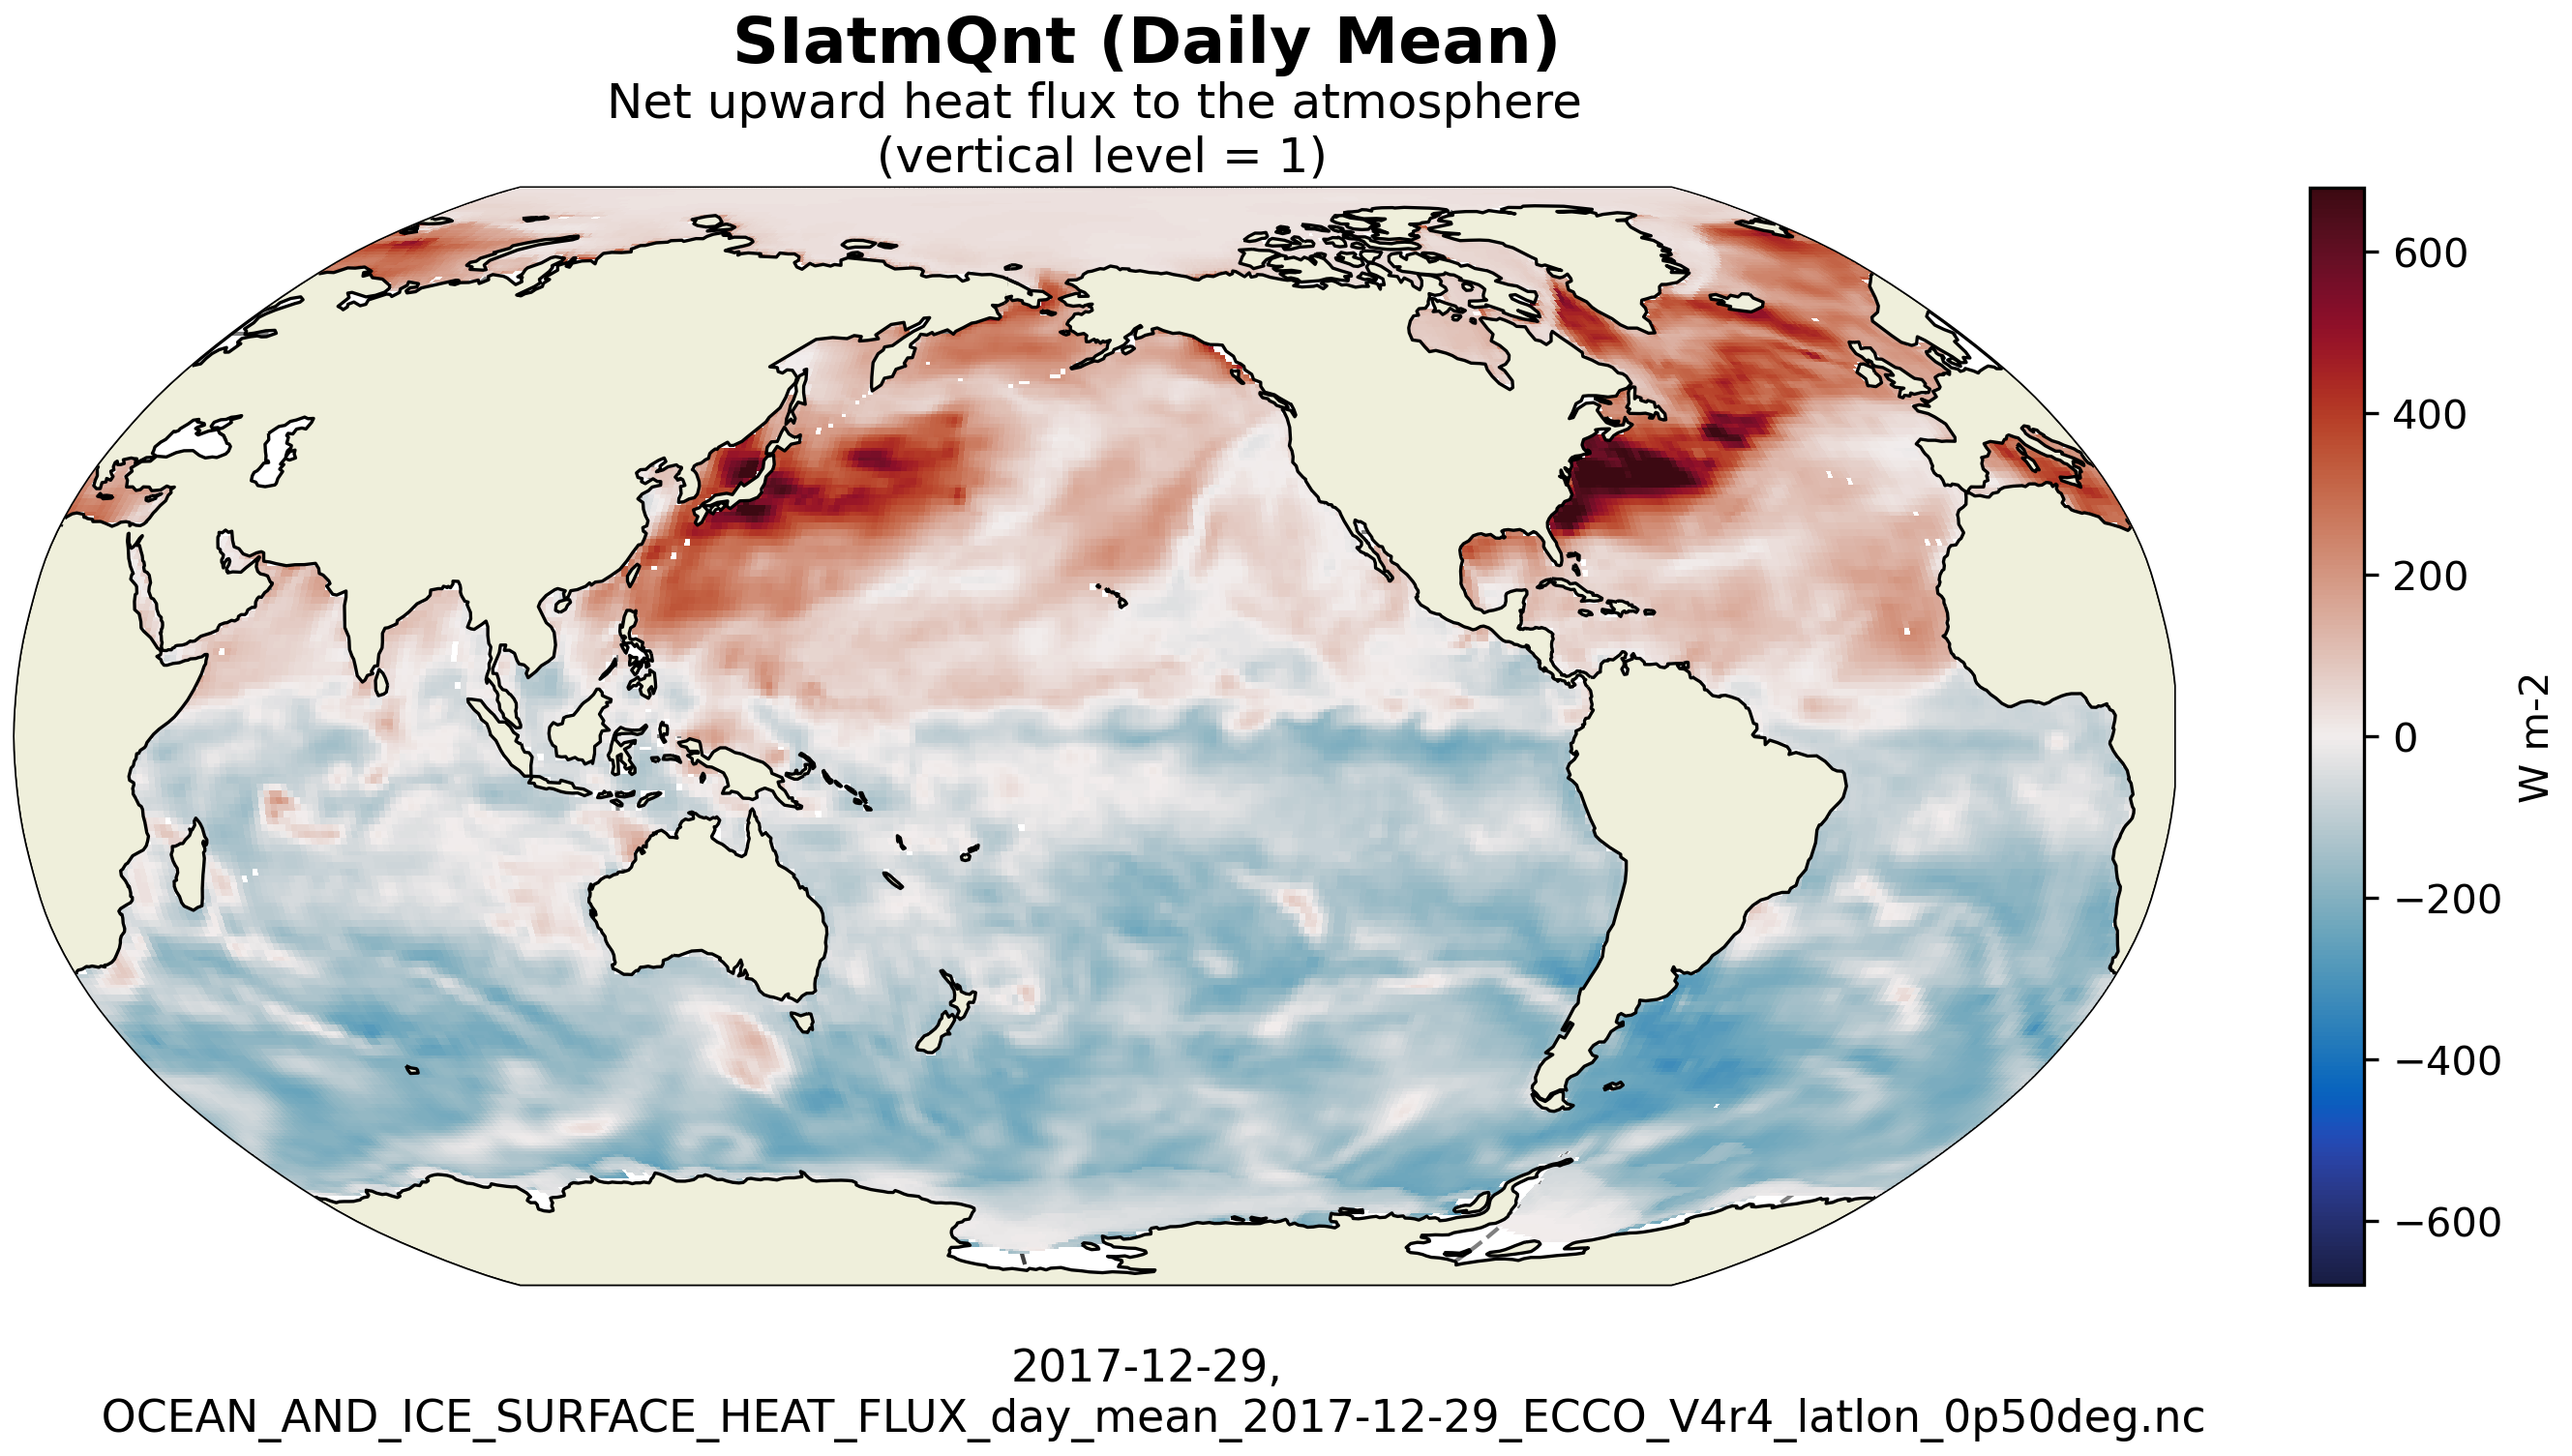
\includegraphics[scale=0.55]{../images/plots/v4r4/latlon_plots/Ocean_and_Sea-Ice_Surface_Heat_Fluxes/SIatmQnt.png}
\caption{Dataset: OCEAN\_AND\_ICE\_SURFACE\_HEAT\_FLUX, Variable: SIatmQnt}
\label{tab:table-OCEAN_AND_ICE_SURFACE_HEAT_FLUX_SIatmQnt-Plot}
\end{figure}
\newpage
\pagebreak
\subsubsection{Latlon Variable: TFLUX}
\begin{longtable}{|m{0.06\textwidth}|m{0.3\textwidth}|m{0.45\textwidth}|m{0.12\textwidth}|}
\caption{Attributes description of the variable 'TFLUX' from OCEAN\_AND\_ICE\_SURFACE\_HEAT\_FLUX's  dataset.}
\label{tab:table-OCEAN_AND_ICE_SURFACE_HEAT_FLUX_TFLUX} \\ 
\hline \endhead \hline \endfoot
\rowcolor{lightgray} \textbf{Storage Type} & \textbf{Variable Name} & \textbf{Description} & \textbf{Unit} \\ \hline
float32 & TFLUX & Rate of change of ocean heat content per m2 accounting for mass fluxes. & W m-2 \\ \hline
\multicolumn{4}{|c|}{\cellcolor{lightgray}{\textbf{Description of the variable in Common Data language (CDL)}}} \\ \hline
\multicolumn{4}{|c|}{\fontfamily{lmtt}\selectfont{\makecell{\parbox{.95\textwidth}{\vspace*{0.25cm} \footnotesize{float32 TFLUX(time, latitude, longitude)\\
\hspace*{0.5cm}TFLUX: \_FillValue = 9.96921e+36\\
\hspace*{0.5cm}TFLUX: coordinates = time\\
\hspace*{0.5cm}TFLUX: coverage\_content\_type = modelResult\\
\hspace*{0.5cm}TFLUX: direction = >0 increases potential temperature (THETA)\\
\hspace*{0.5cm}TFLUX: long\_name = Rate of change of ocean heat content per m2 accounting for mass fluxes.\\
\hspace*{0.5cm}TFLUX: units = W m-2\\
\hspace*{0.5cm}TFLUX: valid\_max = 870.3130493164062\\
\hspace*{0.5cm}TFLUX: valid\_min = -1713.51220703125\\
}}}}} \\ \hline
\rowcolor{lightgray} \multicolumn{4}{|c|}{\textbf{Comments}} \\ \hline
\multicolumn{4}{|p{1\textwidth}|}{\footnotesize{{The rate of change of ocean heat content due to heat fluxes across the liquid surface and the addition or removal of mass. . note: the global area integral of tflux and geothermal flux (geothermalflux.bin) matches the time-derivative of ocean heat content (j/s). unlike oceqnet, tflux includes the contribution to the ocean heat content from changing ocean mass (e.g. from ocefwflx).}}} \\ \hline
\end{longtable}

\begin{figure}[H]
\centering
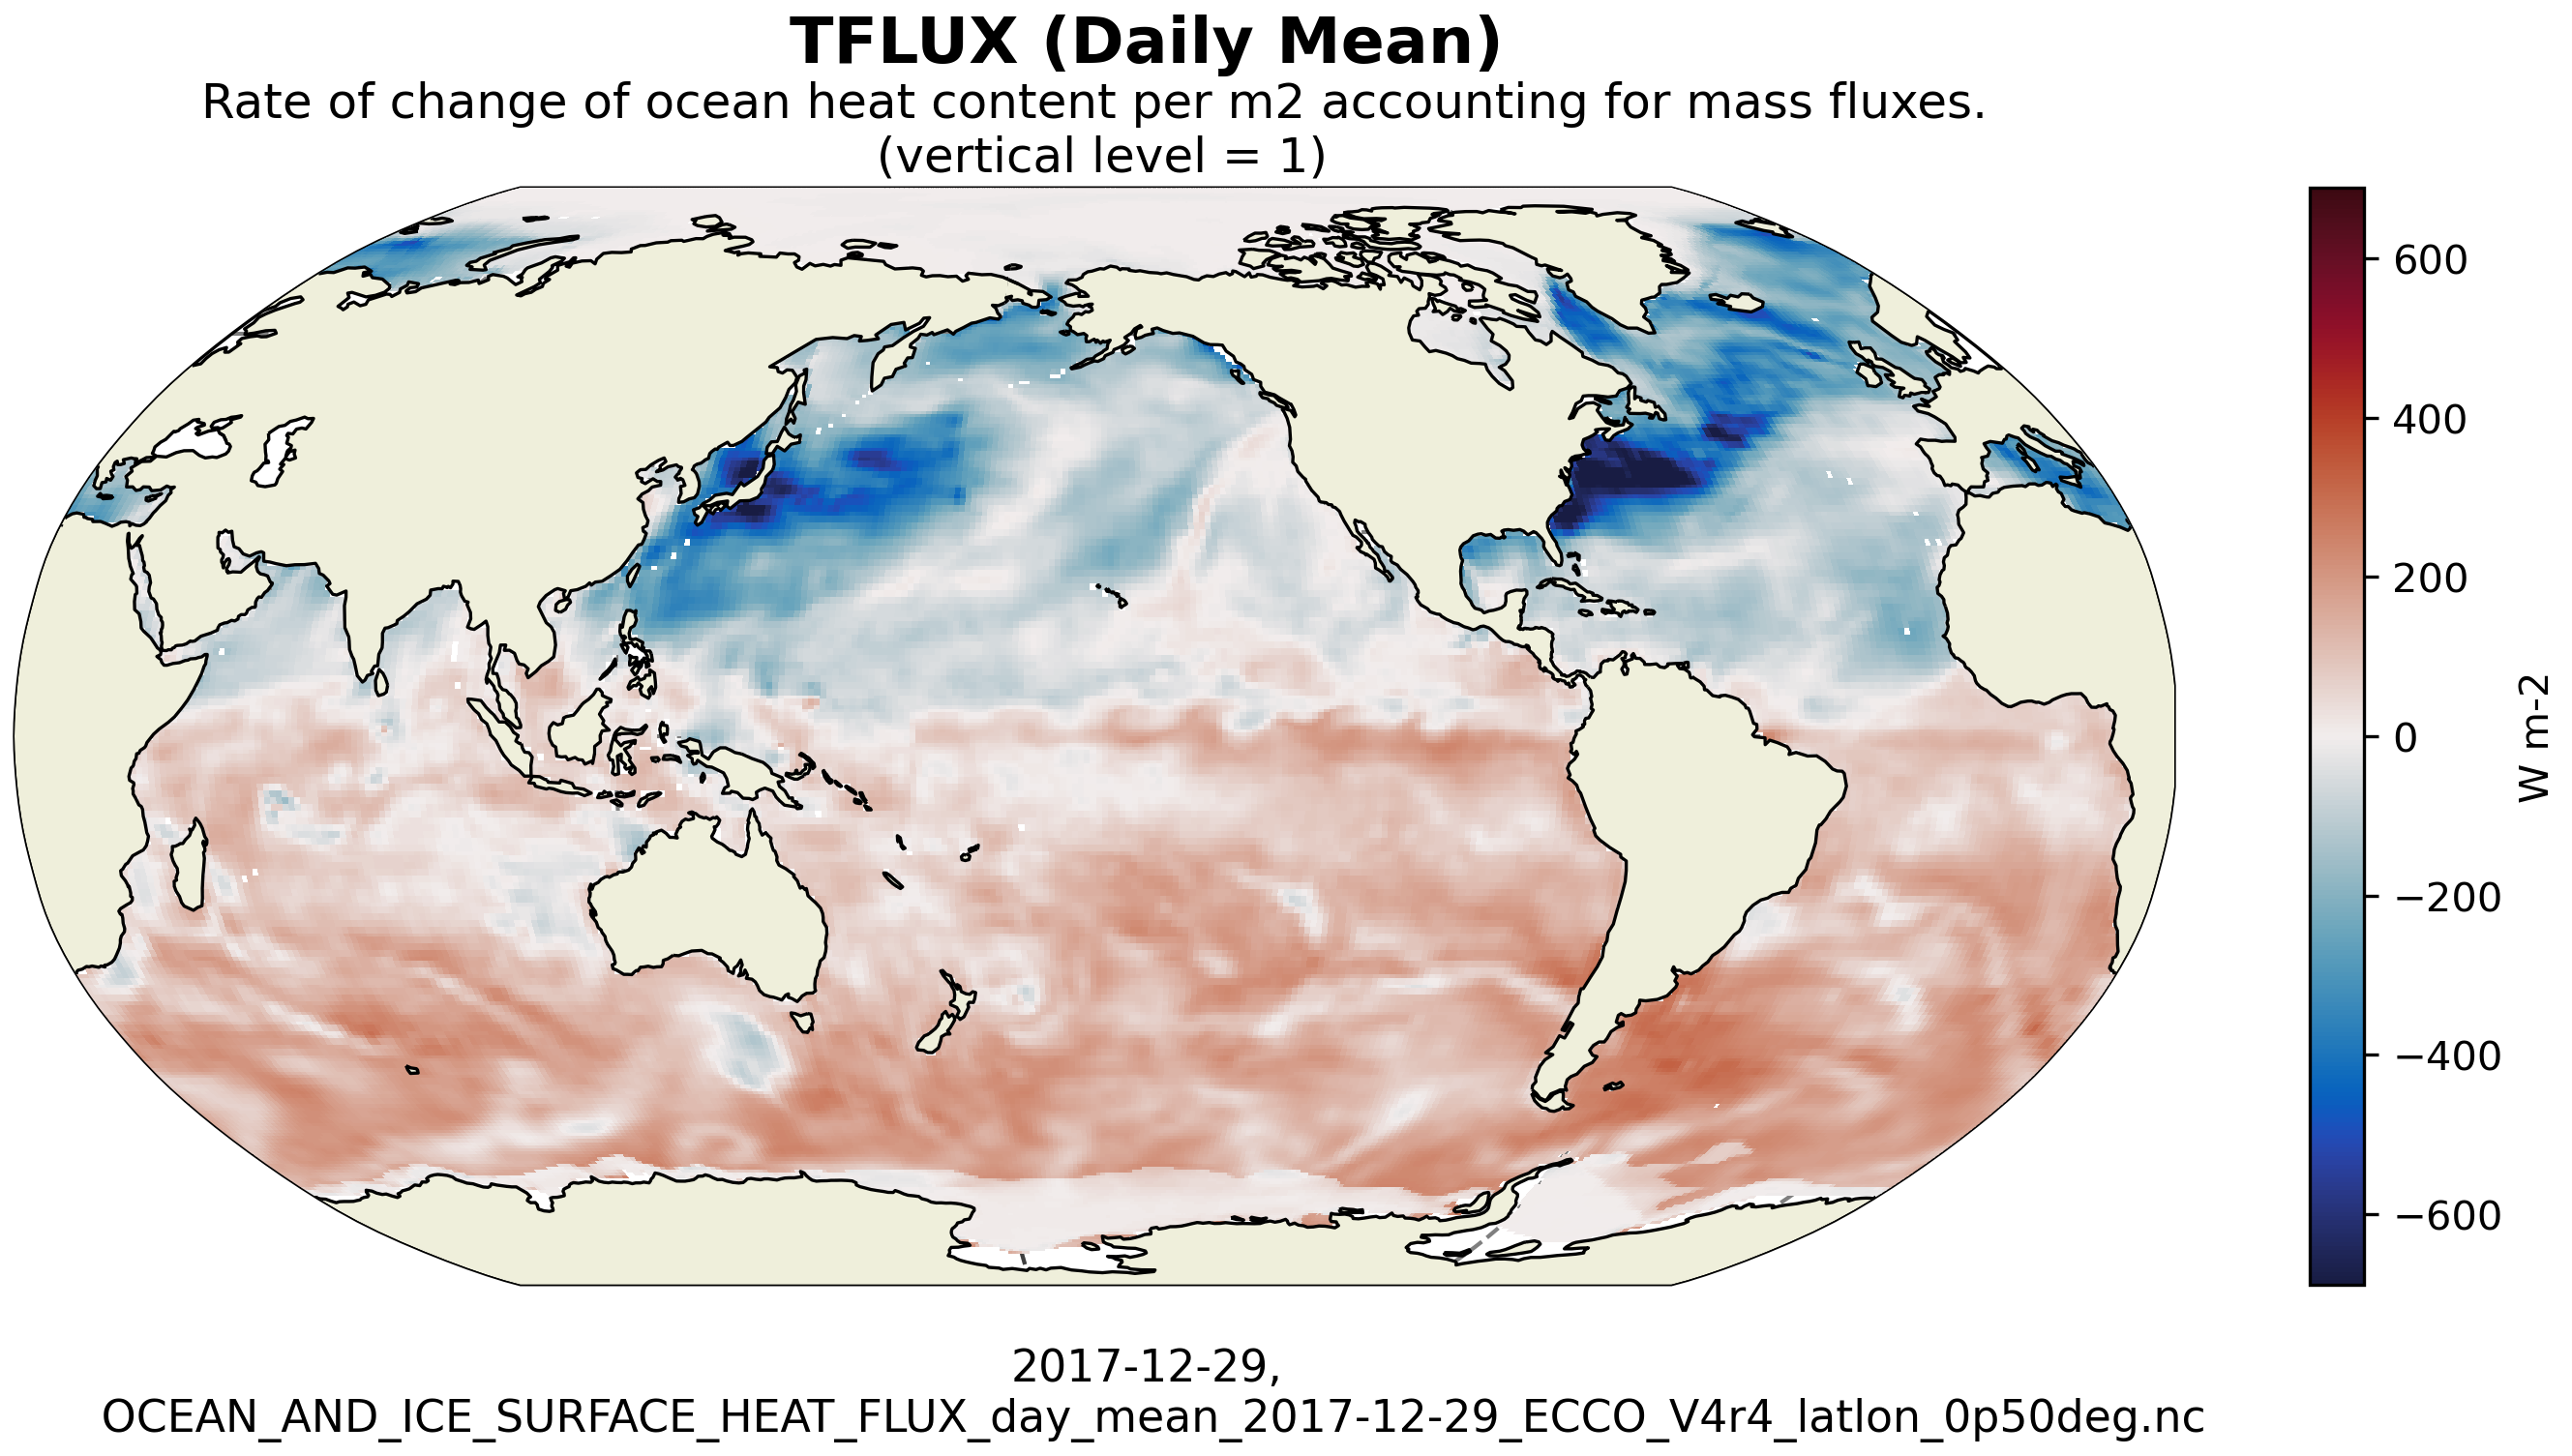
\includegraphics[scale=0.55]{../images/plots/v4r4/latlon_plots/Ocean_and_Sea-Ice_Surface_Heat_Fluxes/TFLUX.png}
\caption{Dataset: OCEAN\_AND\_ICE\_SURFACE\_HEAT\_FLUX, Variable: TFLUX}
\label{tab:table-OCEAN_AND_ICE_SURFACE_HEAT_FLUX_TFLUX-Plot}
\end{figure}
\newpage
\pagebreak
\subsubsection{Latlon Variable: oceQnet}
\begin{longtable}{|m{0.06\textwidth}|m{0.3\textwidth}|m{0.45\textwidth}|m{0.12\textwidth}|}
\caption{Attributes description of the variable 'oceQnet' from OCEAN\_AND\_ICE\_SURFACE\_HEAT\_FLUX's  dataset.}
\label{tab:table-OCEAN_AND_ICE_SURFACE_HEAT_FLUX_oceQnet} \\ 
\hline \endhead \hline \endfoot
\rowcolor{lightgray} \textbf{Storage Type} & \textbf{Variable Name} & \textbf{Description} & \textbf{Unit} \\ \hline
float32 & oceQnet & Net heat flux into the ocean surface & W m-2 \\ \hline
\multicolumn{4}{|c|}{\cellcolor{lightgray}{\textbf{Description of the variable in Common Data language (CDL)}}} \\ \hline
\multicolumn{4}{|c|}{\fontfamily{lmtt}\selectfont{\makecell{\parbox{.95\textwidth}{\vspace*{0.25cm} \footnotesize{float32 oceQnet(time, latitude, longitude)\\
\hspace*{0.5cm}oceQnet: \_FillValue = 9.96921e+36\\
\hspace*{0.5cm}oceQnet: coordinates = time\\
\hspace*{0.5cm}oceQnet: coverage\_content\_type = modelResult\\
\hspace*{0.5cm}oceQnet: direction = >0 increases potential temperature (THETA)\\
\hspace*{0.5cm}oceQnet: long\_name = Net heat flux into the ocean surface\\
\hspace*{0.5cm}oceQnet: standard\_name = surface downward heat flux in sea water\\
\hspace*{0.5cm}oceQnet: units = W m-2\\
\hspace*{0.5cm}oceQnet: valid\_max = 675.3716430664062\\
\hspace*{0.5cm}oceQnet: valid\_min = -1708.8460693359375\\
}}}}} \\ \hline
\rowcolor{lightgray} \multicolumn{4}{|c|}{\textbf{Comments}} \\ \hline
\multicolumn{4}{|p{1\textwidth}|}{\footnotesize{{Net heat flux into the ocean surface from all processes: air-sea turbulent and radiative fluxes and turbulent and conductive fluxes between the ocean and sea-ice and snow. note: oceqnet does not include the change in ocean heat content due to changing ocean ocean mass (ocefwflx). mass fluxes from evaporation, precipitation, and runoff (exfempmr) happen at the same temperature as the ocean surface temperature. consequently, empmr does not change ocean surface temperature. conversely, mass fluxes due to sea-ice thickening/thinning and snow melt in the model are assumed to happen at a fixed 0c. consequently, mass fluxes due to phase changes between seawater and sea-ice and snow induce a heat flux when the ocean surface temperaure is not 0c. the variable tflux does include the change in ocean heat content due to changing ocean mass.}}} \\ \hline
\end{longtable}

\begin{figure}[H]
\centering
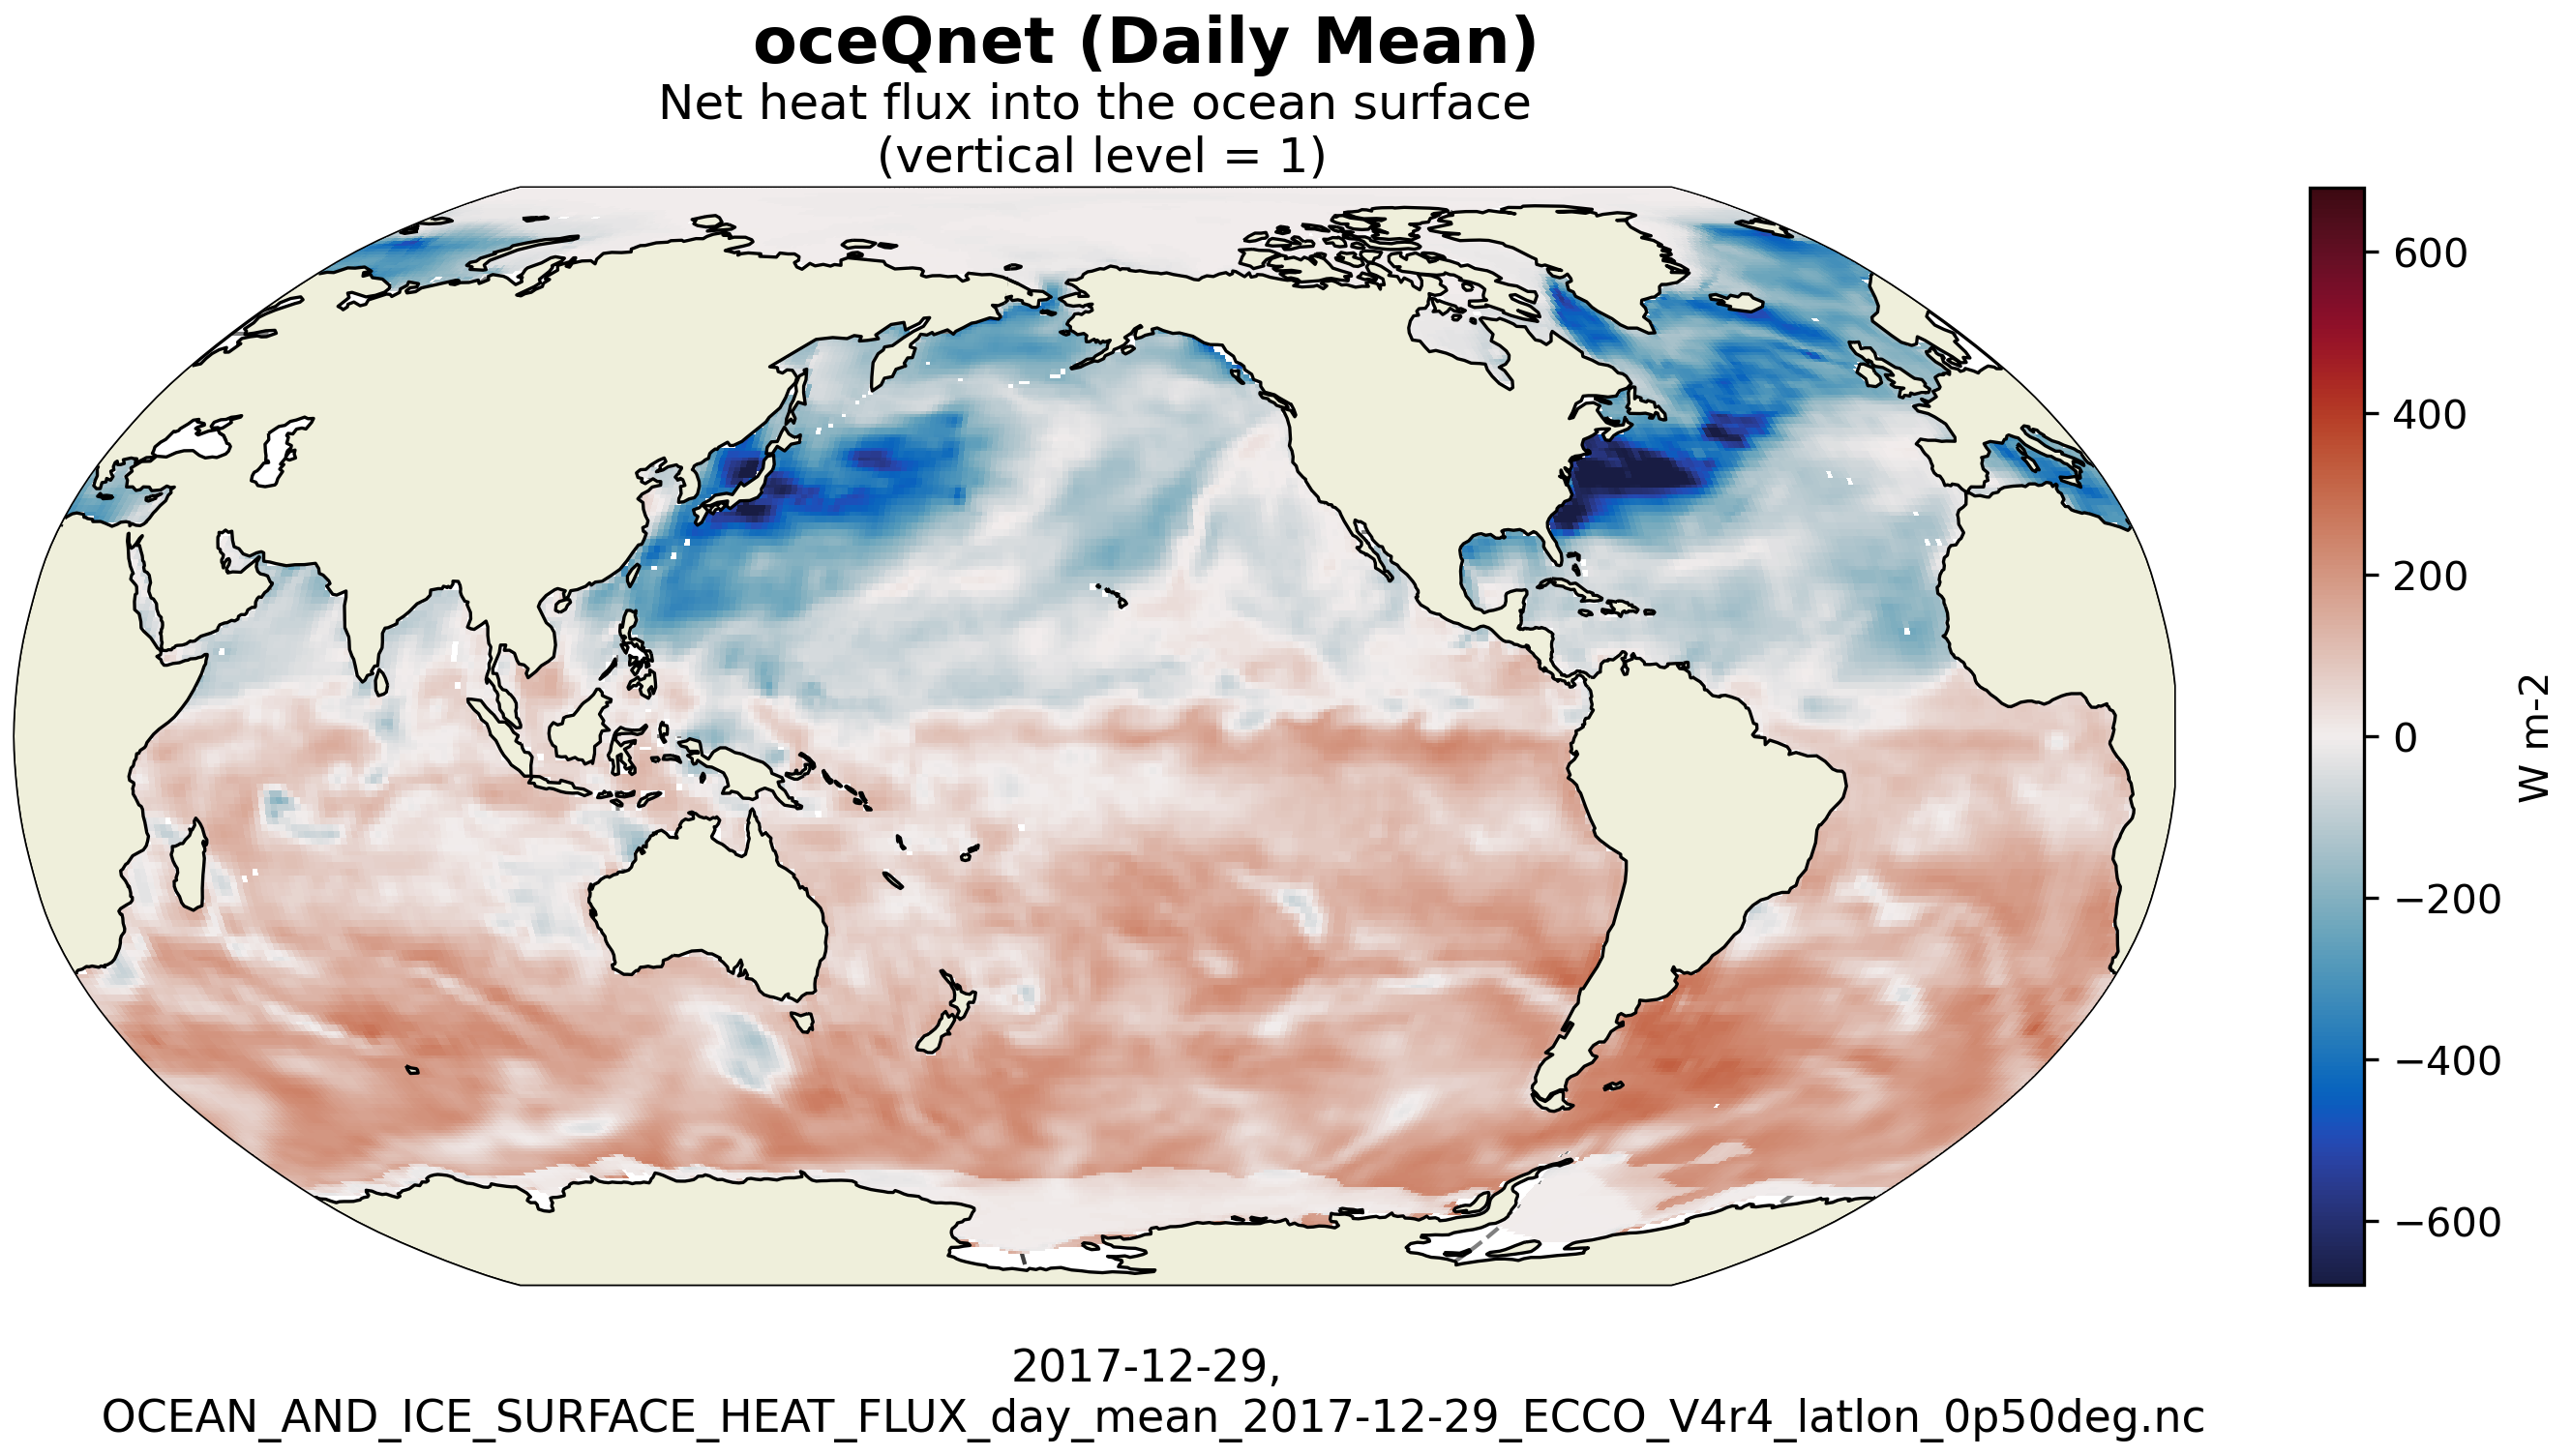
\includegraphics[scale=0.55]{../images/plots/v4r4/latlon_plots/Ocean_and_Sea-Ice_Surface_Heat_Fluxes/oceQnet.png}
\caption{Dataset: OCEAN\_AND\_ICE\_SURFACE\_HEAT\_FLUX, Variable: oceQnet}
\label{tab:table-OCEAN_AND_ICE_SURFACE_HEAT_FLUX_oceQnet-Plot}
\end{figure}
\newpage
\pagebreak
\subsubsection{Latlon Variable: oceQsw}
\begin{longtable}{|m{0.06\textwidth}|m{0.3\textwidth}|m{0.45\textwidth}|m{0.12\textwidth}|}
\caption{Attributes description of the variable 'oceQsw' from OCEAN\_AND\_ICE\_SURFACE\_HEAT\_FLUX's  dataset.}
\label{tab:table-OCEAN_AND_ICE_SURFACE_HEAT_FLUX_oceQsw} \\ 
\hline \endhead \hline \endfoot
\rowcolor{lightgray} \textbf{Storage Type} & \textbf{Variable Name} & \textbf{Description} & \textbf{Unit} \\ \hline
float32 & oceQsw & Net shortwave radiative flux across the ocean surface & W m-2 \\ \hline
\multicolumn{4}{|c|}{\cellcolor{lightgray}{\textbf{Description of the variable in Common Data language (CDL)}}} \\ \hline
\multicolumn{4}{|c|}{\fontfamily{lmtt}\selectfont{\makecell{\parbox{.95\textwidth}{\vspace*{0.25cm} \footnotesize{float32 oceQsw(time, latitude, longitude)\\
\hspace*{0.5cm}oceQsw: \_FillValue = 9.96921e+36\\
\hspace*{0.5cm}oceQsw: coordinates = time\\
\hspace*{0.5cm}oceQsw: coverage\_content\_type = modelResult\\
\hspace*{0.5cm}oceQsw: direction = >0 increases potential temperature (THETA)\\
\hspace*{0.5cm}oceQsw: long\_name = Net shortwave radiative flux across the ocean surface\\
\hspace*{0.5cm}oceQsw: units = W m-2\\
\hspace*{0.5cm}oceQsw: valid\_max = 655.6171264648438\\
\hspace*{0.5cm}oceQsw: valid\_min = -134.39808654785156\\
}}}}} \\ \hline
\rowcolor{lightgray} \multicolumn{4}{|c|}{\textbf{Comments}} \\ \hline
\multicolumn{4}{|p{1\textwidth}|}{\footnotesize{{Net shortwave radiative flux across the ocean surface. note: shortwave radiation penetrates below the surface grid cell.}}} \\ \hline
\end{longtable}

\begin{figure}[H]
\centering
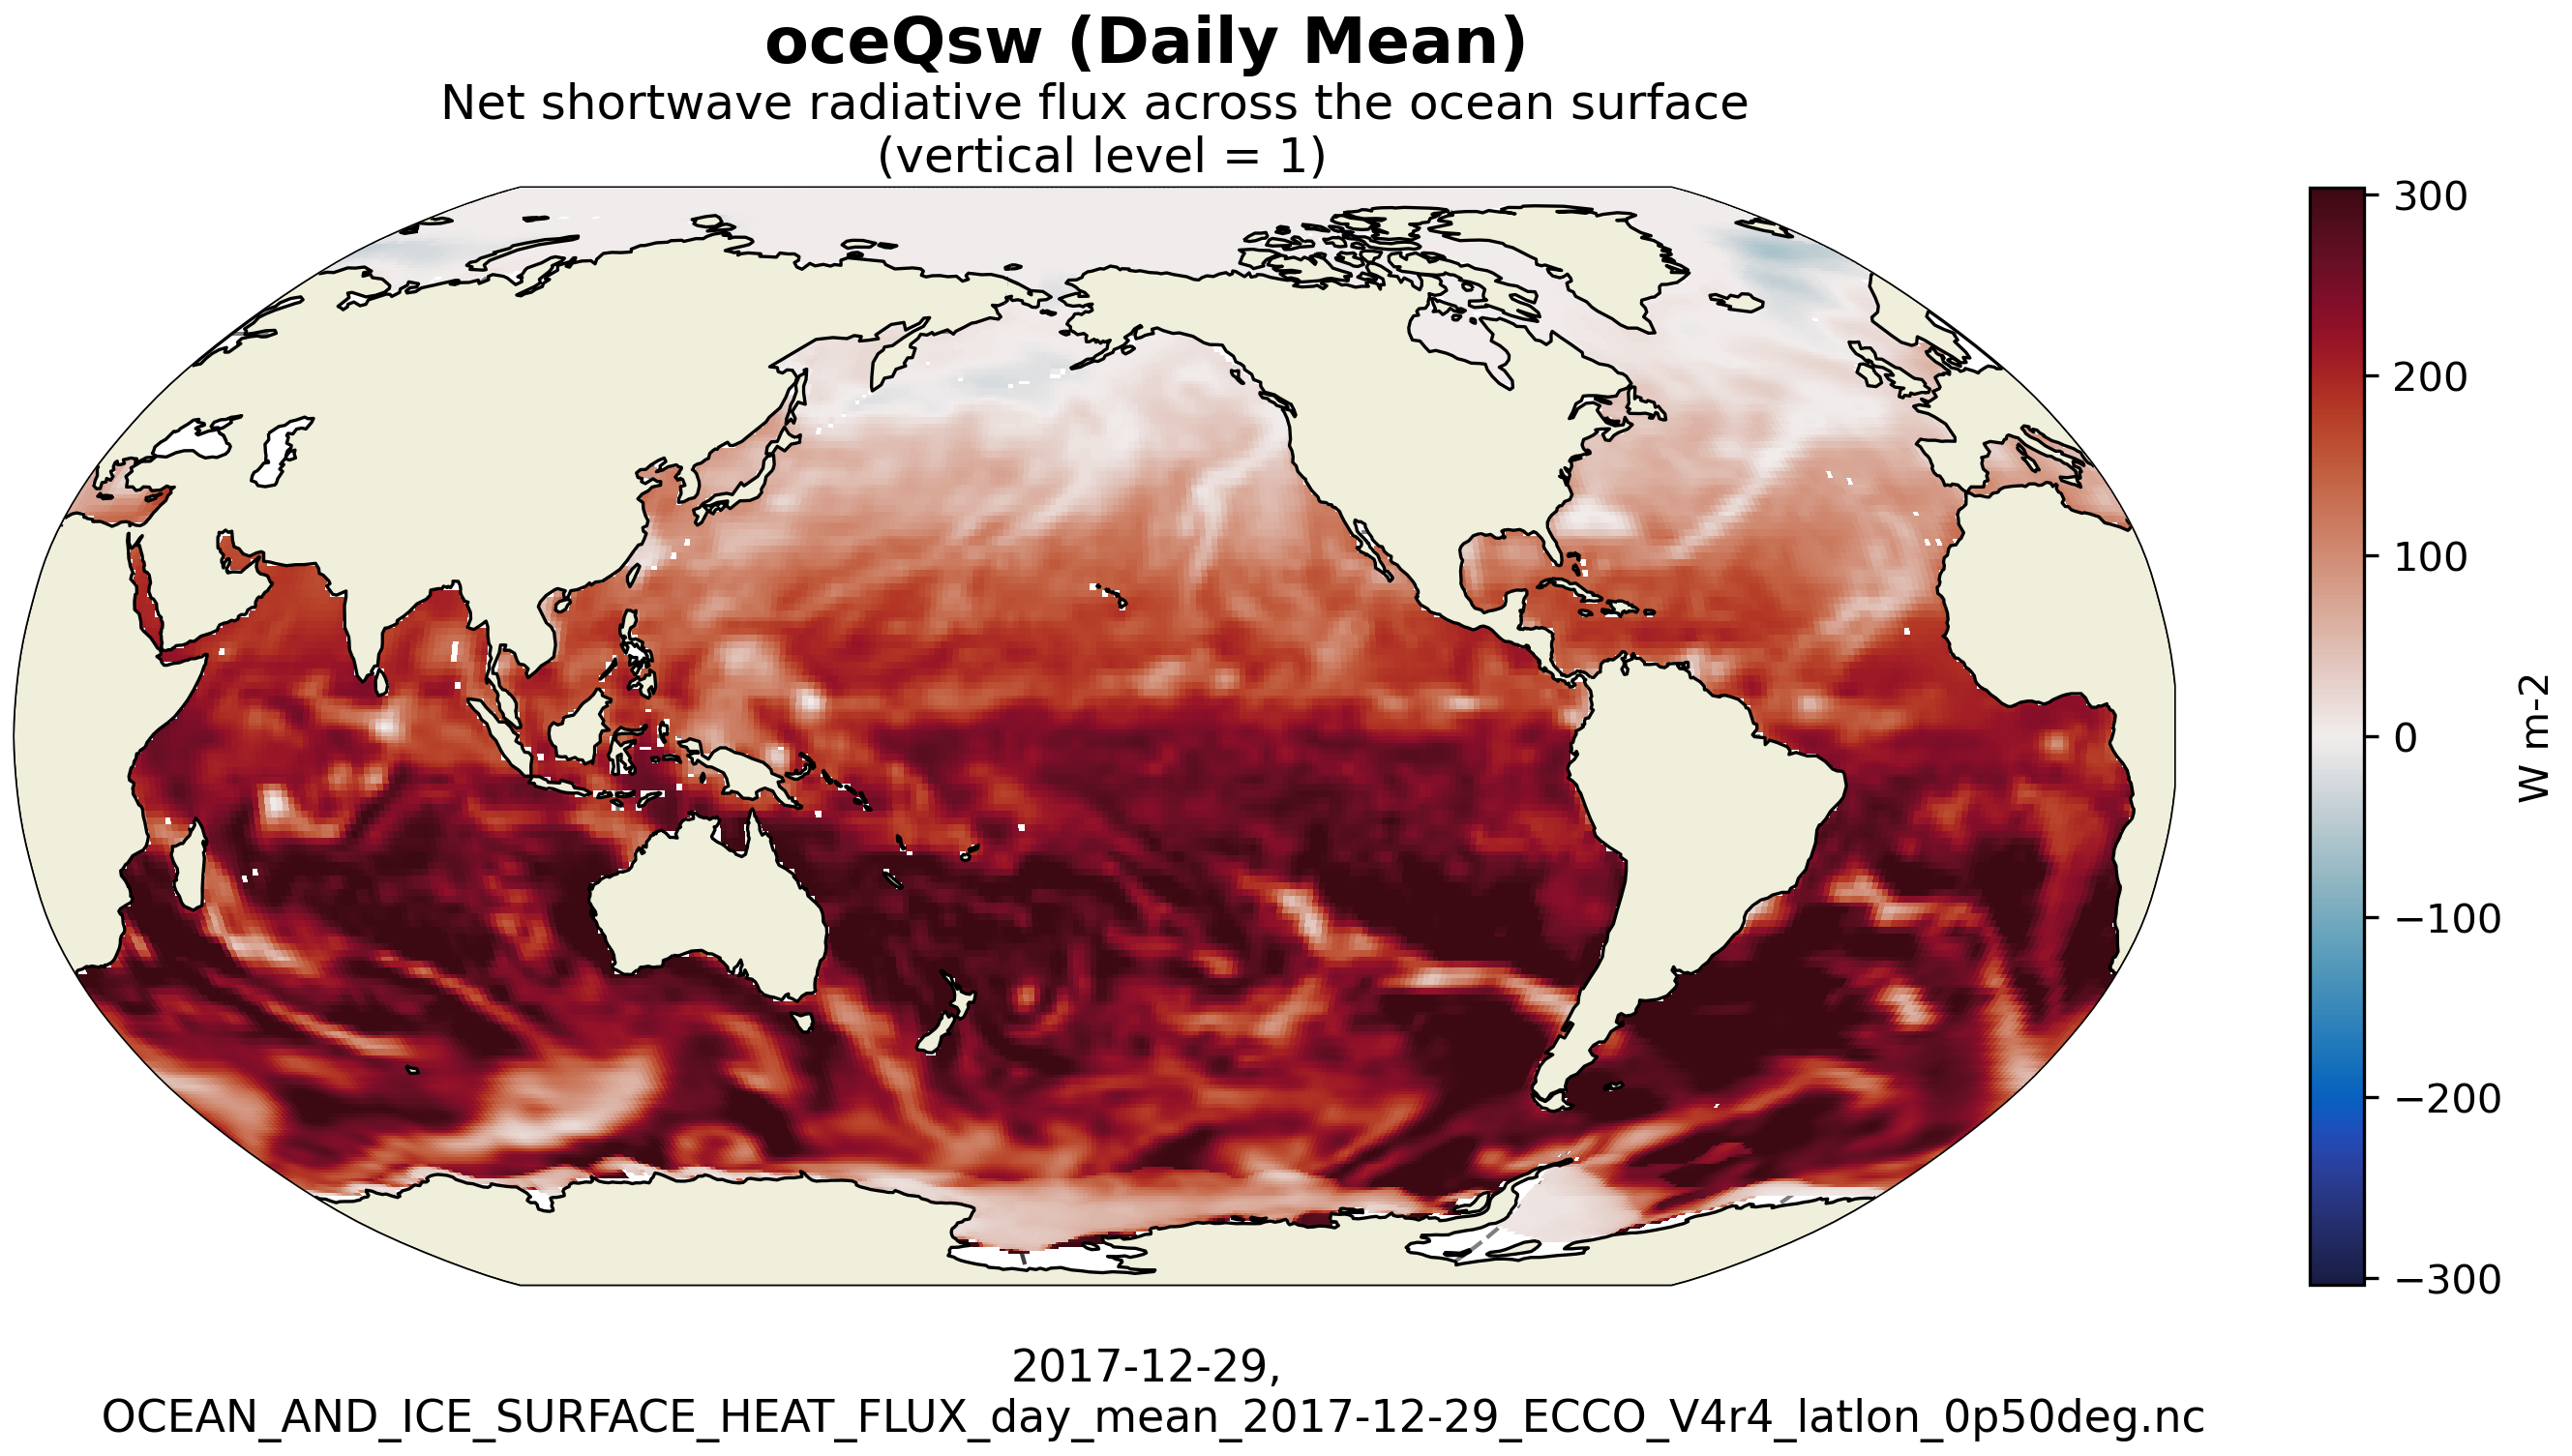
\includegraphics[scale=0.55]{../images/plots/v4r4/latlon_plots/Ocean_and_Sea-Ice_Surface_Heat_Fluxes/oceQsw.png}
\caption{Dataset: OCEAN\_AND\_ICE\_SURFACE\_HEAT\_FLUX, Variable: oceQsw}
\label{tab:table-OCEAN_AND_ICE_SURFACE_HEAT_FLUX_oceQsw-Plot}
\end{figure}
\newpage
\subsection{Latlon dataset of OCEAN\_AND\_ICE\_SURFACE\_STRESS}
\newp
\subsubsection{Overview}
This dataset provides 2D fields of ocean and sea-ice surface stress interpolated to a regular 0.5-degree grid from the ECCO Version 4 Release 4 (V4r4) ocean and sea-ice state estimate. The dataset is provided on daily-average and monthly-average time resolution. 
\begin{longtable}{|m{0.15\textwidth}|m{0.64\textwidth}|m{0.12\textwidth}|}
\caption{Coordinates and Variables in the dataset OCEAN\_AND\_ICE\_SURFACE\_STRESS}
\label{tab:table-OCEAN_AND_ICE_SURFACE_STRESS-fields} \\ 
\hline \endhead \hline \endfoot
\rowcolor{lightgray} \multicolumn{1}{|c|}{\textbf{Coordinates}} & \multicolumn{1}{|c|}{\textbf{Description of data coordinates}} &  \multicolumn{1}{|c|}{\textbf{Unit}}\\ \hline
time &Center time of averaging period &--none--  \\ \hline
latitude &Latitude at grid cell center &degrees\_north  \\ \hline
longitude &Longitude at grid cell center &degrees\_east  \\ \hline
time\_bnds &Time bounds of averaging period &--none--  \\ \hline
latitude\_bnds &Latitude bounds grid cells &--none--  \\ \hline
longitude\_bnds &Longitude bounds grid cells &--none--  \\ \hline
\rowcolor{lightgray} \multicolumn{1}{|c|}{\textbf{Variables}} & \multicolumn{1}{|c|}{\textbf{Description of data variables}} &  \multicolumn{1}{|c|}{\textbf{Unit}}\\ \hline
EXFtaue &Zonal (east-west) wind stress &N m-2  \\ \hline
EXFtaun &Meridional (north-south) wind stress &N m-2  \\ \hline
oceTAUE &Zonal (east-west) ocean surface stress &N m-2  \\ \hline
oceTAUN &Meridional (north-south) ocean surface stress &N m-2  \\ \hline
\end{longtable}

\newp
\pagebreak
\subsubsection{Latlon Variable: EXFtaue}
\begin{longtable}{|m{0.06\textwidth}|m{0.3\textwidth}|m{0.45\textwidth}|m{0.12\textwidth}|}
\caption{Attributes description of the variable 'EXFtaue' from OCEAN\_AND\_ICE\_SURFACE\_STRESS's  dataset.}
\label{tab:table-OCEAN_AND_ICE_SURFACE_STRESS_EXFtaue} \\ 
\hline \endhead \hline \endfoot
\rowcolor{lightgray} \textbf{Storage Type} & \textbf{Variable Name} & \textbf{Description} & \textbf{Unit} \\ \hline
float32 & EXFtaue & Zonal (east-west) wind stress & N m-2 \\ \hline
\multicolumn{4}{|c|}{\cellcolor{lightgray}{\textbf{Description of the variable in Common Data language (CDL)}}} \\ \hline
\multicolumn{4}{|c|}{\fontfamily{lmtt}\selectfont{\makecell{\parbox{.95\textwidth}{\vspace*{0.25cm} \footnotesize{float32 EXFtaue(time, latitude, longitude)\\
\hspace*{0.5cm}EXFtaue: \_FillValue = 9.96921e+36\\
\hspace*{0.5cm}EXFtaue: coordinates = time\\
\hspace*{0.5cm}EXFtaue: coverage\_content\_type = modelResult\\
\hspace*{0.5cm}EXFtaue: direction =  >0 increases eastward velocity (EVEL)\\
\hspace*{0.5cm}EXFtaue: long\_name = Zonal (east-west) wind stress\\
\hspace*{0.5cm}EXFtaue: standard\_name = surface downward eastward stress\\
\hspace*{0.5cm}EXFtaue: units = N m-2\\
\hspace*{0.5cm}EXFtaue: valid\_max = 3.284827709197998\\
\hspace*{0.5cm}EXFtaue: valid\_min = -3.1686902046203613\\
}}}}} \\ \hline
\rowcolor{lightgray} \multicolumn{4}{|c|}{\textbf{Comments}} \\ \hline
\multicolumn{4}{|p{1\textwidth}|}{\footnotesize{{Zonal (east-west) component of wind stress. note: exftaue is the zonal wind stress applied to the ocean and sea-ice. when sea-ice is present, the total zonal stress applied to the ocean surface is not exftaue, but a combination of the wind stress in the open water fraction (exftaue) and a stress from sea-ice in the ice-covered fraction (see ocetaue). exftaue is calculated by interpolating the model's x and y components of wind stress (exftaux and exftauy) to tracer cell centers and then finding the zonal component of the interpolated vectors. it is not recommended to use exftaue and exftaun for momentum budget calculations because interpolating exftaux and exftauy from the model grid to the lat-lon grid introduces errors. for momentum fluxes to the ocean surface see ocetaux and ocetauy.}}} \\ \hline
\end{longtable}

\begin{figure}[H]
\centering
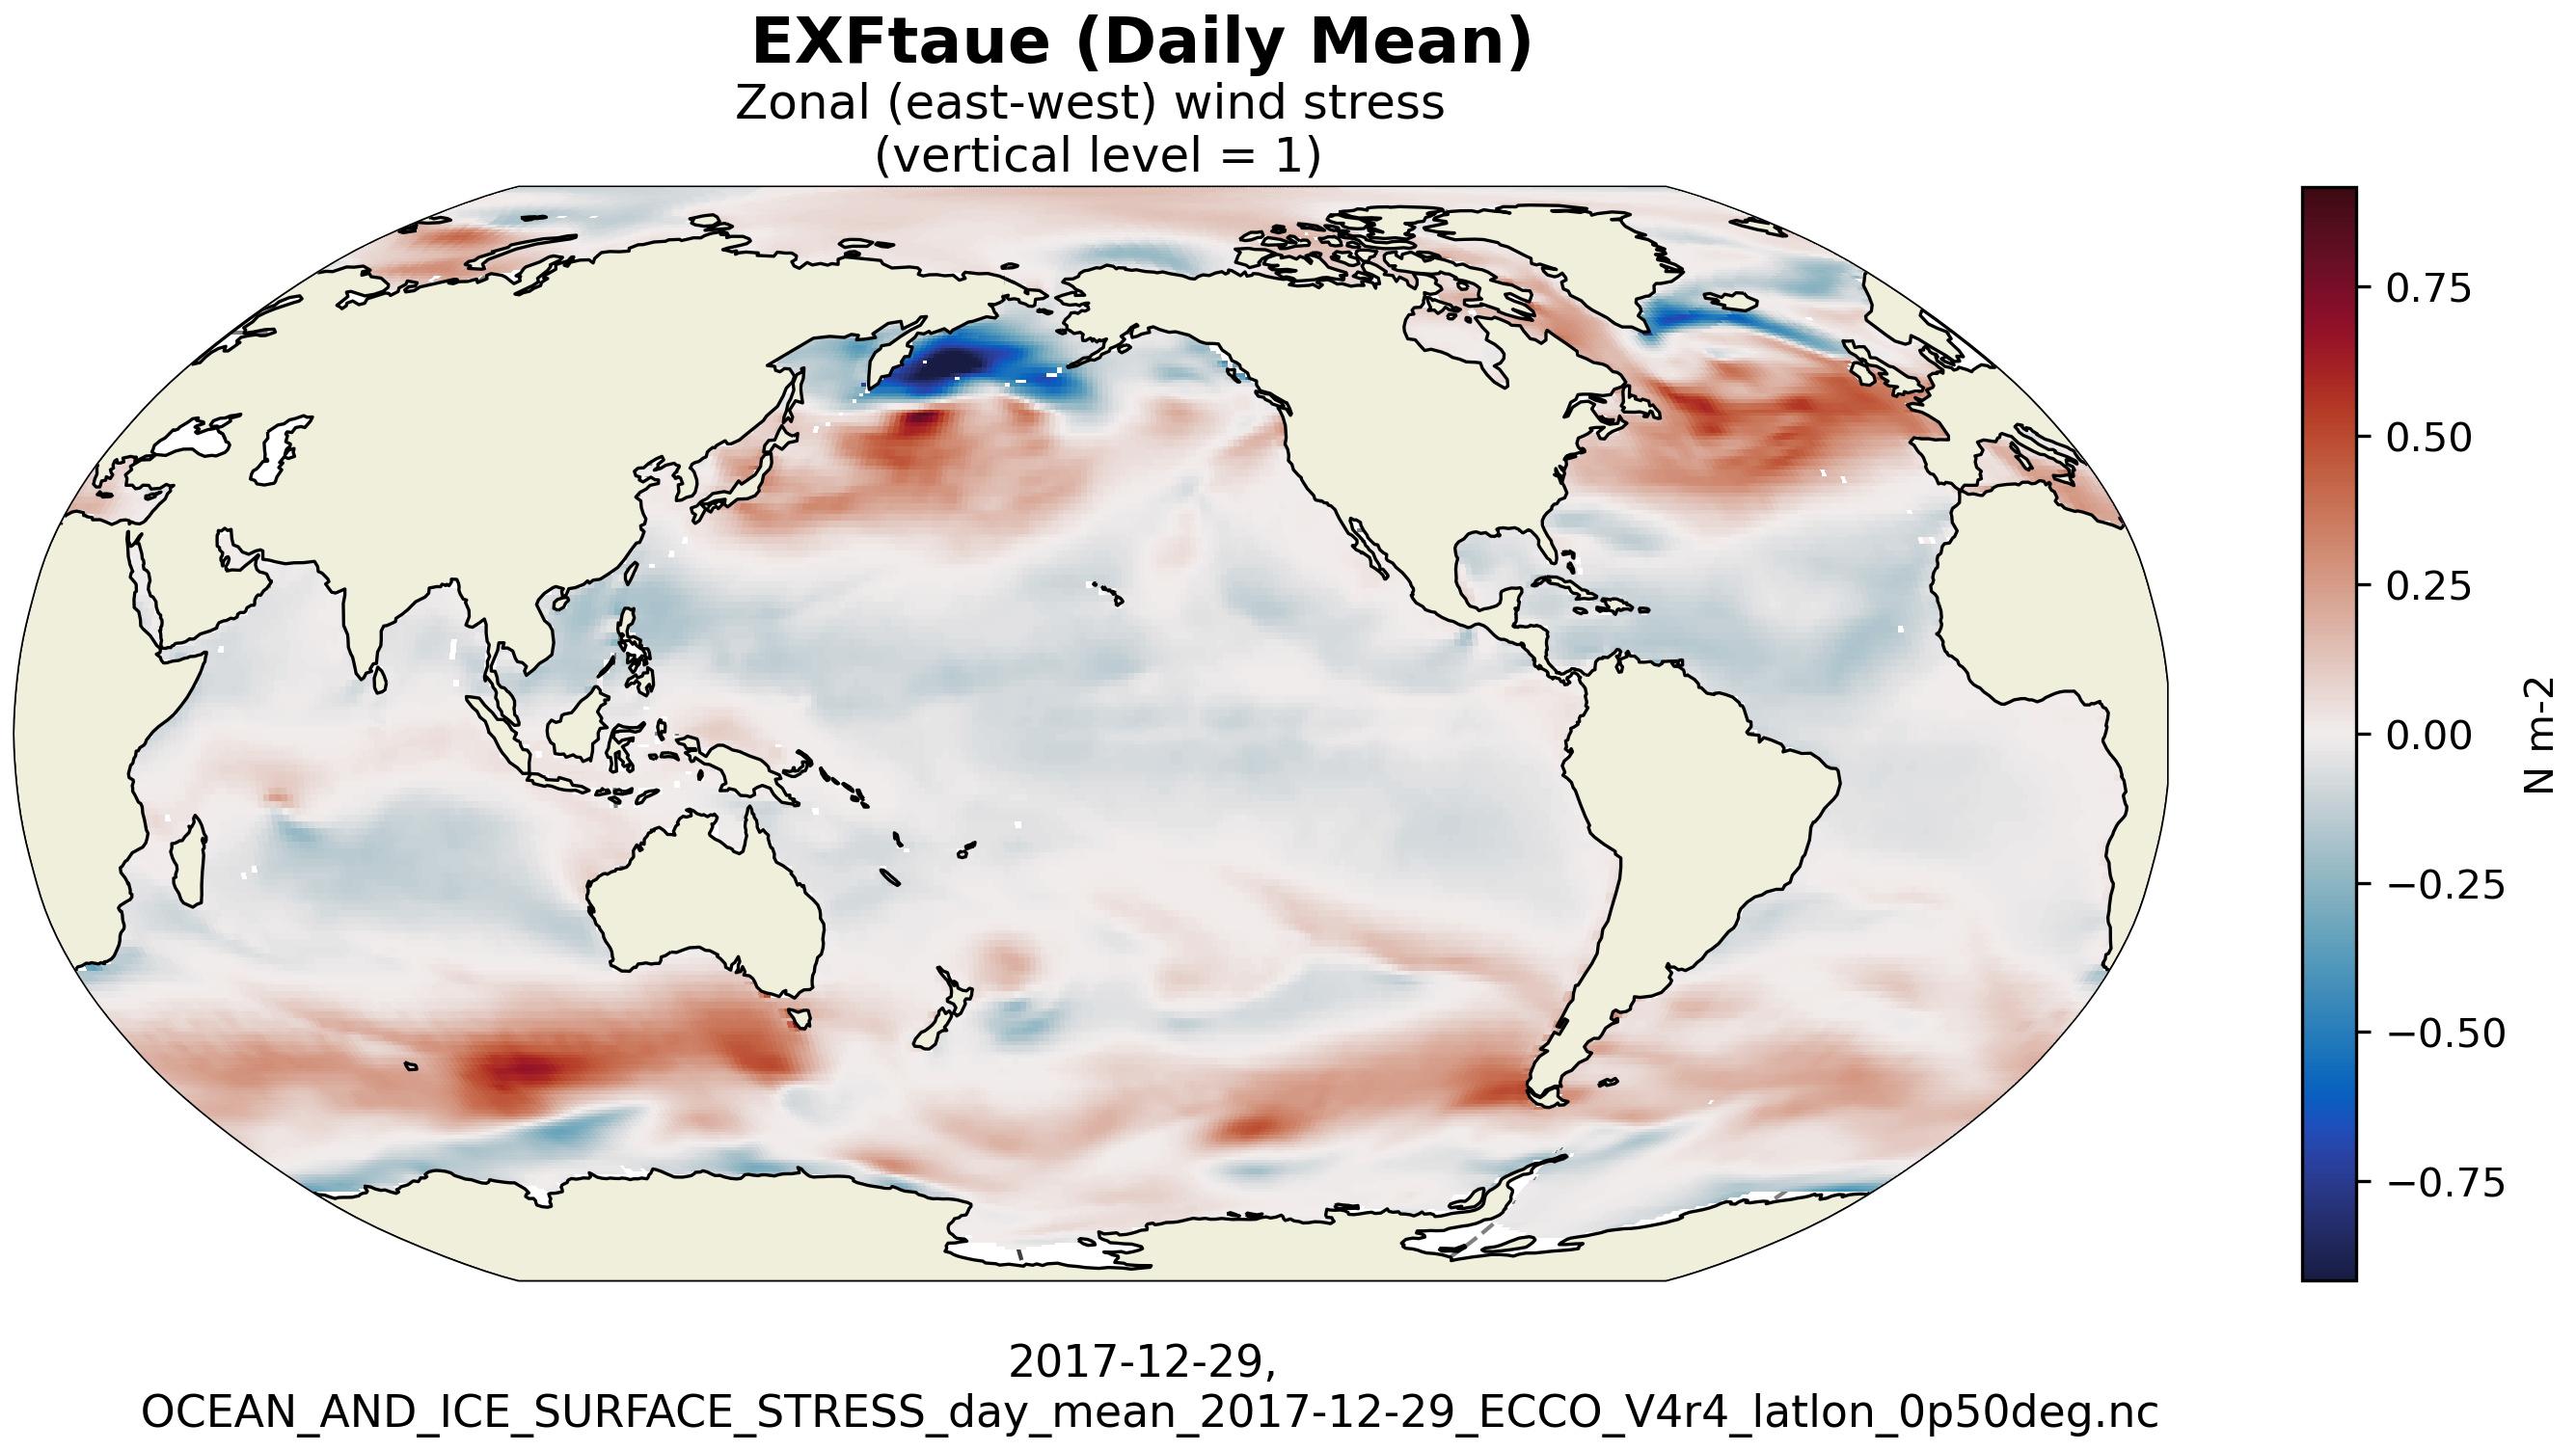
\includegraphics[scale=0.55]{../images/plots/v4r4/latlon_plots/Ocean_and_Sea-Ice_Surface_Stress/EXFtaue.png}
\caption{Dataset: OCEAN\_AND\_ICE\_SURFACE\_STRESS, Variable: EXFtaue}
\label{tab:table-OCEAN_AND_ICE_SURFACE_STRESS_EXFtaue-Plot}
\end{figure}
\newpage
\pagebreak
\subsubsection{Latlon Variable: EXFtaun}
\begin{longtable}{|m{0.06\textwidth}|m{0.3\textwidth}|m{0.45\textwidth}|m{0.12\textwidth}|}
\caption{Attributes description of the variable 'EXFtaun' from OCEAN\_AND\_ICE\_SURFACE\_STRESS's  dataset.}
\label{tab:table-OCEAN_AND_ICE_SURFACE_STRESS_EXFtaun} \\ 
\hline \endhead \hline \endfoot
\rowcolor{lightgray} \textbf{Storage Type} & \textbf{Variable Name} & \textbf{Description} & \textbf{Unit} \\ \hline
float32 & EXFtaun & Meridional (north-south) wind stress & N m-2 \\ \hline
\multicolumn{4}{|c|}{\cellcolor{lightgray}{\textbf{Description of the variable in Common Data language (CDL)}}} \\ \hline
\multicolumn{4}{|c|}{\fontfamily{lmtt}\selectfont{\makecell{\parbox{.95\textwidth}{\vspace*{0.25cm} \footnotesize{float32 EXFtaun(time, latitude, longitude)\\
\hspace*{0.5cm}EXFtaun: \_FillValue = 9.96921e+36\\
\hspace*{0.5cm}EXFtaun: coordinates = time\\
\hspace*{0.5cm}EXFtaun: coverage\_content\_type = modelResult\\
\hspace*{0.5cm}EXFtaun: direction =  >0 increases northward velocity (NVEL)\\
\hspace*{0.5cm}EXFtaun: long\_name = Meridional (north-south) wind stress\\
\hspace*{0.5cm}EXFtaun: standard\_name = surface downward northward stress\\
\hspace*{0.5cm}EXFtaun: units = N m-2\\
\hspace*{0.5cm}EXFtaun: valid\_max = 6.878159523010254\\
\hspace*{0.5cm}EXFtaun: valid\_min = -4.111213207244873\\
}}}}} \\ \hline
\rowcolor{lightgray} \multicolumn{4}{|c|}{\textbf{Comments}} \\ \hline
\multicolumn{4}{|p{1\textwidth}|}{\footnotesize{{Meridional (north-south) component of wind stress. note: exftaun is the stress applied to the ocean and sea-ice. when sea-ice is present, the total meridional stress applied to the ocean surface is not exftaun, but a combination of the wind stress in the open water fraction (exftaun) and a stress from sea-ice in the ice-covered fraction (see ocetaun).  exftaun is calculated by interpolating the model's x and y components of wind stress (exftaux and exftauy) to tracer cell centers and then determining the meridional component of the interpolated vectors. it is not recommended to use exftaue and exftaun for momentum budget calculations because interpolating exftaux and exftauy from the model grid to the lat-lon grid introduces errors. for momentum fluxes to the ocean surface see ocetaux and ocetauy.}}} \\ \hline
\end{longtable}

\begin{figure}[H]
\centering
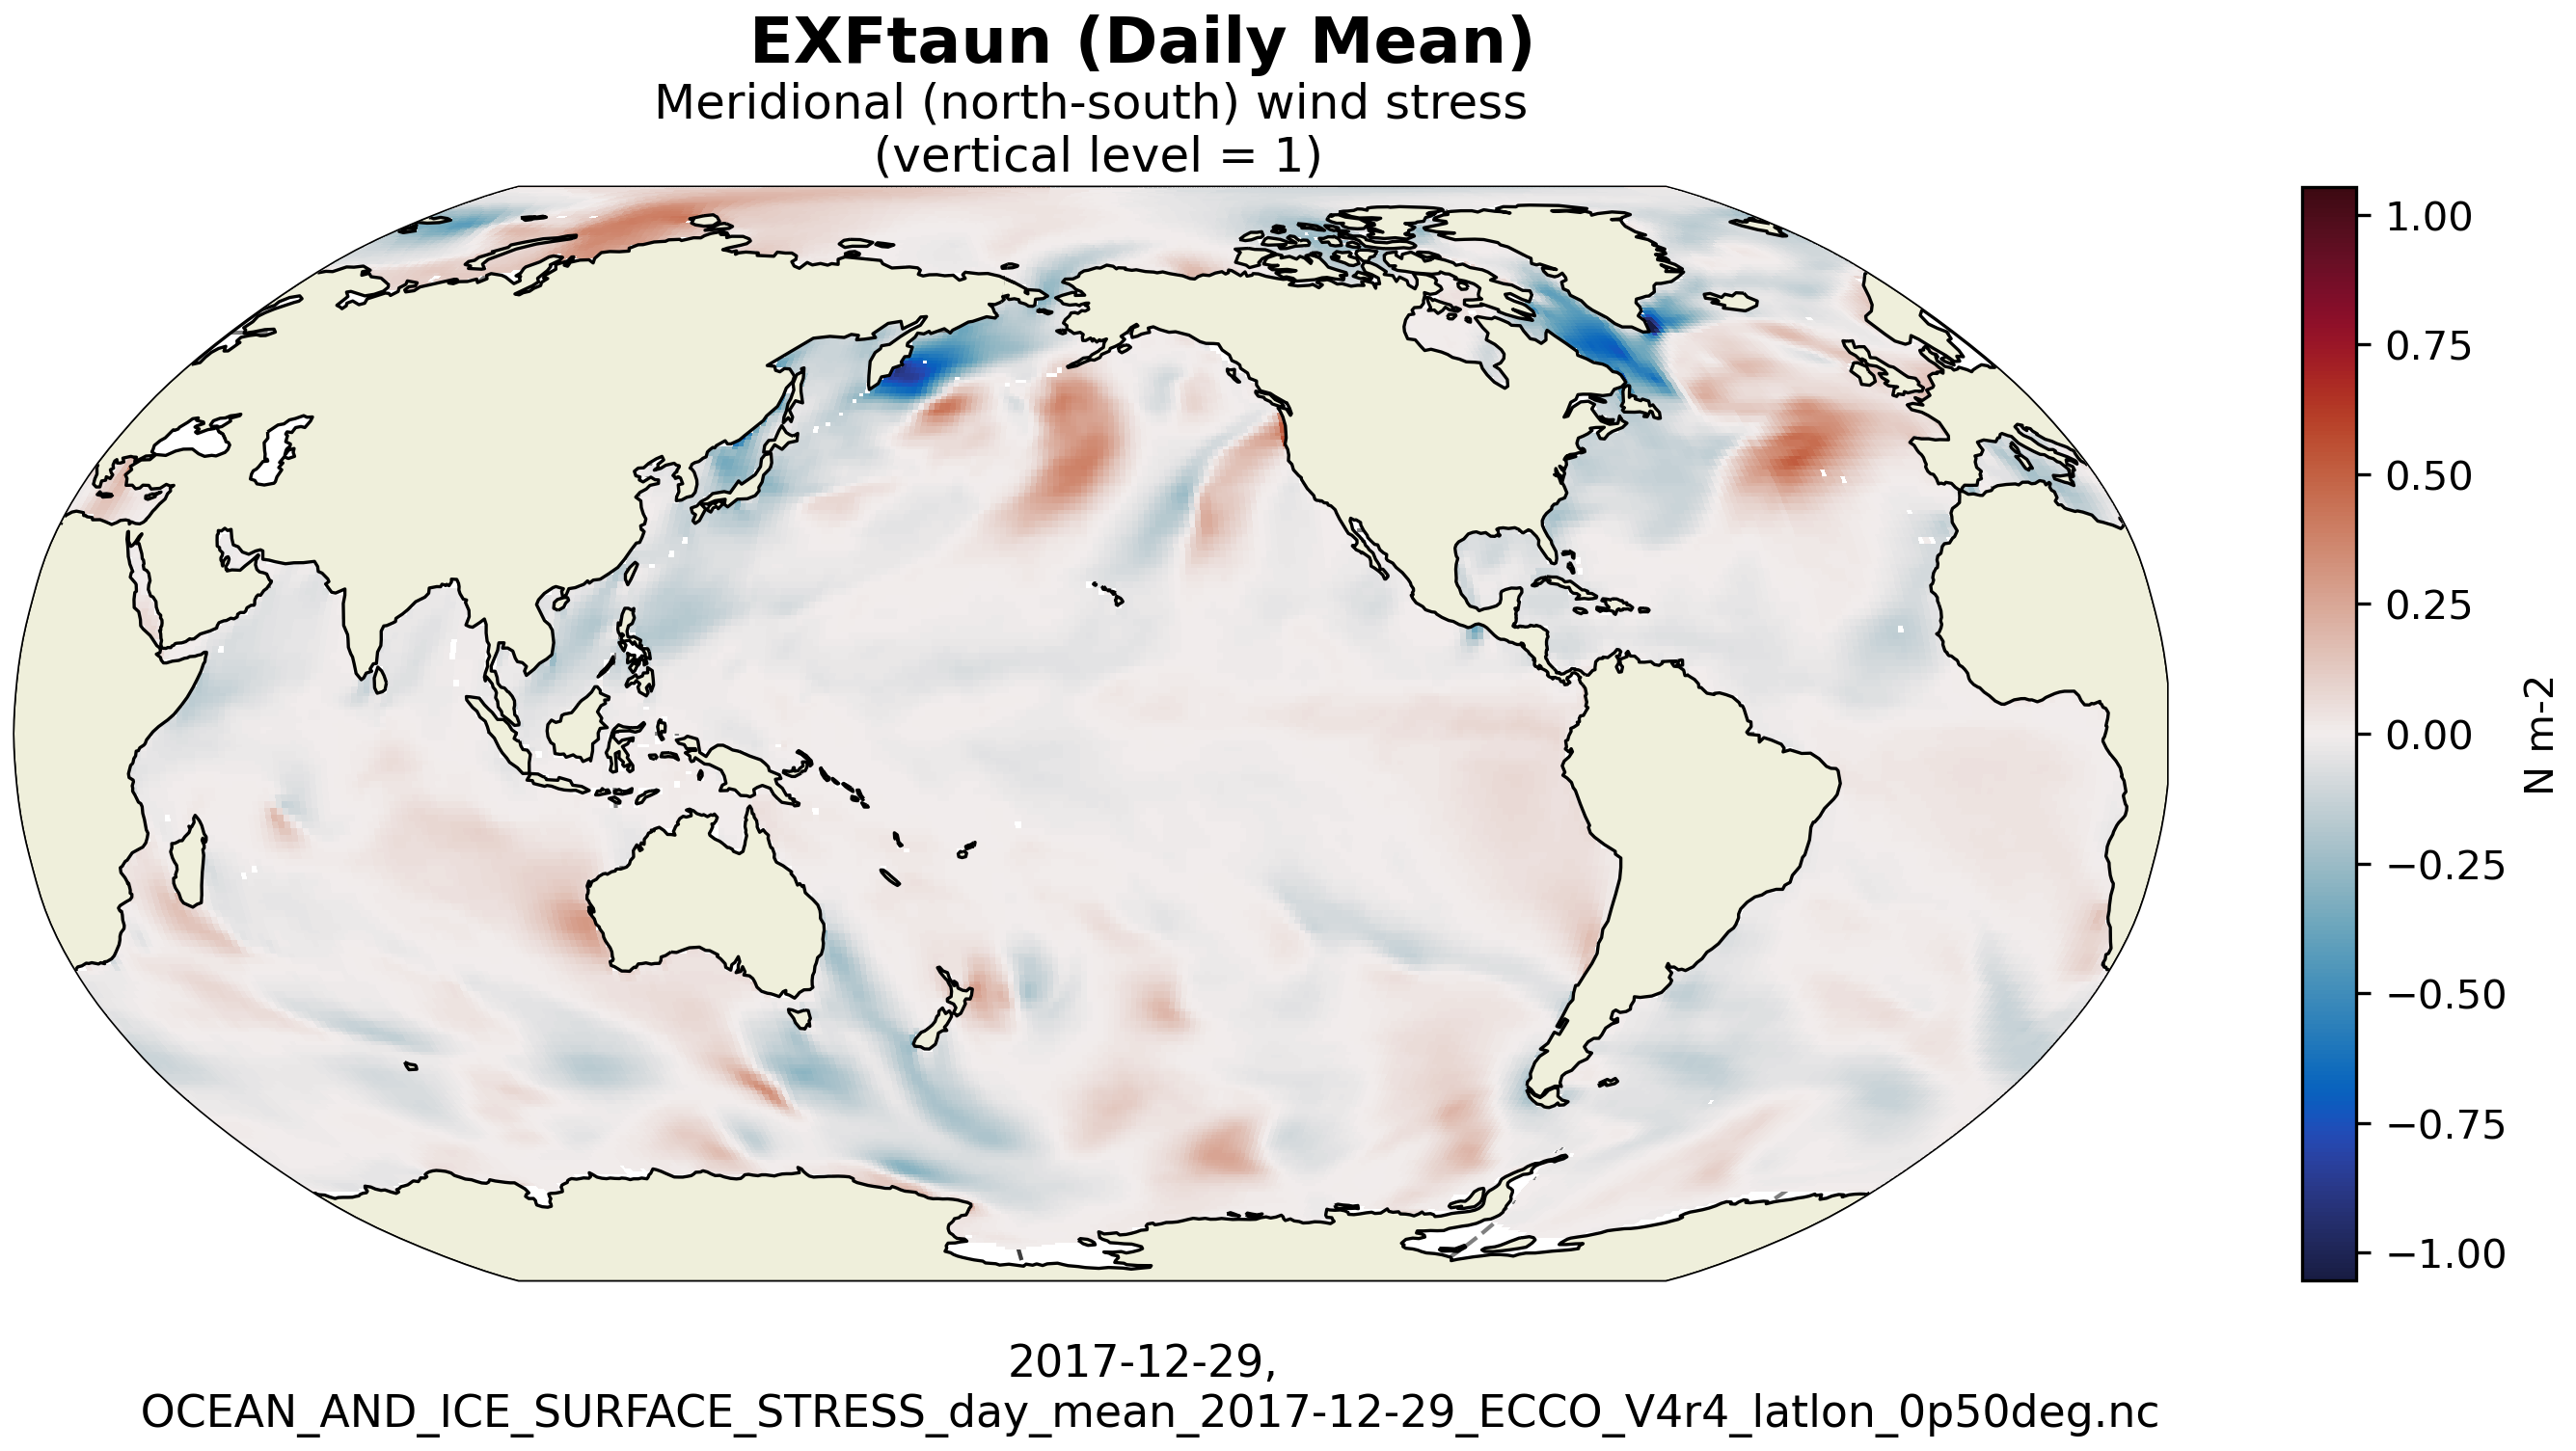
\includegraphics[scale=0.55]{../images/plots/v4r4/latlon_plots/Ocean_and_Sea-Ice_Surface_Stress/EXFtaun.png}
\caption{Dataset: OCEAN\_AND\_ICE\_SURFACE\_STRESS, Variable: EXFtaun}
\label{tab:table-OCEAN_AND_ICE_SURFACE_STRESS_EXFtaun-Plot}
\end{figure}
\newpage
\pagebreak
\subsubsection{Latlon Variable: oceTAUE}
\begin{longtable}{|m{0.06\textwidth}|m{0.3\textwidth}|m{0.45\textwidth}|m{0.12\textwidth}|}
\caption{Attributes description of the variable 'oceTAUE' from OCEAN\_AND\_ICE\_SURFACE\_STRESS's  dataset.}
\label{tab:table-OCEAN_AND_ICE_SURFACE_STRESS_oceTAUE} \\ 
\hline \endhead \hline \endfoot
\rowcolor{lightgray} \textbf{Storage Type} & \textbf{Variable Name} & \textbf{Description} & \textbf{Unit} \\ \hline
float32 & oceTAUE & Zonal (east-west) ocean surface stress & N m-2 \\ \hline
\multicolumn{4}{|c|}{\cellcolor{lightgray}{\textbf{Description of the variable in Common Data language (CDL)}}} \\ \hline
\multicolumn{4}{|c|}{\fontfamily{lmtt}\selectfont{\makecell{\parbox{.95\textwidth}{\vspace*{0.25cm} \footnotesize{float32 oceTAUE(time, latitude, longitude)\\
\hspace*{0.5cm}oceTAUE: \_FillValue = 9.96921e+36\\
\hspace*{0.5cm}oceTAUE: coordinates = time\\
\hspace*{0.5cm}oceTAUE: coverage\_content\_type = modelResult\\
\hspace*{0.5cm}oceTAUE: direction =  >0 increases eastward velocity (EVEL)\\
\hspace*{0.5cm}oceTAUE: long\_name = Zonal (east-west) ocean surface stress\\
\hspace*{0.5cm}oceTAUE: standard\_name = surface downward eastward stress\\
\hspace*{0.5cm}oceTAUE: units = N m-2\\
\hspace*{0.5cm}oceTAUE: valid\_max = 2.000103712081909\\
\hspace*{0.5cm}oceTAUE: valid\_min = -2.058817148208618\\
}}}}} \\ \hline
\rowcolor{lightgray} \multicolumn{4}{|c|}{\textbf{Comments}} \\ \hline
\multicolumn{4}{|p{1\textwidth}|}{\footnotesize{{Zonal (east-west) component of ocean surface stress due to wind and sea-ice. note: ocetaue is calculated by interpolating the model's x and y components of ocean surface stress (ocetaux and ocetauy) to tracer cell centers and then finding the zonal component of the interpolated vectors.}}} \\ \hline
\end{longtable}

\begin{figure}[H]
\centering
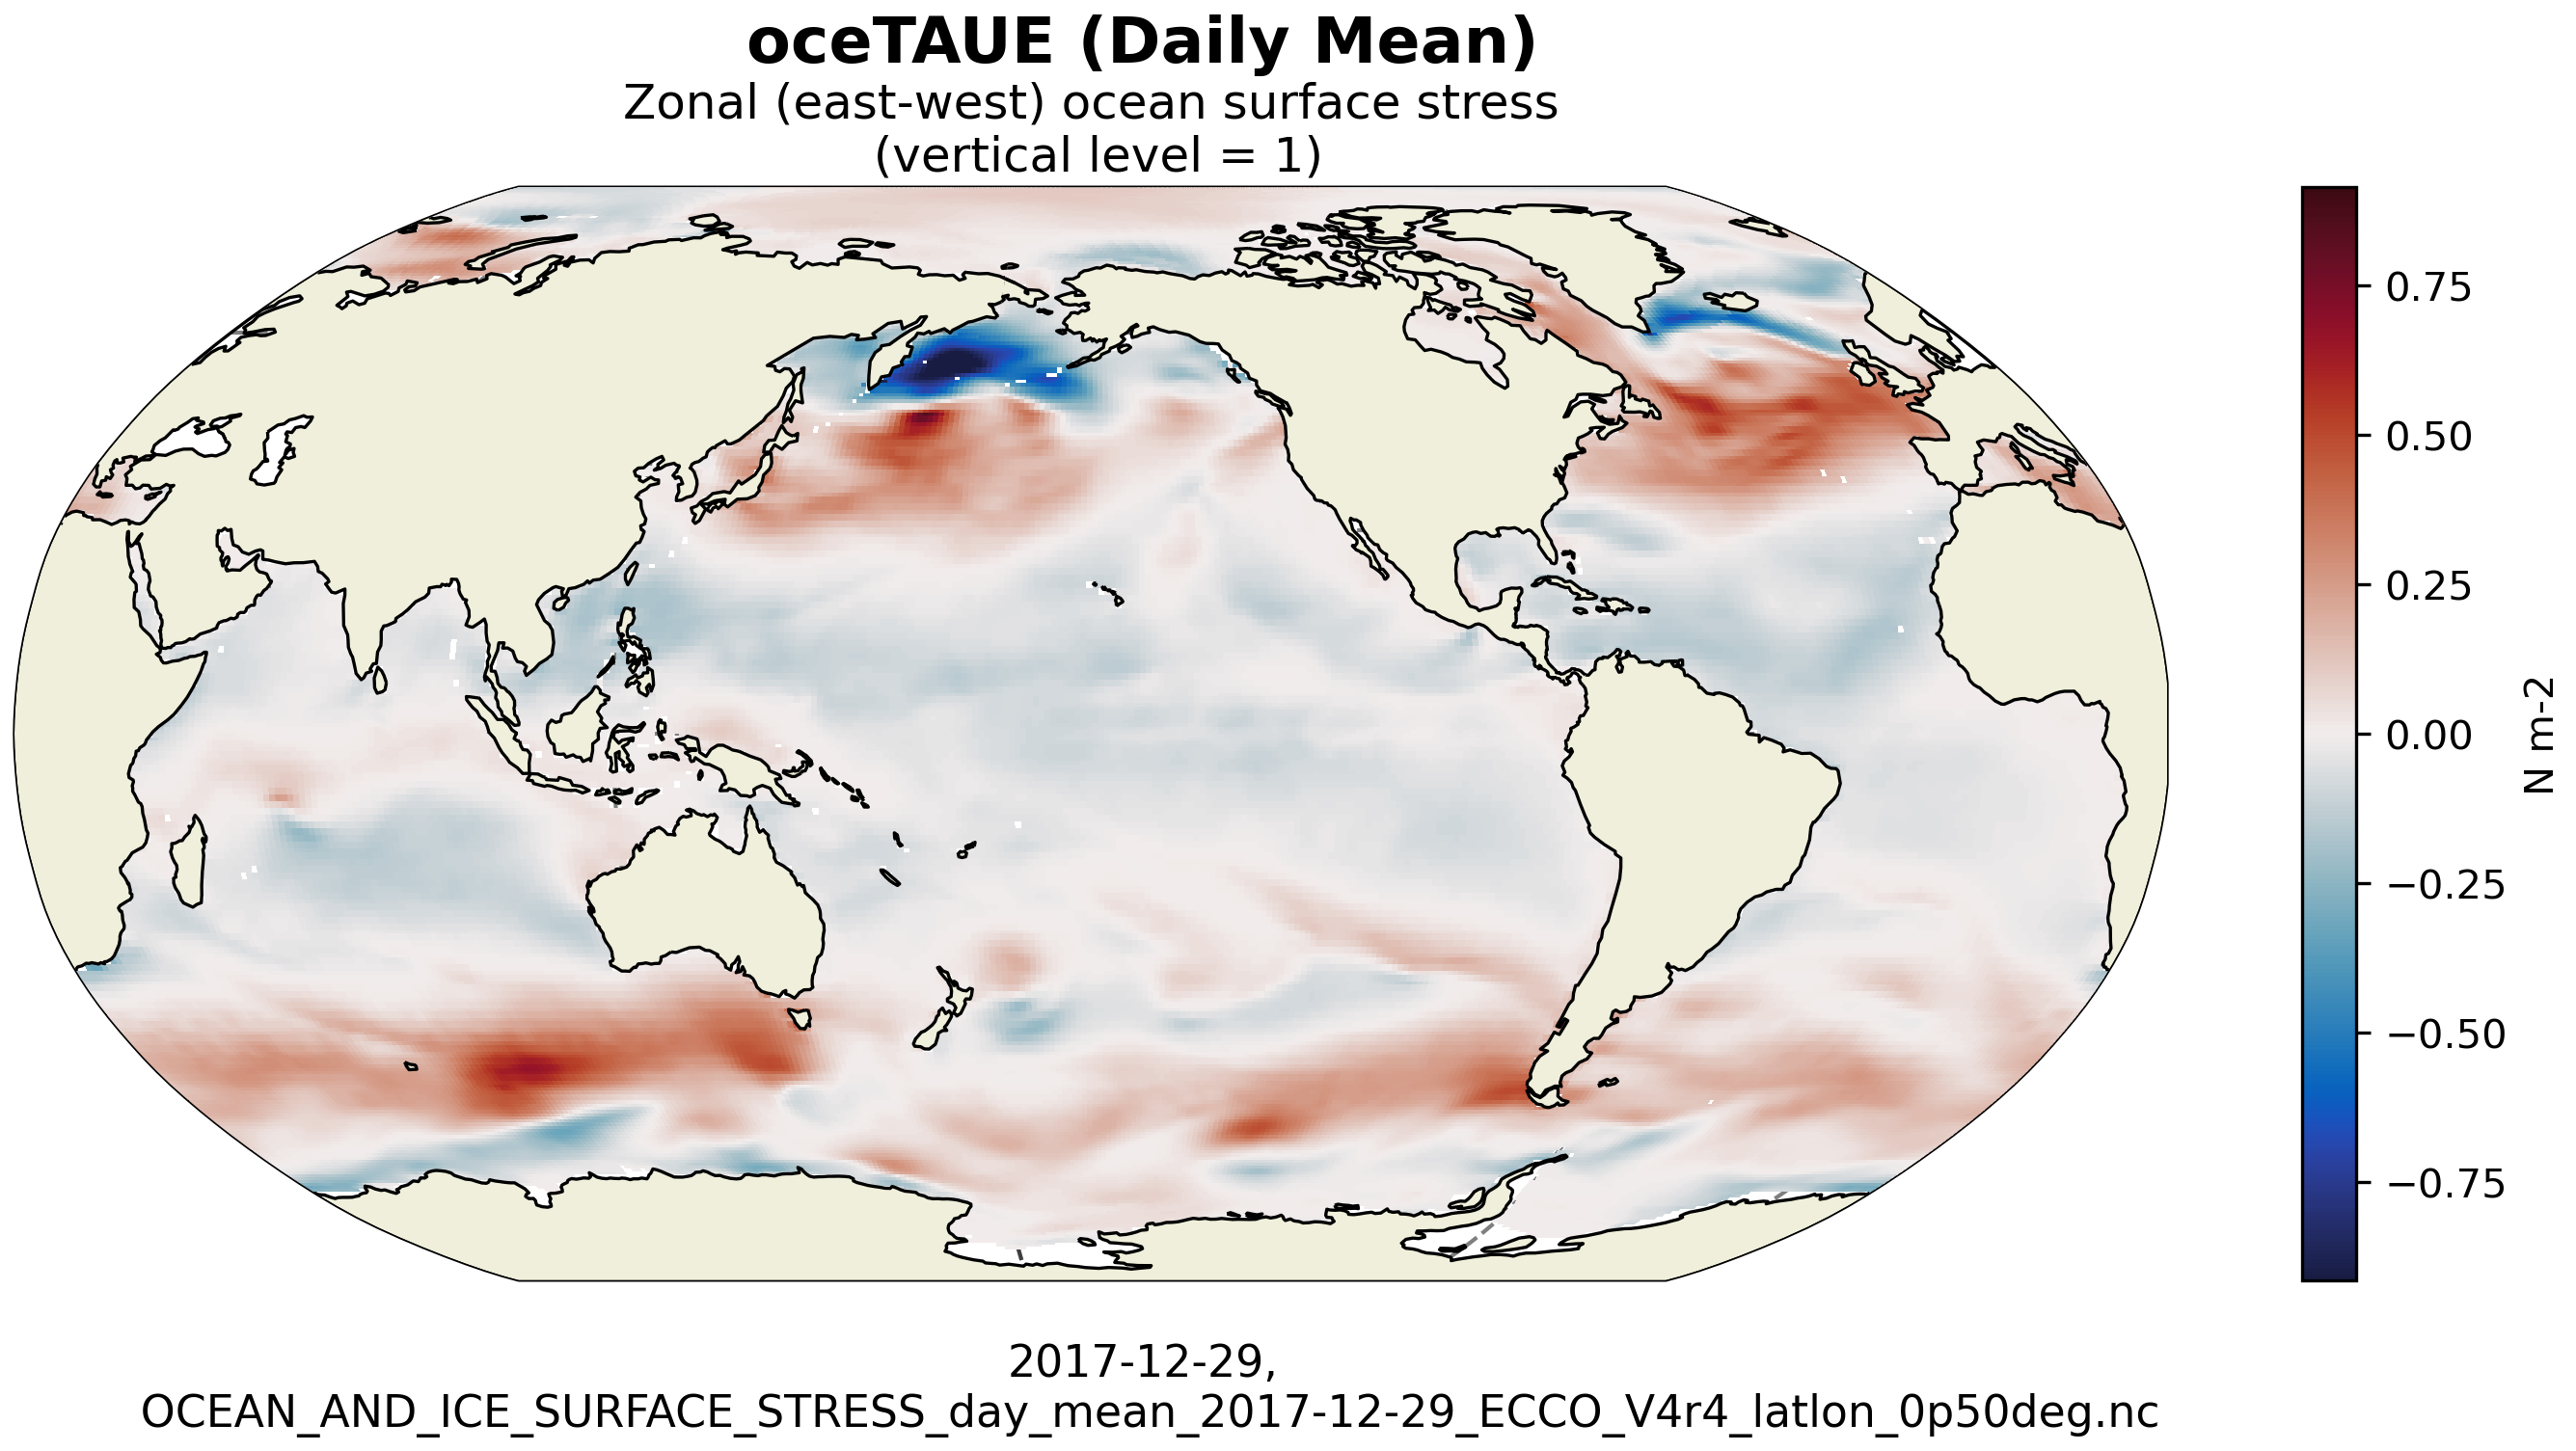
\includegraphics[scale=0.55]{../images/plots/v4r4/latlon_plots/Ocean_and_Sea-Ice_Surface_Stress/oceTAUE.png}
\caption{Dataset: OCEAN\_AND\_ICE\_SURFACE\_STRESS, Variable: oceTAUE}
\label{tab:table-OCEAN_AND_ICE_SURFACE_STRESS_oceTAUE-Plot}
\end{figure}
\newpage
\pagebreak
\subsubsection{Latlon Variable: oceTAUN}
\begin{longtable}{|m{0.06\textwidth}|m{0.3\textwidth}|m{0.45\textwidth}|m{0.12\textwidth}|}
\caption{Attributes description of the variable 'oceTAUN' from OCEAN\_AND\_ICE\_SURFACE\_STRESS's  dataset.}
\label{tab:table-OCEAN_AND_ICE_SURFACE_STRESS_oceTAUN} \\ 
\hline \endhead \hline \endfoot
\rowcolor{lightgray} \textbf{Storage Type} & \textbf{Variable Name} & \textbf{Description} & \textbf{Unit} \\ \hline
float32 & oceTAUN & Meridional (north-south) ocean surface stress & N m-2 \\ \hline
\multicolumn{4}{|c|}{\cellcolor{lightgray}{\textbf{Description of the variable in Common Data language (CDL)}}} \\ \hline
\multicolumn{4}{|c|}{\fontfamily{lmtt}\selectfont{\makecell{\parbox{.95\textwidth}{\vspace*{0.25cm} \footnotesize{float32 oceTAUN(time, latitude, longitude)\\
\hspace*{0.5cm}oceTAUN: \_FillValue = 9.96921e+36\\
\hspace*{0.5cm}oceTAUN: coordinates = time\\
\hspace*{0.5cm}oceTAUN: coverage\_content\_type = modelResult\\
\hspace*{0.5cm}oceTAUN: direction =  >0 increases northward velocity (NVEL)\\
\hspace*{0.5cm}oceTAUN: long\_name = Meridional (north-south) ocean surface stress\\
\hspace*{0.5cm}oceTAUN: standard\_name = surface downward northward stress\\
\hspace*{0.5cm}oceTAUN: units = N m-2\\
\hspace*{0.5cm}oceTAUN: valid\_max = 2.019313097000122\\
\hspace*{0.5cm}oceTAUN: valid\_min = -2.4036266803741455\\
}}}}} \\ \hline
\rowcolor{lightgray} \multicolumn{4}{|c|}{\textbf{Comments}} \\ \hline
\multicolumn{4}{|p{1\textwidth}|}{\footnotesize{{Meridional (north-south) component of ocean surface stress due to wind and sea-ice. note: ocetaun is calculated by interpolating the model's x and y components of ocean surface stress (ocetaux and ocetauy) to tracer cell centers and then finding the meridional component of the interpolated vectors.}}} \\ \hline
\end{longtable}

\begin{figure}[H]
\centering
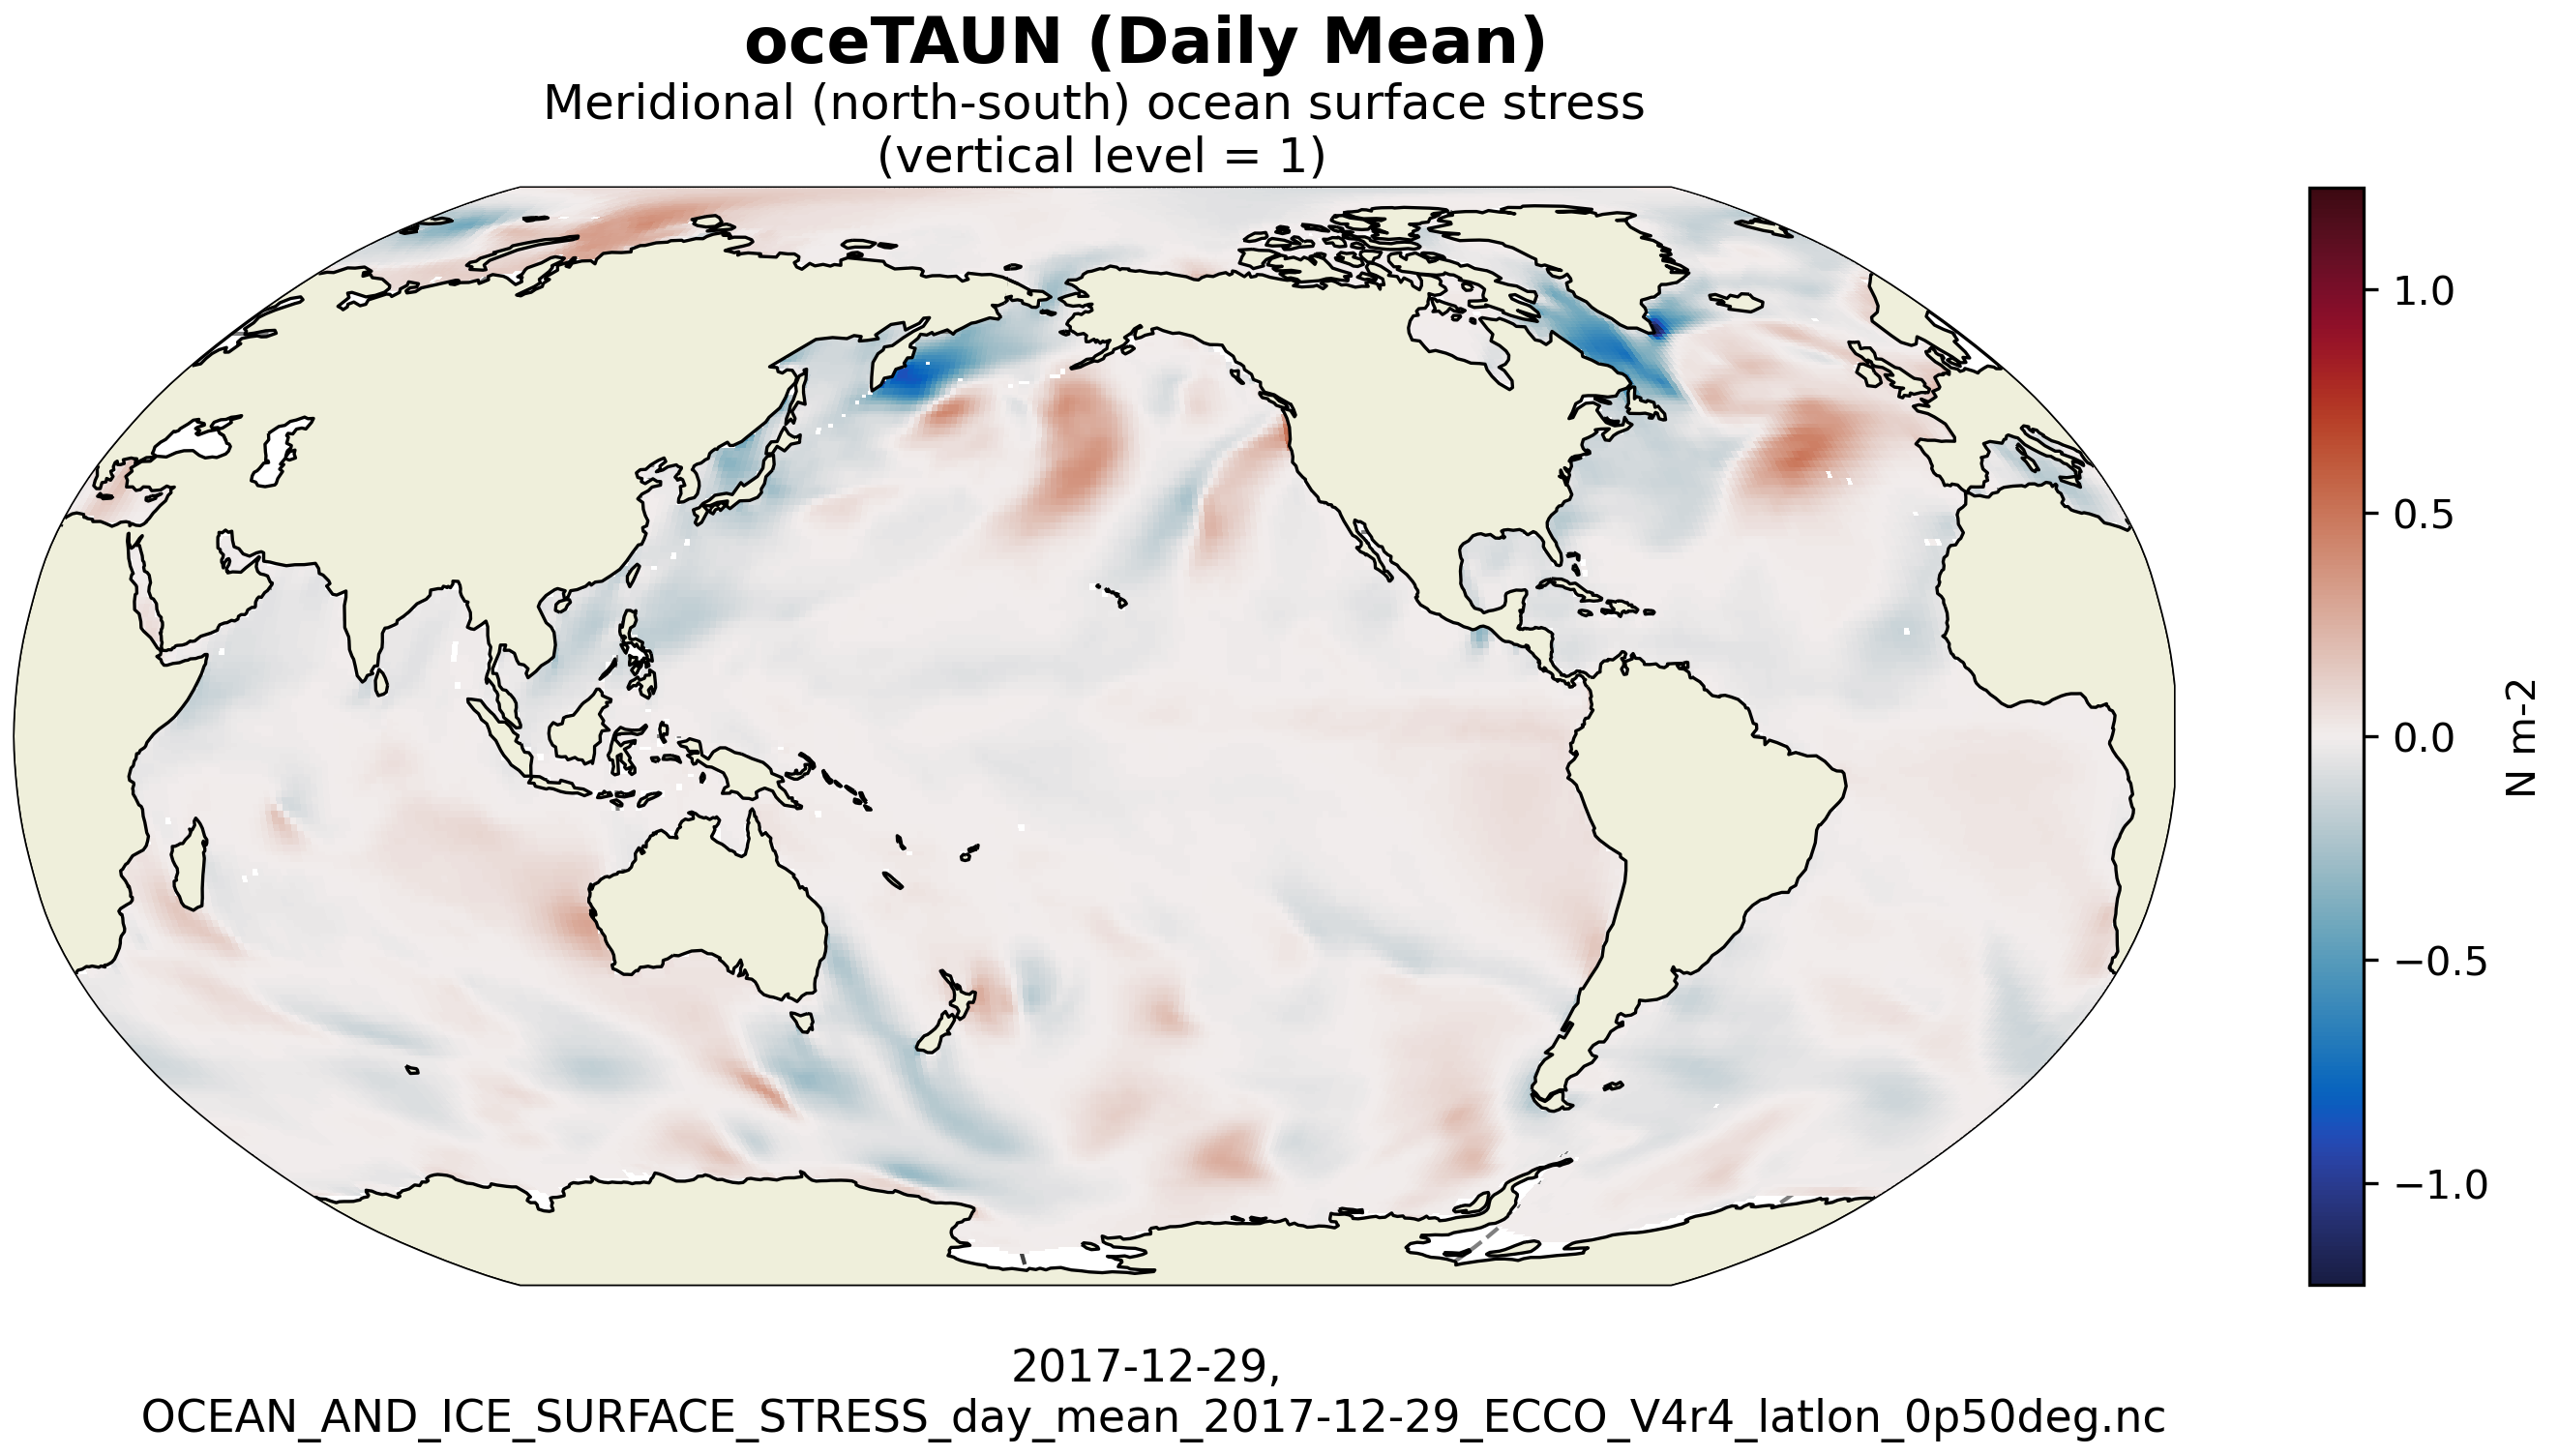
\includegraphics[scale=0.55]{../images/plots/v4r4/latlon_plots/Ocean_and_Sea-Ice_Surface_Stress/oceTAUN.png}
\caption{Dataset: OCEAN\_AND\_ICE\_SURFACE\_STRESS, Variable: oceTAUN}
\label{tab:table-OCEAN_AND_ICE_SURFACE_STRESS_oceTAUN-Plot}
\end{figure}
\newpage
\subsection{Latlon dataset of OCEAN\_BOLUS\_VELOCITY}
\newp
\subsubsection{Overview}
This dataset provides 3D fields of Gent-McWilliams ocean bolus velocity interpolated to a regular 0.5-degree grid from the ECCO Version 4 Release 4 (V4r4) ocean and sea-ice state estimate. The dataset is provided on daily-average and monthly-average time resolution. 
\begin{longtable}{|m{0.15\textwidth}|m{0.64\textwidth}|m{0.12\textwidth}|}
\caption{Coordinates and Variables in the dataset OCEAN\_BOLUS\_VELOCITY}
\label{tab:table-OCEAN_BOLUS_VELOCITY-fields} \\ 
\hline \endhead \hline \endfoot
\rowcolor{lightgray} \multicolumn{1}{|c|}{\textbf{Coordinates}} & \multicolumn{1}{|c|}{\textbf{Description of data coordinates}} &  \multicolumn{1}{|c|}{\textbf{Unit}}\\ \hline
time &Center time of averaging period &--none--  \\ \hline
Z &Depth of grid cell center &m  \\ \hline
latitude &Latitude at grid cell center &degrees\_north  \\ \hline
longitude &Longitude at grid cell center &degrees\_east  \\ \hline
time\_bnds &Time bounds of averaging period &--none--  \\ \hline
latitude\_bnds &Latitude bounds grid cells &--none--  \\ \hline
longitude\_bnds &Longitude bounds grid cells &--none--  \\ \hline
Z\_bnds &Depths of grid cell upper and lower interfaces &--none--  \\ \hline
\rowcolor{lightgray} \multicolumn{1}{|c|}{\textbf{Variables}} & \multicolumn{1}{|c|}{\textbf{Description of data variables}} &  \multicolumn{1}{|c|}{\textbf{Unit}}\\ \hline
EVELSTAR &Gent-mcwilliams zonal (east-west) bolus velocity &m s-1  \\ \hline
NVELSTAR &Gent-mcwilliams meridional (north-south) bolus velocity &m s-1  \\ \hline
WVELSTAR &Gent-mcwilliams vertical bolus velocity &m s-1  \\ \hline
\end{longtable}

\newp
\pagebreak
\subsubsection{Latlon Variable: EVELSTAR}
\begin{longtable}{|m{0.06\textwidth}|m{0.3\textwidth}|m{0.45\textwidth}|m{0.12\textwidth}|}
\caption{Attributes description of the variable 'EVELSTAR' from OCEAN\_BOLUS\_VELOCITY's  dataset.}
\label{tab:table-OCEAN_BOLUS_VELOCITY_EVELSTAR} \\ 
\hline \endhead \hline \endfoot
\rowcolor{lightgray} \textbf{Storage Type} & \textbf{Variable Name} & \textbf{Description} & \textbf{Unit} \\ \hline
float32 & EVELSTAR & Gent-mcwilliams zonal (east-west) bolus velocity & m s-1 \\ \hline
\multicolumn{4}{|c|}{\cellcolor{lightgray}{\textbf{Description of the variable in Common Data language (CDL)}}} \\ \hline
\multicolumn{4}{|c|}{\fontfamily{lmtt}\selectfont{\makecell{\parbox{.95\textwidth}{\vspace*{0.25cm} \footnotesize{float32 EVELSTAR(time, Z, latitude, longitude)\\
\hspace*{0.5cm}EVELSTAR: \_FillValue = 9.96921e+36\\
\hspace*{0.5cm}EVELSTAR: coordinates = time Z\\
\hspace*{0.5cm}EVELSTAR: coverage\_content\_type = modelResult\\
\hspace*{0.5cm}EVELSTAR: long\_name = Gent-McWilliams zonal (east-west) bolus velocity\\
\hspace*{0.5cm}EVELSTAR: standard\_name = eastward sea water velocity due to parameterized mesoscale eddies\\
\hspace*{0.5cm}EVELSTAR: units = m s-1\\
\hspace*{0.5cm}EVELSTAR: valid\_max = 0.7810457944869995\\
\hspace*{0.5cm}EVELSTAR: valid\_min = -0.5832233428955078\\
}}}}} \\ \hline
\rowcolor{lightgray} \multicolumn{4}{|c|}{\textbf{Comments}} \\ \hline
\multicolumn{4}{|p{1\textwidth}|}{\footnotesize{{Zonal (east-west) component of the gent-mcwilliams bolus ocean velocity. note: evelstar is calculated by interpolating the model's x and y components of gm bolus ocean velocity (uvelstar and vvelstar) to tracer cell centers and then finding the zonal components of the interpolated vectors. one should take care when interpreting bolus velocities interpolated from the ecco native model grid because interpolating from the model grid to the lat-lon grid introduces errors. some closed buget calculations require bolus velocity terms on the native model grid.}}} \\ \hline
\end{longtable}

\begin{figure}[H]
\centering
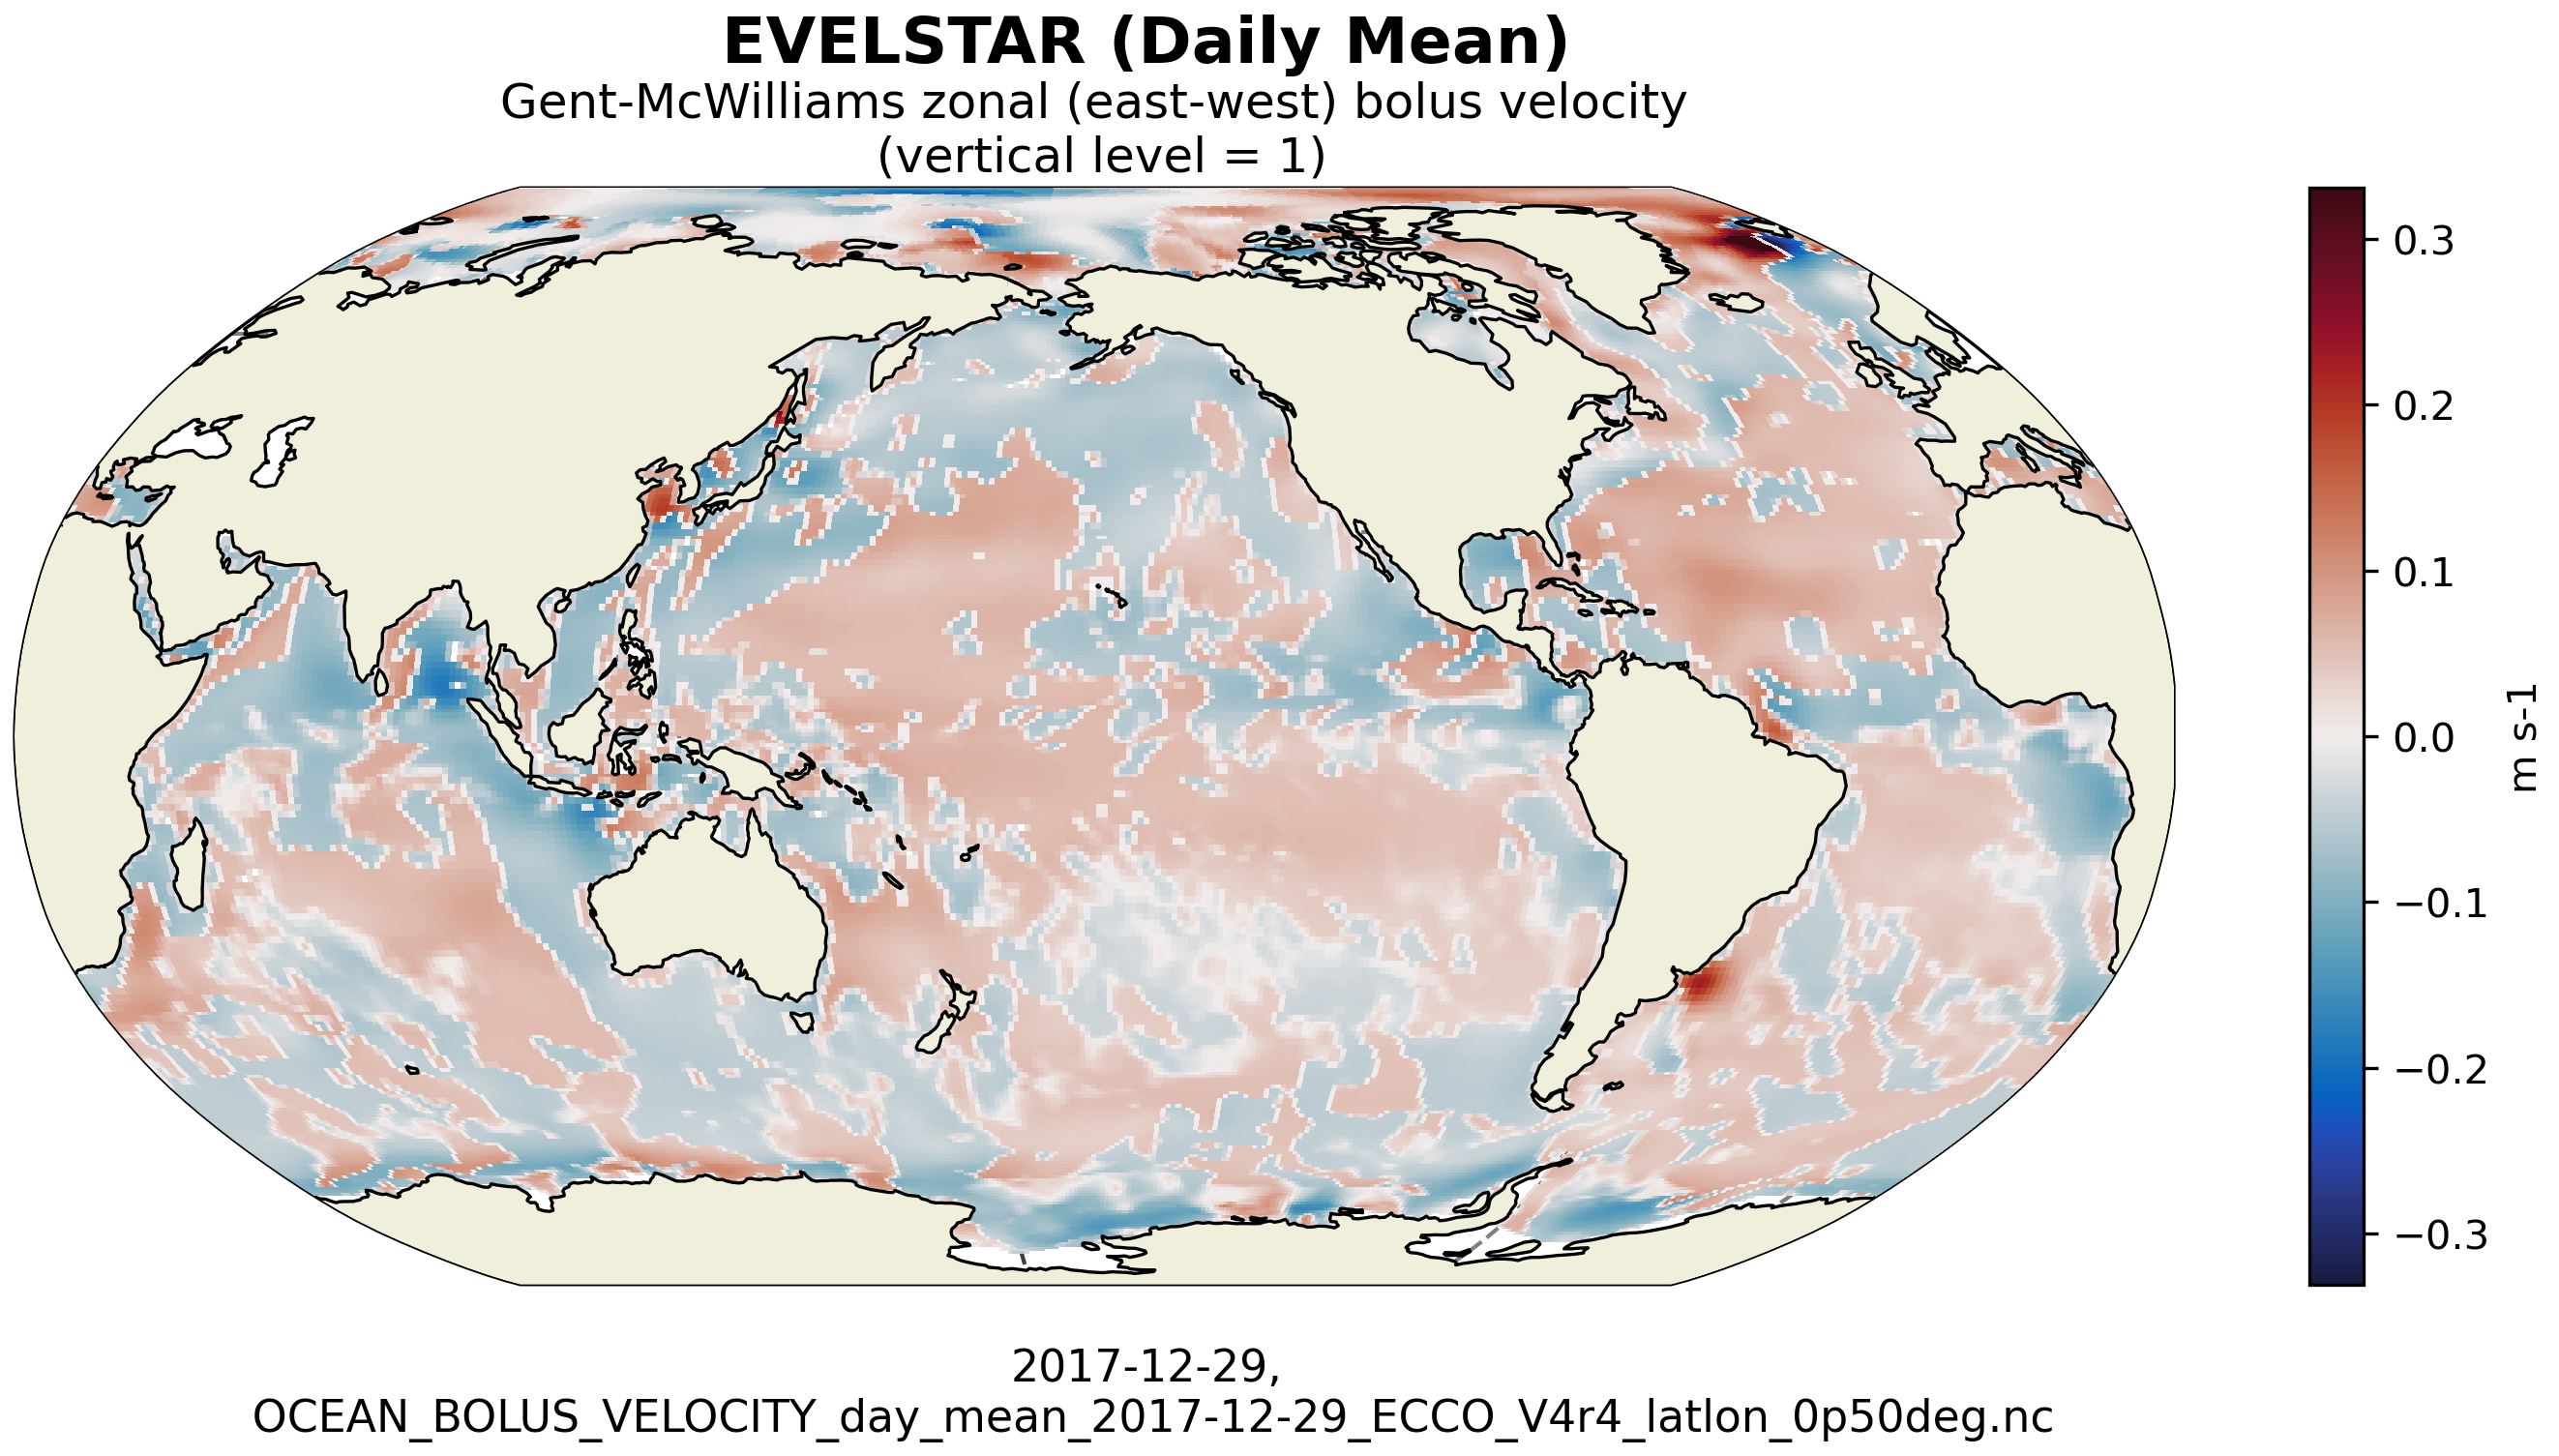
\includegraphics[scale=0.55]{../images/plots/v4r4/latlon_plots/Gent-McWilliams_Ocean_Bolus_Velocity/EVELSTAR.png}
\caption{Dataset: OCEAN\_BOLUS\_VELOCITY, Variable: EVELSTAR}
\label{tab:table-OCEAN_BOLUS_VELOCITY_EVELSTAR-Plot}
\end{figure}
\newpage
\pagebreak
\subsubsection{Latlon Variable: NVELSTAR}
\begin{longtable}{|m{0.06\textwidth}|m{0.3\textwidth}|m{0.45\textwidth}|m{0.12\textwidth}|}
\caption{Attributes description of the variable 'NVELSTAR' from OCEAN\_BOLUS\_VELOCITY's  dataset.}
\label{tab:table-OCEAN_BOLUS_VELOCITY_NVELSTAR} \\ 
\hline \endhead \hline \endfoot
\rowcolor{lightgray} \textbf{Storage Type} & \textbf{Variable Name} & \textbf{Description} & \textbf{Unit} \\ \hline
float32 & NVELSTAR & Gent-mcwilliams meridional (north-south) bolus velocity & m s-1 \\ \hline
\multicolumn{4}{|c|}{\cellcolor{lightgray}{\textbf{Description of the variable in Common Data language (CDL)}}} \\ \hline
\multicolumn{4}{|c|}{\fontfamily{lmtt}\selectfont{\makecell{\parbox{.95\textwidth}{\vspace*{0.25cm} \footnotesize{float32 NVELSTAR(time, Z, latitude, longitude)\\
\hspace*{0.5cm}NVELSTAR: \_FillValue = 9.96921e+36\\
\hspace*{0.5cm}NVELSTAR: coordinates = time Z\\
\hspace*{0.5cm}NVELSTAR: coverage\_content\_type = modelResult\\
\hspace*{0.5cm}NVELSTAR: long\_name = Gent-McWilliams meridional (north-south) bolus velocity\\
\hspace*{0.5cm}NVELSTAR: standard\_name = northward sea water velocity due to parameterized mesoscale eddies\\
\hspace*{0.5cm}NVELSTAR: units = m s-1\\
\hspace*{0.5cm}NVELSTAR: valid\_max = 0.6751338243484497\\
\hspace*{0.5cm}NVELSTAR: valid\_min = -0.6472858190536499\\
}}}}} \\ \hline
\rowcolor{lightgray} \multicolumn{4}{|c|}{\textbf{Comments}} \\ \hline
\multicolumn{4}{|p{1\textwidth}|}{\footnotesize{{Meridional (north-south) component of the gent-mcwilliams bolus ocean velocity. note: nvelstar is calculated by interpolating the model's x and y components of gm bolus ocean velocity (uvelstar and vvelstar) to tracer cell centers and then finding the meridional components of the interpolated vectors.  one should take care when interpreting bolus velocities interpolated from the ecco native model grid because interpolating from the model grid to the lat-lon grid introduces errors. some closed buget calculations require bolus velocity terms on the native model grid}}} \\ \hline
\end{longtable}

\begin{figure}[H]
\centering
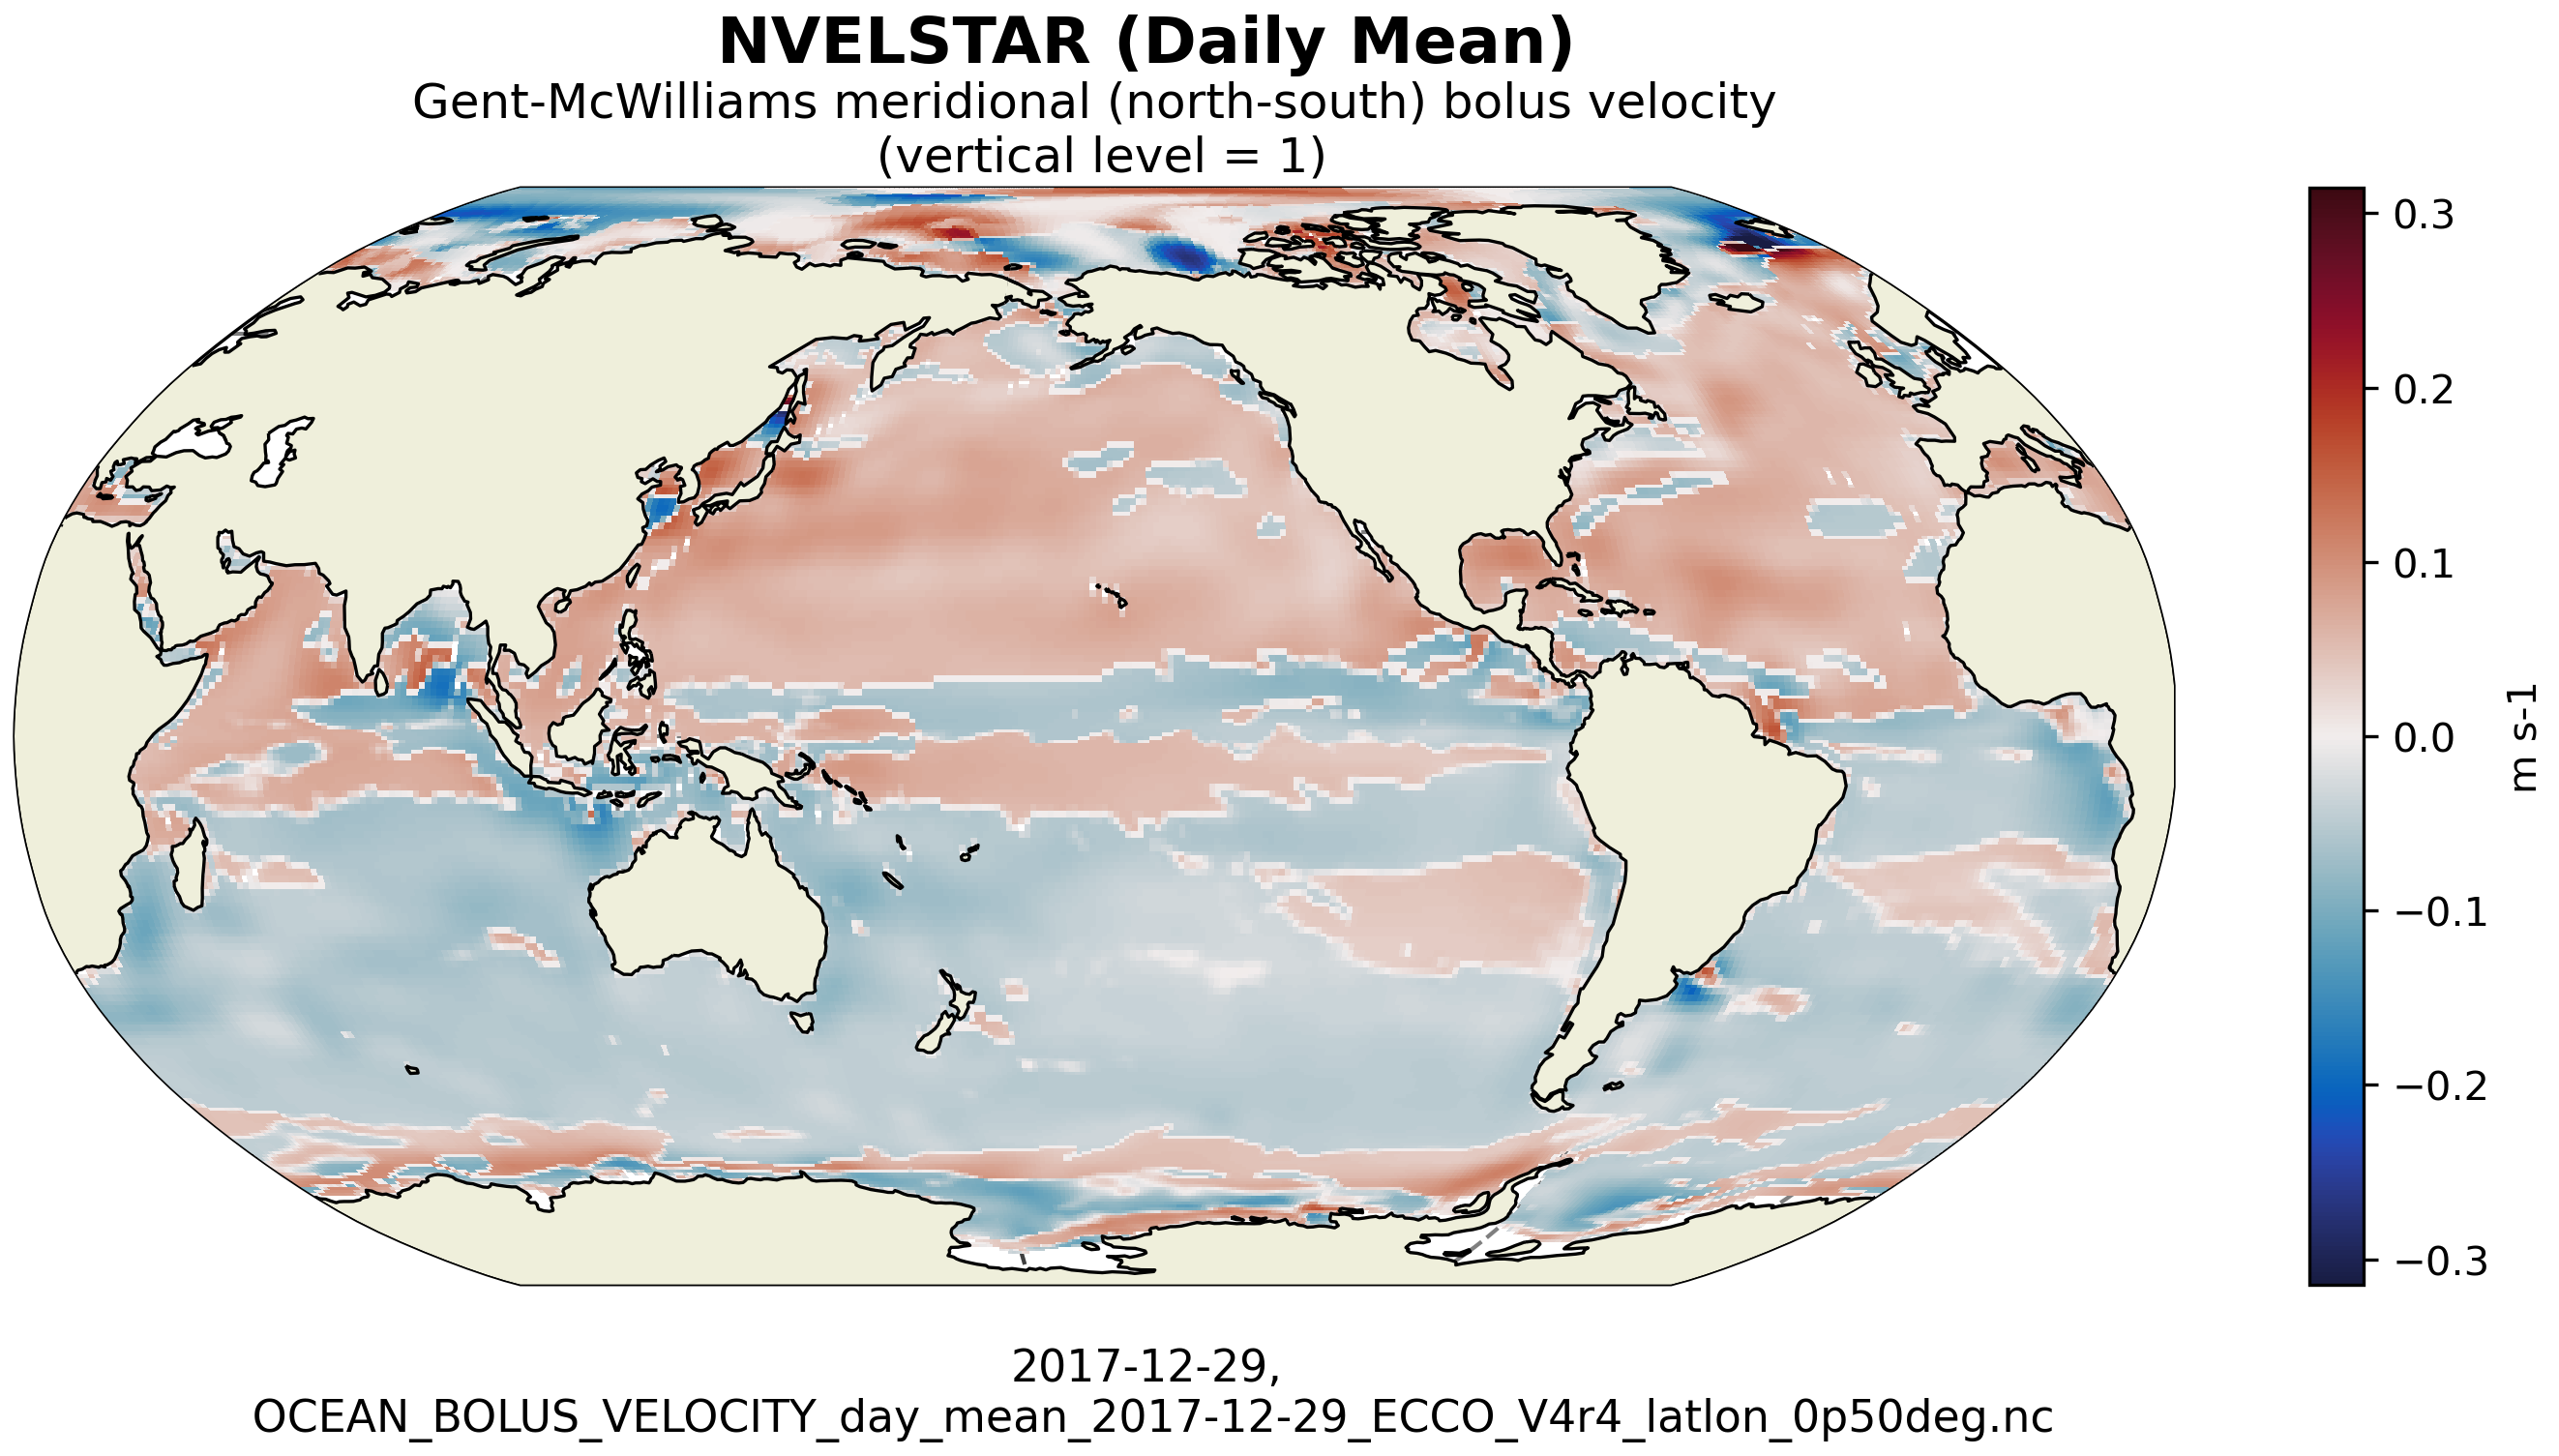
\includegraphics[scale=0.55]{../images/plots/v4r4/latlon_plots/Gent-McWilliams_Ocean_Bolus_Velocity/NVELSTAR.png}
\caption{Dataset: OCEAN\_BOLUS\_VELOCITY, Variable: NVELSTAR}
\label{tab:table-OCEAN_BOLUS_VELOCITY_NVELSTAR-Plot}
\end{figure}
\newpage
\pagebreak
\subsubsection{Latlon Variable: WVELSTAR}
\begin{longtable}{|m{0.06\textwidth}|m{0.3\textwidth}|m{0.45\textwidth}|m{0.12\textwidth}|}
\caption{Attributes description of the variable 'WVELSTAR' from OCEAN\_BOLUS\_VELOCITY's  dataset.}
\label{tab:table-OCEAN_BOLUS_VELOCITY_WVELSTAR} \\ 
\hline \endhead \hline \endfoot
\rowcolor{lightgray} \textbf{Storage Type} & \textbf{Variable Name} & \textbf{Description} & \textbf{Unit} \\ \hline
float32 & WVELSTAR & Gent-mcwilliams vertical bolus velocity & m s-1 \\ \hline
\multicolumn{4}{|c|}{\cellcolor{lightgray}{\textbf{Description of the variable in Common Data language (CDL)}}} \\ \hline
\multicolumn{4}{|c|}{\fontfamily{lmtt}\selectfont{\makecell{\parbox{.95\textwidth}{\vspace*{0.25cm} \footnotesize{float32 WVELSTAR(time, Z, latitude, longitude)\\
\hspace*{0.5cm}WVELSTAR: \_FillValue = 9.96921e+36\\
\hspace*{0.5cm}WVELSTAR: coordinates = time Z\\
\hspace*{0.5cm}WVELSTAR: coverage\_content\_type = modelResult\\
\hspace*{0.5cm}WVELSTAR: direction = >0 decreases volume\\
\hspace*{0.5cm}WVELSTAR: long\_name = Gent-McWilliams vertical bolus velocity\\
\hspace*{0.5cm}WVELSTAR: standard\_name = upward sea water velocity due to parameterized mesoscale eddies\\
\hspace*{0.5cm}WVELSTAR: units = m s-1\\
\hspace*{0.5cm}WVELSTAR: valid\_max = 0.0004019034677185118\\
\hspace*{0.5cm}WVELSTAR: valid\_min = -0.00037936007720418274\\
}}}}} \\ \hline
\rowcolor{lightgray} \multicolumn{4}{|c|}{\textbf{Comments}} \\ \hline
\multicolumn{4}{|p{1\textwidth}|}{\footnotesize{{Vertical component of the gent-mcwilliams bolus ocean velocity. note: in the arakawa-c grid used in ecco v4r4, vertical velocities are staggered relative to the tracer cell centers with values at the top and bottom faces of each grid cell.}}} \\ \hline
\end{longtable}

\begin{figure}[H]
\centering
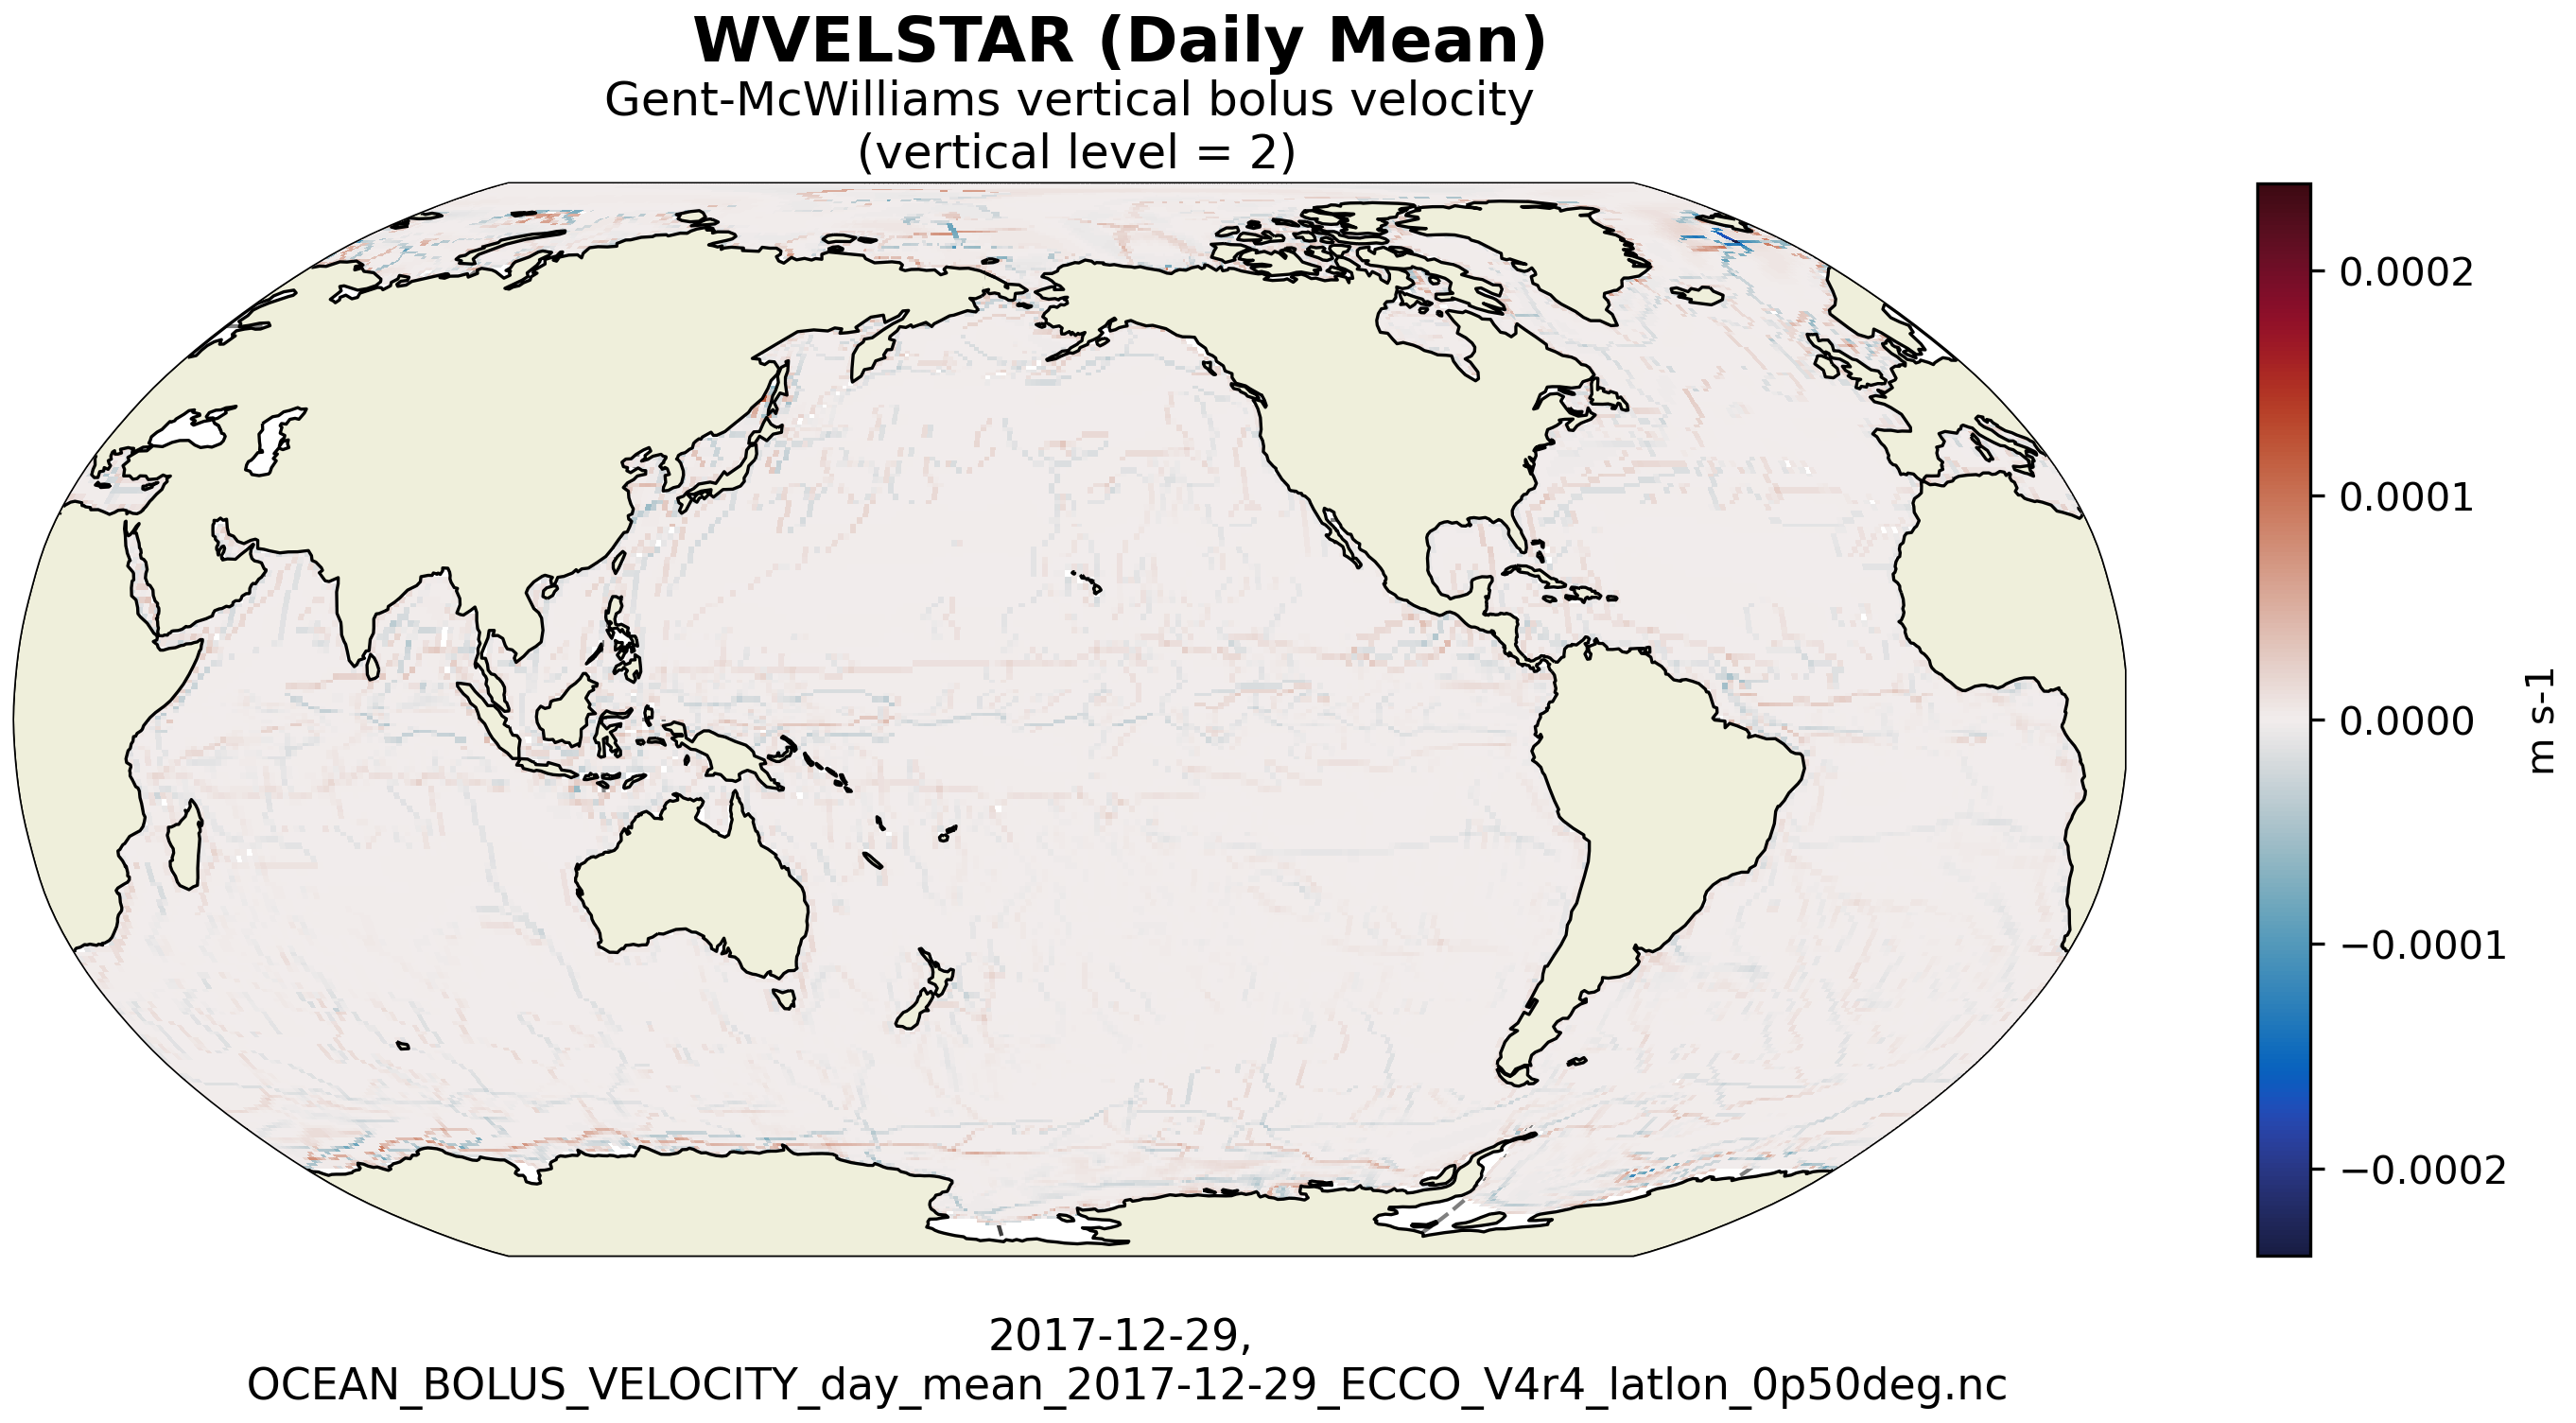
\includegraphics[scale=0.55]{../images/plots/v4r4/latlon_plots/Gent-McWilliams_Ocean_Bolus_Velocity/WVELSTAR.png}
\caption{Dataset: OCEAN\_BOLUS\_VELOCITY, Variable: WVELSTAR}
\label{tab:table-OCEAN_BOLUS_VELOCITY_WVELSTAR-Plot}
\end{figure}
\newpage
\subsection{Latlon dataset of OCEAN\_BOTTOM\_PRESSURE}
\newp
\subsubsection{Overview}
This dataset provides 2D fields of ocean bottom pressure interpolated to a regular 0.5-degree grid from the ECCO Version 4 Release 4 (V4r4) ocean and sea-ice state estimate. The dataset is provided on daily-average and monthly-average time resolution. Ocean bottom pressure given in equivalent water thickness excluding (OBP) and including (OBPGMAP) the contribution from global mean atmospheric pressure. 
\begin{longtable}{|m{0.15\textwidth}|m{0.64\textwidth}|m{0.12\textwidth}|}
\caption{Coordinates and Variables in the dataset OCEAN\_BOTTOM\_PRESSURE}
\label{tab:table-OCEAN_BOTTOM_PRESSURE-fields} \\ 
\hline \endhead \hline \endfoot
\rowcolor{lightgray} \multicolumn{1}{|c|}{\textbf{Coordinates}} & \multicolumn{1}{|c|}{\textbf{Description of data coordinates}} &  \multicolumn{1}{|c|}{\textbf{Unit}}\\ \hline
time &Center time of averaging period &--none--  \\ \hline
latitude &Latitude at grid cell center &degrees\_north  \\ \hline
longitude &Longitude at grid cell center &degrees\_east  \\ \hline
time\_bnds &Time bounds of averaging period &--none--  \\ \hline
latitude\_bnds &Latitude bounds grid cells &--none--  \\ \hline
longitude\_bnds &Longitude bounds grid cells &--none--  \\ \hline
\rowcolor{lightgray} \multicolumn{1}{|c|}{\textbf{Variables}} & \multicolumn{1}{|c|}{\textbf{Description of data variables}} &  \multicolumn{1}{|c|}{\textbf{Unit}}\\ \hline
OBP &Ocean bottom pressure given as equivalent water thickness &m  \\ \hline
OBPGMAP &Ocean bottom pressure given as equivalent water thickness, includes global mean atmospheric pressure &m  \\ \hline
\end{longtable}

\newp
\pagebreak
\subsubsection{Latlon Variable: OBP}
\begin{longtable}{|m{0.06\textwidth}|m{0.3\textwidth}|m{0.45\textwidth}|m{0.12\textwidth}|}
\caption{Attributes description of the variable 'OBP' from OCEAN\_BOTTOM\_PRESSURE's  dataset.}
\label{tab:table-OCEAN_BOTTOM_PRESSURE_OBP} \\ 
\hline \endhead \hline \endfoot
\rowcolor{lightgray} \textbf{Storage Type} & \textbf{Variable Name} & \textbf{Description} & \textbf{Unit} \\ \hline
float32 & OBP & Ocean bottom pressure given as equivalent water thickness & m \\ \hline
\multicolumn{4}{|c|}{\cellcolor{lightgray}{\textbf{Description of the variable in Common Data language (CDL)}}} \\ \hline
\multicolumn{4}{|c|}{\fontfamily{lmtt}\selectfont{\makecell{\parbox{.95\textwidth}{\vspace*{0.25cm} \footnotesize{float32 OBP(time, latitude, longitude)\\
\hspace*{0.5cm}OBP: \_FillValue = 9.96921e+36\\
\hspace*{0.5cm}OBP: coordinates = time\\
\hspace*{0.5cm}OBP: coverage\_content\_type = modelResult\\
\hspace*{0.5cm}OBP: long\_name = Ocean bottom pressure given as equivalent water thickness\\
\hspace*{0.5cm}OBP: units = m\\
\hspace*{0.5cm}OBP: valid\_max = 72.1243667602539\\
\hspace*{0.5cm}OBP: valid\_min = -2.544442892074585\\
}}}}} \\ \hline
\rowcolor{lightgray} \multicolumn{4}{|c|}{\textbf{Comments}} \\ \hline
\multicolumn{4}{|p{1\textwidth}|}{\footnotesize{{Obp excludes the contribution from global mean atmospheric pressure and is therefore suitable for comparisons with grace data products. obp is calculated as follows. first, we calculate ocean hydrostatic bottom pressure anomaly, phibot, with phibot = p\_b/rhoconst - gh(t), where p\_b = model ocean hydrostatic bottom pressure, rhoconst = reference density (1029 kg m-3), g is acceleration due to gravity (9.81 m s-2), and h(t) is model depth at time t. then, obp = phibot/g + corrections for i) global mean steric sea level changes related to density changes in the boussinesq volume-conserving model (greatbatch correction, see stergloh) and ii) global mean atmospheric pressure variations. use obp for comparisons with ocean bottom pressure data products that have been corrected for global mean atmospheric pressure variations. grace data typically are corrected for global mean atmospheric pressure variations. in contrast, ocean bottom pressure gauge data typically are not corrected for global mean atmospheric pressure variations.}}} \\ \hline
\end{longtable}

\begin{figure}[H]
\centering
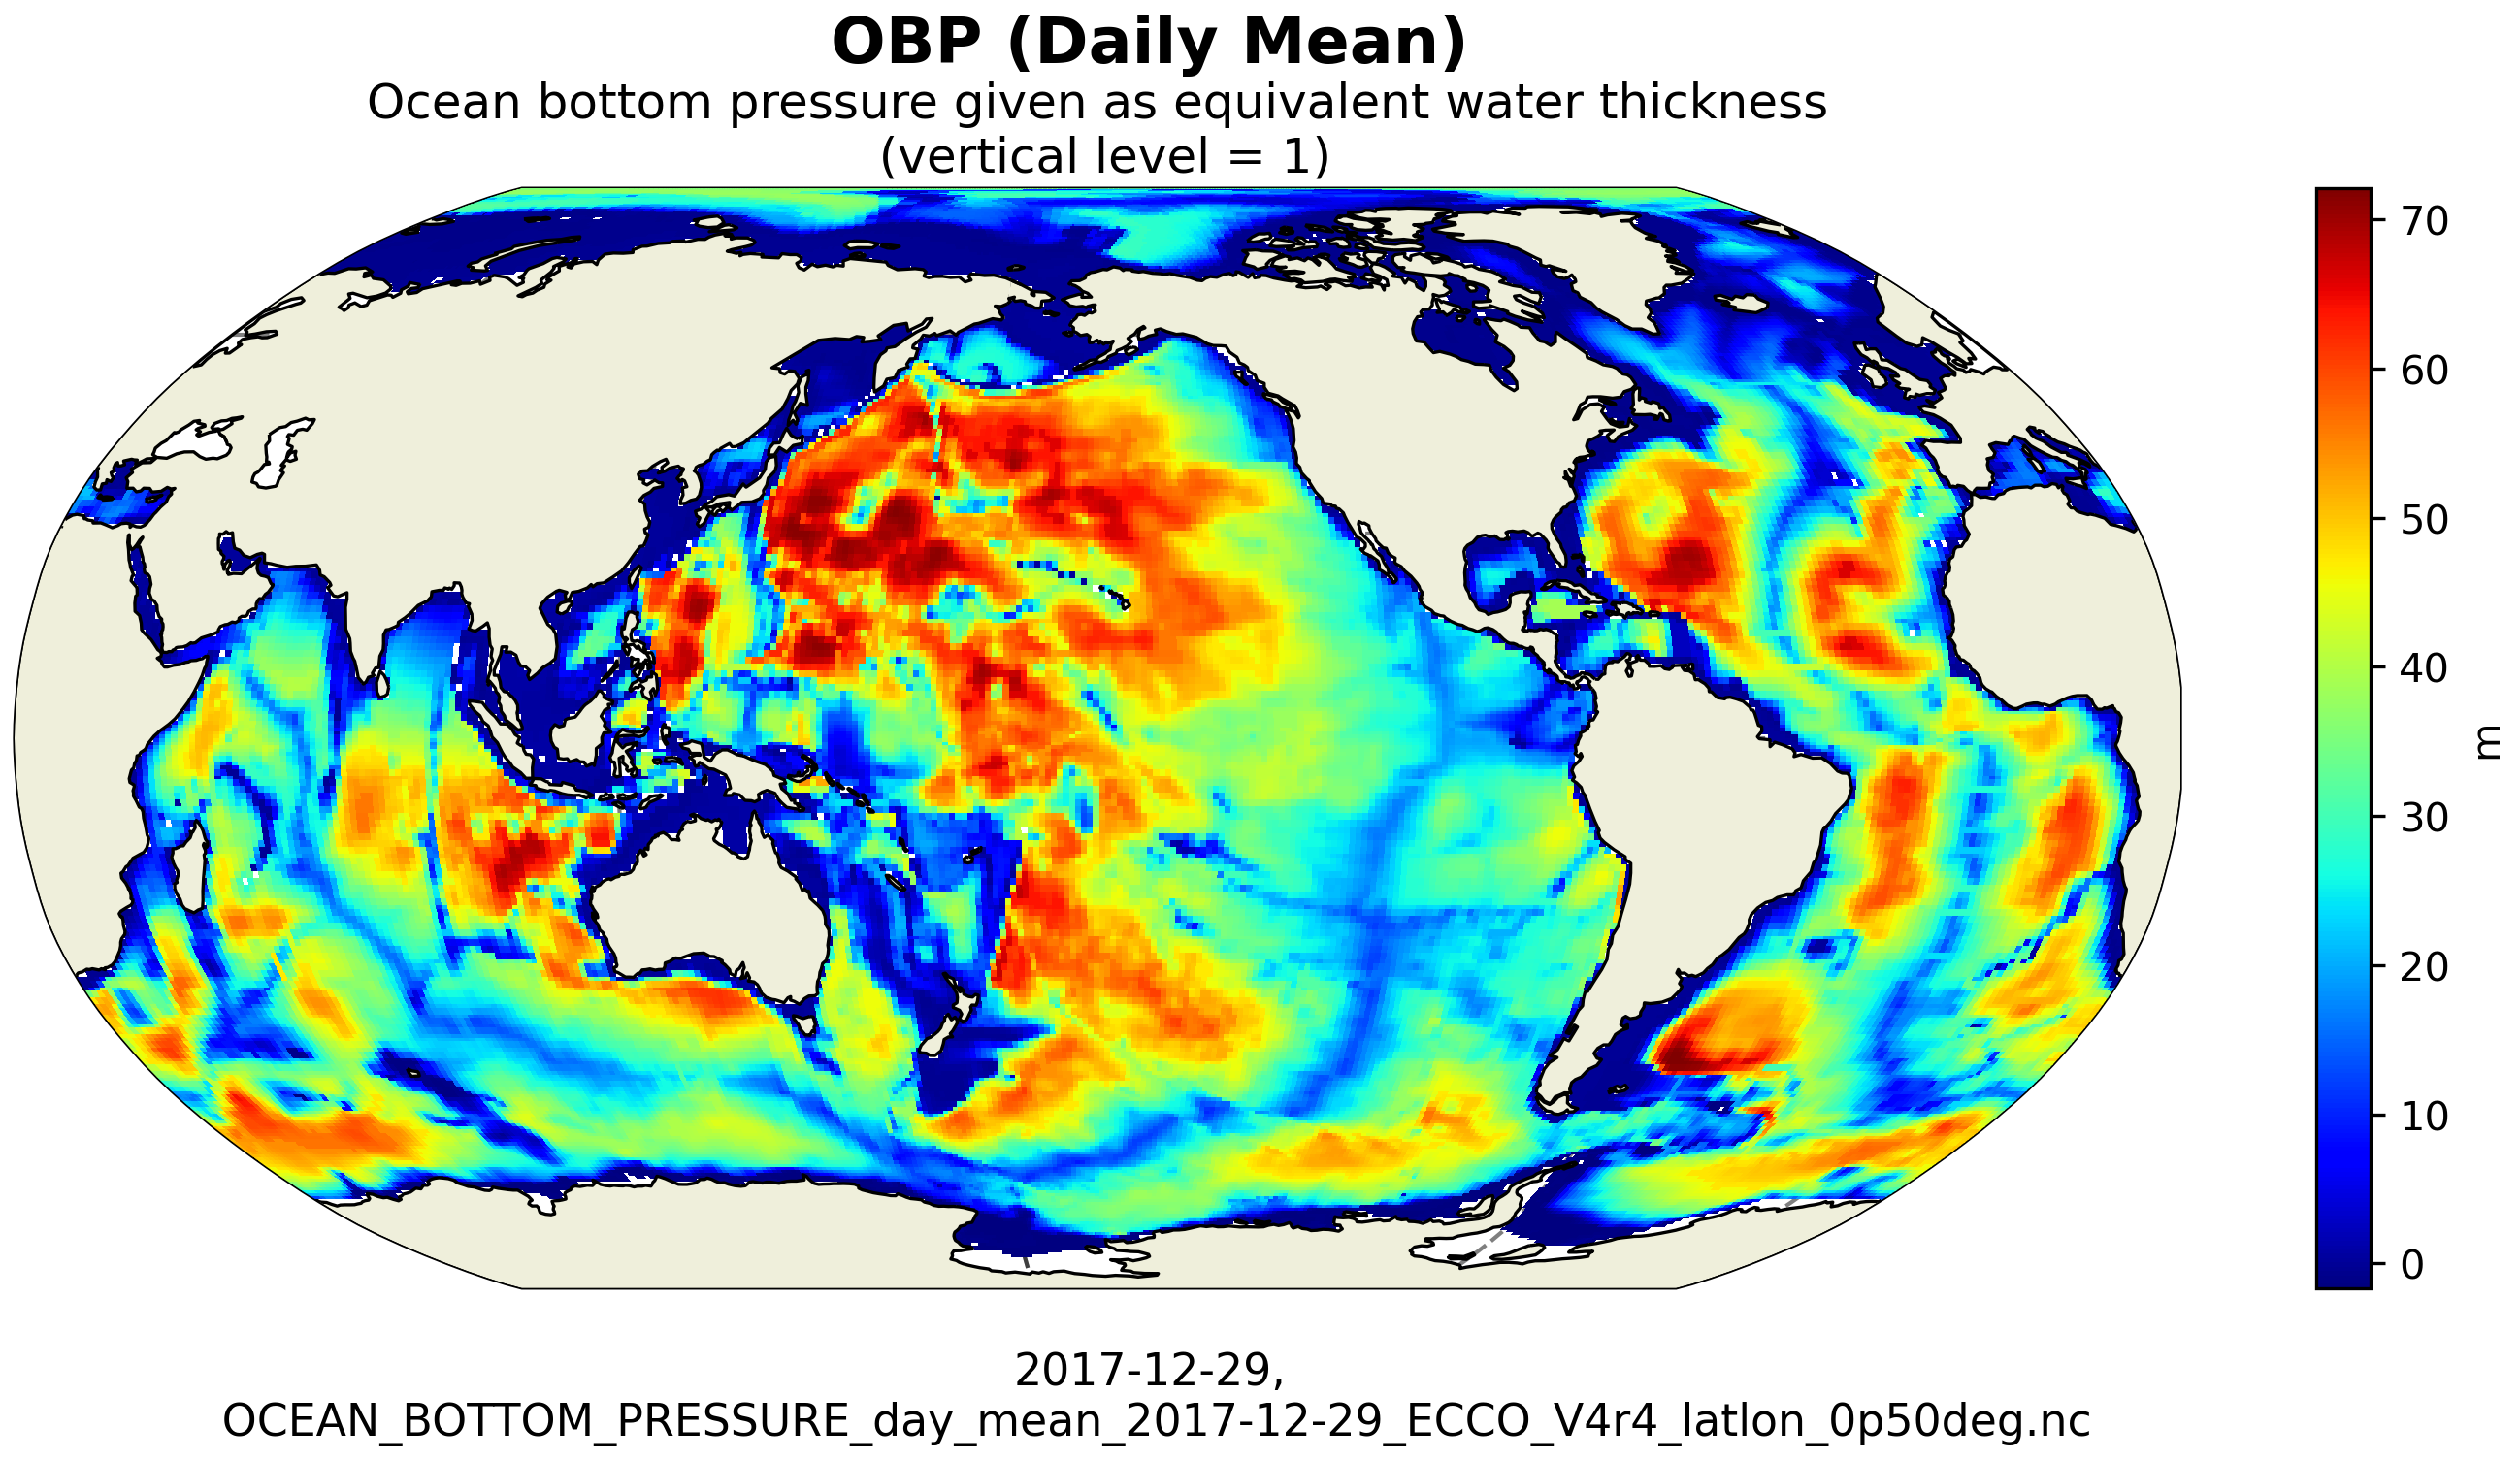
\includegraphics[scale=0.55]{../images/plots/v4r4/latlon_plots/Ocean_Bottom_Pressure/OBP.png}
\caption{Dataset: OCEAN\_BOTTOM\_PRESSURE, Variable: OBP}
\label{tab:table-OCEAN_BOTTOM_PRESSURE_OBP-Plot}
\end{figure}
\newpage
\pagebreak
\subsubsection{Latlon Variable: OBPGMAP}
\begin{longtable}{|m{0.06\textwidth}|m{0.3\textwidth}|m{0.45\textwidth}|m{0.12\textwidth}|}
\caption{Attributes description of the variable 'OBPGMAP' from OCEAN\_BOTTOM\_PRESSURE's  dataset.}
\label{tab:table-OCEAN_BOTTOM_PRESSURE_OBPGMAP} \\ 
\hline \endhead \hline \endfoot
\rowcolor{lightgray} \textbf{Storage Type} & \textbf{Variable Name} & \textbf{Description} & \textbf{Unit} \\ \hline
float32 & OBPGMAP & Ocean bottom pressure given as equivalent water thickness, includes global mean atmospheric pressure & m \\ \hline
\multicolumn{4}{|c|}{\cellcolor{lightgray}{\textbf{Description of the variable in Common Data language (CDL)}}} \\ \hline
\multicolumn{4}{|c|}{\fontfamily{lmtt}\selectfont{\makecell{\parbox{.95\textwidth}{\vspace*{0.25cm} \footnotesize{float32 OBPGMAP(time, latitude, longitude)\\
\hspace*{0.5cm}OBPGMAP: \_FillValue = 9.96921e+36\\
\hspace*{0.5cm}OBPGMAP: coordinates = time\\
\hspace*{0.5cm}OBPGMAP: coverage\_content\_type = modelResult\\
\hspace*{0.5cm}OBPGMAP: long\_name = Ocean bottom pressure given as equivalent water thickness, includes global mean atmospheric pressure\\
\hspace*{0.5cm}OBPGMAP: units = m\\
\hspace*{0.5cm}OBPGMAP: valid\_max = 82.14805603027344\\
\hspace*{0.5cm}OBPGMAP: valid\_min = 7.395928859710693\\
}}}}} \\ \hline
\rowcolor{lightgray} \multicolumn{4}{|c|}{\textbf{Comments}} \\ \hline
\multicolumn{4}{|p{1\textwidth}|}{\footnotesize{{Obpgmap includes the contribution from global mean atmospheric pressure and is therefore suitable for comparisons with ocean bottom pressure gauge data products. obpgmap is calculated as follows. first, we calculate ocean hydrostatic bottom pressure anomaly, phibot, with phibot = p\_b/rhoconst - gh(t), where p\_b = model ocean hydrostatic bottom pressure, rhoconst = reference density (1029 kg m-3), g is acceleration due to gravity (9.81 m s-2), and h(t) is model depth at time t. then, obpgmap= phibot/g + corrections for global mean steric sea level changes related to density changes in the boussinesq volume-conserving model (greatbatch correction, see stergloh). use obpgmap for comparisons with ocean bottom pressure data products that have not been corrected for global mean atmospheric pressure variations. grace data typically are corrected for global mean atmospheric pressure variations. in contrast, ocean bottom pressure gauge data typically are not corrected for global mean atmospheric pressure variations.}}} \\ \hline
\end{longtable}

\begin{figure}[H]
\centering
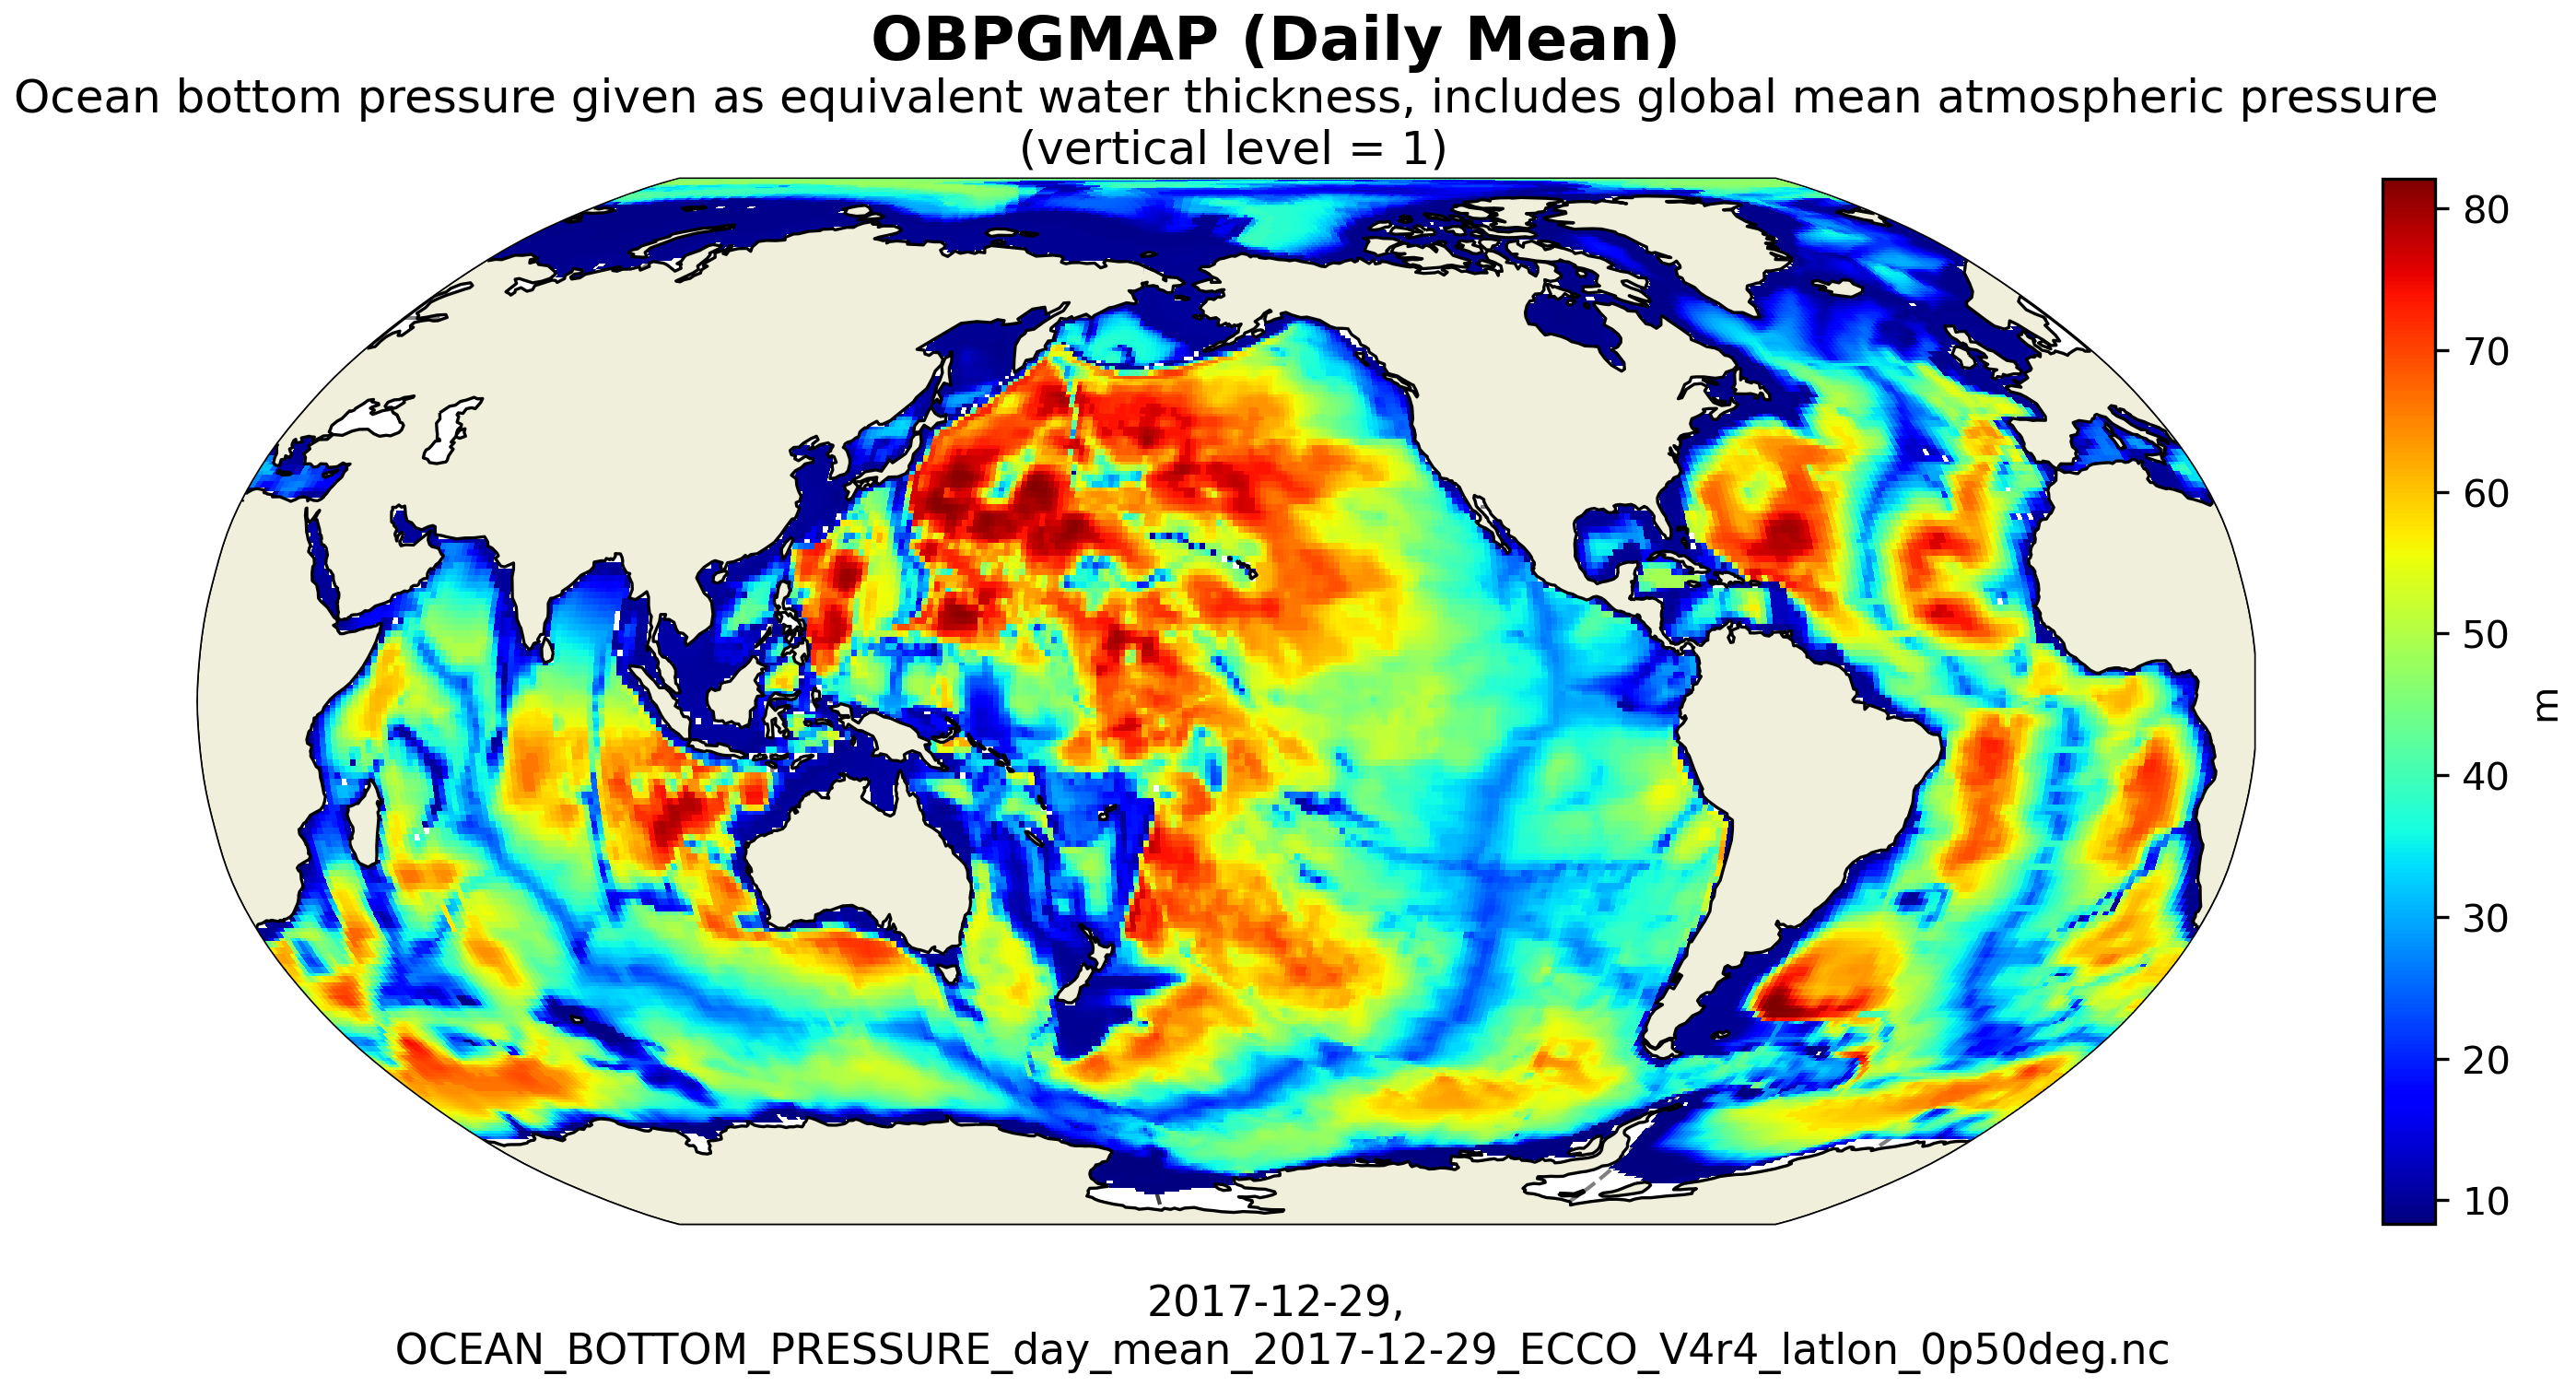
\includegraphics[scale=0.55]{../images/plots/v4r4/latlon_plots/Ocean_Bottom_Pressure/OBPGMAP.png}
\caption{Dataset: OCEAN\_BOTTOM\_PRESSURE, Variable: OBPGMAP}
\label{tab:table-OCEAN_BOTTOM_PRESSURE_OBPGMAP-Plot}
\end{figure}
\newpage
\subsection{Latlon dataset of OCEAN\_DENS\_STRAT\_PRESS}
\newp
\subsubsection{Overview}
This dataset provides 3D fields of ocean density, stratification, and hydrostatic pressure interpolated to a regular0.5-degree grid from the ECCO Version 4 Release 4 (V4r4) ocean and sea-ice state estimate. The dataset is provided on daily-average and monthly-average time resolution. 
\begin{longtable}{|m{0.15\textwidth}|m{0.64\textwidth}|m{0.12\textwidth}|}
\caption{Coordinates and Variables in the dataset OCEAN\_DENS\_STRAT\_PRESS}
\label{tab:table-OCEAN_DENS_STRAT_PRESS-fields} \\ 
\hline \endhead \hline \endfoot
\rowcolor{lightgray} \multicolumn{1}{|c|}{\textbf{Coordinates}} & \multicolumn{1}{|c|}{\textbf{Description of data coordinates}} &  \multicolumn{1}{|c|}{\textbf{Unit}}\\ \hline
time &Center time of averaging period &--none--  \\ \hline
Z &Depth of grid cell center &m  \\ \hline
latitude &Latitude at grid cell center &degrees\_north  \\ \hline
longitude &Longitude at grid cell center &degrees\_east  \\ \hline
time\_bnds &Time bounds of averaging period &--none--  \\ \hline
latitude\_bnds &Latitude bounds grid cells &--none--  \\ \hline
longitude\_bnds &Longitude bounds grid cells &--none--  \\ \hline
Z\_bnds &Depths of grid cell upper and lower interfaces &--none--  \\ \hline
\rowcolor{lightgray} \multicolumn{1}{|c|}{\textbf{Variables}} & \multicolumn{1}{|c|}{\textbf{Description of data variables}} &  \multicolumn{1}{|c|}{\textbf{Unit}}\\ \hline
RHOAnoma &In-situ seawater density anomaly &kg m-3  \\ \hline
DRHODR &Density stratification &kg m-3 m-1  \\ \hline
PHIHYD &Ocean hydrostatic pressure anomaly &m2 s-2  \\ \hline
\end{longtable}

\newp
\pagebreak
\subsubsection{Latlon Variable: DRHODR}
\begin{longtable}{|m{0.06\textwidth}|m{0.3\textwidth}|m{0.45\textwidth}|m{0.12\textwidth}|}
\caption{Attributes description of the variable 'DRHODR' from OCEAN\_DENS\_STRAT\_PRESS's  dataset.}
\label{tab:table-OCEAN_DENS_STRAT_PRESS_DRHODR} \\ 
\hline \endhead \hline \endfoot
\rowcolor{lightgray} \textbf{Storage Type} & \textbf{Variable Name} & \textbf{Description} & \textbf{Unit} \\ \hline
float32 & DRHODR & Density stratification & kg m-3 m-1 \\ \hline
\multicolumn{4}{|c|}{\cellcolor{lightgray}{\textbf{Description of the variable in Common Data language (CDL)}}} \\ \hline
\multicolumn{4}{|c|}{\fontfamily{lmtt}\selectfont{\makecell{\parbox{.95\textwidth}{\vspace*{0.25cm} \footnotesize{float32 DRHODR(time, Z, latitude, longitude)\\
\hspace*{0.5cm}DRHODR: \_FillValue = 9.96921e+36\\
\hspace*{0.5cm}DRHODR: coordinates = time Z\\
\hspace*{0.5cm}DRHODR: coverage\_content\_type = modelResult\\
\hspace*{0.5cm}DRHODR: long\_name = Density stratification\\
\hspace*{0.5cm}DRHODR: units = kg m-3 m-1\\
\hspace*{0.5cm}DRHODR: valid\_max = 0.011617615818977356\\
\hspace*{0.5cm}DRHODR: valid\_min = -0.8687265515327454\\
}}}}} \\ \hline
\rowcolor{lightgray} \multicolumn{4}{|c|}{\textbf{Comments}} \\ \hline
\multicolumn{4}{|p{1\textwidth}|}{\footnotesize{{Density stratification: d(sigma) d z-1. note: density computations are done with in-situ density. the vertical derivatives of in-situ density and locally-referenced potential density are identical  the equation of state is a modified unesco formula by jackett and mcdougall (1995), which uses the model variable potential temperature as input assuming a horizontally and temporally constant pressure of \$p\_0=-g 
ho\_\{0\} z\$.}}} \\ \hline
\end{longtable}

\begin{figure}[H]
\centering
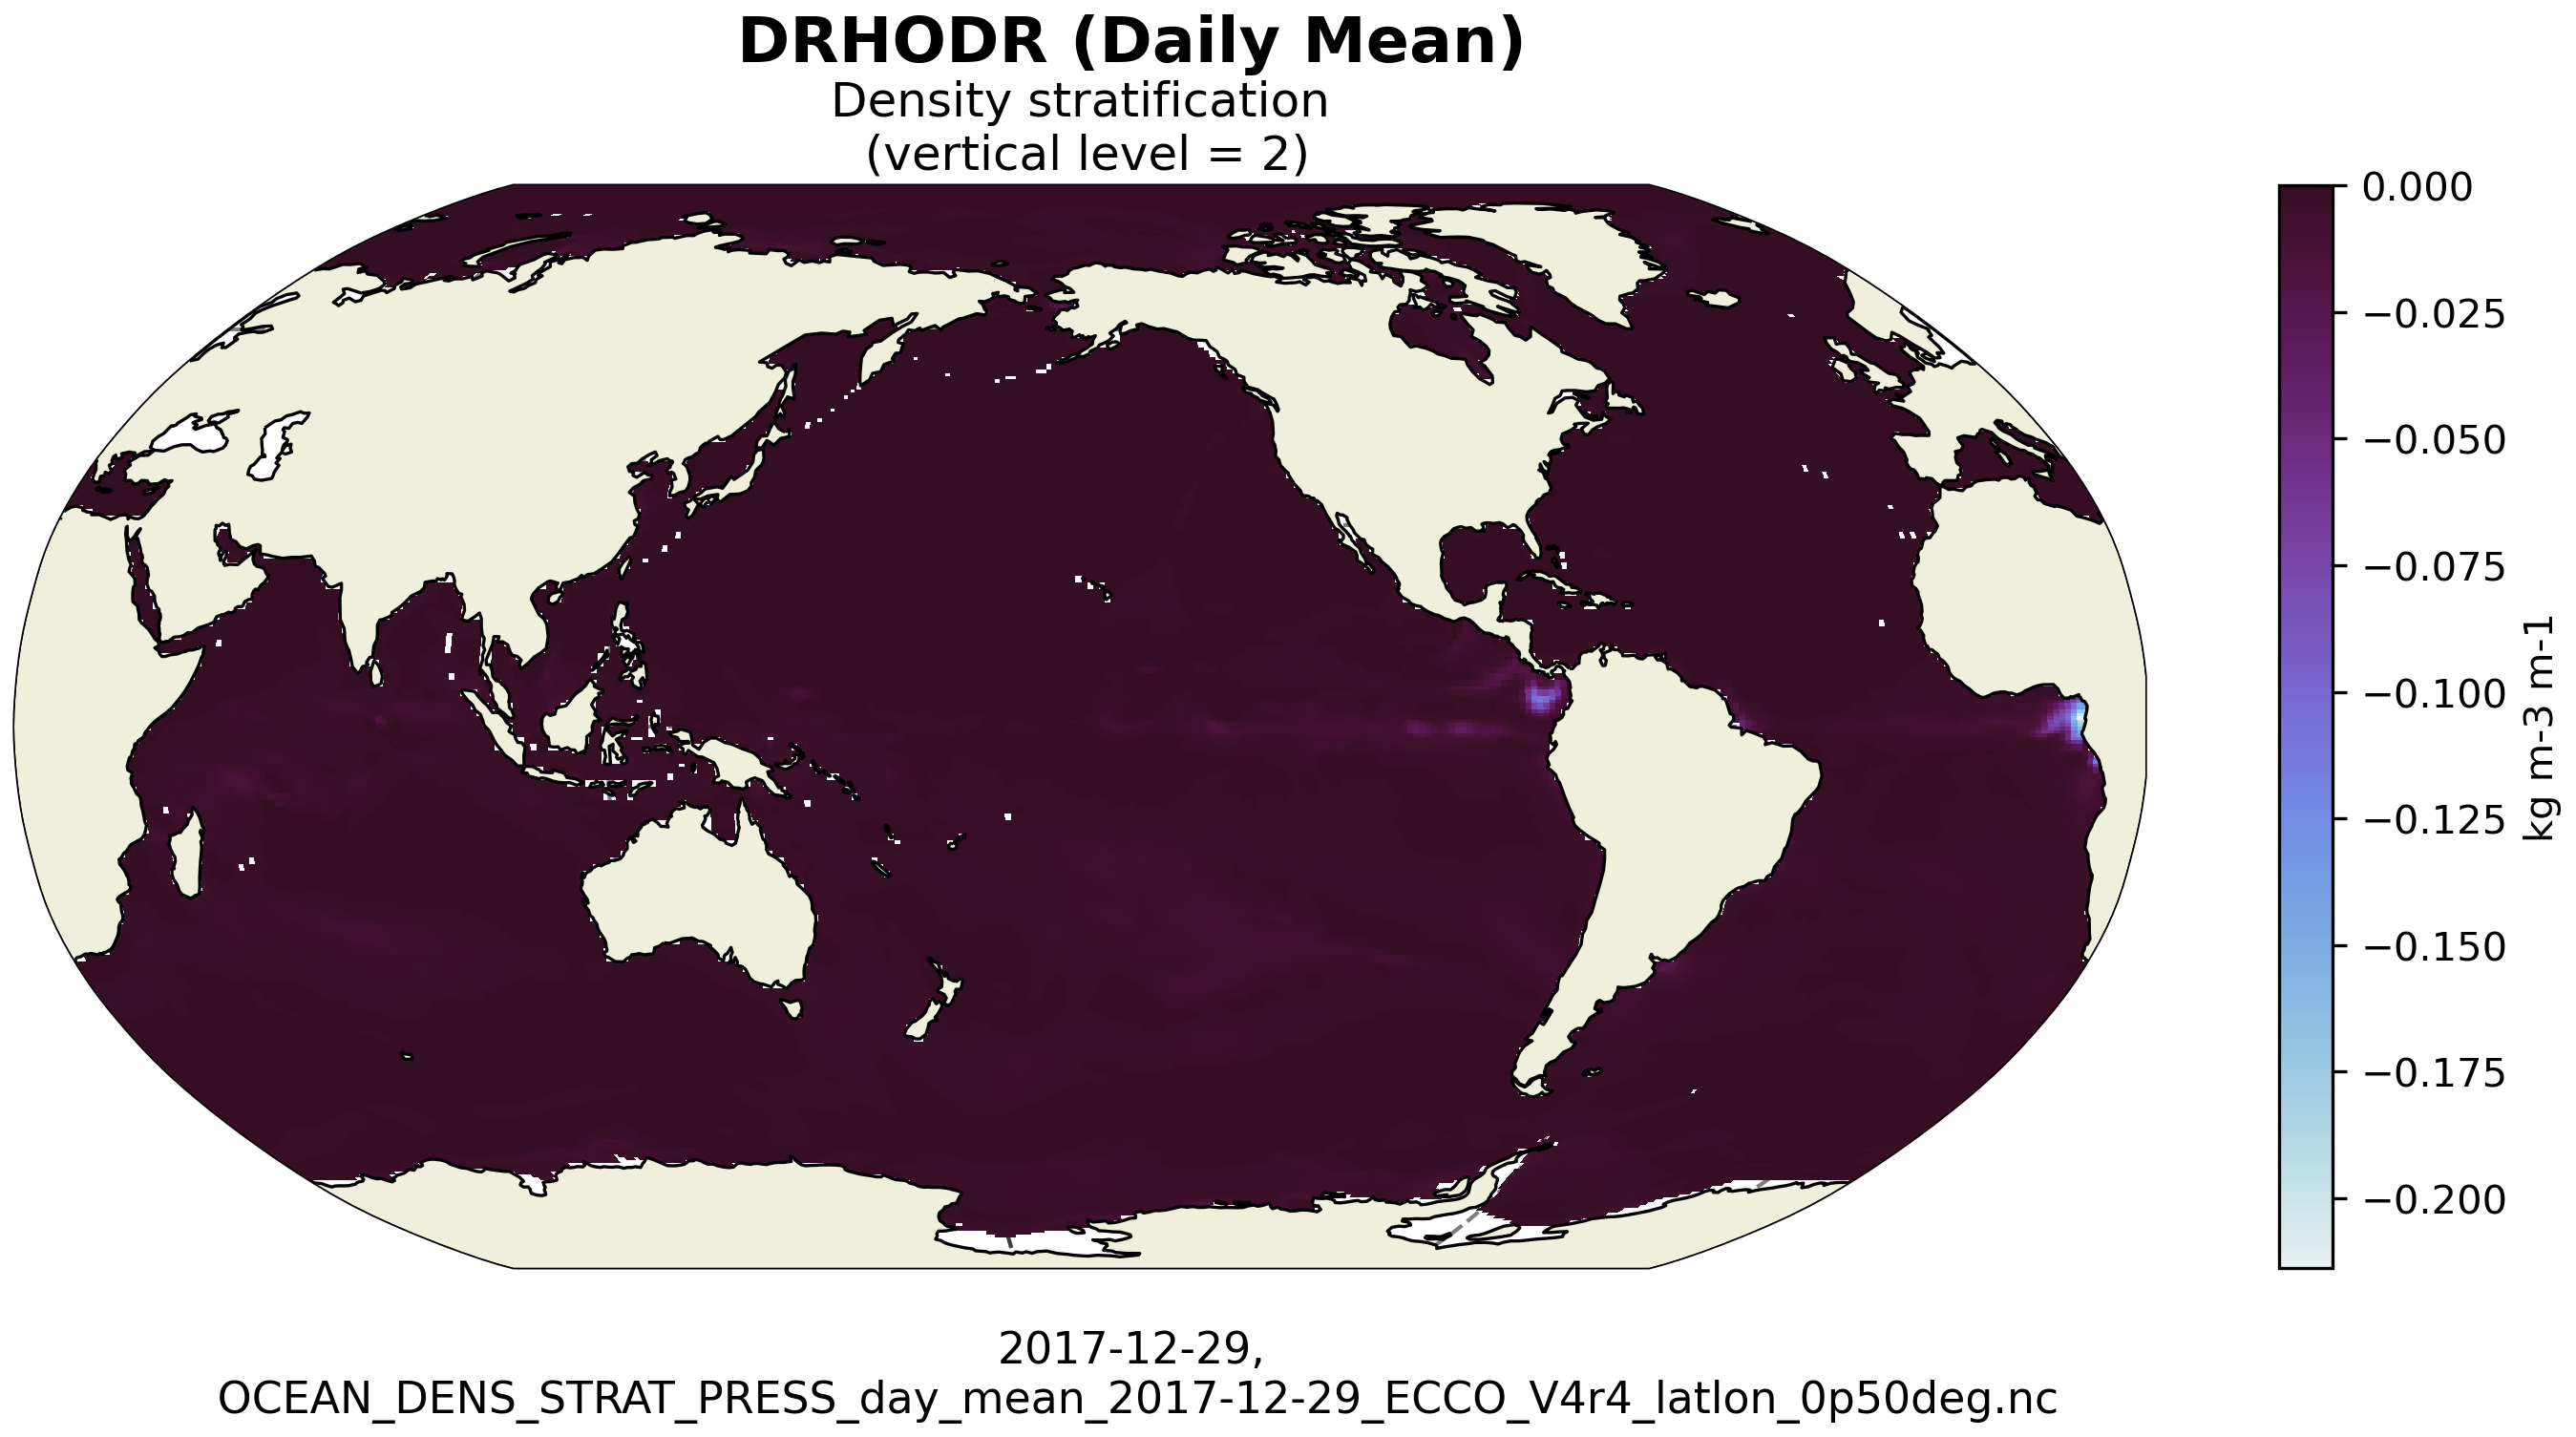
\includegraphics[scale=0.55]{../images/plots/v4r4/latlon_plots/Ocean_Density_Stratification_and_Hydrostatic_Pressure/DRHODR.png}
\caption{Dataset: OCEAN\_DENS\_STRAT\_PRESS, Variable: DRHODR}
\label{tab:table-OCEAN_DENS_STRAT_PRESS_DRHODR-Plot}
\end{figure}
\newpage
\pagebreak
\subsubsection{Latlon Variable: PHIHYD}
\begin{longtable}{|m{0.06\textwidth}|m{0.3\textwidth}|m{0.45\textwidth}|m{0.12\textwidth}|}
\caption{Attributes description of the variable 'PHIHYD' from OCEAN\_DENS\_STRAT\_PRESS's  dataset.}
\label{tab:table-OCEAN_DENS_STRAT_PRESS_PHIHYD} \\ 
\hline \endhead \hline \endfoot
\rowcolor{lightgray} \textbf{Storage Type} & \textbf{Variable Name} & \textbf{Description} & \textbf{Unit} \\ \hline
float32 & PHIHYD & Ocean hydrostatic pressure anomaly & m2 s-2 \\ \hline
\multicolumn{4}{|c|}{\cellcolor{lightgray}{\textbf{Description of the variable in Common Data language (CDL)}}} \\ \hline
\multicolumn{4}{|c|}{\fontfamily{lmtt}\selectfont{\makecell{\parbox{.95\textwidth}{\vspace*{0.25cm} \footnotesize{float32 PHIHYD(time, Z, latitude, longitude)\\
\hspace*{0.5cm}PHIHYD: \_FillValue = 9.96921e+36\\
\hspace*{0.5cm}PHIHYD: coordinates = time Z\\
\hspace*{0.5cm}PHIHYD: coverage\_content\_type = modelResult\\
\hspace*{0.5cm}PHIHYD: long\_name = Ocean hydrostatic pressure anomaly\\
\hspace*{0.5cm}PHIHYD: units = m2 s-2\\
\hspace*{0.5cm}PHIHYD: valid\_max = 783.9188232421875\\
\hspace*{0.5cm}PHIHYD: valid\_min = 74.71473693847656\\
}}}}} \\ \hline
\rowcolor{lightgray} \multicolumn{4}{|c|}{\textbf{Comments}} \\ \hline
\multicolumn{4}{|p{1\textwidth}|}{\footnotesize{{Phihyd = p(k) / rhoconst - g z*(k,t), where p = hydrostatic ocean pressure at depth level k, rhoconst = reference density (1029 kg m-3), g is acceleration due to gravity (9.81 m s-2), and z*(k,t) is model depth at level k and time t. units: p:[kg m-1 s-2], rhoconst:[kg m-3], g:[m s-2], h(t):[m]. note: includes atmospheric pressure loading. quantity referred to in some contexts as hydrostatic pressure anomaly. phibot accounts for the model's time-varying grid cell thickness (z* coordinate system). see phihydcr for hydrostatic pressure potential anomaly calculated using time-invariant grid cell thicknesses. phihyd is not corrected for global mean steric sea level changes related to density changes in the boussinesq volume-conserving model (greatbatch correction, see stergloh). }}} \\ \hline
\end{longtable}

\begin{figure}[H]
\centering
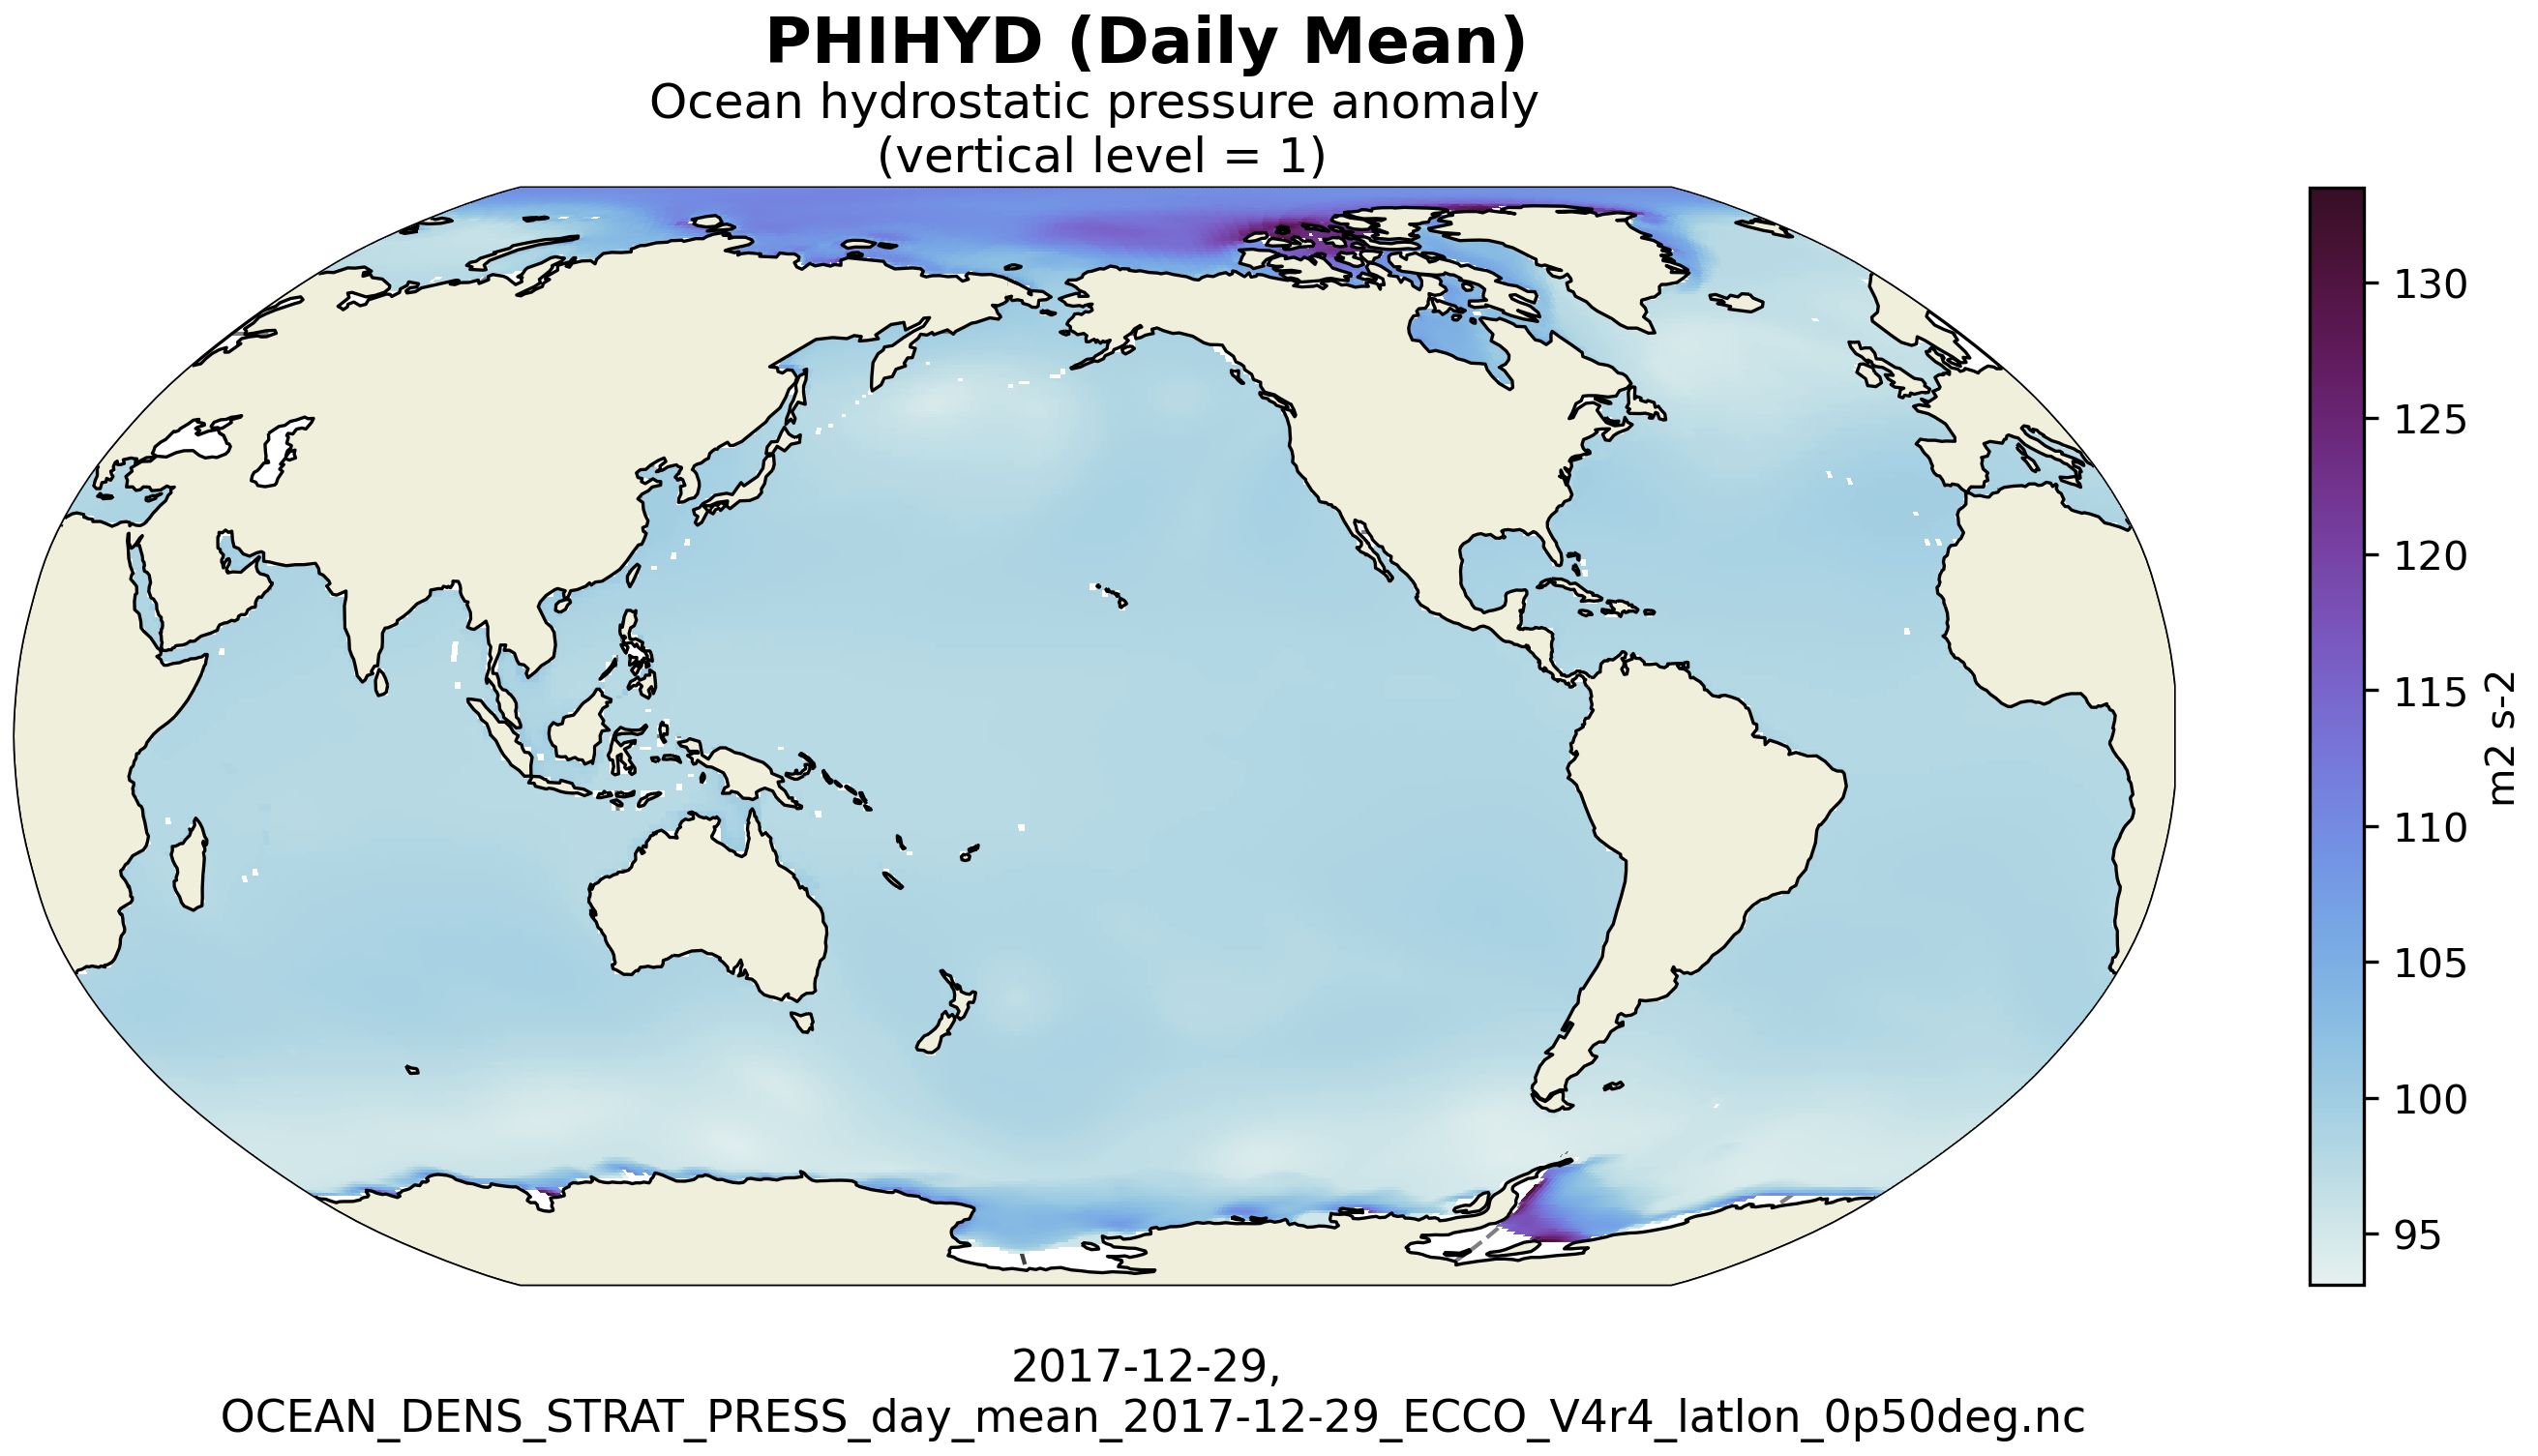
\includegraphics[scale=0.55]{../images/plots/v4r4/latlon_plots/Ocean_Density_Stratification_and_Hydrostatic_Pressure/PHIHYD.png}
\caption{Dataset: OCEAN\_DENS\_STRAT\_PRESS, Variable: PHIHYD}
\label{tab:table-OCEAN_DENS_STRAT_PRESS_PHIHYD-Plot}
\end{figure}
\newpage
\pagebreak
\subsubsection{Latlon Variable: RHOAnoma}
\begin{longtable}{|m{0.06\textwidth}|m{0.3\textwidth}|m{0.45\textwidth}|m{0.12\textwidth}|}
\caption{Attributes description of the variable 'RHOAnoma' from OCEAN\_DENS\_STRAT\_PRESS's  dataset.}
\label{tab:table-OCEAN_DENS_STRAT_PRESS_RHOAnoma} \\ 
\hline \endhead \hline \endfoot
\rowcolor{lightgray} \textbf{Storage Type} & \textbf{Variable Name} & \textbf{Description} & \textbf{Unit} \\ \hline
float32 & RHOAnoma & In-situ seawater density anomaly & kg m-3 \\ \hline
\multicolumn{4}{|c|}{\cellcolor{lightgray}{\textbf{Description of the variable in Common Data language (CDL)}}} \\ \hline
\multicolumn{4}{|c|}{\fontfamily{lmtt}\selectfont{\makecell{\parbox{.95\textwidth}{\vspace*{0.25cm} \footnotesize{float32 RHOAnoma(time, Z, latitude, longitude)\\
\hspace*{0.5cm}RHOAnoma: \_FillValue = 9.96921e+36\\
\hspace*{0.5cm}RHOAnoma: coordinates = time Z\\
\hspace*{0.5cm}RHOAnoma: coverage\_content\_type = modelResult\\
\hspace*{0.5cm}RHOAnoma: long\_name = In-situ seawater density anomaly\\
\hspace*{0.5cm}RHOAnoma: units = kg m-3\\
\hspace*{0.5cm}RHOAnoma: valid\_max = 25.540647506713867\\
\hspace*{0.5cm}RHOAnoma: valid\_min = -19.919862747192383\\
}}}}} \\ \hline
\rowcolor{lightgray} \multicolumn{4}{|c|}{\textbf{Comments}} \\ \hline
\multicolumn{4}{|p{1\textwidth}|}{\footnotesize{{In-situ seawater density anomaly relative to the reference density, rhoconst. rhoconst = 1029 kg m-3}}} \\ \hline
\end{longtable}

\begin{figure}[H]
\centering
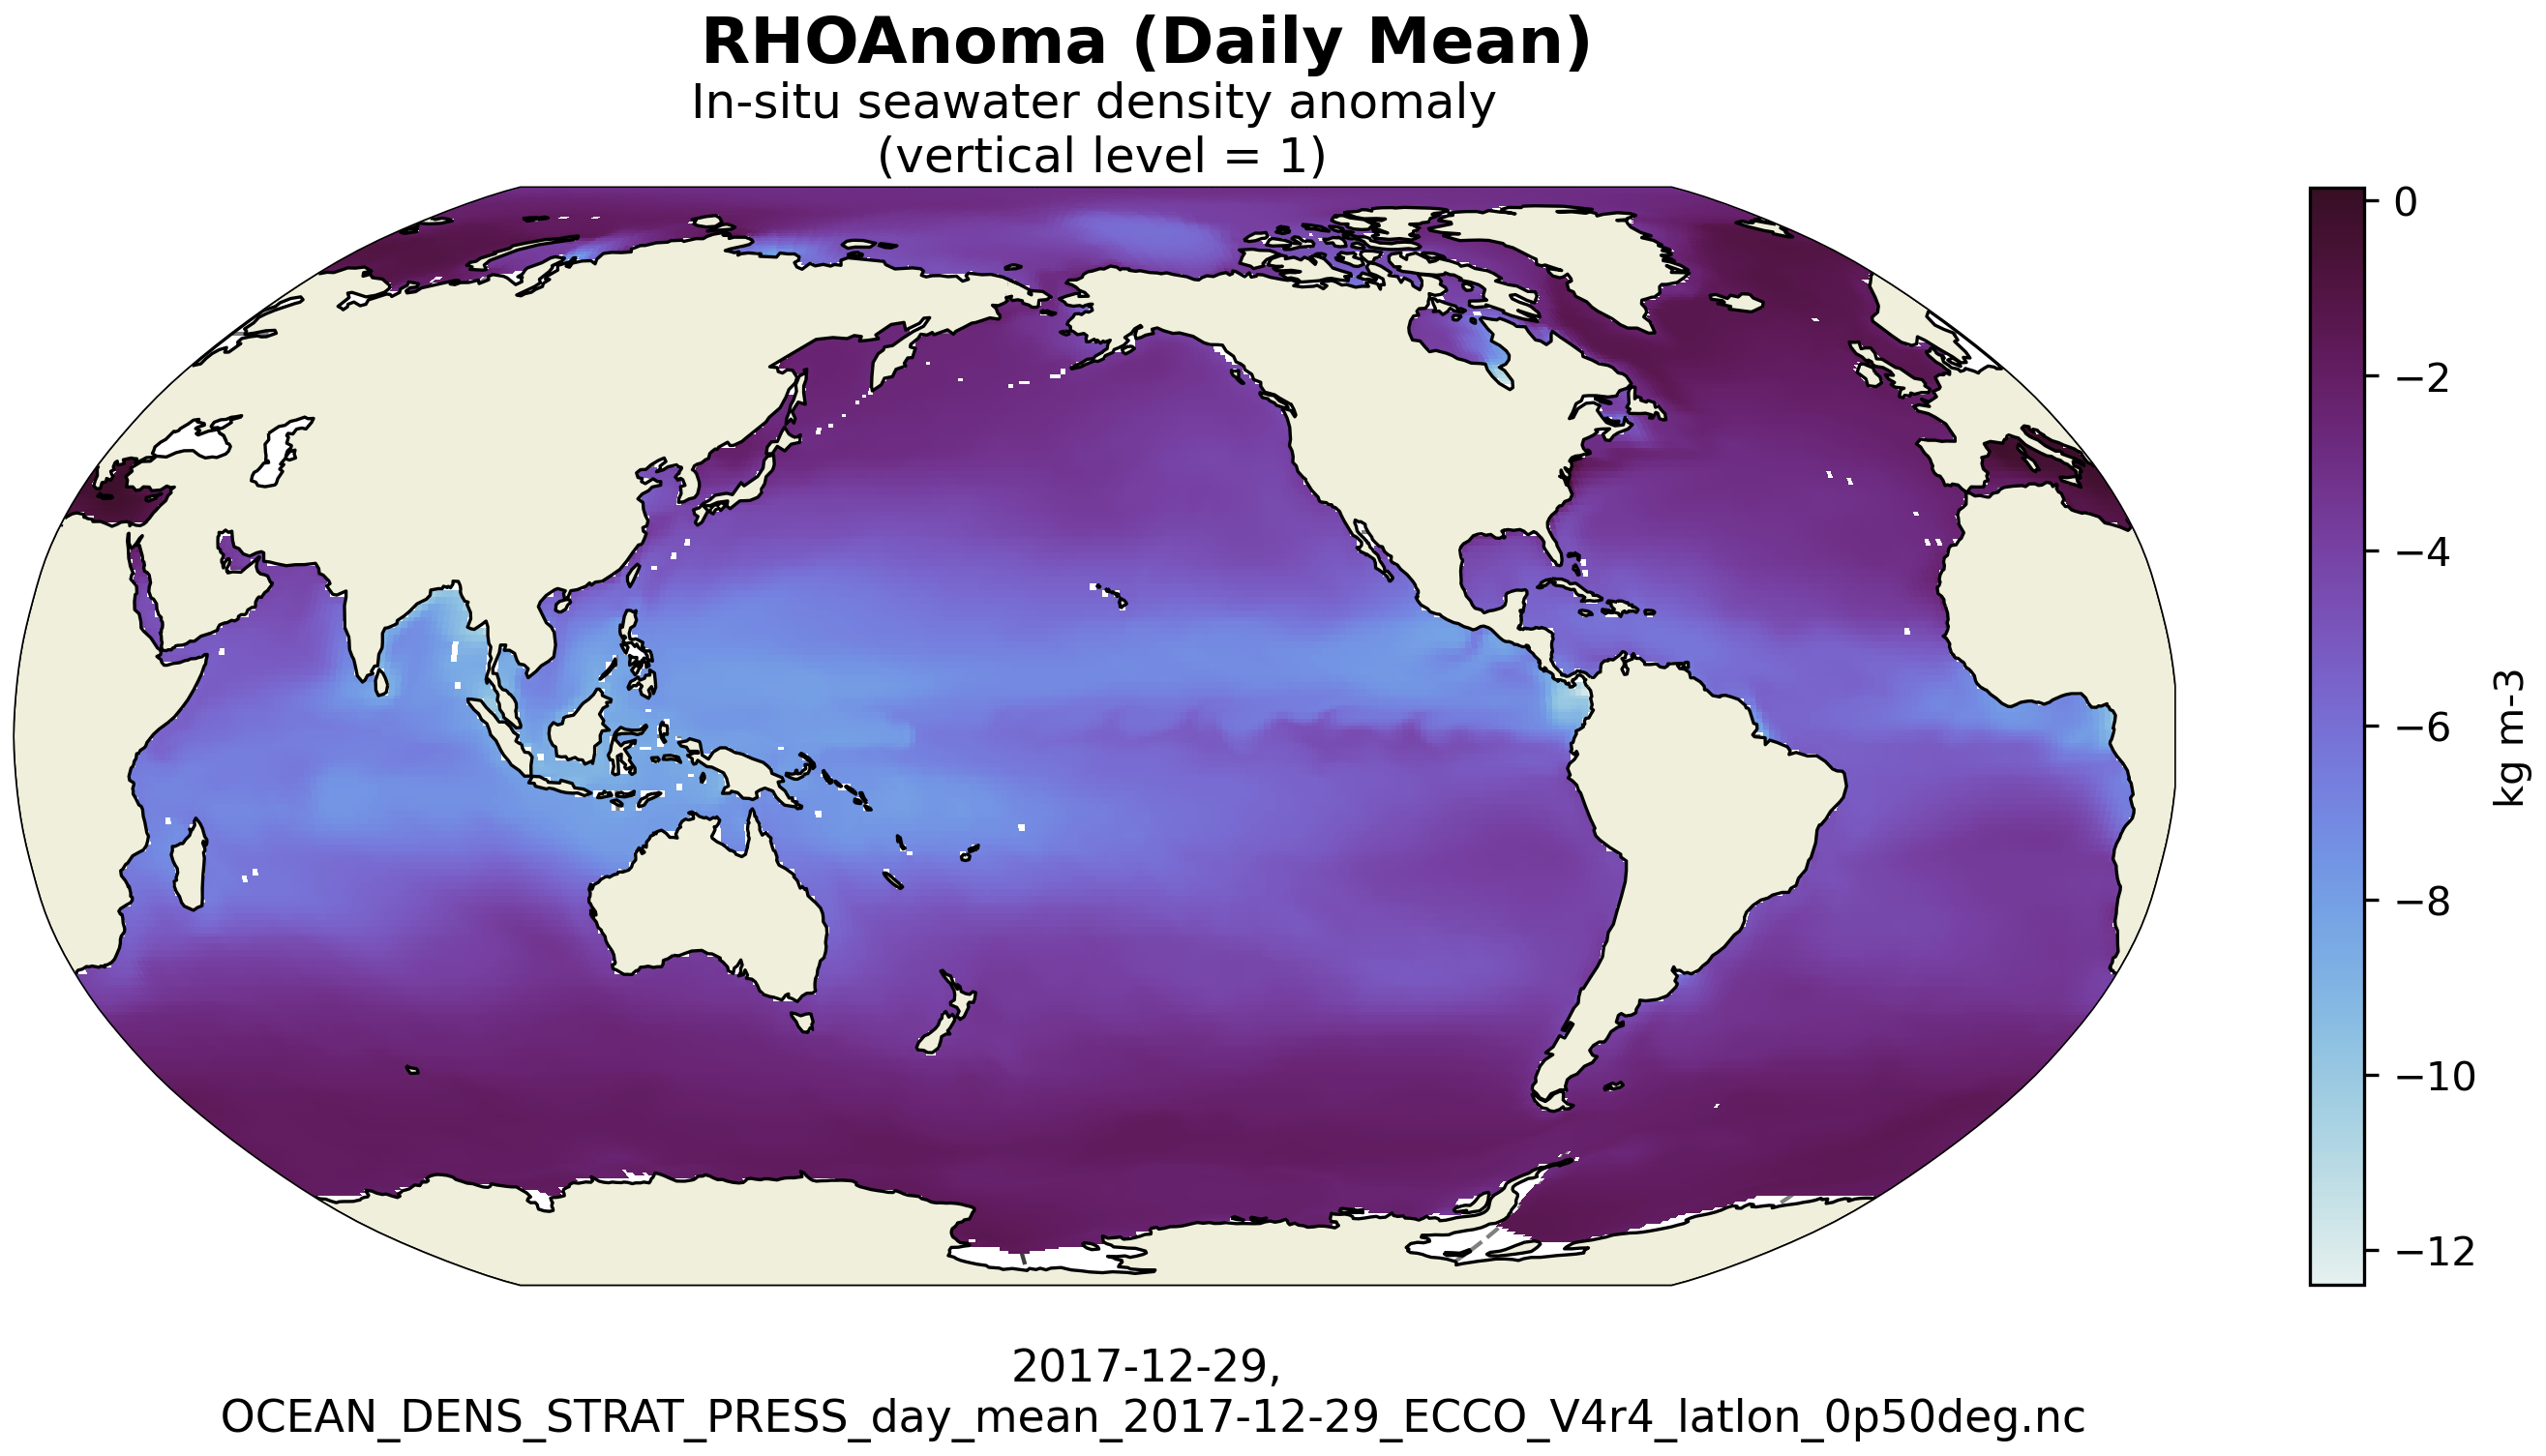
\includegraphics[scale=0.55]{../images/plots/v4r4/latlon_plots/Ocean_Density_Stratification_and_Hydrostatic_Pressure/RHOAnoma.png}
\caption{Dataset: OCEAN\_DENS\_STRAT\_PRESS, Variable: RHOAnoma}
\label{tab:table-OCEAN_DENS_STRAT_PRESS_RHOAnoma-Plot}
\end{figure}
\newpage
\subsection{Latlon dataset of OCEAN\_MIXED\_LAYER\_DEPTH}
\newp
\subsubsection{Overview}
This dataset provides 2D fileds of ocean mixed layer depth interpolated to a regular 0.5-degree grid from the ECCO Version 4 Release 4 (V4r4) ocean and sea-ice state estimate. The dataset is provided on daily-average and monthly-average time resolution. 
\begin{longtable}{|m{0.15\textwidth}|m{0.64\textwidth}|m{0.12\textwidth}|}
\caption{Coordinates and Variables in the dataset OCEAN\_MIXED\_LAYER\_DEPTH}
\label{tab:table-OCEAN_MIXED_LAYER_DEPTH-fields} \\ 
\hline \endhead \hline \endfoot
\rowcolor{lightgray} \multicolumn{1}{|c|}{\textbf{Coordinates}} & \multicolumn{1}{|c|}{\textbf{Description of data coordinates}} &  \multicolumn{1}{|c|}{\textbf{Unit}}\\ \hline
time &Center time of averaging period &--none--  \\ \hline
latitude &Latitude at grid cell center &degrees\_north  \\ \hline
longitude &Longitude at grid cell center &degrees\_east  \\ \hline
time\_bnds &Time bounds of averaging period &--none--  \\ \hline
latitude\_bnds &Latitude bounds grid cells &--none--  \\ \hline
longitude\_bnds &Longitude bounds grid cells &--none--  \\ \hline
\rowcolor{lightgray} \multicolumn{1}{|c|}{\textbf{Variables}} & \multicolumn{1}{|c|}{\textbf{Description of data variables}} &  \multicolumn{1}{|c|}{\textbf{Unit}}\\ \hline
MXLDEPTH &Mixed-layer depth diagnosed using the temperature difference criterion of kara et al., 2000 &m  \\ \hline
\end{longtable}

\newp
\pagebreak
\subsubsection{Latlon Variable: MXLDEPTH}
\begin{longtable}{|m{0.06\textwidth}|m{0.3\textwidth}|m{0.45\textwidth}|m{0.12\textwidth}|}
\caption{Attributes description of the variable 'MXLDEPTH' from OCEAN\_MIXED\_LAYER\_DEPTH's  dataset.}
\label{tab:table-OCEAN_MIXED_LAYER_DEPTH_MXLDEPTH} \\ 
\hline \endhead \hline \endfoot
\rowcolor{lightgray} \textbf{Storage Type} & \textbf{Variable Name} & \textbf{Description} & \textbf{Unit} \\ \hline
float32 & MXLDEPTH & Mixed-layer depth diagnosed using the temperature difference criterion of kara et al., 2000 & m \\ \hline
\multicolumn{4}{|c|}{\cellcolor{lightgray}{\textbf{Description of the variable in Common Data language (CDL)}}} \\ \hline
\multicolumn{4}{|c|}{\fontfamily{lmtt}\selectfont{\makecell{\parbox{.95\textwidth}{\vspace*{0.25cm} \footnotesize{float32 MXLDEPTH(time, latitude, longitude)\\
\hspace*{0.5cm}MXLDEPTH: \_FillValue = 9.96921e+36\\
\hspace*{0.5cm}MXLDEPTH: coordinates = time\\
\hspace*{0.5cm}MXLDEPTH: coverage\_content\_type = modelResult\\
\hspace*{0.5cm}MXLDEPTH: long\_name = Mixed-layer depth diagnosed using the temperature difference criterion of Kara et al., 2000\\
\hspace*{0.5cm}MXLDEPTH: standard\_name = ocean mixed layer thickness\\
\hspace*{0.5cm}MXLDEPTH: units = m\\
\hspace*{0.5cm}MXLDEPTH: valid\_max = 5331.2001953125\\
\hspace*{0.5cm}MXLDEPTH: valid\_min = 5.000001430511475\\
}}}}} \\ \hline
\rowcolor{lightgray} \multicolumn{4}{|c|}{\textbf{Comments}} \\ \hline
\multicolumn{4}{|p{1\textwidth}|}{\footnotesize{{Mixed-layer depth as determined by the depth where waters are first 0.8 degrees celsius colder than the surface. see kara et al. (jgr, 2000). . note: the kara et al. criterion may not be appropriate for some applications. if needed, mixed layer depth can be calculated using different criteria. see vertical density stratification (drhodr) and density anomaly (rhoanoma).}}} \\ \hline
\end{longtable}

\begin{figure}[H]
\centering
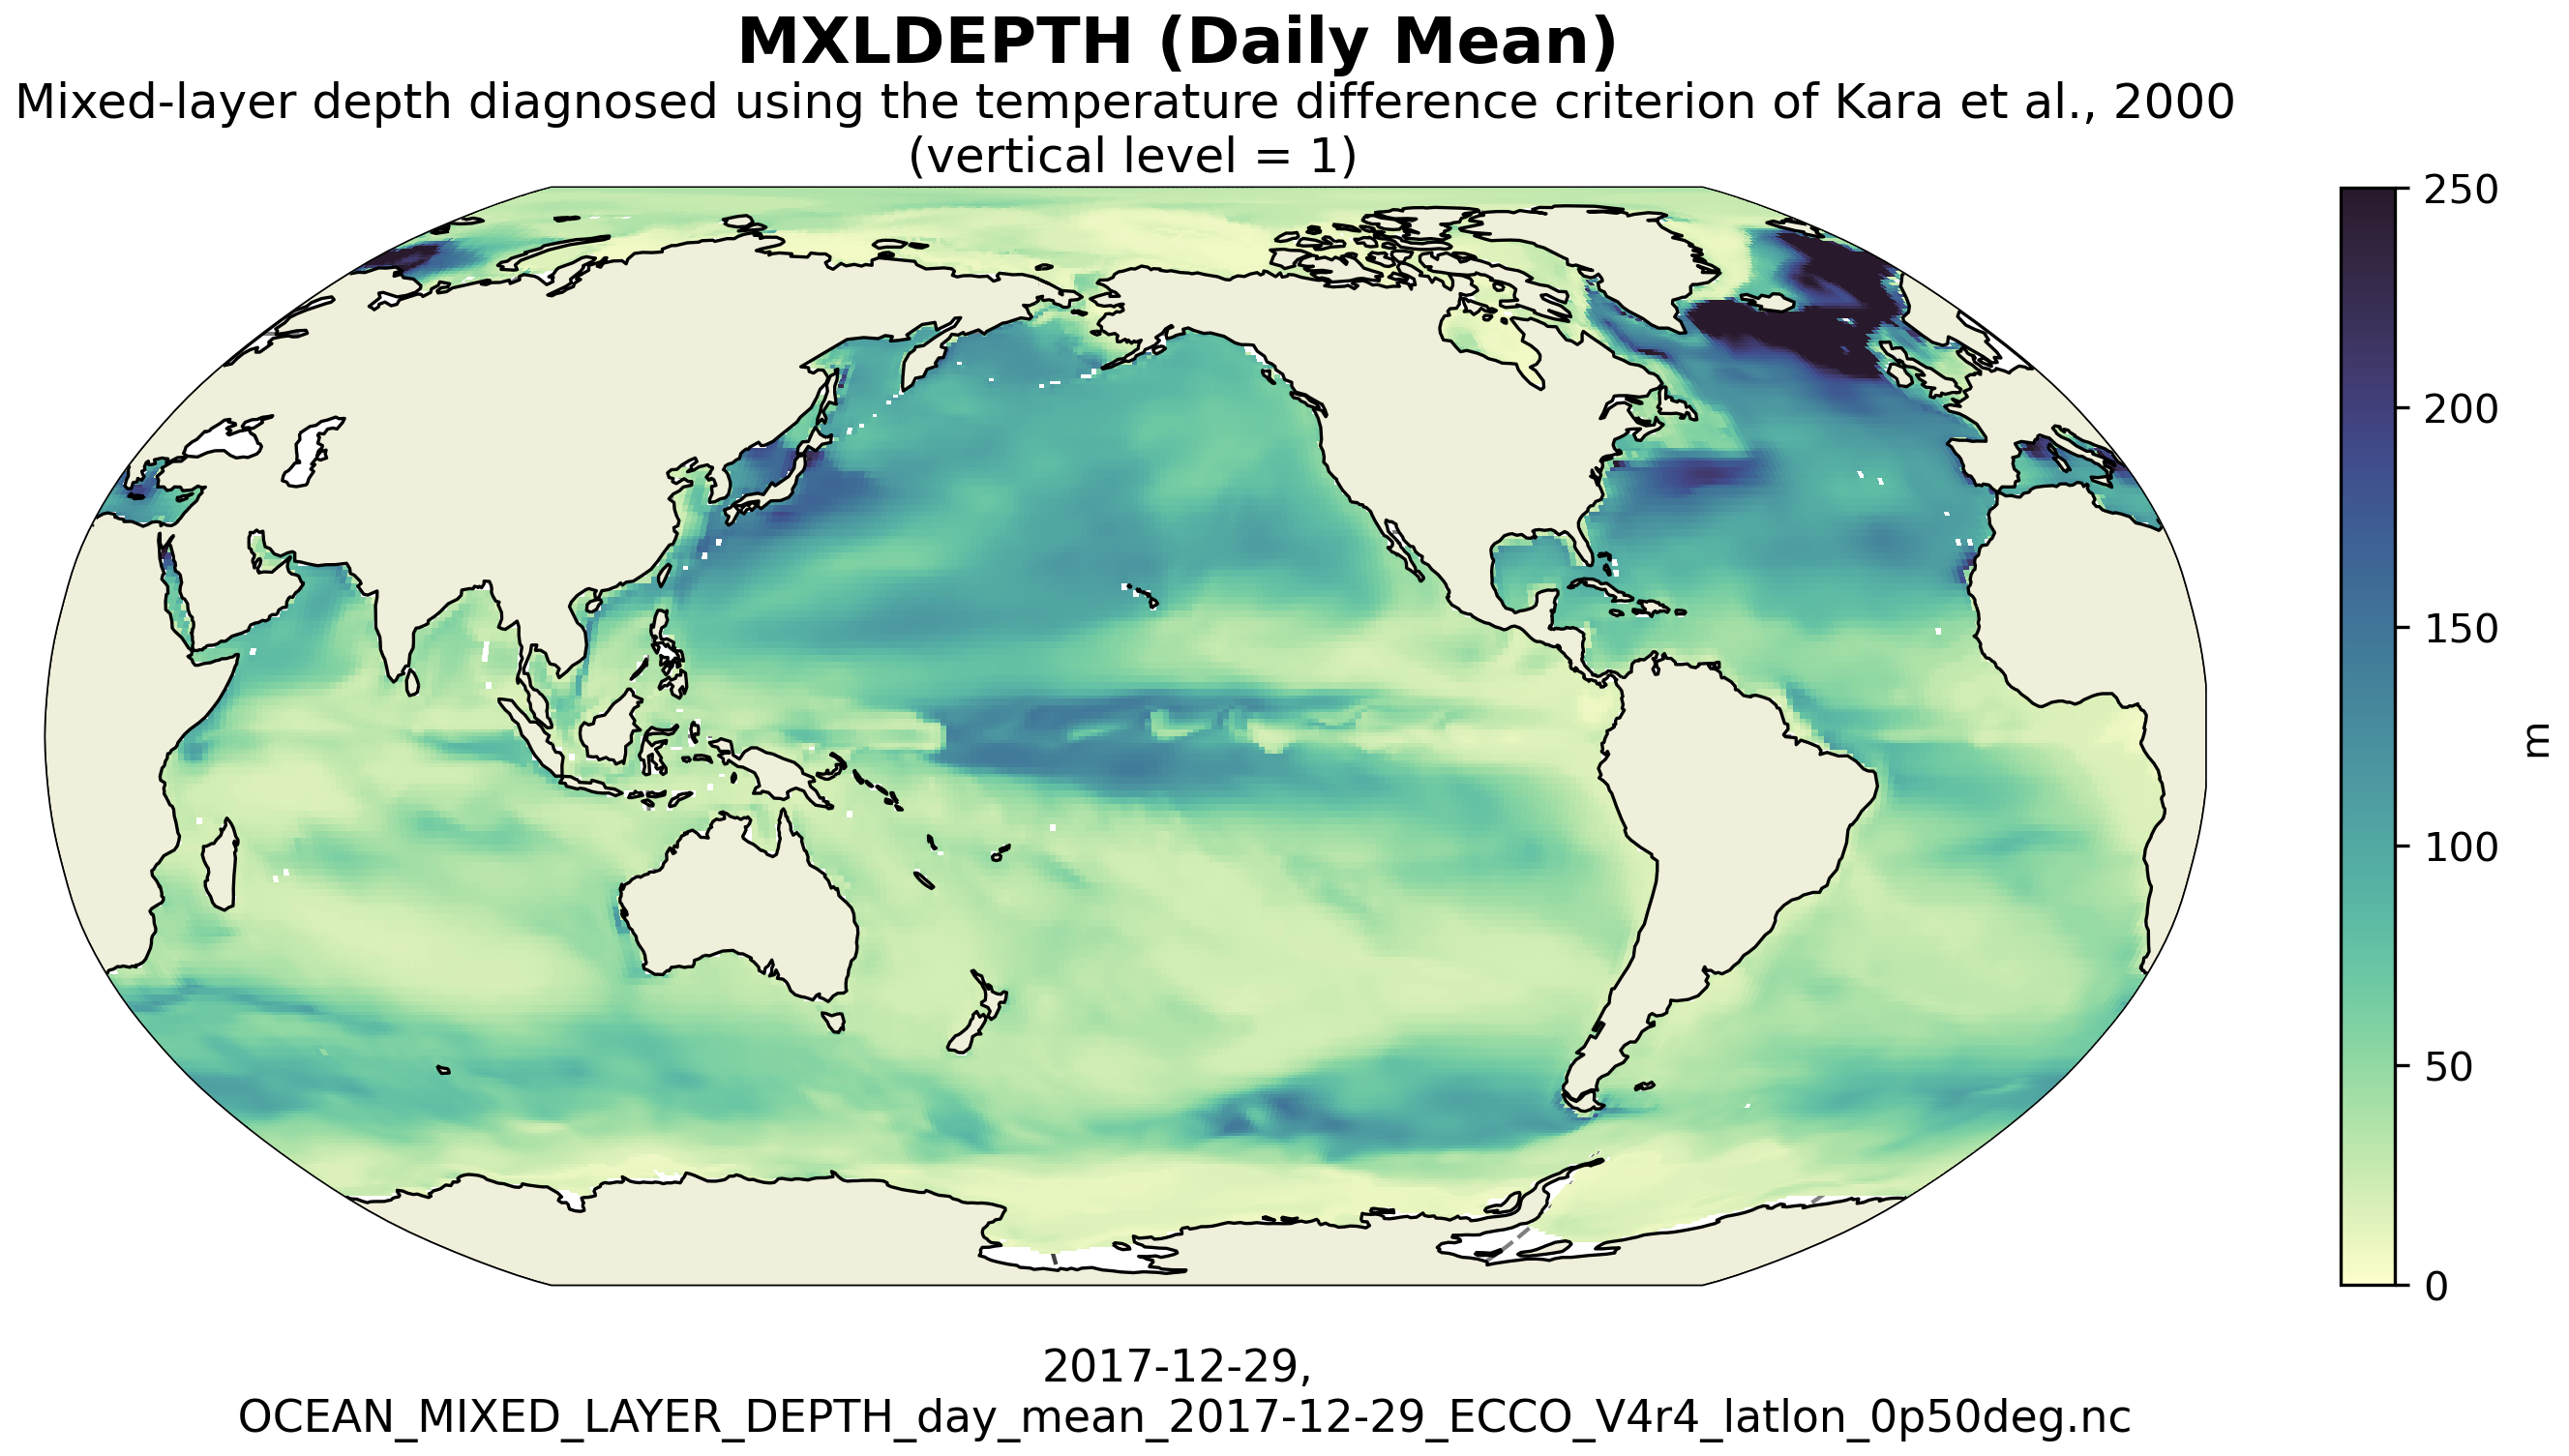
\includegraphics[scale=0.55]{../images/plots/v4r4/latlon_plots/Ocean_Mixed_Layer_Depth/MXLDEPTH.png}
\caption{Dataset: OCEAN\_MIXED\_LAYER\_DEPTH, Variable: MXLDEPTH}
\label{tab:table-OCEAN_MIXED_LAYER_DEPTH_MXLDEPTH-Plot}
\end{figure}
\newpage
\subsection{Latlon dataset of OCEAN\_TEMPERATURE\_SALINITY}
\newp
\subsubsection{Overview}
This dataset provides 3D fields of ocean potential temperature and salinity interpolated to a regular 0.5-degree grid from the ECCO Version 4 Release 4 (V4r4) ocean and sea-ice state estimate. The dataset is provided on daily-average and monthly-average time resolution. 
\begin{longtable}{|m{0.15\textwidth}|m{0.64\textwidth}|m{0.12\textwidth}|}
\caption{Coordinates and Variables in the dataset OCEAN\_TEMPERATURE\_SALINITY}
\label{tab:table-OCEAN_TEMPERATURE_SALINITY-fields} \\ 
\hline \endhead \hline \endfoot
\rowcolor{lightgray} \multicolumn{1}{|c|}{\textbf{Coordinates}} & \multicolumn{1}{|c|}{\textbf{Description of data coordinates}} &  \multicolumn{1}{|c|}{\textbf{Unit}}\\ \hline
time &Center time of averaging period &--none--  \\ \hline
Z &Depth of grid cell center &m  \\ \hline
latitude &Latitude at grid cell center &degrees\_north  \\ \hline
longitude &Longitude at grid cell center &degrees\_east  \\ \hline
time\_bnds &Time bounds of averaging period &--none--  \\ \hline
latitude\_bnds &Latitude bounds grid cells &--none--  \\ \hline
longitude\_bnds &Longitude bounds grid cells &--none--  \\ \hline
Z\_bnds &Depths of grid cell upper and lower interfaces &--none--  \\ \hline
\rowcolor{lightgray} \multicolumn{1}{|c|}{\textbf{Variables}} & \multicolumn{1}{|c|}{\textbf{Description of data variables}} &  \multicolumn{1}{|c|}{\textbf{Unit}}\\ \hline
THETA &Potential temperature  &degree\_C  \\ \hline
SALT &Salinity &1e-3  \\ \hline
\end{longtable}

\newp
\pagebreak
\subsubsection{Latlon Variable: SALT}
\begin{longtable}{|m{0.06\textwidth}|m{0.3\textwidth}|m{0.45\textwidth}|m{0.12\textwidth}|}
\caption{Attributes description of the variable 'SALT' from OCEAN\_TEMPERATURE\_SALINITY's  dataset.}
\label{tab:table-OCEAN_TEMPERATURE_SALINITY_SALT} \\ 
\hline \endhead \hline \endfoot
\rowcolor{lightgray} \textbf{Storage Type} & \textbf{Variable Name} & \textbf{Description} & \textbf{Unit} \\ \hline
float32 & SALT & Salinity & 1e-3 \\ \hline
\multicolumn{4}{|c|}{\cellcolor{lightgray}{\textbf{Description of the variable in Common Data language (CDL)}}} \\ \hline
\multicolumn{4}{|c|}{\fontfamily{lmtt}\selectfont{\makecell{\parbox{.95\textwidth}{\vspace*{0.25cm} \footnotesize{float32 SALT(time, Z, latitude, longitude)\\
\hspace*{0.5cm}SALT: \_FillValue = 9.96921e+36\\
\hspace*{0.5cm}SALT: coordinates = time Z\\
\hspace*{0.5cm}SALT: coverage\_content\_type = modelResult\\
\hspace*{0.5cm}SALT: long\_name = Salinity\\
\hspace*{0.5cm}SALT: standard\_name = sea water salinity\\
\hspace*{0.5cm}SALT: units = 1e-3\\
\hspace*{0.5cm}SALT: valid\_max = 41.321231842041016\\
\hspace*{0.5cm}SALT: valid\_min = 16.73577880859375\\
}}}}} \\ \hline
\rowcolor{lightgray} \multicolumn{4}{|c|}{\textbf{Comments}} \\ \hline
\multicolumn{4}{|p{1\textwidth}|}{\footnotesize{{Defined using cf convention 'sea water salinity is the salt content of sea water, often on the practical salinity scale of 1978. however, the unqualified term 'salinity' is generic and does not necessarily imply any particular method of calculation. the units of salinity are dimensionless and the units attribute should normally be given as 1e-3 or 0.001 i.e. parts per thousand.' see https://cfconventions.org/data/cf-standard-names/73/build/cf-standard-name-table.html}}} \\ \hline
\end{longtable}

\begin{figure}[H]
\centering
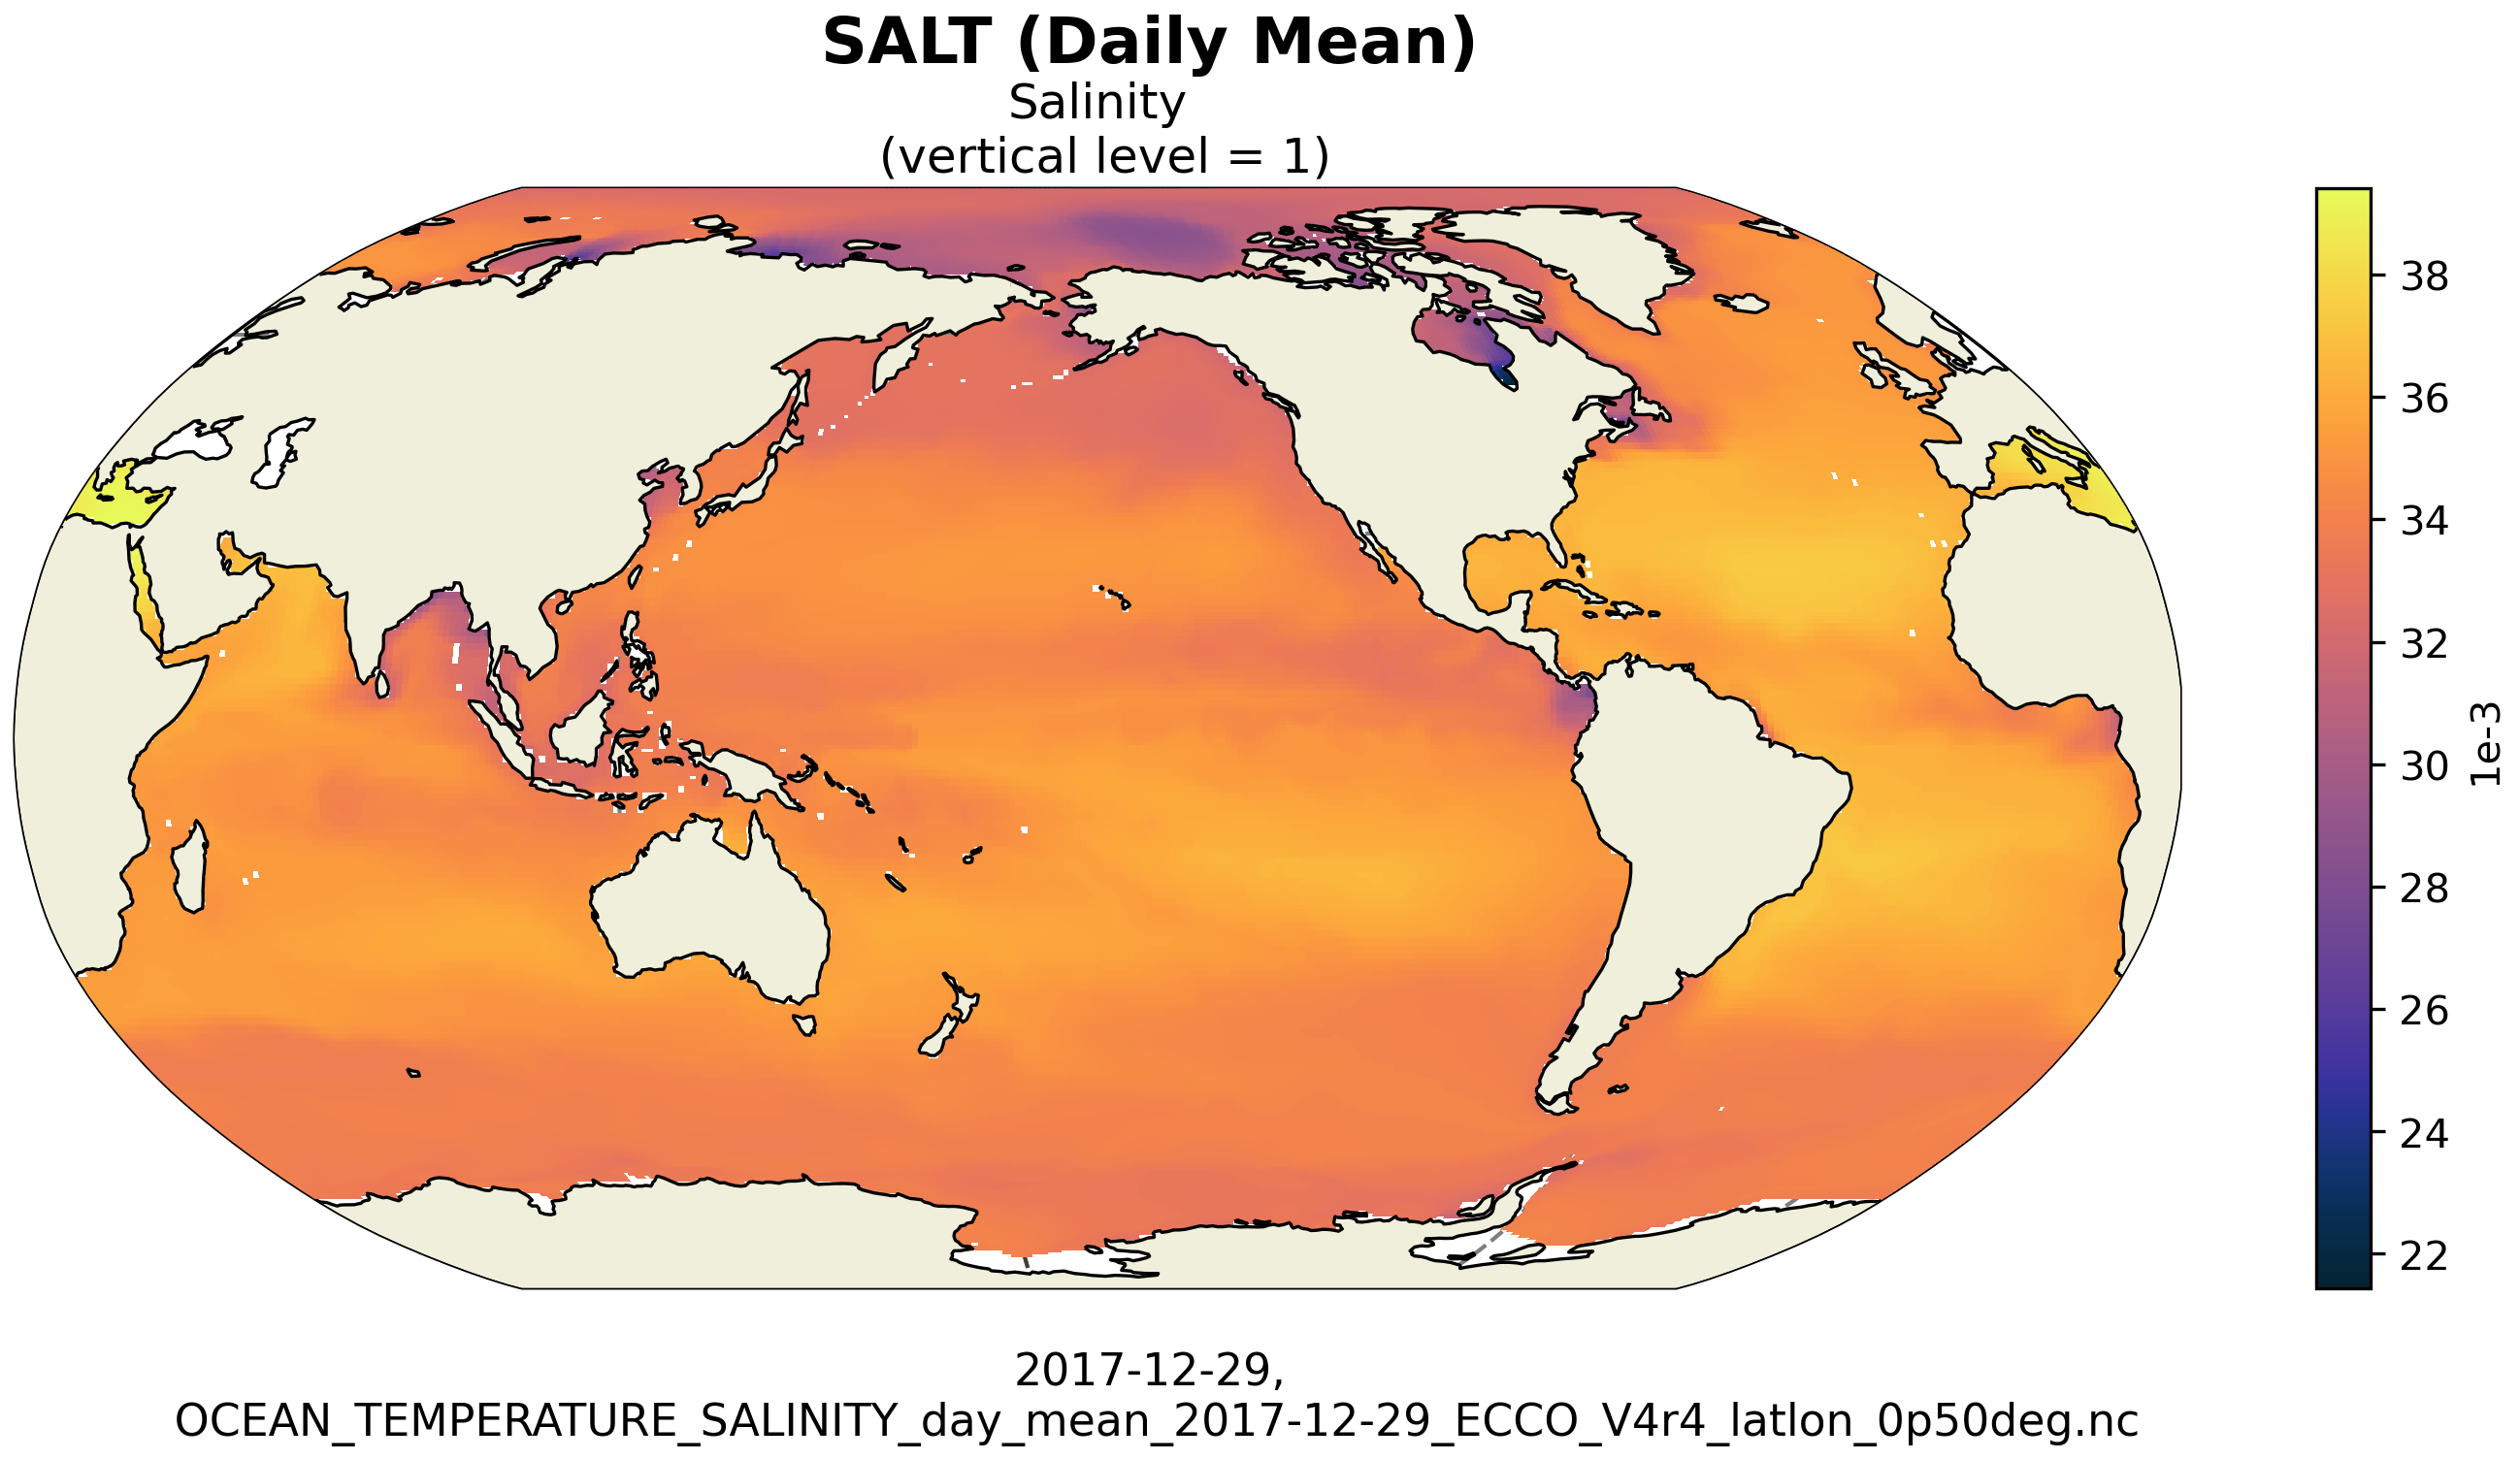
\includegraphics[scale=0.55]{../images/plots/v4r4/latlon_plots/Ocean_Temperature_and_Salinity/SALT.png}
\caption{Dataset: OCEAN\_TEMPERATURE\_SALINITY, Variable: SALT}
\label{tab:table-OCEAN_TEMPERATURE_SALINITY_SALT-Plot}
\end{figure}
\newpage
\pagebreak
\subsubsection{Latlon Variable: THETA}
\begin{longtable}{|m{0.06\textwidth}|m{0.3\textwidth}|m{0.45\textwidth}|m{0.12\textwidth}|}
\caption{Attributes description of the variable 'THETA' from OCEAN\_TEMPERATURE\_SALINITY's  dataset.}
\label{tab:table-OCEAN_TEMPERATURE_SALINITY_THETA} \\ 
\hline \endhead \hline \endfoot
\rowcolor{lightgray} \textbf{Storage Type} & \textbf{Variable Name} & \textbf{Description} & \textbf{Unit} \\ \hline
float32 & THETA & Potential temperature  & degree\_C \\ \hline
\multicolumn{4}{|c|}{\cellcolor{lightgray}{\textbf{Description of the variable in Common Data language (CDL)}}} \\ \hline
\multicolumn{4}{|c|}{\fontfamily{lmtt}\selectfont{\makecell{\parbox{.95\textwidth}{\vspace*{0.25cm} \footnotesize{float32 THETA(time, Z, latitude, longitude)\\
\hspace*{0.5cm}THETA: \_FillValue = 9.96921e+36\\
\hspace*{0.5cm}THETA: coordinates = time Z\\
\hspace*{0.5cm}THETA: coverage\_content\_type = modelResult\\
\hspace*{0.5cm}THETA: long\_name = Potential temperature \\
\hspace*{0.5cm}THETA: standard\_name = sea water potential temperature\\
\hspace*{0.5cm}THETA: units = degree C\\
\hspace*{0.5cm}THETA: valid\_max = 36.425140380859375\\
\hspace*{0.5cm}THETA: valid\_min = -2.9179372787475586\\
}}}}} \\ \hline
\rowcolor{lightgray} \multicolumn{4}{|c|}{\textbf{Comments}} \\ \hline
\multicolumn{4}{|p{1\textwidth}|}{\footnotesize{{Sea water potential temperature is the temperature a parcel of sea water would have if moved adiabatically to sea level pressure. note: the equation of state is a modified unesco formula by jackett and mcdougall (1995), which uses the model variable potential temperature as input assuming a horizontally and temporally constant pressure of \$p\_0=-g 
ho\_\{0\} z\$.}}} \\ \hline
\end{longtable}

\begin{figure}[H]
\centering
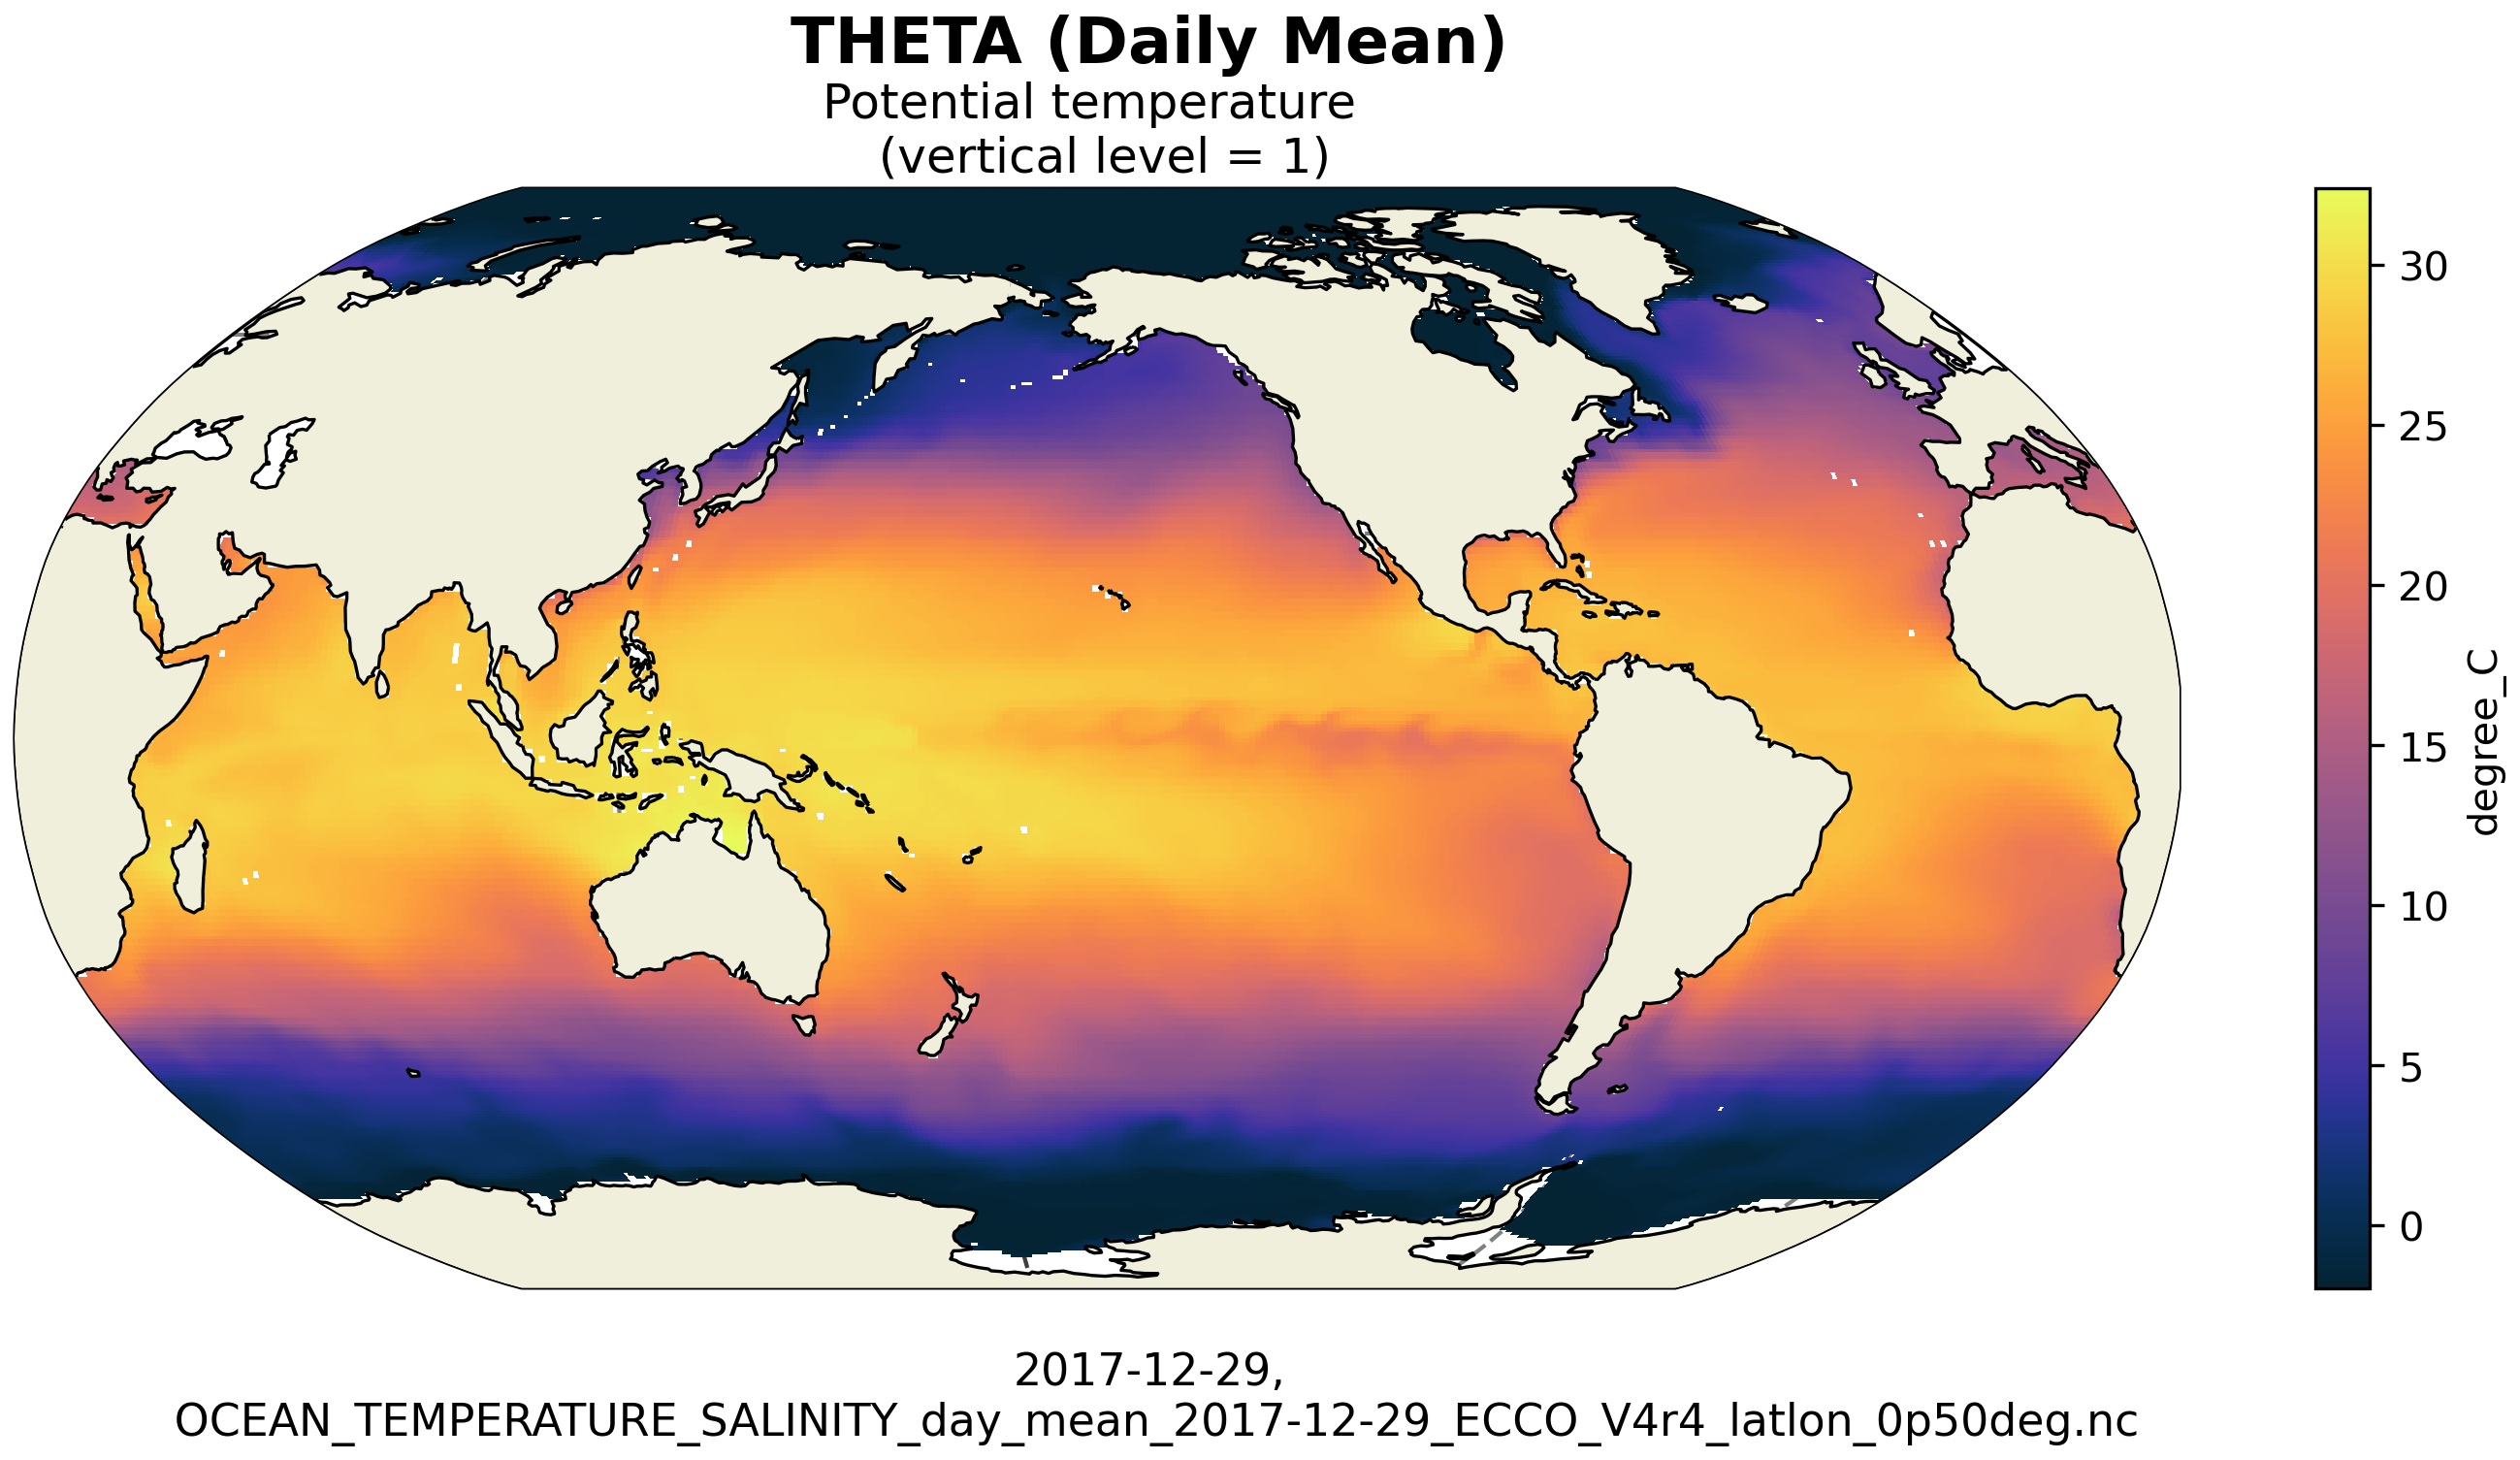
\includegraphics[scale=0.55]{../images/plots/v4r4/latlon_plots/Ocean_Temperature_and_Salinity/THETA.png}
\caption{Dataset: OCEAN\_TEMPERATURE\_SALINITY, Variable: THETA}
\label{tab:table-OCEAN_TEMPERATURE_SALINITY_THETA-Plot}
\end{figure}
\newpage
\subsection{Latlon dataset of OCEAN\_VELOCITY}
\newp
\subsubsection{Overview}
This dataset provides 3D fields of ocean velocity interpolated to a regular 0.5-degree grid from the ECCO Version 4 Release 4 (V4r4) ocean and sea-ice state estimate. The dataset is provided on daily-average and monthly-average time resolution. 
\begin{longtable}{|m{0.15\textwidth}|m{0.64\textwidth}|m{0.12\textwidth}|}
\caption{Coordinates and Variables in the dataset OCEAN\_VELOCITY}
\label{tab:table-OCEAN_VELOCITY-fields} \\ 
\hline \endhead \hline \endfoot
\rowcolor{lightgray} \multicolumn{1}{|c|}{\textbf{Coordinates}} & \multicolumn{1}{|c|}{\textbf{Description of data coordinates}} &  \multicolumn{1}{|c|}{\textbf{Unit}}\\ \hline
time &Center time of averaging period &--none--  \\ \hline
Z &Depth of grid cell center &m  \\ \hline
latitude &Latitude at grid cell center &degrees\_north  \\ \hline
longitude &Longitude at grid cell center &degrees\_east  \\ \hline
time\_bnds &Time bounds of averaging period &--none--  \\ \hline
latitude\_bnds &Latitude bounds grid cells &--none--  \\ \hline
longitude\_bnds &Longitude bounds grid cells &--none--  \\ \hline
Z\_bnds &Depths of grid cell upper and lower interfaces &--none--  \\ \hline
\rowcolor{lightgray} \multicolumn{1}{|c|}{\textbf{Variables}} & \multicolumn{1}{|c|}{\textbf{Description of data variables}} &  \multicolumn{1}{|c|}{\textbf{Unit}}\\ \hline
EVEL &Zonal (east-west) velocity &m s-1  \\ \hline
NVEL &Meridional (north-south) velocity &m s-1  \\ \hline
WVEL &Vertical velocity &m s-1  \\ \hline
\end{longtable}

\newp
\pagebreak
\subsubsection{Latlon Variable: EVEL}
\begin{longtable}{|m{0.06\textwidth}|m{0.3\textwidth}|m{0.45\textwidth}|m{0.12\textwidth}|}
\caption{Attributes description of the variable 'EVEL' from OCEAN\_VELOCITY's  dataset.}
\label{tab:table-OCEAN_VELOCITY_EVEL} \\ 
\hline \endhead \hline \endfoot
\rowcolor{lightgray} \textbf{Storage Type} & \textbf{Variable Name} & \textbf{Description} & \textbf{Unit} \\ \hline
float32 & EVEL & Zonal (east-west) velocity & m s-1 \\ \hline
\multicolumn{4}{|c|}{\cellcolor{lightgray}{\textbf{Description of the variable in Common Data language (CDL)}}} \\ \hline
\multicolumn{4}{|c|}{\fontfamily{lmtt}\selectfont{\makecell{\parbox{.95\textwidth}{\vspace*{0.25cm} \footnotesize{float32 EVEL(time, Z, latitude, longitude)\\
\hspace*{0.5cm}EVEL: \_FillValue = 9.96921e+36\\
\hspace*{0.5cm}EVEL: coordinates = Z time\\
\hspace*{0.5cm}EVEL: coverage\_content\_type = modelResult\\
\hspace*{0.5cm}EVEL: long\_name = Zonal (east-west) velocity\\
\hspace*{0.5cm}EVEL: standard\_name = eastward sea water velocity\\
\hspace*{0.5cm}EVEL: units = m s-1\\
\hspace*{0.5cm}EVEL: valid\_max = 1.948591947555542\\
\hspace*{0.5cm}EVEL: valid\_min = -1.746832251548767\\
}}}}} \\ \hline
\rowcolor{lightgray} \multicolumn{4}{|c|}{\textbf{Comments}} \\ \hline
\multicolumn{4}{|p{1\textwidth}|}{\footnotesize{{Zonal (east-west) component of ocean velocity. note: evel is calculated by interpolating the model's x and y components of ocean velocity (uvel and vvel)to tracer cell centers and then finding the zonal component of the interpolated vectors. it is not recommended to use evel and nvel for volume budget calculations because interpolating uvel and vvel from the model grid to the lat-lon grid introduces errors. perform volume budget calculations with uvelmass and vvelmass on the native model grid.}}} \\ \hline
\end{longtable}

\begin{figure}[H]
\centering
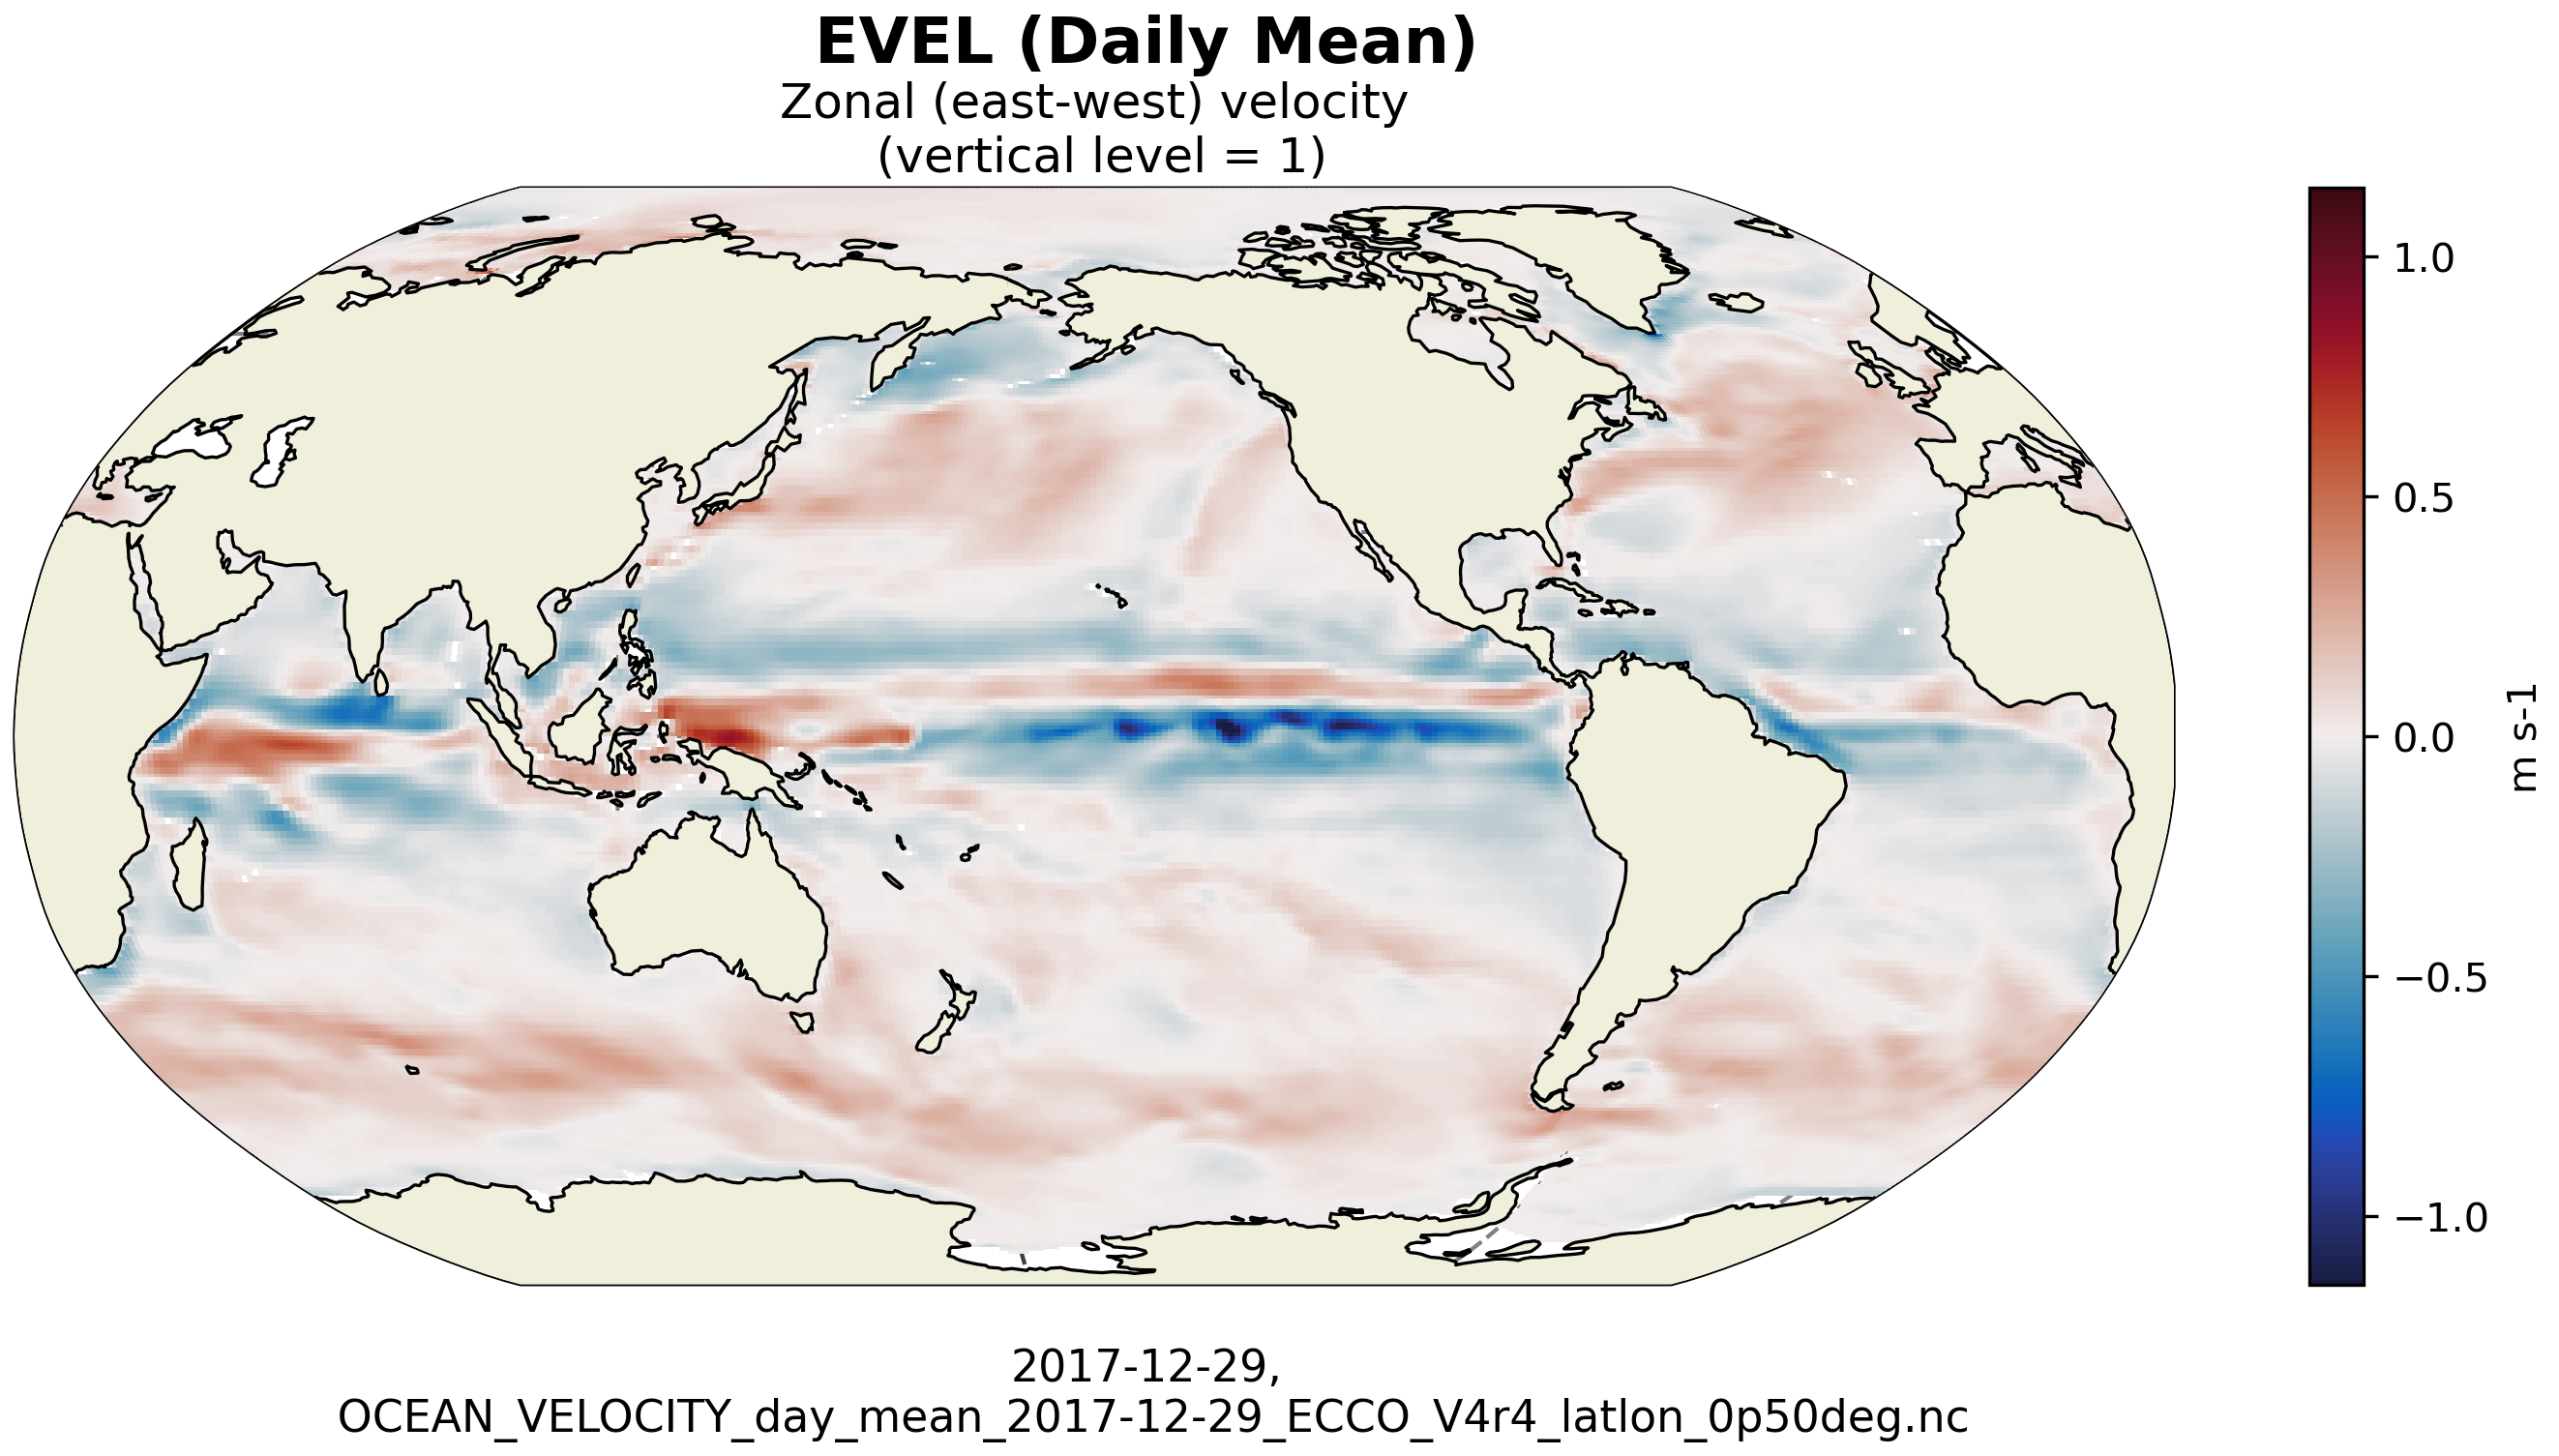
\includegraphics[scale=0.55]{../images/plots/v4r4/latlon_plots/Ocean_Velocity/EVEL.png}
\caption{Dataset: OCEAN\_VELOCITY, Variable: EVEL}
\label{tab:table-OCEAN_VELOCITY_EVEL-Plot}
\end{figure}
\newpage
\pagebreak
\subsubsection{Latlon Variable: NVEL}
\begin{longtable}{|m{0.06\textwidth}|m{0.3\textwidth}|m{0.45\textwidth}|m{0.12\textwidth}|}
\caption{Attributes description of the variable 'NVEL' from OCEAN\_VELOCITY's  dataset.}
\label{tab:table-OCEAN_VELOCITY_NVEL} \\ 
\hline \endhead \hline \endfoot
\rowcolor{lightgray} \textbf{Storage Type} & \textbf{Variable Name} & \textbf{Description} & \textbf{Unit} \\ \hline
float32 & NVEL & Meridional (north-south) velocity & m s-1 \\ \hline
\multicolumn{4}{|c|}{\cellcolor{lightgray}{\textbf{Description of the variable in Common Data language (CDL)}}} \\ \hline
\multicolumn{4}{|c|}{\fontfamily{lmtt}\selectfont{\makecell{\parbox{.95\textwidth}{\vspace*{0.25cm} \footnotesize{float32 NVEL(time, Z, latitude, longitude)\\
\hspace*{0.5cm}NVEL: \_FillValue = 9.96921e+36\\
\hspace*{0.5cm}NVEL: coordinates = Z time\\
\hspace*{0.5cm}NVEL: coverage\_content\_type = modelResult\\
\hspace*{0.5cm}NVEL: long\_name = Meridional (north-south) velocity\\
\hspace*{0.5cm}NVEL: standard\_name = northward sea water velocity\\
\hspace*{0.5cm}NVEL: units = m s-1\\
\hspace*{0.5cm}NVEL: valid\_max = 2.0500051975250244\\
\hspace*{0.5cm}NVEL: valid\_min = -1.2522369623184204\\
}}}}} \\ \hline
\rowcolor{lightgray} \multicolumn{4}{|c|}{\textbf{Comments}} \\ \hline
\multicolumn{4}{|p{1\textwidth}|}{\footnotesize{{Meridional (north-south) component of ocean velocity. note: nvel is calculated by interpolating the model's x and y components of ocean velocity (uvel and vvel) to tracer cell centers and then finding the meridional component of the interpolated vectors. it is not recommended to use evel and nvel for volume budget calculations because interpolating uvel and vvel from the model grid to the lat-lon grid introduces errors. perform volume budget calculations with uvelmass and vvelmass on the native model grid.}}} \\ \hline
\end{longtable}

\begin{figure}[H]
\centering
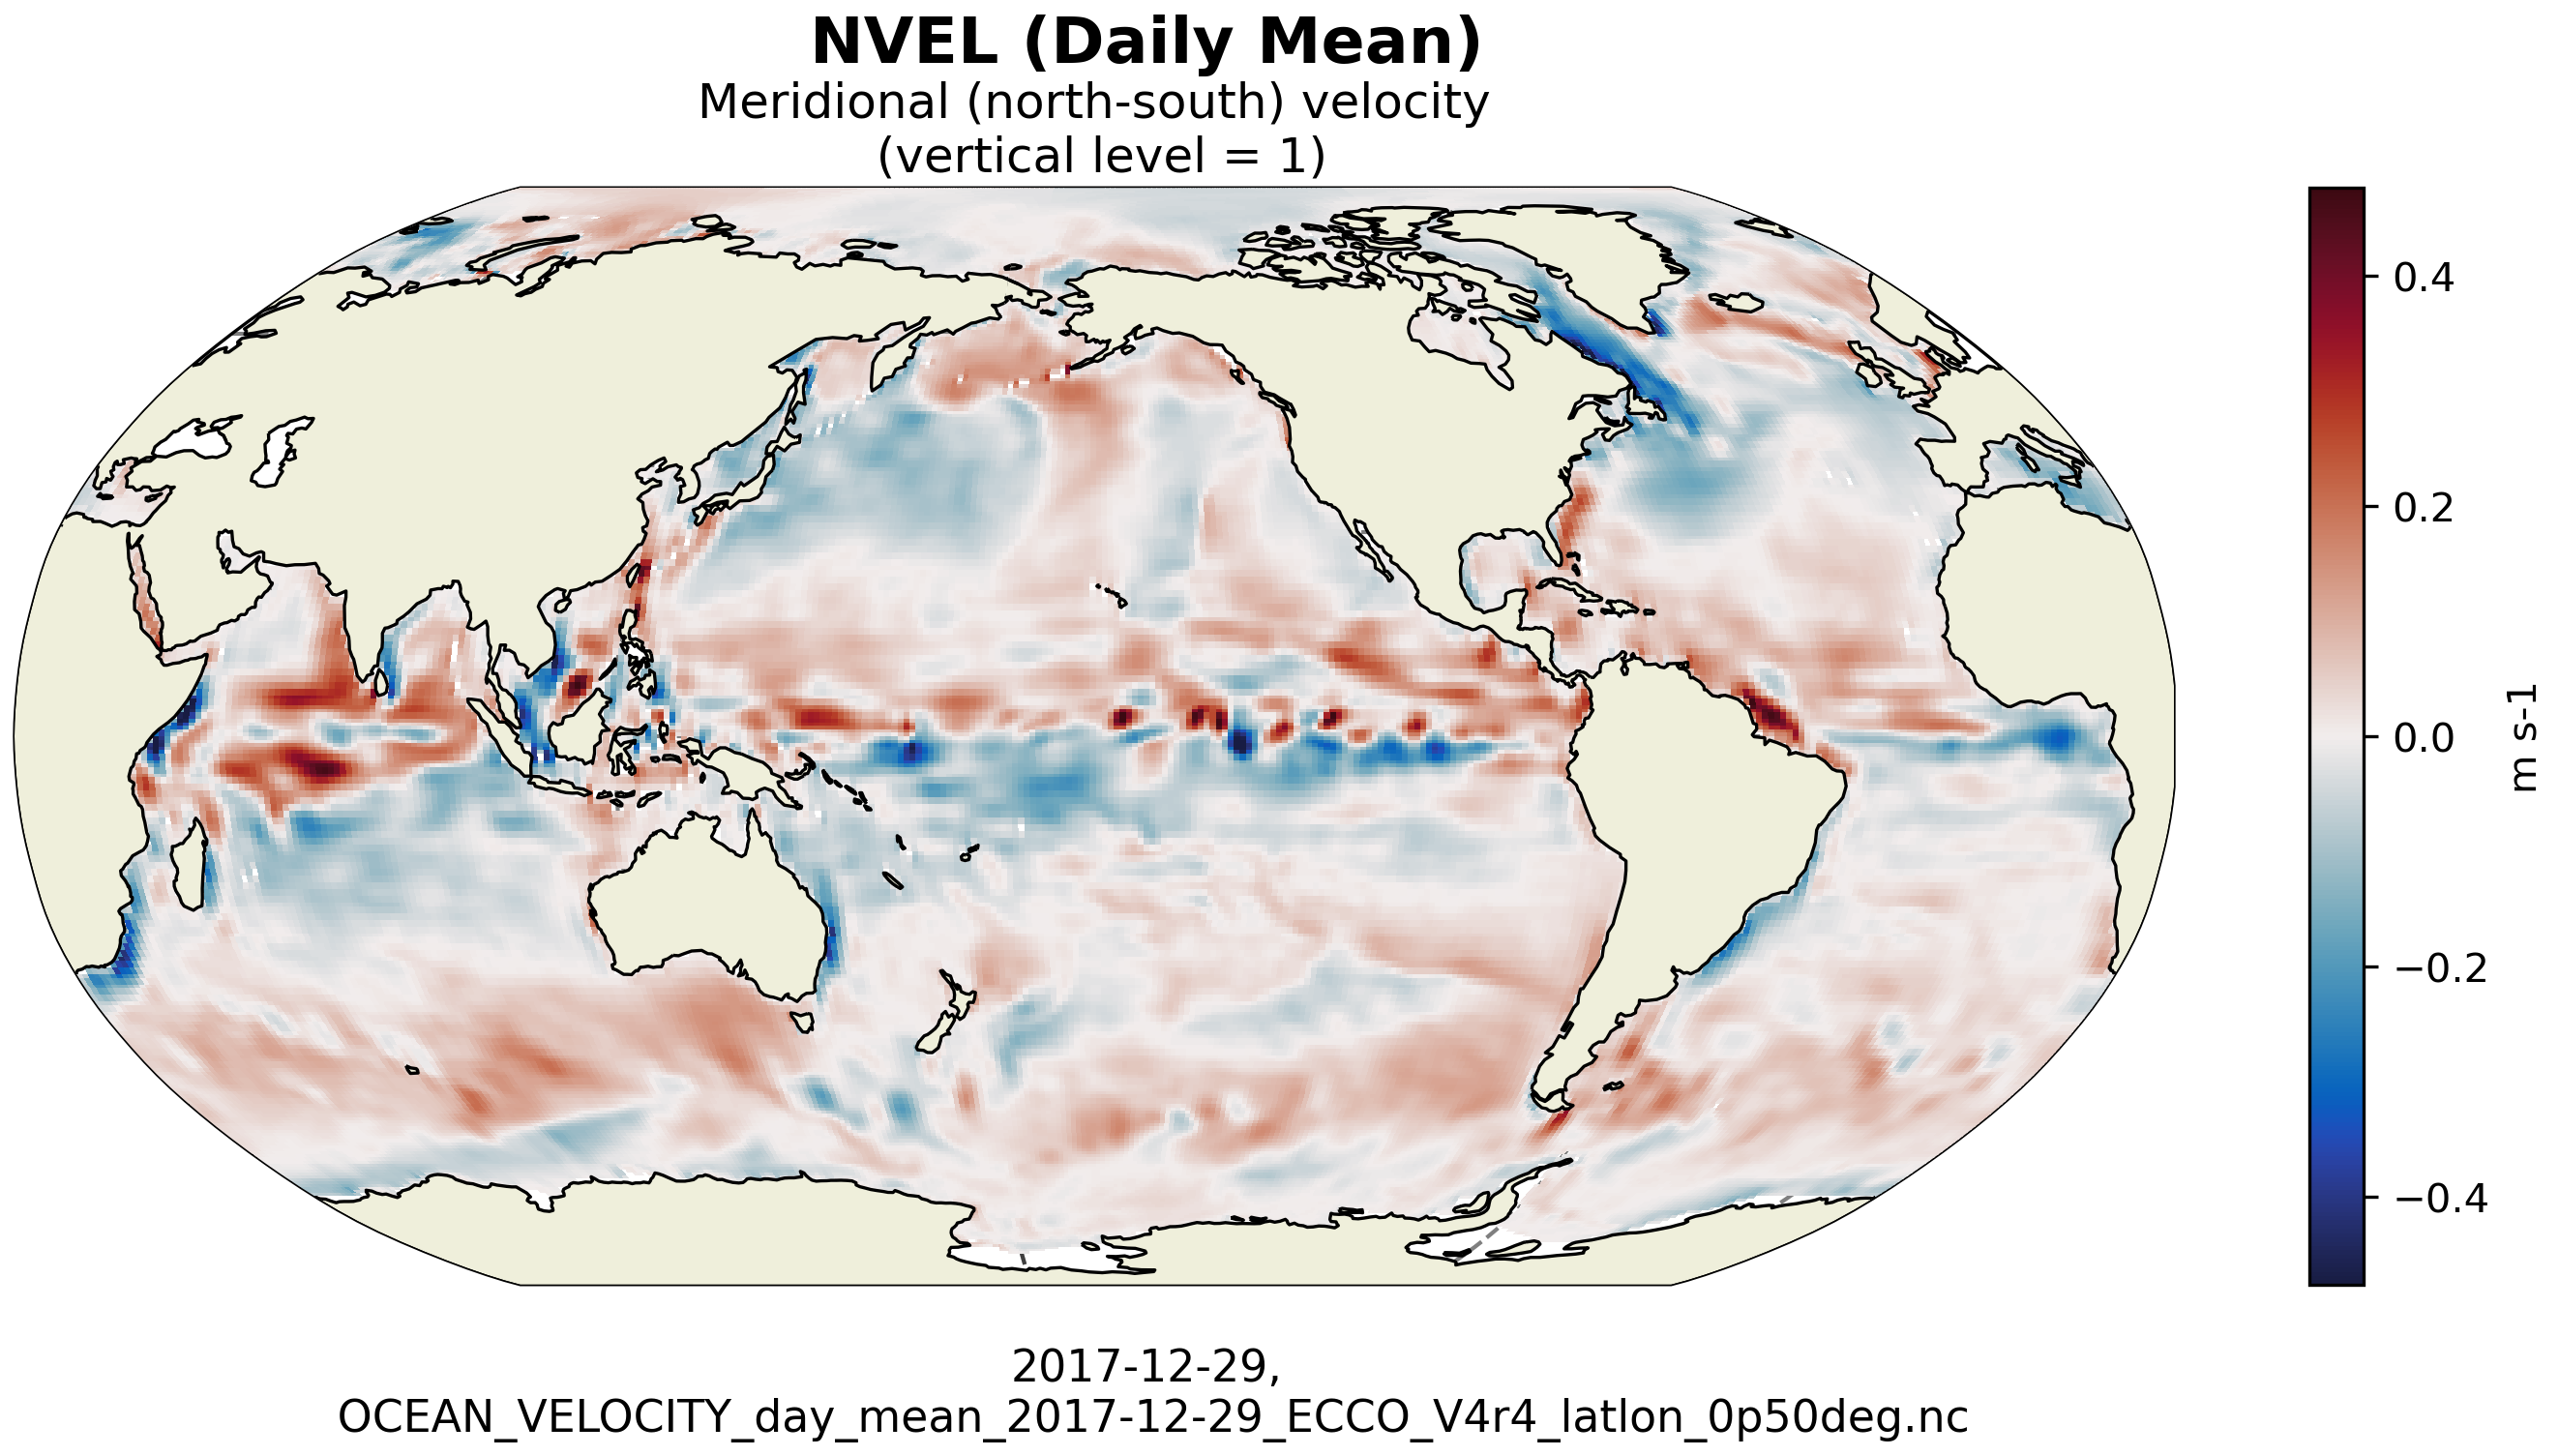
\includegraphics[scale=0.55]{../images/plots/v4r4/latlon_plots/Ocean_Velocity/NVEL.png}
\caption{Dataset: OCEAN\_VELOCITY, Variable: NVEL}
\label{tab:table-OCEAN_VELOCITY_NVEL-Plot}
\end{figure}
\newpage
\pagebreak
\subsubsection{Latlon Variable: WVEL}
\begin{longtable}{|m{0.06\textwidth}|m{0.3\textwidth}|m{0.45\textwidth}|m{0.12\textwidth}|}
\caption{Attributes description of the variable 'WVEL' from OCEAN\_VELOCITY's  dataset.}
\label{tab:table-OCEAN_VELOCITY_WVEL} \\ 
\hline \endhead \hline \endfoot
\rowcolor{lightgray} \textbf{Storage Type} & \textbf{Variable Name} & \textbf{Description} & \textbf{Unit} \\ \hline
float32 & WVEL & Vertical velocity & m s-1 \\ \hline
\multicolumn{4}{|c|}{\cellcolor{lightgray}{\textbf{Description of the variable in Common Data language (CDL)}}} \\ \hline
\multicolumn{4}{|c|}{\fontfamily{lmtt}\selectfont{\makecell{\parbox{.95\textwidth}{\vspace*{0.25cm} \footnotesize{float32 WVEL(time, Z, latitude, longitude)\\
\hspace*{0.5cm}WVEL: \_FillValue = 9.96921e+36\\
\hspace*{0.5cm}WVEL: coordinates = Z time\\
\hspace*{0.5cm}WVEL: coverage\_content\_type = modelResult\\
\hspace*{0.5cm}WVEL: direction = >0 decreases volume\\
\hspace*{0.5cm}WVEL: long\_name = Vertical velocity\\
\hspace*{0.5cm}WVEL: standard\_name = upward sea water velocity\\
\hspace*{0.5cm}WVEL: units = m s-1\\
\hspace*{0.5cm}WVEL: valid\_max = 0.0016380994347855449\\
\hspace*{0.5cm}WVEL: valid\_min = -0.0023150660563260317\\
}}}}} \\ \hline
\rowcolor{lightgray} \multicolumn{4}{|c|}{\textbf{Comments}} \\ \hline
\multicolumn{4}{|p{1\textwidth}|}{\footnotesize{{Vertical velocity in the +z direction at the top face of the grid cell. note: in the arakawa-c grid used in ecco v4r4, vertical velocities are staggered relative to the tracer cell centers with values at the top and bottom faces of each grid cell.}}} \\ \hline
\end{longtable}

\begin{figure}[H]
\centering
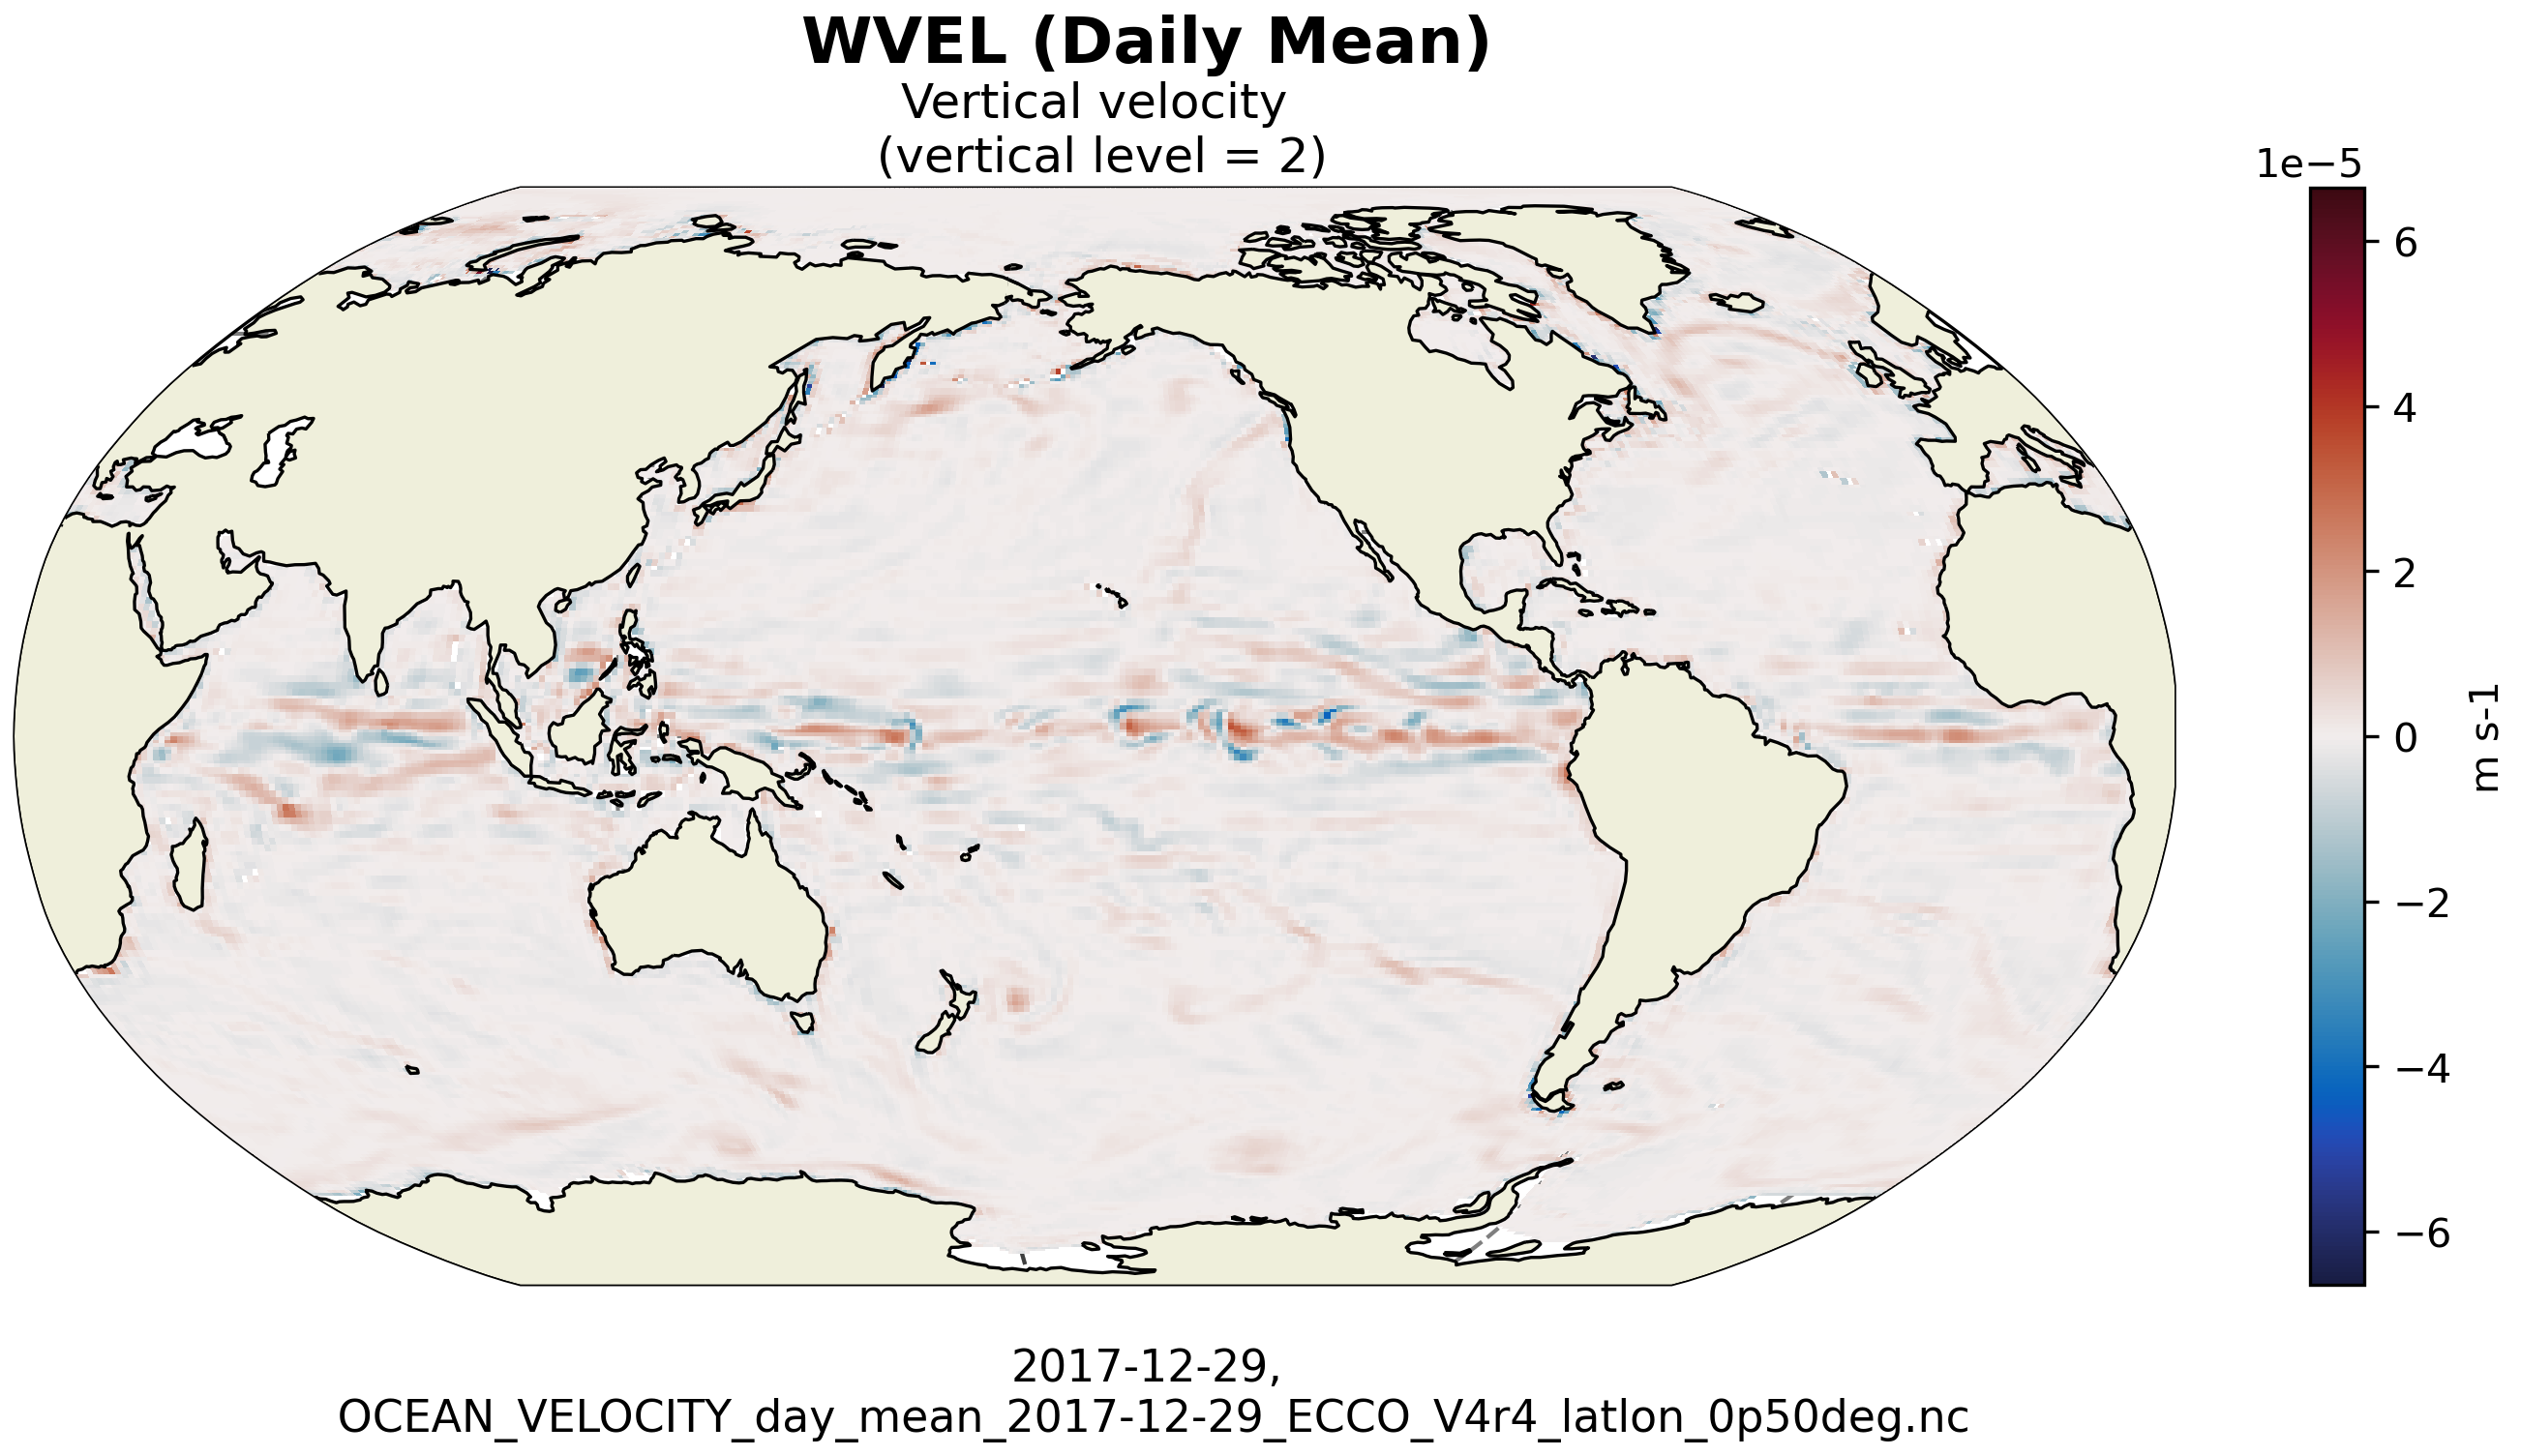
\includegraphics[scale=0.55]{../images/plots/v4r4/latlon_plots/Ocean_Velocity/WVEL.png}
\caption{Dataset: OCEAN\_VELOCITY, Variable: WVEL}
\label{tab:table-OCEAN_VELOCITY_WVEL-Plot}
\end{figure}
\newpage
\subsection{Latlon dataset of SEA\_ICE\_CONC\_THICKNESS}
\newp
\subsubsection{Overview}
This dataset provides 2D fields of sea-ice and snow concentration and thickness interpolated to a regular 0.5-degree grid from the ECCO Version 4 Release 4 (V4r4) ocean and sea-ice state estimate. The dataset is provided on daily-average and monthly-average time resolution. 
\begin{longtable}{|m{0.15\textwidth}|m{0.64\textwidth}|m{0.12\textwidth}|}
\caption{Coordinates and Variables in the dataset SEA\_ICE\_CONC\_THICKNESS}
\label{tab:table-SEA_ICE_CONC_THICKNESS-fields} \\ 
\hline \endhead \hline \endfoot
\rowcolor{lightgray} \multicolumn{1}{|c|}{\textbf{Coordinates}} & \multicolumn{1}{|c|}{\textbf{Description of data coordinates}} &  \multicolumn{1}{|c|}{\textbf{Unit}}\\ \hline
time &Center time of averaging period &--none--  \\ \hline
latitude &Latitude at grid cell center &degrees\_north  \\ \hline
longitude &Longitude at grid cell center &degrees\_east  \\ \hline
time\_bnds &Time bounds of averaging period &--none--  \\ \hline
latitude\_bnds &Latitude bounds grid cells &--none--  \\ \hline
longitude\_bnds &Longitude bounds grid cells &--none--  \\ \hline
\rowcolor{lightgray} \multicolumn{1}{|c|}{\textbf{Variables}} & \multicolumn{1}{|c|}{\textbf{Description of data variables}} &  \multicolumn{1}{|c|}{\textbf{Unit}}\\ \hline
SIarea &Sea-ice concentration &1  \\ \hline
SIheff &Area-averaged sea-ice thickness &m  \\ \hline
SIhsnow &Area-averaged snow thickness &m  \\ \hline
sIceLoad &Average sea-ice and snow mass per unit area &kg m-2  \\ \hline
\end{longtable}

\newp
\pagebreak
\subsubsection{Latlon Variable: SIarea}
\begin{longtable}{|m{0.06\textwidth}|m{0.3\textwidth}|m{0.45\textwidth}|m{0.12\textwidth}|}
\caption{Attributes description of the variable 'SIarea' from SEA\_ICE\_CONC\_THICKNESS's  dataset.}
\label{tab:table-SEA_ICE_CONC_THICKNESS_SIarea} \\ 
\hline \endhead \hline \endfoot
\rowcolor{lightgray} \textbf{Storage Type} & \textbf{Variable Name} & \textbf{Description} & \textbf{Unit} \\ \hline
float32 & SIarea & Sea-ice concentration & 1 \\ \hline
\multicolumn{4}{|c|}{\cellcolor{lightgray}{\textbf{Description of the variable in Common Data language (CDL)}}} \\ \hline
\multicolumn{4}{|c|}{\fontfamily{lmtt}\selectfont{\makecell{\parbox{.95\textwidth}{\vspace*{0.25cm} \footnotesize{float32 SIarea(time, latitude, longitude)\\
\hspace*{0.5cm}SIarea: \_FillValue = 9.96921e+36\\
\hspace*{0.5cm}SIarea: coordinates = time\\
\hspace*{0.5cm}SIarea: coverage\_content\_type = modelResult\\
\hspace*{0.5cm}SIarea: long\_name = Sea-ice concentration\\
\hspace*{0.5cm}SIarea: standard\_name = sea ice area fraction\\
\hspace*{0.5cm}SIarea: units = 1\\
\hspace*{0.5cm}SIarea: valid\_max = 0.9700000286102295\\
\hspace*{0.5cm}SIarea: valid\_min = 0.0\\
}}}}} \\ \hline
\rowcolor{lightgray} \multicolumn{4}{|c|}{\textbf{Comments}} \\ \hline
\multicolumn{4}{|p{1\textwidth}|}{\footnotesize{{Fraction of ocean grid cell covered with sea-ice [0 to 1]. cf standard name table v73:  'area fraction' is the fraction of a grid cell's horizontal area that has some characteristic of interest. it is evaluated as the area of interest divided by the grid cell area. it may be expressed as a fraction, a percentage, or any other dimensionless representation of a fraction. sea ice area fraction is area of the sea surface occupied by sea ice. it is also called 'sea ice concentration'. 'sea ice' means all ice floating in the sea which has formed from freezing sea water, rather than by other processes such as calving of land ice to form icebergs. https://cfconventions.org/data/cf-standard-names/73/build/cf-standard-name-table.html. defined using cf standard name table v73: 'area fraction' is the fraction of a grid cell's horizontal area that has some characteristic of interest. it is evaluated as the area of interest divided by the grid cell area. it may be expressed as a fraction, a percentage, or any other dimensionless representation of a fraction. sea ice area fraction is area of the sea surface occupied by sea ice. it is also called 'sea ice concentration'. 'sea ice' means all ice floating in the sea which has formed from freezing sea water and precipitation, rather than by other processes such as calving of land ice to form icebergs. https://cfconventions.org/data/cf-standard-names/73/build/cf-standard-name-table.html}}} \\ \hline
\end{longtable}

\begin{figure}[H]
\centering
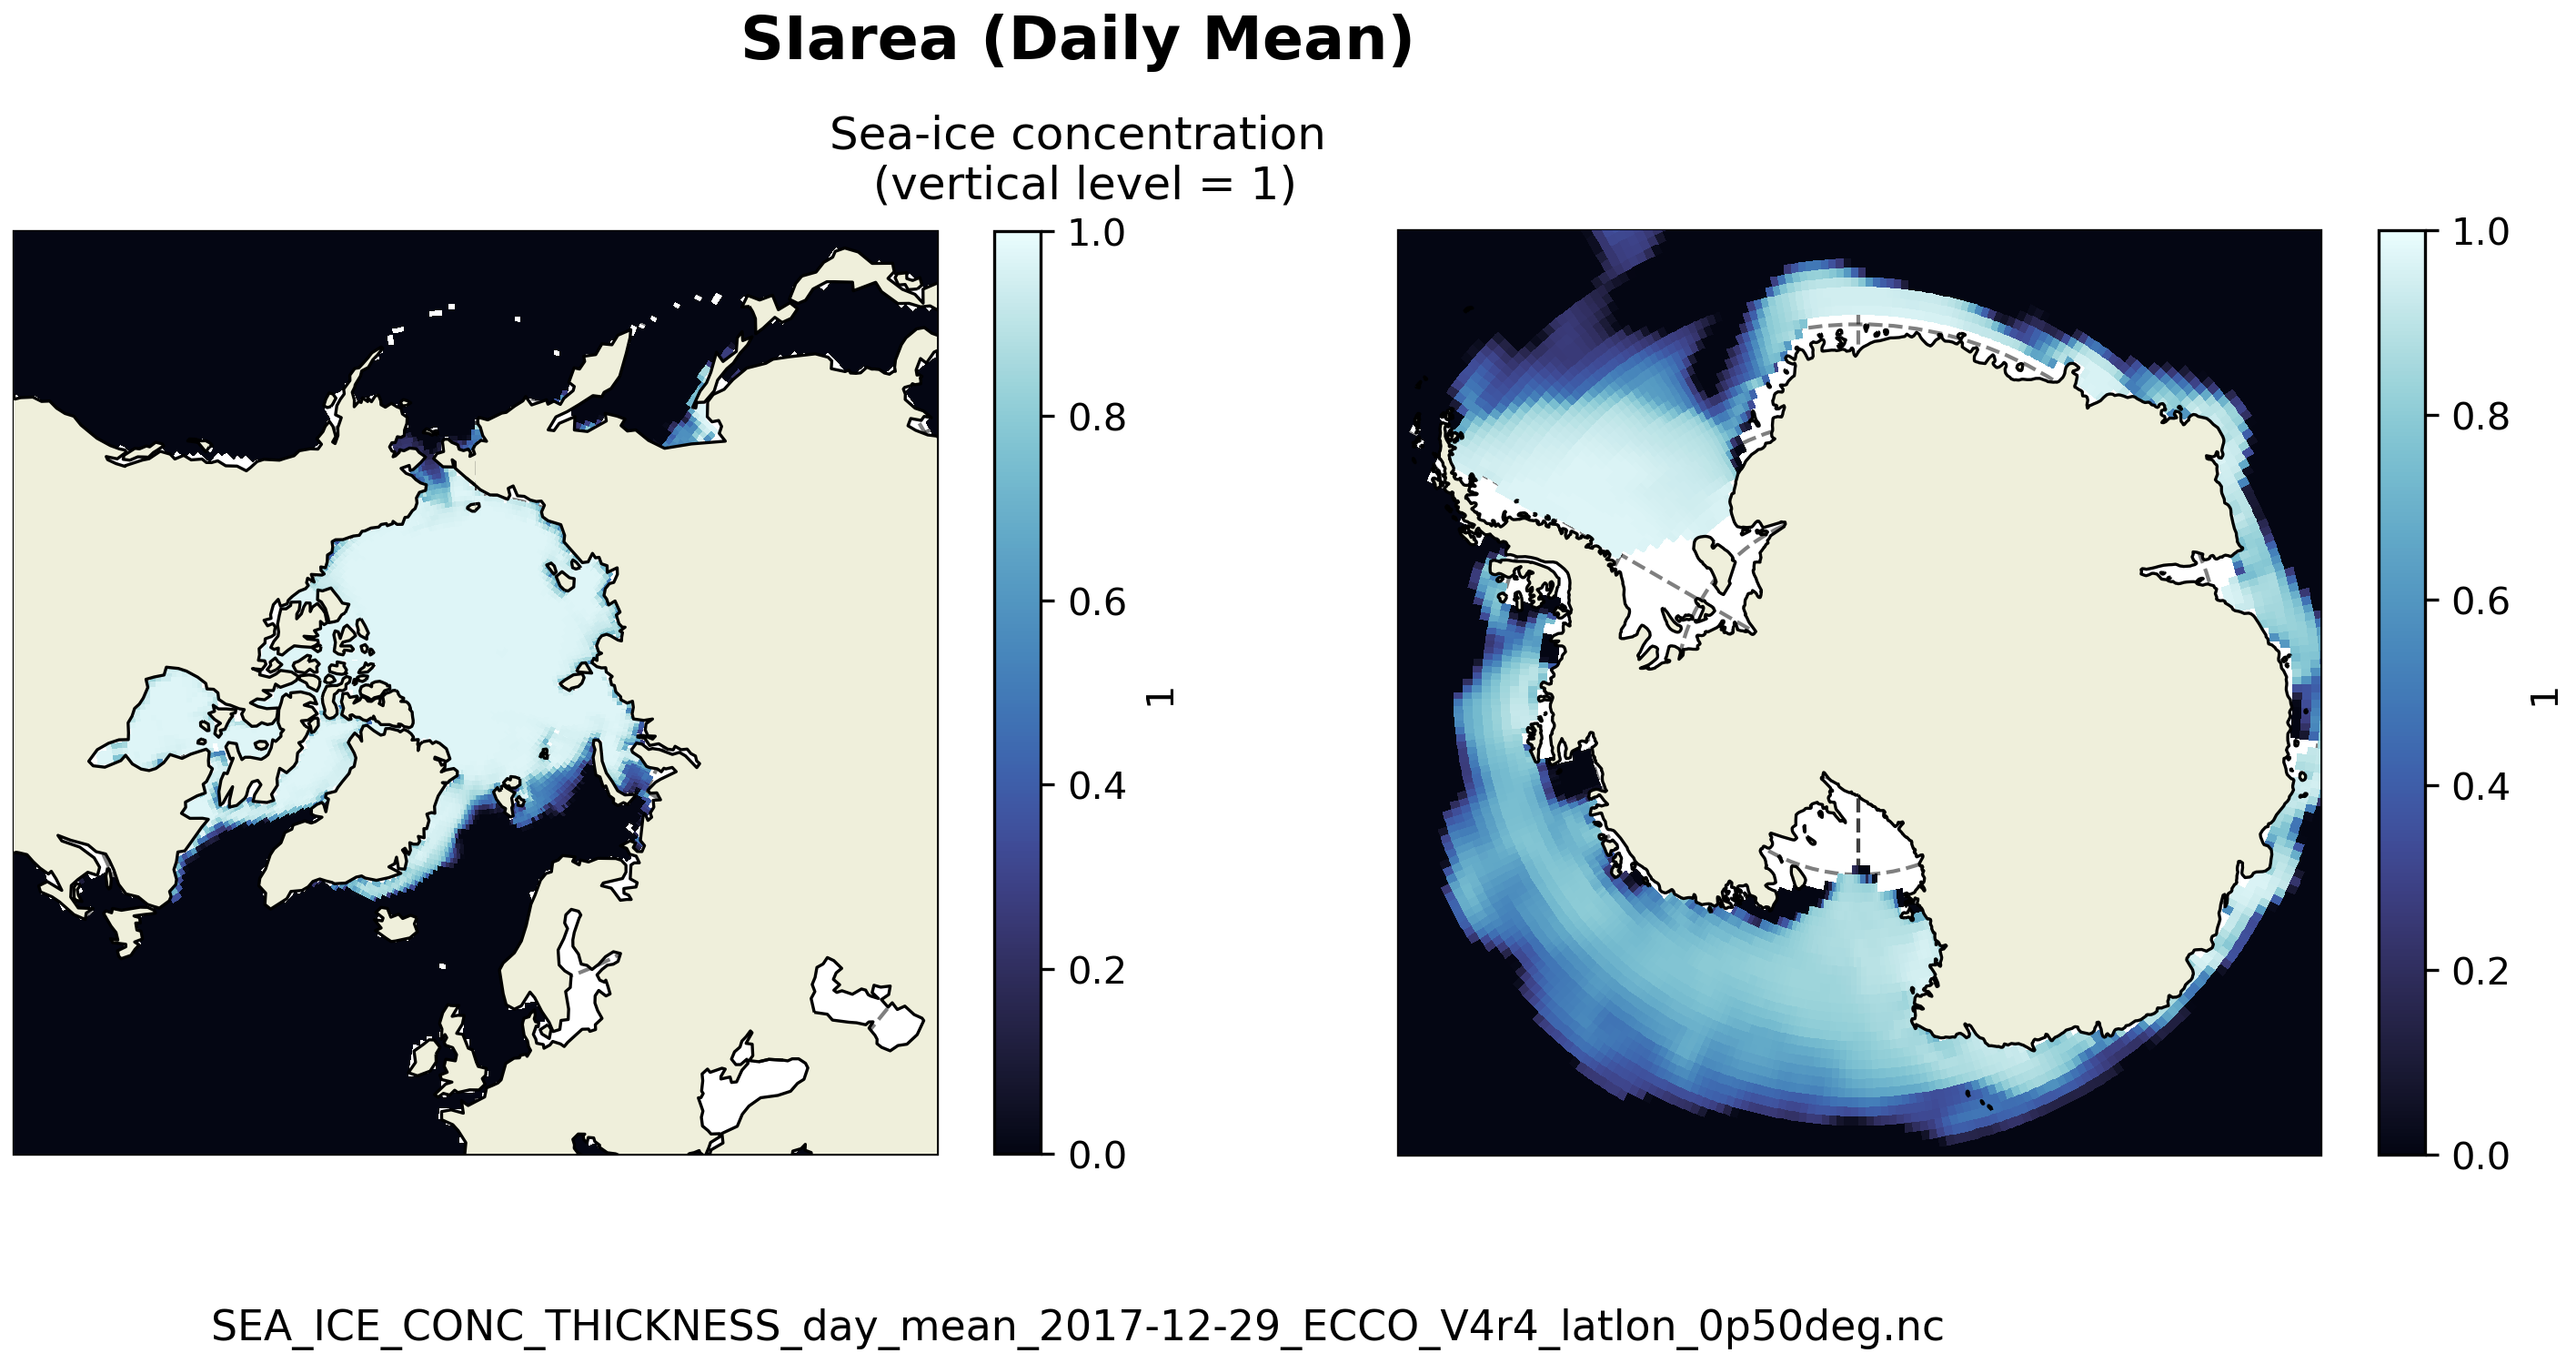
\includegraphics[scale=0.55]{../images/plots/v4r4/latlon_plots/Sea-Ice_and_Snow_Concentration_and_Thickness/SIarea.png}
\caption{Dataset: SEA\_ICE\_CONC\_THICKNESS, Variable: SIarea}
\label{tab:table-SEA_ICE_CONC_THICKNESS_SIarea-Plot}
\end{figure}
\newpage
\pagebreak
\subsubsection{Latlon Variable: SIheff}
\begin{longtable}{|m{0.06\textwidth}|m{0.3\textwidth}|m{0.45\textwidth}|m{0.12\textwidth}|}
\caption{Attributes description of the variable 'SIheff' from SEA\_ICE\_CONC\_THICKNESS's  dataset.}
\label{tab:table-SEA_ICE_CONC_THICKNESS_SIheff} \\ 
\hline \endhead \hline \endfoot
\rowcolor{lightgray} \textbf{Storage Type} & \textbf{Variable Name} & \textbf{Description} & \textbf{Unit} \\ \hline
float32 & SIheff & Area-averaged sea-ice thickness & m \\ \hline
\multicolumn{4}{|c|}{\cellcolor{lightgray}{\textbf{Description of the variable in Common Data language (CDL)}}} \\ \hline
\multicolumn{4}{|c|}{\fontfamily{lmtt}\selectfont{\makecell{\parbox{.95\textwidth}{\vspace*{0.25cm} \footnotesize{float32 SIheff(time, latitude, longitude)\\
\hspace*{0.5cm}SIheff: \_FillValue = 9.96921e+36\\
\hspace*{0.5cm}SIheff: coordinates = time\\
\hspace*{0.5cm}SIheff: coverage\_content\_type = modelResult\\
\hspace*{0.5cm}SIheff: long\_name = Area-averaged sea-ice thickness\\
\hspace*{0.5cm}SIheff: standard\_name = sea ice thickness\\
\hspace*{0.5cm}SIheff: units = m\\
\hspace*{0.5cm}SIheff: valid\_max = 9.000518798828125\\
\hspace*{0.5cm}SIheff: valid\_min = 0.0\\
}}}}} \\ \hline
\rowcolor{lightgray} \multicolumn{4}{|c|}{\textbf{Comments}} \\ \hline
\multicolumn{4}{|p{1\textwidth}|}{\footnotesize{{Sea-ice thickness averaged over the entire model grid cell, including open water where sea-ice thickness is zero. note: sea-ice thickness over the ice-covered fraction of the grid cell is siheff/siarea}}} \\ \hline
\end{longtable}

\begin{figure}[H]
\centering
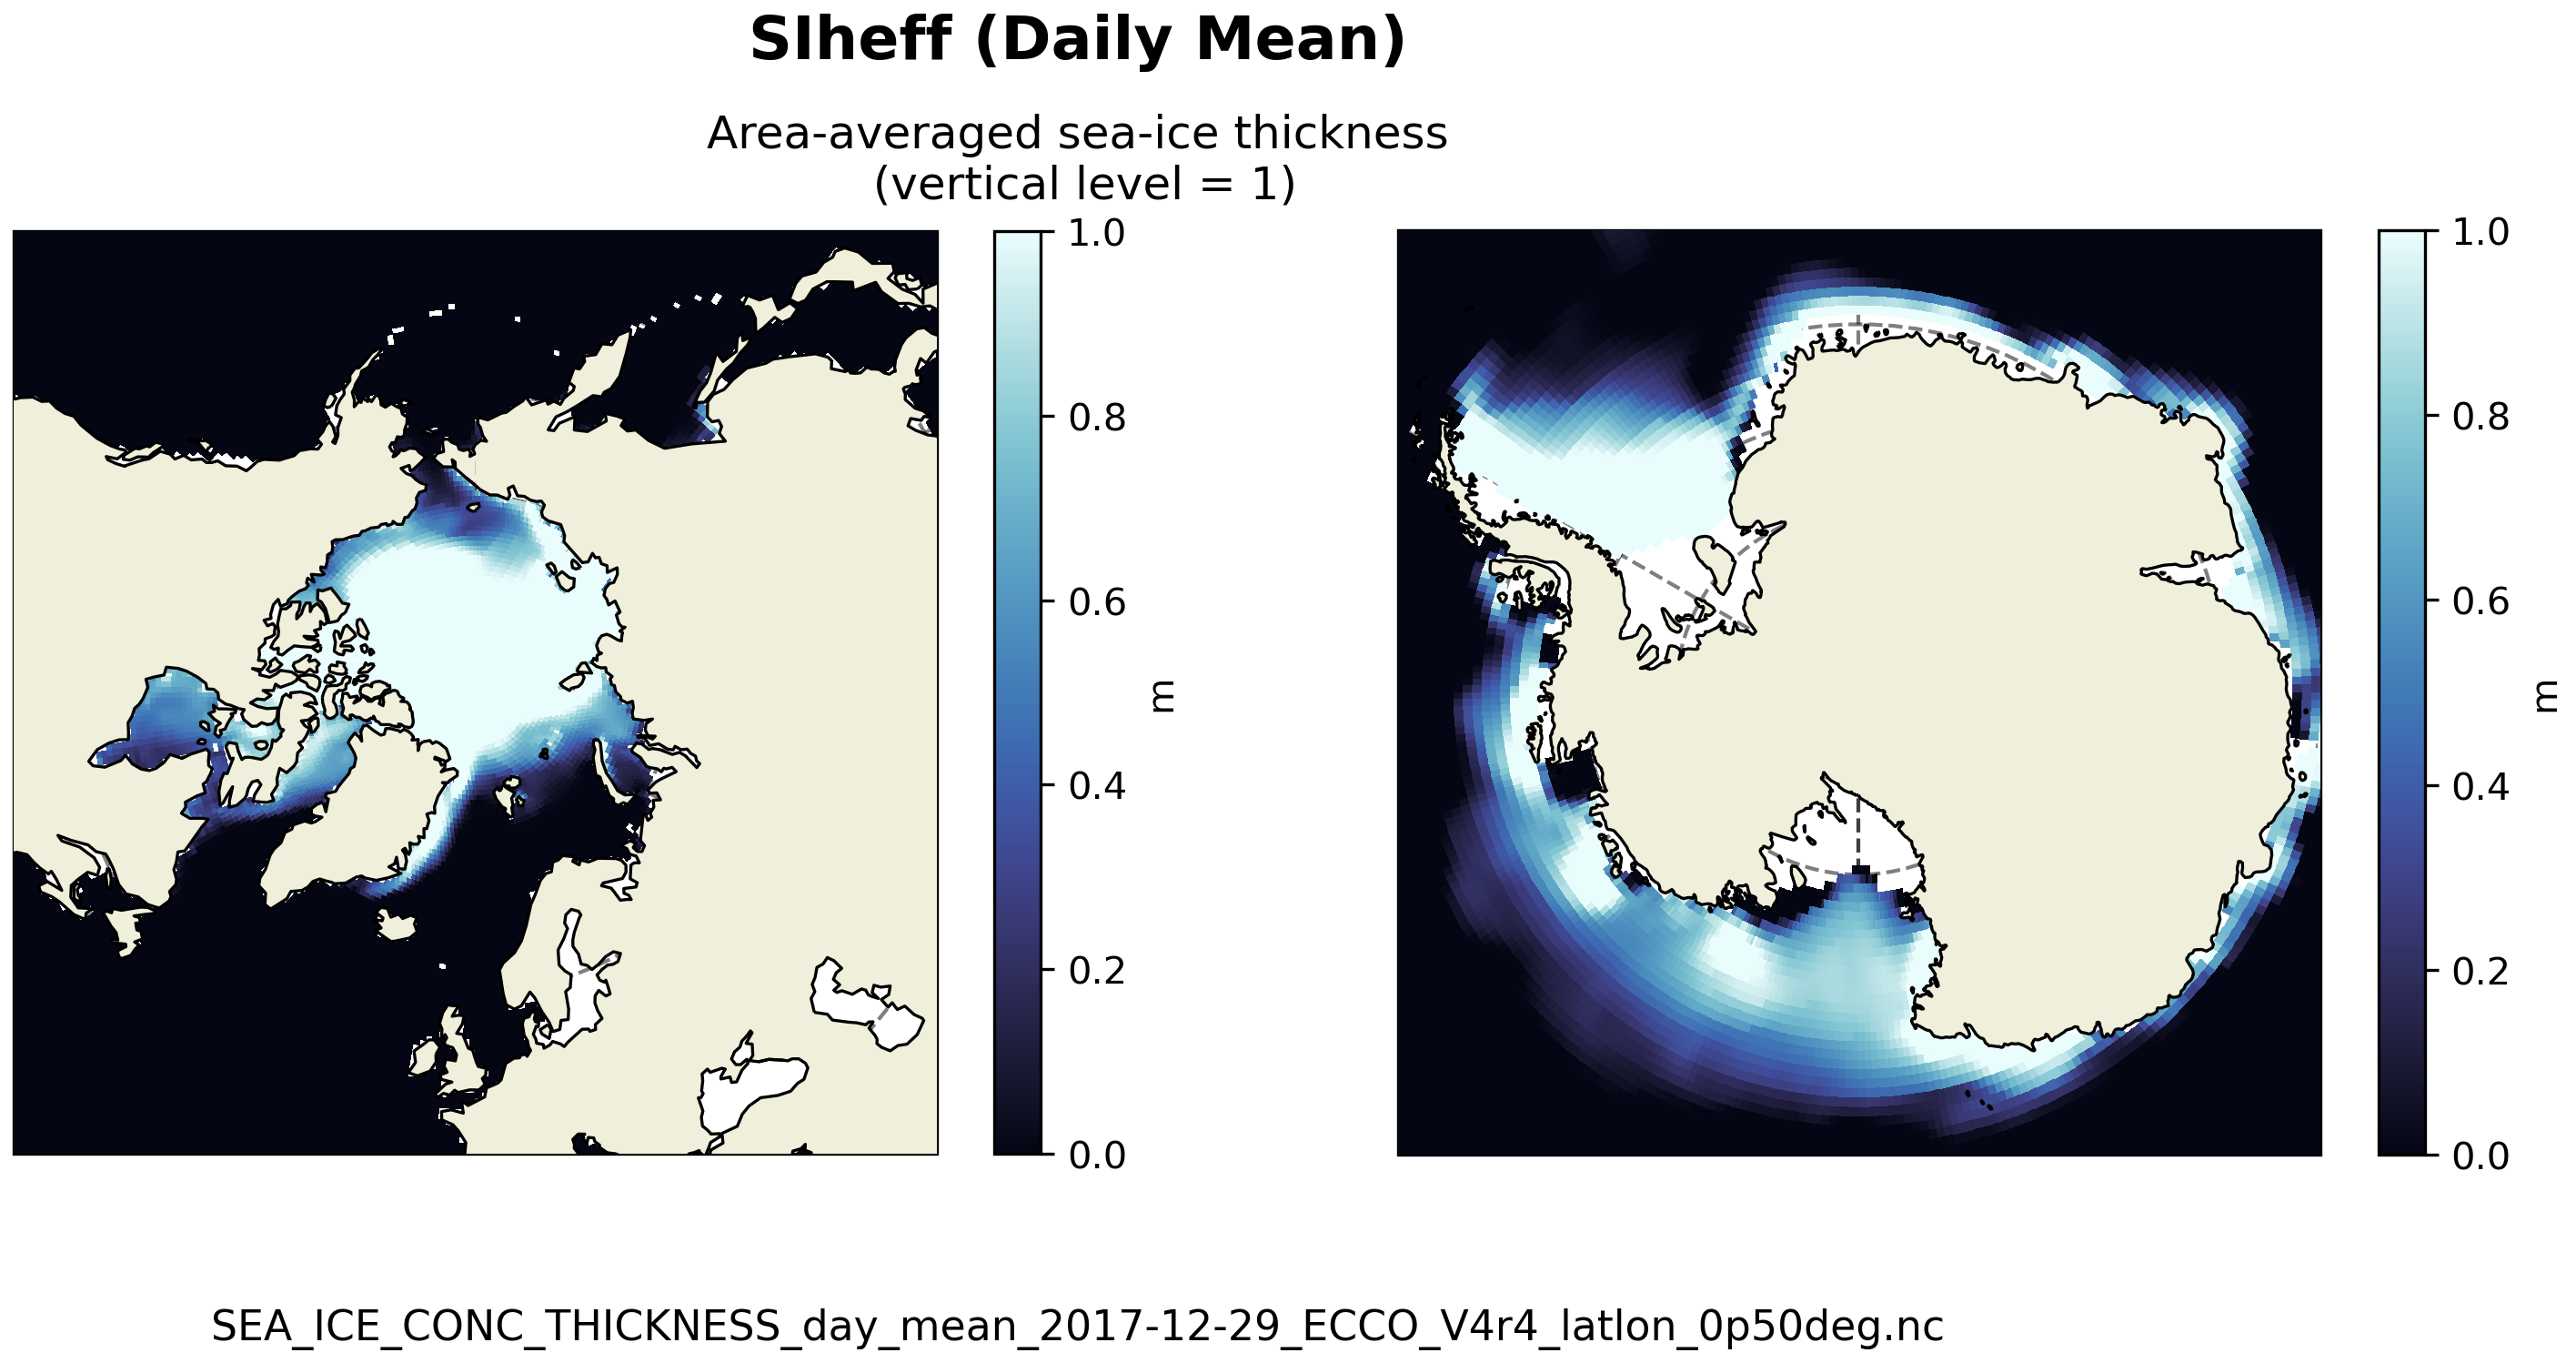
\includegraphics[scale=0.55]{../images/plots/v4r4/latlon_plots/Sea-Ice_and_Snow_Concentration_and_Thickness/SIheff.png}
\caption{Dataset: SEA\_ICE\_CONC\_THICKNESS, Variable: SIheff}
\label{tab:table-SEA_ICE_CONC_THICKNESS_SIheff-Plot}
\end{figure}
\newpage
\pagebreak
\subsubsection{Latlon Variable: SIhsnow}
\begin{longtable}{|m{0.06\textwidth}|m{0.3\textwidth}|m{0.45\textwidth}|m{0.12\textwidth}|}
\caption{Attributes description of the variable 'SIhsnow' from SEA\_ICE\_CONC\_THICKNESS's  dataset.}
\label{tab:table-SEA_ICE_CONC_THICKNESS_SIhsnow} \\ 
\hline \endhead \hline \endfoot
\rowcolor{lightgray} \textbf{Storage Type} & \textbf{Variable Name} & \textbf{Description} & \textbf{Unit} \\ \hline
float32 & SIhsnow & Area-averaged snow thickness & m \\ \hline
\multicolumn{4}{|c|}{\cellcolor{lightgray}{\textbf{Description of the variable in Common Data language (CDL)}}} \\ \hline
\multicolumn{4}{|c|}{\fontfamily{lmtt}\selectfont{\makecell{\parbox{.95\textwidth}{\vspace*{0.25cm} \footnotesize{float32 SIhsnow(time, latitude, longitude)\\
\hspace*{0.5cm}SIhsnow: \_FillValue = 9.96921e+36\\
\hspace*{0.5cm}SIhsnow: coordinates = time\\
\hspace*{0.5cm}SIhsnow: coverage\_content\_type = modelResult\\
\hspace*{0.5cm}SIhsnow: long\_name = Area-averaged snow thickness\\
\hspace*{0.5cm}SIhsnow: standard\_name = surface snow thickness\\
\hspace*{0.5cm}SIhsnow: units = m\\
\hspace*{0.5cm}SIhsnow: valid\_max = 2.5671639442443848\\
\hspace*{0.5cm}SIhsnow: valid\_min = -0.0004725505714304745\\
}}}}} \\ \hline
\rowcolor{lightgray} \multicolumn{4}{|c|}{\textbf{Comments}} \\ \hline
\multicolumn{4}{|p{1\textwidth}|}{\footnotesize{{Snow thickness averaged over the entire model grid cell, including open water where snow thickness is zero. note: snow thickness over the ice-covered fraction of the grid cell is sihsnow/siarea}}} \\ \hline
\end{longtable}

\begin{figure}[H]
\centering
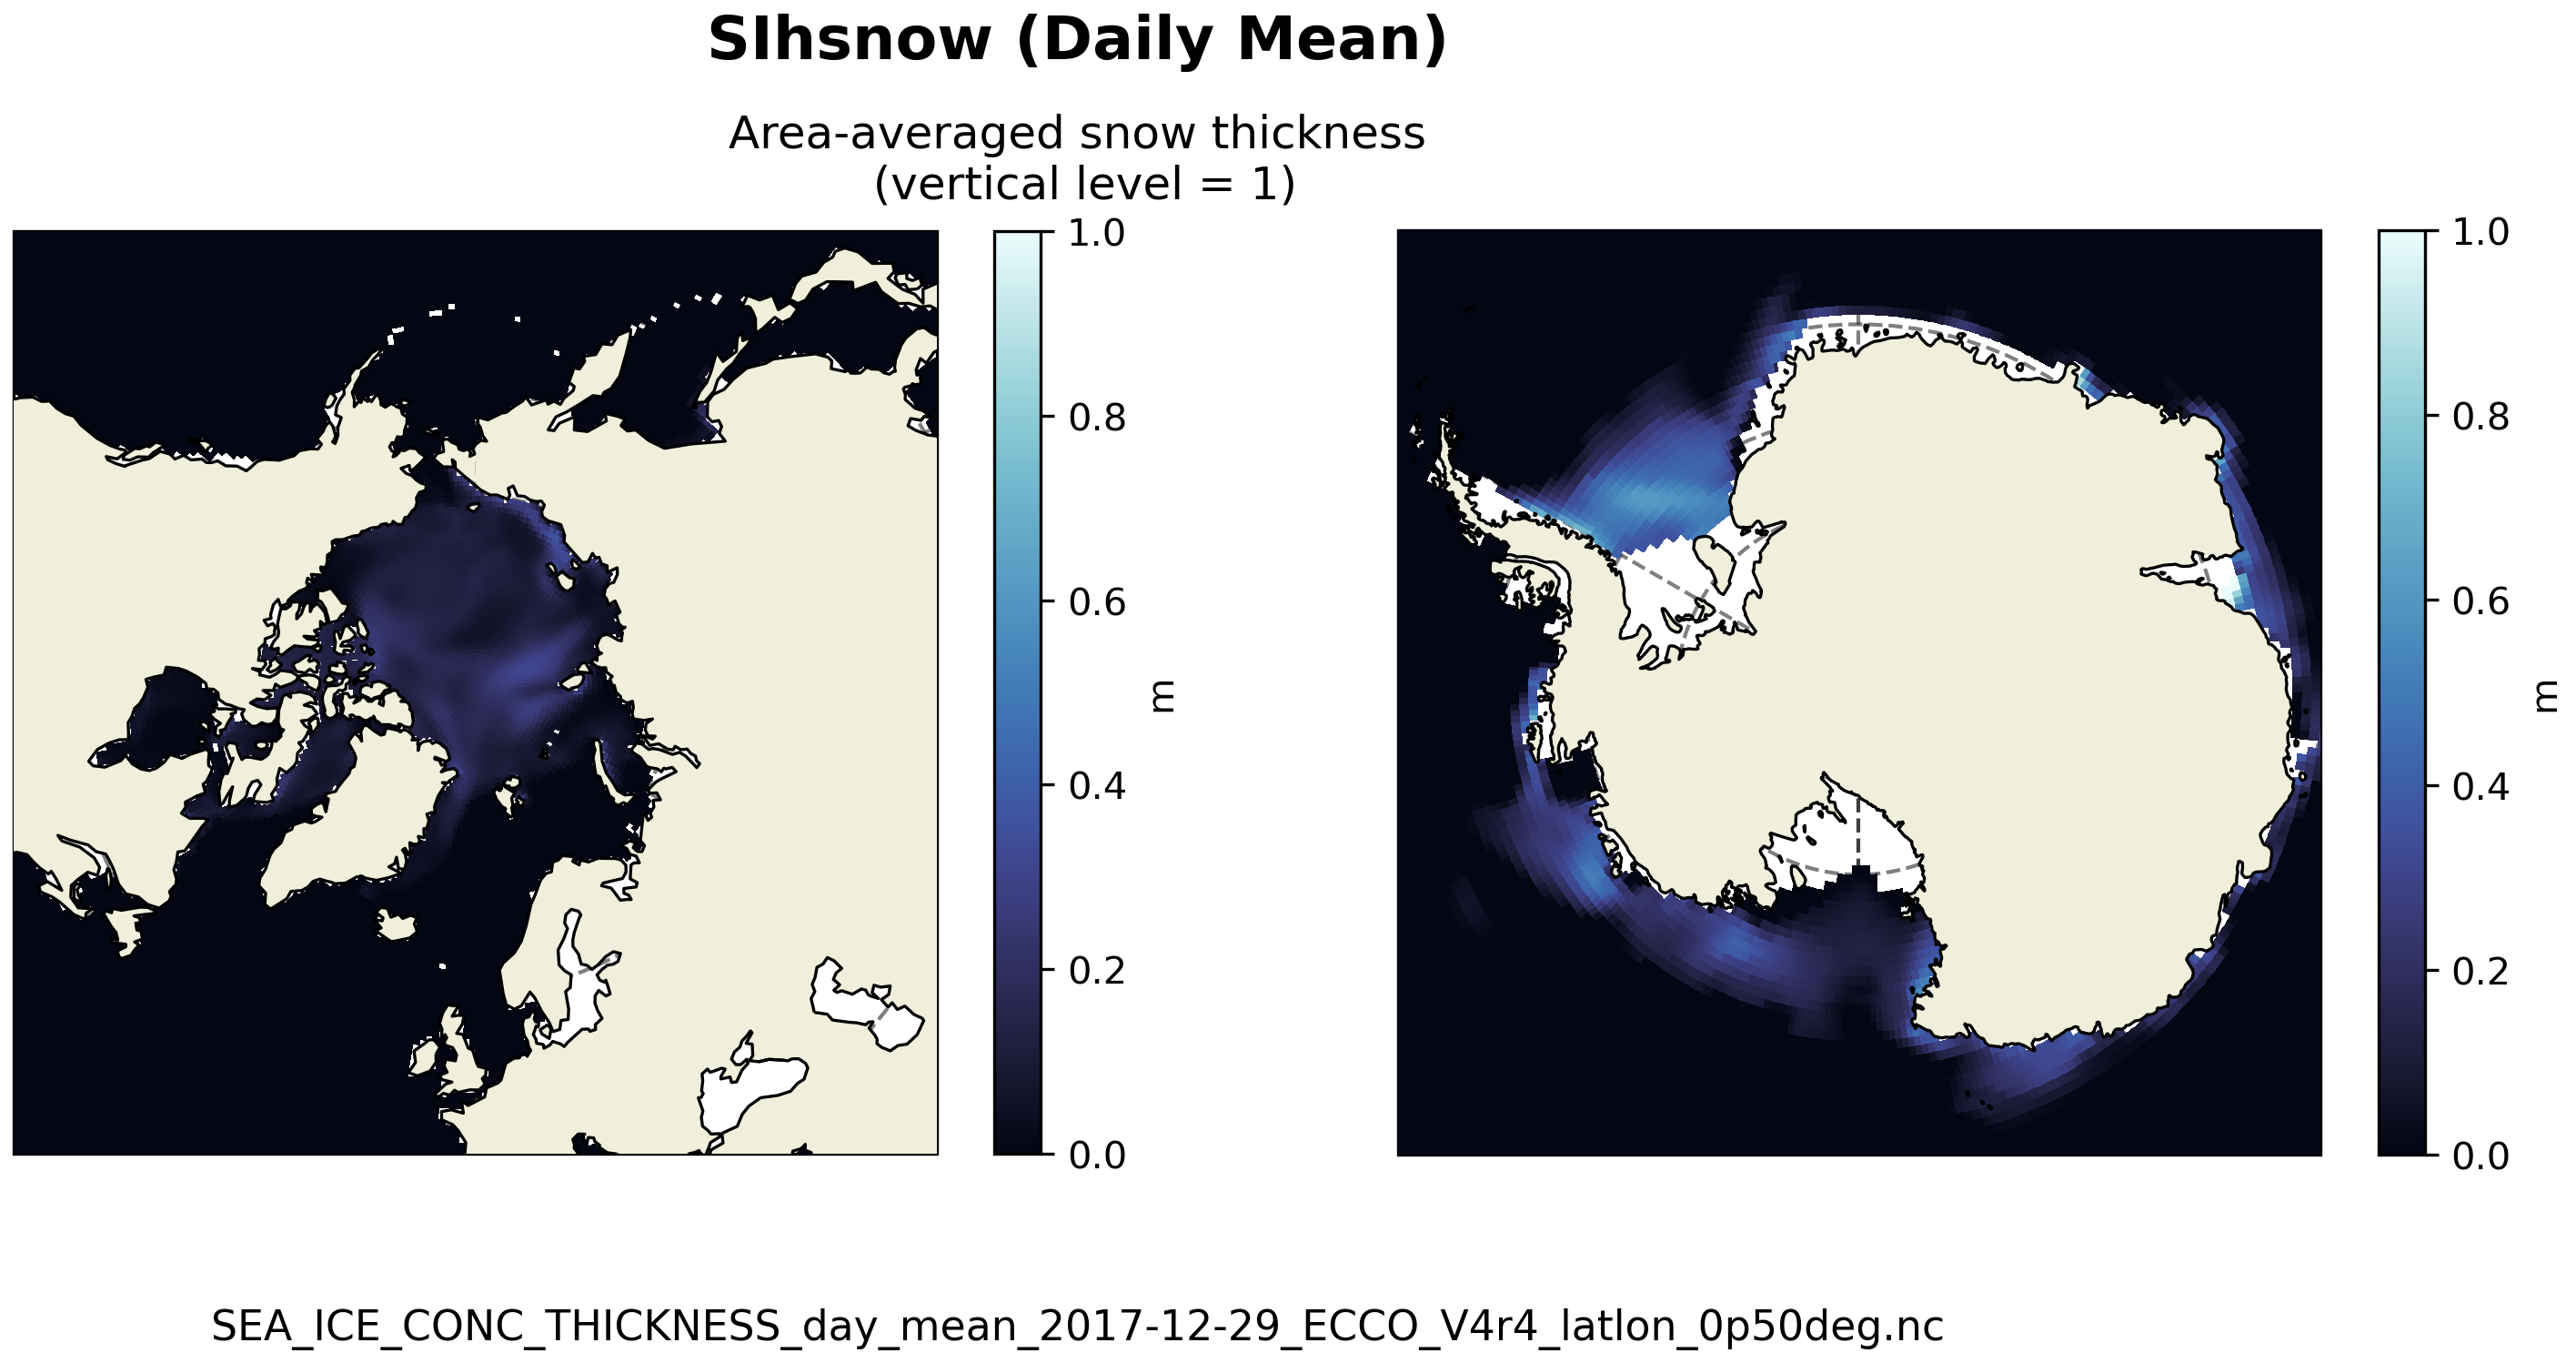
\includegraphics[scale=0.55]{../images/plots/v4r4/latlon_plots/Sea-Ice_and_Snow_Concentration_and_Thickness/SIhsnow.png}
\caption{Dataset: SEA\_ICE\_CONC\_THICKNESS, Variable: SIhsnow}
\label{tab:table-SEA_ICE_CONC_THICKNESS_SIhsnow-Plot}
\end{figure}
\newpage
\pagebreak
\subsubsection{Latlon Variable: sIceLoad}
\begin{longtable}{|m{0.06\textwidth}|m{0.3\textwidth}|m{0.45\textwidth}|m{0.12\textwidth}|}
\caption{Attributes description of the variable 'sIceLoad' from SEA\_ICE\_CONC\_THICKNESS's  dataset.}
\label{tab:table-SEA_ICE_CONC_THICKNESS_sIceLoad} \\ 
\hline \endhead \hline \endfoot
\rowcolor{lightgray} \textbf{Storage Type} & \textbf{Variable Name} & \textbf{Description} & \textbf{Unit} \\ \hline
float32 & sIceLoad & Average sea-ice and snow mass per unit area & kg m-2 \\ \hline
\multicolumn{4}{|c|}{\cellcolor{lightgray}{\textbf{Description of the variable in Common Data language (CDL)}}} \\ \hline
\multicolumn{4}{|c|}{\fontfamily{lmtt}\selectfont{\makecell{\parbox{.95\textwidth}{\vspace*{0.25cm} \footnotesize{float32 sIceLoad(time, latitude, longitude)\\
\hspace*{0.5cm}sIceLoad: \_FillValue = 9.96921e+36\\
\hspace*{0.5cm}sIceLoad: coordinates = time\\
\hspace*{0.5cm}sIceLoad: coverage\_content\_type = modelResult\\
\hspace*{0.5cm}sIceLoad: long\_name = Average sea-ice and snow mass per unit area\\
\hspace*{0.5cm}sIceLoad: standard\_name = sea ice and surface snow amount\\
\hspace*{0.5cm}sIceLoad: units = kg m-2\\
\hspace*{0.5cm}sIceLoad: valid\_max = 8729.935546875\\
\hspace*{0.5cm}sIceLoad: valid\_min = -0.0015558383893221617\\
}}}}} \\ \hline
\rowcolor{lightgray} \multicolumn{4}{|c|}{\textbf{Comments}} \\ \hline
\multicolumn{4}{|p{1\textwidth}|}{\footnotesize{{Total mass of sea-ice and snow in a model grid cell averaged over model grid cell area. note: siceload is used to correct model sea level anomaly, etan, to calculate dynamic sea surface height, ssh, and sea surface height without the inverted barometer (ib correction), sshnoibc. in the model, sea-ice is treated as floating above the sea level with etan tracing the location of the ocean-ice interface. consequently, sea-ice growth in the model lowers etan and sea-ice melting raises etan. dynamic sea surface height is obtained by correcting etan by the weight of ice and snow directly above following archimedes’ principle.}}} \\ \hline
\end{longtable}

\begin{figure}[H]
\centering
\includegraphics[scale=0.55]{../images/plots/v4r4/latlon_plots/Sea-Ice_and_Snow_Concentration_and_Thickness/sIceLoad.png}
\caption{Dataset: SEA\_ICE\_CONC\_THICKNESS, Variable: sIceLoad}
\label{tab:table-SEA_ICE_CONC_THICKNESS_sIceLoad-Plot}
\end{figure}
\newpage
\subsection{Latlon dataset of SEA\_ICE\_VELOCITY}
\newp
\subsubsection{Overview}
This dataset provides 2D fields of sea-ice velocity interpolated to a regular 0.5-degree grid from the ECCO Version 4 Release 4 (V4r4) ocean and sea-ice state estimate. The dataset is provided on daily-average and monthly-average time resolution. 
\begin{longtable}{|m{0.15\textwidth}|m{0.64\textwidth}|m{0.12\textwidth}|}
\caption{Coordinates and Variables in the dataset SEA\_ICE\_VELOCITY}
\label{tab:table-SEA_ICE_VELOCITY-fields} \\ 
\hline \endhead \hline \endfoot
\rowcolor{lightgray} \multicolumn{1}{|c|}{\textbf{Coordinates}} & \multicolumn{1}{|c|}{\textbf{Description of data coordinates}} &  \multicolumn{1}{|c|}{\textbf{Unit}}\\ \hline
time &Center time of averaging period &--none--  \\ \hline
latitude &Latitude at grid cell center &degrees\_north  \\ \hline
longitude &Longitude at grid cell center &degrees\_east  \\ \hline
time\_bnds &Time bounds of averaging period &--none--  \\ \hline
latitude\_bnds &Latitude bounds grid cells &--none--  \\ \hline
longitude\_bnds &Longitude bounds grid cells &--none--  \\ \hline
\rowcolor{lightgray} \multicolumn{1}{|c|}{\textbf{Variables}} & \multicolumn{1}{|c|}{\textbf{Description of data variables}} &  \multicolumn{1}{|c|}{\textbf{Unit}}\\ \hline
SIeice &Zonal (east-west) sea-ice velocity &m s-1  \\ \hline
SInice &Meridional (north-south) sea-ice velocity &m s-1  \\ \hline
\end{longtable}

\newp
\pagebreak
\subsubsection{Latlon Variable: SIeice}
\begin{longtable}{|m{0.06\textwidth}|m{0.3\textwidth}|m{0.45\textwidth}|m{0.12\textwidth}|}
\caption{Attributes description of the variable 'SIeice' from SEA\_ICE\_VELOCITY's  dataset.}
\label{tab:table-SEA_ICE_VELOCITY_SIeice} \\ 
\hline \endhead \hline \endfoot
\rowcolor{lightgray} \textbf{Storage Type} & \textbf{Variable Name} & \textbf{Description} & \textbf{Unit} \\ \hline
float32 & SIeice & Zonal (east-west) sea-ice velocity & m s-1 \\ \hline
\multicolumn{4}{|c|}{\cellcolor{lightgray}{\textbf{Description of the variable in Common Data language (CDL)}}} \\ \hline
\multicolumn{4}{|c|}{\fontfamily{lmtt}\selectfont{\makecell{\parbox{.95\textwidth}{\vspace*{0.25cm} \footnotesize{float32 SIeice(time, latitude, longitude)\\
\hspace*{0.5cm}SIeice: \_FillValue = 9.96921e+36\\
\hspace*{0.5cm}SIeice: coordinates = time\\
\hspace*{0.5cm}SIeice: coverage\_content\_type = modelResult\\
\hspace*{0.5cm}SIeice: long\_name = Zonal (east-west) sea-ice velocity\\
\hspace*{0.5cm}SIeice: standard\_name = eastward sea ice velocity\\
\hspace*{0.5cm}SIeice: units = m s-1\\
\hspace*{0.5cm}SIeice: valid\_max = 0.5656854510307312\\
\hspace*{0.5cm}SIeice: valid\_min = -0.5656854510307312\\
}}}}} \\ \hline
\rowcolor{lightgray} \multicolumn{4}{|c|}{\textbf{Comments}} \\ \hline
\multicolumn{4}{|p{1\textwidth}|}{\footnotesize{{Zonal (east-west) componet of sea-ice velocity. note: mask with siarea to remove nonzero values where ice is absent. sieice is calculated by interpolating the model's x and y components of sea-ice velocity (siuice and sivice) to tracer cell centers and then finding the zonal component of the interpolated vectors. it is not recommended to use siuice and sivice for sea-ice volume budget calculations because interpolating siuice and sivice from the model grid to the lat-lon grid introduces errors. perform sea-ice mass budget calculations with advxheff, advyheff, dfxheff, and dfyheff on the native model grid.}}} \\ \hline
\end{longtable}

\begin{figure}[H]
\centering
\includegraphics[scale=0.55]{../images/plots/v4r4/latlon_plots/Sea-Ice_Velocity/SIeice.png}
\caption{Dataset: SEA\_ICE\_VELOCITY, Variable: SIeice}
\label{tab:table-SEA_ICE_VELOCITY_SIeice-Plot}
\end{figure}
\newpage
\pagebreak
\subsubsection{Latlon Variable: SInice}
\begin{longtable}{|m{0.06\textwidth}|m{0.3\textwidth}|m{0.45\textwidth}|m{0.12\textwidth}|}
\caption{Attributes description of the variable 'SInice' from SEA\_ICE\_VELOCITY's  dataset.}
\label{tab:table-SEA_ICE_VELOCITY_SInice} \\ 
\hline \endhead \hline \endfoot
\rowcolor{lightgray} \textbf{Storage Type} & \textbf{Variable Name} & \textbf{Description} & \textbf{Unit} \\ \hline
float32 & SInice & Meridional (north-south) sea-ice velocity & m s-1 \\ \hline
\multicolumn{4}{|c|}{\cellcolor{lightgray}{\textbf{Description of the variable in Common Data language (CDL)}}} \\ \hline
\multicolumn{4}{|c|}{\fontfamily{lmtt}\selectfont{\makecell{\parbox{.95\textwidth}{\vspace*{0.25cm} \footnotesize{float32 SInice(time, latitude, longitude)\\
\hspace*{0.5cm}SInice: \_FillValue = 9.96921e+36\\
\hspace*{0.5cm}SInice: coordinates = time\\
\hspace*{0.5cm}SInice: coverage\_content\_type = modelResult\\
\hspace*{0.5cm}SInice: long\_name = Meridional (north-south) sea-ice velocity\\
\hspace*{0.5cm}SInice: standard\_name = northward sea ice velocity\\
\hspace*{0.5cm}SInice: units = m s-1\\
\hspace*{0.5cm}SInice: valid\_max = 0.5656854510307312\\
\hspace*{0.5cm}SInice: valid\_min = -0.5615208148956299\\
}}}}} \\ \hline
\rowcolor{lightgray} \multicolumn{4}{|c|}{\textbf{Comments}} \\ \hline
\multicolumn{4}{|p{1\textwidth}|}{\footnotesize{{Meridional (north-south) component of sea-ice velocity. note: mask with siarea to remove nonzero values where ice is absent. sinice is calculated by interpolating the model's x and y components of sea-ice velocity (siuice and sivice) to tracer cell centers and then finding the meridional component of the interpolated vectors. it is not recommended to use siuice and sivice for sea-ice volume budget calculations because interpolating siuice and sivice from the model grid to the lat-lon grid introduces errors. perform sea-ice mass budget calculations with advxheff, advyheff, dfxheff, and dfyheff on the native model grid.}}} \\ \hline
\end{longtable}

\begin{figure}[H]
\centering
\includegraphics[scale=0.55]{../images/plots/v4r4/latlon_plots/Sea-Ice_Velocity/SInice.png}
\caption{Dataset: SEA\_ICE\_VELOCITY, Variable: SInice}
\label{tab:table-SEA_ICE_VELOCITY_SInice-Plot}
\end{figure}
\newpage
\subsection{Latlon dataset of SEA\_SURFACE\_HEIGHT}
\newp
\subsubsection{Overview}
This dataset provides 2D fields of dynamic sea surface height interpolated to a regular 0.5-degree grid from the ECCO Version 4 Release 4 (V4r4) ocean and sea-ice state estimate. The dataset is provided on daily-average and monthly-average time resolution. SSH (dynamic sea surface height) = SSHNOIBC (dynamic sea surface without the inverse barometer correction) - SSHIBC (inverse barometer correction). The inverted barometer correction accounts for variations in sea surface height due to atmospheric pressure variations. 
\begin{longtable}{|m{0.15\textwidth}|m{0.64\textwidth}|m{0.12\textwidth}|}
\caption{Coordinates and Variables in the dataset SEA\_SURFACE\_HEIGHT}
\label{tab:table-SEA_SURFACE_HEIGHT-fields} \\ 
\hline \endhead \hline \endfoot
\rowcolor{lightgray} \multicolumn{1}{|c|}{\textbf{Coordinates}} & \multicolumn{1}{|c|}{\textbf{Description of data coordinates}} &  \multicolumn{1}{|c|}{\textbf{Unit}}\\ \hline
time &Center time of averaging period &--none--  \\ \hline
latitude &Latitude at grid cell center &degrees\_north  \\ \hline
longitude &Longitude at grid cell center &degrees\_east  \\ \hline
time\_bnds &Time bounds of averaging period &--none--  \\ \hline
latitude\_bnds &Latitude bounds grid cells &--none--  \\ \hline
longitude\_bnds &Longitude bounds grid cells &--none--  \\ \hline
\rowcolor{lightgray} \multicolumn{1}{|c|}{\textbf{Variables}} & \multicolumn{1}{|c|}{\textbf{Description of data variables}} &  \multicolumn{1}{|c|}{\textbf{Unit}}\\ \hline
SSH &Dynamic sea surface height anomaly &m  \\ \hline
SSHIBC &The inverted barometer (ib) correction to sea surface height due to atmospheric pressure loading &m  \\ \hline
SSHNOIBC &Sea surface height anomaly without the inverted barometer (ib) correction &m  \\ \hline
\end{longtable}

\newp
\pagebreak
\subsubsection{Latlon Variable: SSH}
\begin{longtable}{|m{0.06\textwidth}|m{0.3\textwidth}|m{0.45\textwidth}|m{0.12\textwidth}|}
\caption{Attributes description of the variable 'SSH' from SEA\_SURFACE\_HEIGHT's  dataset.}
\label{tab:table-SEA_SURFACE_HEIGHT_SSH} \\ 
\hline \endhead \hline \endfoot
\rowcolor{lightgray} \textbf{Storage Type} & \textbf{Variable Name} & \textbf{Description} & \textbf{Unit} \\ \hline
float32 & SSH & Dynamic sea surface height anomaly & m \\ \hline
\multicolumn{4}{|c|}{\cellcolor{lightgray}{\textbf{Description of the variable in Common Data language (CDL)}}} \\ \hline
\multicolumn{4}{|c|}{\fontfamily{lmtt}\selectfont{\makecell{\parbox{.95\textwidth}{\vspace*{0.25cm} \footnotesize{float32 SSH(time, latitude, longitude)\\
\hspace*{0.5cm}SSH: \_FillValue = 9.96921e+36\\
\hspace*{0.5cm}SSH: coordinates = time\\
\hspace*{0.5cm}SSH: coverage\_content\_type = modelResult\\
\hspace*{0.5cm}SSH: long\_name = Dynamic sea surface height anomaly\\
\hspace*{0.5cm}SSH: standard\_name = sea surface height above geoid\\
\hspace*{0.5cm}SSH: units = m\\
\hspace*{0.5cm}SSH: valid\_max = 2.2875382900238037\\
\hspace*{0.5cm}SSH: valid\_min = -2.4861555099487305\\
}}}}} \\ \hline
\rowcolor{lightgray} \multicolumn{4}{|c|}{\textbf{Comments}} \\ \hline
\multicolumn{4}{|p{1\textwidth}|}{\footnotesize{{Dynamic sea surface height anomaly above the geoid, suitable for comparisons with altimetry sea surface height data products that apply the inverse barometer (ib) correction. note: ssh is calculated by correcting model sea level anomaly etan for three effects: a) global mean steric sea level changes related to density changes in the boussinesq volume-conserving model (greatbatch correction, see stergloh), b) the inverted barometer (ib) effect (see sshibc) and c) sea level displacement due to sea-ice and snow pressure loading (see siceload). ssh can be compared with the similarly-named ssh variable in previous ecco products that did not include atmospheric pressure loading (e.g., version 4 release 3). use sshnoibc for comparisons with altimetry data products that do not apply the ib correction.}}} \\ \hline
\end{longtable}

\begin{figure}[H]
\centering
\includegraphics[scale=0.55]{../images/plots/v4r4/latlon_plots/Sea_Surface_Height/SSH.png}
\caption{Dataset: SEA\_SURFACE\_HEIGHT, Variable: SSH}
\label{tab:table-SEA_SURFACE_HEIGHT_SSH-Plot}
\end{figure}
\newpage
\pagebreak
\subsubsection{Latlon Variable: SSHIBC}
\begin{longtable}{|m{0.06\textwidth}|m{0.3\textwidth}|m{0.45\textwidth}|m{0.12\textwidth}|}
\caption{Attributes description of the variable 'SSHIBC' from SEA\_SURFACE\_HEIGHT's  dataset.}
\label{tab:table-SEA_SURFACE_HEIGHT_SSHIBC} \\ 
\hline \endhead \hline \endfoot
\rowcolor{lightgray} \textbf{Storage Type} & \textbf{Variable Name} & \textbf{Description} & \textbf{Unit} \\ \hline
float32 & SSHIBC & The inverted barometer (ib) correction to sea surface height due to atmospheric pressure loading & m \\ \hline
\multicolumn{4}{|c|}{\cellcolor{lightgray}{\textbf{Description of the variable in Common Data language (CDL)}}} \\ \hline
\multicolumn{4}{|c|}{\fontfamily{lmtt}\selectfont{\makecell{\parbox{.95\textwidth}{\vspace*{0.25cm} \footnotesize{float32 SSHIBC(time, latitude, longitude)\\
\hspace*{0.5cm}SSHIBC: \_FillValue = 9.96921e+36\\
\hspace*{0.5cm}SSHIBC: coordinates = time\\
\hspace*{0.5cm}SSHIBC: coverage\_content\_type = modelResult\\
\hspace*{0.5cm}SSHIBC: long\_name = The inverted barometer (IB) correction to sea surface height due to atmospheric pressure loading\\
\hspace*{0.5cm}SSHIBC: units = m\\
\hspace*{0.5cm}SSHIBC: valid\_max = 0.8955588340759277\\
\hspace*{0.5cm}SSHIBC: valid\_min = -0.5228679180145264\\
}}}}} \\ \hline
\rowcolor{lightgray} \multicolumn{4}{|c|}{\textbf{Comments}} \\ \hline
\multicolumn{4}{|p{1\textwidth}|}{\footnotesize{{Not an ssh itself, but a correction to model sea level anomaly (etan) required to account for the static part of sea surface displacement by atmosphere pressure loading: ssh = sshnoibc - sshibc. note: use ssh for model-data comparisons with altimetry data products that do apply the ib correction and sshnoibc for comparisons with altimetry data products that do not apply the ib correction.}}} \\ \hline
\end{longtable}

\begin{figure}[H]
\centering
\includegraphics[scale=0.55]{../images/plots/v4r4/latlon_plots/Sea_Surface_Height/SSHIBC.png}
\caption{Dataset: SEA\_SURFACE\_HEIGHT, Variable: SSHIBC}
\label{tab:table-SEA_SURFACE_HEIGHT_SSHIBC-Plot}
\end{figure}
\newpage
\pagebreak
\subsubsection{Latlon Variable: SSHNOIBC}
\begin{longtable}{|m{0.06\textwidth}|m{0.3\textwidth}|m{0.45\textwidth}|m{0.12\textwidth}|}
\caption{Attributes description of the variable 'SSHNOIBC' from SEA\_SURFACE\_HEIGHT's  dataset.}
\label{tab:table-SEA_SURFACE_HEIGHT_SSHNOIBC} \\ 
\hline \endhead \hline \endfoot
\rowcolor{lightgray} \textbf{Storage Type} & \textbf{Variable Name} & \textbf{Description} & \textbf{Unit} \\ \hline
float32 & SSHNOIBC & Sea surface height anomaly without the inverted barometer (ib) correction & m \\ \hline
\multicolumn{4}{|c|}{\cellcolor{lightgray}{\textbf{Description of the variable in Common Data language (CDL)}}} \\ \hline
\multicolumn{4}{|c|}{\fontfamily{lmtt}\selectfont{\makecell{\parbox{.95\textwidth}{\vspace*{0.25cm} \footnotesize{float32 SSHNOIBC(time, latitude, longitude)\\
\hspace*{0.5cm}SSHNOIBC: \_FillValue = 9.96921e+36\\
\hspace*{0.5cm}SSHNOIBC: coordinates = time\\
\hspace*{0.5cm}SSHNOIBC: coverage\_content\_type = modelResult\\
\hspace*{0.5cm}SSHNOIBC: long\_name = Sea surface height anomaly without the inverted barometer (IB) correction\\
\hspace*{0.5cm}SSHNOIBC: units = m\\
\hspace*{0.5cm}SSHNOIBC: valid\_max = 2.2390522956848145\\
\hspace*{0.5cm}SSHNOIBC: valid\_min = -2.45104718208313\\
}}}}} \\ \hline
\rowcolor{lightgray} \multicolumn{4}{|c|}{\textbf{Comments}} \\ \hline
\multicolumn{4}{|p{1\textwidth}|}{\footnotesize{{Sea surface height anomaly above the geoid without the inverse barometer (ib) correction, suitable for comparisons with altimetry sea surface height data products that do not apply the inverse barometer (ib) correction. note: sshnoibc is calculated by correcting model sea level anomaly etan for two effects: a) global mean steric sea level changes related to density changes in the boussinesq volume-conserving model (greatbatch correction, see stergloh), b) sea level displacement due to sea-ice and snow pressure loading (see siceload). in ecco version 4 release 4 the model is forced with atmospheric pressure loading. sshnoibc does not correct for the static part of the effect of atmosphere pressure loading on sea surface height (the so-called inverse barometer (ib) correction). use ssh for comparisons with altimetry data products that do apply the ib correction.}}} \\ \hline
\end{longtable}

\begin{figure}[H]
\centering
\includegraphics[scale=0.55]{../images/plots/v4r4/latlon_plots/Sea_Surface_Height/SSHNOIBC.png}
\caption{Dataset: SEA\_SURFACE\_HEIGHT, Variable: SSHNOIBC}
\label{tab:table-SEA_SURFACE_HEIGHT_SSHNOIBC-Plot}
\end{figure}
\newpage